\documentclass[a4paper,11pt,twoside]{book}
\usepackage[utf8]{inputenc}
\usepackage[margin=0.8in]{geometry}
\usepackage{subfiles} %allows for other chapters in other files
\usepackage{multirow}
\usepackage{makecell} %centering tables
\usepackage{longtable}
\usepackage{tabu, booktabs}
\usepackage{multicol}


\usepackage{pdflscape}      % REMEMBER TO PUT INTO NEW LATEX DOC!!
\usepackage{rotating}

\usepackage[demo]{graphicx} %figures
%\usepackage{graphicx} %figures
\usepackage{caption}
\usepackage{subcaption}

\usepackage{cite}  % for multiple references
\usepackage{amsmath} %write in math mode
\usepackage{xcolor} %add colored text

\usepackage{comment}  % easy to comment things out

\usepackage{fancyhdr}
%\pagestyle{headings}
\pagestyle{fancy}
\fancyhf{}
\fancyhead[LE]{\leftmark}
%\\fancyhead[LE,RO]{Overleaf}
\fancyhead[OR]{\rightmark}%Hannah L. O. Ekeberg}
%\rhead{Hannah L. O. Ekeberg}
%\lhead{FYS-STK4155 | Section \thesection}
\fancyfoot[C]{Page \thepage}

\usepackage{listings} %make pseudocoding
\lstdefinestyle{customasm}{
  belowcaptionskip=1\baselineskip,
  frame=L,
  xleftmargin=\parindent,
  language=[x86masm]Assembler,
  basicstyle=\footnotesize\ttfamily,
  commentstyle=\itshape\color{purple!40!black},
}

\lstset{escapechar=@,style=customc}

\title{Nuclear excitation functions for medical isotope production:\\
Targeted radionuclide therapy via $\text{nat}$Ir(d,2n)$^{193\text{m}}$Pt}
\author{Hannah Lovise Okstad Ekeberg}
\date{June 2020}

\begin{document}

\maketitle
\tableofcontents

%\begin{abstract}
%    In this thesis work, a production route of the medically potential therapautic agent via $^\text{193}$Ir(d,2n)$^{193m}$Pt has been investigated. In a stacked-target cross section experiment with a 33 MeV deuteron incident beam, cross sections of the products produced from iridium and the monitor foils nickel, iron and copper are reported. 
%\end{abstract}

%\subfile{Theory.tex}
%\subfile{Theory_new.tex}
%\subfile{Experimental.tex}
%\subfile{Analysis.tex}
%\subfile{Results.tex}
%\subfile{Discussion.tex}
%\appendix
%\subfile{Statistics.tex}
%\subfile{Radioactivity.tex}
%\subfile{Tables.tex}

\chapter{Abstract}

\chapter{Introduction}

\chapter{Targeted radionuclide therapy}
\textcolor{red}{All written in this chapter needs to be rewritten as a lot of the text is just copied from various citations.}

Today, multiple options for treatment of cancerous tissue are available, such as chemotherapy, surgery, immunotherapy, external beam therapy, bracytherapy and targeted radionuclide therapy. The latter three are treatment types utilizing ionizing particles to induce damage to the DNA. In external beam therapy X-rays, high-energetic gamma-rays, or accelerated particles like protons and heavier ions are focused externally towards the tumor, and in bracytherapy an unsealed radioactive source (usually a wire or pellet containing for instance a $\bets^-$-emitter), is placed in proximity to tumor (handbook of nuclear chemistry, p. 2180). Targeted radionuclide therapy is an emerging alternative, which can deliver a cytotoxic level of dose to the cite of disease (handbook of nuclear chemistry p. 2180). It offers a patient-specific treatment dependent on choice of radiopharmaceutical which targets a type of tumor or cell. A radiopharmaceutical consists of a radionuclide and a cell-targeting molecule called a tracer. Meanwhile brachytherapy and targeted radionuclide therapy are limited by the cancer location and the existence of metastasis, along with required knownledge of the tumor to maximise the dose over the tumor and minimizing the dose to healthy tissue (Handbook of nuclear chemistry, p. 2180), targeted radionuclide therapy utilizes radiopharmaceuticals which are typically injected intravenously and utilized the biochemical pathways in the body. thus with an appropriate tracer, targeted tissue with an high uptake of the radiopharmaceutical will receive a high dose, and healthy tissue can be spared \cite{Yeong2014a}.\\ 

A therapautic agent need to have the two components optimized for the radiation from the radionuclide to have a high probability of being deposited in the tumor, and ideally cytotoxic dose to all cancerous cells within a tumor and sparing all healthy cells. The decay mode and radiation range are in coherence with the size and location, as well as the geometry of the tumor, and ranges from multicellular, cellular and subcellular ranges are typically accomplished with beta, alpha and auger electrons, respectively. However, geometrical factors of both the distribution and the tumor it self can have a degree of variations in the dose distribution due to differences in cross fire dose and the fraction of the radiation bound to the cell that is deposited in the tumor. Particularly apparent for micrometastatic disease which presents as small cluster of tumor cells, magingying the impact of these factor. In addition, it is important to achiece a homogeneous dose deposition within the tumor, so that regrowth from an untreated subpopulation will be avoided. For the radionuclide, along with range and decay mode, the half-life production method, chemistry and biological behavior are important characteristics (all above in paragraph: handbook p. 2180-2182). For the tracer, a rapid blood clearance and transport (6, p. 145) and high uptake and retention in the tumor (9. p. 2)    (special curriculum p. 4) are important characteristics. It can target the desired cells by for instance a specific receptor, enzyme, membrane, transporters or antigens (6, p. 145). Radiometals are also used, which consists of a bifunctional chelator, which is a molecule containing molecules which can donate a lone pair of electrons, like nitrogen, oxygen or sulfur. If the radiometal has an oxidation state of $3^+$, it will be tighlty bound by the chelator, and can transported to the tumor (special curriculum p. 4-5). \\

Figure \ref{fig:therapy_chelator_peptide} shows an illustration of how a radionuclide is attached to a chelator, and is transported to cancer cells with a specific peptide. 

\begin{figure}
    \centering
    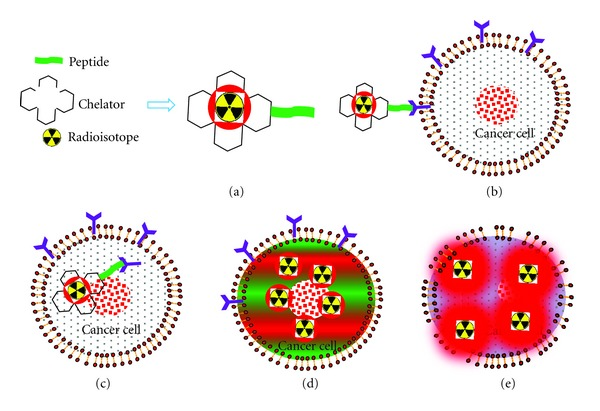
\includegraphics[width=12cm\textwidth]{Theory/therapy-peptide.jpg}
    \caption{A radionuclide is bound to a chelating agent, and with a peptide, the radiopharmaceutical targets the cancer cells. Figure is from citation [8] in the special curriculum. }
    \label{fig:therapy_chelator_peptide}
\end{figure}

%\section{Characteristics of therapeutic radionuclides}
\noindent    \textcolor{blue}{Whenever something is cited like (3), it means citation 3 in special curriculum}
Special curriculum p. 4: as mentioned above there are many requirements before a radiopharmaceutical can be used clinically, there are physical properties concerning the radionuclide, such as physical half-life, decay-mode and decay product, radiation energy and in-tissue range, and biological properties concerning the tracer such as tissue targeting, biological half-life, retention in tumor and the uptake in healthy tissue (3).  Thus, the radiopharmaceutical requires two components in which complement each other to deposit the dose in the cancerous tissue. 

In nuclear medicine, the effective half-life of the radiopharmaceutical is important as it takes both the physical half-life and the time it takes for the radiopharmaceutical to be cleared or excreted from the body (3). Thus it should be long enough to permit radiosynthesis and qauality control (handbook, chapter targeted radionuclide therapy). Should be compatible with the pharmacokinetics of localization in tumor and clearance from normal tissue. However, as for therapy, high radiation dose is desired, which is easier to achieve with shorter half life, so that should also be compensated for. The choice of radionuclide should match the uptake rate and the retention, to avoid radioactive waste handling and dose to healthy tissue (3). Therapautic radionucldies typically have half-lives  in order of a few hours to several days (9, p. 1) (special curriculum p. 4).\\

Knowledge about the decay products are also important, if unstable, how it the dose distributed, and how long range, half life etc, and if unstable, is the daughter contributing to a cytotoxic effect, or taking part of the natural processes in the body. \\

In addition, the chemical-biological properties are important, as it must be chemically possible to attach radionuclide to the targeting molecule. Also, the bond must be stable in the body, over a time period which is stable as long as the physical half life. (handbook p. 2185)\\ 

\noindent
Along with the ability to use radionuclides in therapy, radionuclides can also be used for diagnostic purposes with imaging, either with positron emitters (positron emission tomography) inwhich annihilates with atomic electrons close to the cite of decay, and sends out two 511 keV photons, or emission of a strongly fed gamma-decay energy which is detected (single photon emission tomography). The combination of a diagnostic and a therapautic agent with similar properties so that the biochemical uptake in the body is a new approach in which can give information of how the uptake is distributed in the body, and can image the state of decease after therapies (The beginning and development of the theranostic approach in nuclear medicine.... 86/90Y). This is called theranostics.. 

\section{Particle interaction in tissue}

Ionizing radiation are particles with sufficient energy to cause ionizations along the particle track, thus separating an atom and one or more electrons. The free electron(s) can ionize further, and the positive ion can cause undesired reactions. DNA is a large molecule with two strands bound in a double helix structure. Each strand is composed of sugar and phosphate groups, and nitrogenous bases which bind the two strands (biobook p. 11). These  bases are called adenine \& guanine amd cytosine \& thyamine (always bound pairwise), and are bound through weak hydrogen bonds which are exposed for strand breaks. The cell is equipped with an impressive repair mechanism, and unless both strands of the DNA is damaged, called a double stranded break (DSB), most damages are repaired. Radiation damages in the DNA can be caused directly by the ionizing particle or indirectly via free radicals, which are subject to other ionizations. Since the body contains large amounts of water, ionization of water molecules giving for instance H$^\bullet$ or OH$^\bullet$ are important damaging factors. Damages induced in the DNA can be lethal to the cell and either cause apoptosis or mutation in which can cause cancer. In therapy, the goal is to make malignant cells to undergo apoptosis, thus DNA is referred to as the target (book, p. 9). Choosing a particle with a high probability of inducing damage will induce multiple double stranded breaks if passing near by (special curriculum). 

Linear energy transfer (LET) describes the energy absorbed by the medium, and is defined as the average energy (typically in keV) deposited per unit length (typically measured in $\mu$m) of the density material (biobook, p. 101)

\begin{equation}
    \text{LET}=\frac{dE}{dx}
\end{equation}

To maximise the chances of inducing damages in the DNA and minimizing exposure of healthy tissue, choosing a particle with a high linear energy transfer is important in targeted radionuclide therapy. Figure \ref{fig:DNA_let} illustrates how $\beta^-$-particles, alpha-particles and auger electrons deposit energy on the scale of DNA. \\

Beta decays occur whenever there is an overweight in number of protons/neutrons. $\beta^-$: $n\rightarrow p+e^-+ \overline{\nu_e}$. The contrary $\beta^+$ decay: $p \rightarrow n+e^+ +\nu_e$. Neutron mass is higher than proton mass with $2m_e$ MeV/$c^2$, thus energy threshold for beta+ reaction must overcome this. If not high enough E, electron capture happens: $p+e^-_\text{atomic}\rightarrow n+ \nu_e$. For beta is distributed between three particles thus the energy is not discrete. Alpha decay occur when the nucleus is so large about to overcome Coulomb barrier. Thus emission of an alpha particle lowers the binding energy as the alpha particle carries a high B.E. These are discrete. Auger electrons are result from electron capture or internal conversion, which happens when a gamma-ray interacts electromagnetically with atomic electron, and emit with high energy. The vacancy in the atomic shell can lead to a cascade of X-rays and auger electrons with energies in the X-ray range. These energies are discrete, as the X-ray energy is discrete (minus atomic binding energy). From beta and sometimes alpha decay, the daughter nucleus is left in an excited state and decays by gamma-emission (all from special curriculum).  \\

\noindent A medium consists of positively charged nuclei and negatively charged electrons. Charged particles have a short range in a medium compared to neutral particles, as the Coulomb force forces the particle to interact continuously along the path either by scattering inelastic with the atomic electrons or scattering elastic with the nuclei. Elastic scattering is the less dominant process, where the energy loss is small, as long as the nuclei in the medium are larger than the incoming particle(Techniques for Nuclear and Particle Physics Experiments, William R. Leo, p.  21). \textcolor{red}{Inelastic collisions dominates where the atomic electrons are either excited or ionized (which citation???? Instrumentation book?)}. Under the assumption that the collision is elastic, the collision is head-on and the particle has high energy, the maximum energy transfer can be calculated using conservation of momentum and energy

\begin{equation} \label{eq:collision_E_transfer}
    Q_\text{max}=\frac{4m_eM}{m+M}E
\end{equation}

where $m_e$ is the mass of an atomic electron, M is the mass of the incoming charged particle and E is the kinetic energy of the incoming charged particle\footnote{https://ocw.mit.edu/courses/nuclear-engineering/22-55j-principles-of-radiation-interactions-fall-2004/lecture-notes/energydeposhcp.pdf}. While LET describes the energy transferred per unit length, the stopping power describes the energy loss of a charged particle per unit distance. The collision loss for heavy charged particles (protons and above) at high energies is therefor low. The stopping power for heavy charged particles (protons and up) is described by Bethe-Block.
\begin{comment}
\begin{equation}
    -\frac{dE}{dx} = 2\pi N_a r_e^2 m_e c^2\rho \frac{Z}{A}\frac{z^2}{\beta^2}\Big[\ln \Big( \frac{2m_e\gamma^2v^2W_\text{max}}{I^2} \Big)-2\beta^2 -\delta -2\frac{C}{Z} \Big]
\end{equation}
where
\begin{multicols}{2}
%$2\pi N_a re^2m_e c^2=0.1535 \text{ MeVcm$^2$/g} $\\ 
\noindent
$r_e: $ classical electron radius\\
$m_e: $ electron mass\\
$N_a: $ Avogadro's number \\
$I: $ mean excitation energy \\
$Z: $ atomic number of absorbing material\\
$A: $ atomic weight of absorbing material \\
$\rho: $ density of absorbing material \\
$z: $ charge of incident particle \\
$\delta: $ density correction \\
$C: $ shell correction\\ 
$W_\text{max}: $ maximum energy transfer in each collision\\
$\beta=v/c:$ incident velocity of the particle\\
$\gamma=\frac{1}{\sqrt{1-\beta^2}}: $ Lorentz factor

\end{multicols}

(Techniques in nuclear and particle physics p. 24).
\end{comment}
 As the particle slows down, the more energy per unit length will be deposited, as the charged particle picks up electrons. This is known as the Bragg peak. most of the energy is deposited near the end stop. The stopping power of heavy charged particles are proportional to the charge of particle and the inverse velocity squared. Therefor, particles with a higher charge will have a higher Bragg-peak and a shorter range in tissue, if energy was the same. This behaviour of heavy charged particles is especially useful in external beam therapy and is utilized to have a very specific dose over tumor as the dose before is low and the dose after bragg peak is zero (instrumentation, p. 27-28). \\

Electrons can experience energy loss either  from  collisions, or via the electromagnetic radiation that arises when electrons are loosing energy (bremsstrahlung), due to the small mass. However, for energies up to a few MeV, the collision energy loss dominates (Techniques for Nuclear and Particle Physics Experiments, WilliamR. Leo, p.  37). For electrons, the maximum energy transfer per collision is half of the initial energy, which means that electrons lose energy fast via collisions. Electrons scatters rapidly, and changes direction continuously due to the equal mass of the atomic electrons. The energy loss of electrons fluctuates much more than heavy charged particles which is due to much greater energy transfer per collision and to the emission of bremsstrahlung. To absorb major part of the electron's energy, is a few collisions, and results in greater range straggling.  (instrumentation p. 42)\\
 
Beta-electrons have a continuous spectrum of energies and absorption of beta decay electrons exhibit behavour which is well approximated to an exponential form (instrumentation p. 42). 
Low energetic electrons are small in mass to large angle deflection by scattering from nuclei (p. 48). 


\begin{comment}
\begin{equation}
    -\frac{dE}{dx}=2\pi N_a r_e m_e c^2\rho \frac{Z}{A}\frac{1}{\beta^2}\Big[ \ln \frac{\tau^2(\tau+2)}{2(I/m_ec^2)^2)} + F(\tau) - \delta - 2\frac{C}{Z} \Big]
\end{equation}

where $\tau$ is the kinetic energy of particle in $m_ec^2$ (instrumentation p. 37).  
\end{comment}

Photons and neutrons however are neutral particles and are not energy-degraded. Instead neutral particles are attenuated as a function of distance traversed x and the attenuation coefficient $\mu$ of the material 

\begin{equation}
    I = I_0 e^{-\mu x}
\end{equation}

where I is the intensity as a function of distance and $I_0$ is the intensity at x=0. 
 X-rays produced from a X-ray tube and gamma-rays degrades exponentially, thus have a high dose over a long distance. As gamma emitters are not directly used in targeted  radionuclide therapy, the gammaradiation following alpha or beta decay, or X-rays following electron capture or internal conversion needs to be taken into account.\\
 For high energetic X-rays, there is also a build up effect, where the photons induce ionizations, and the free electrons contribute to a higher dose. This is utilized in external beam therapy, maximizing the dose over the tumor. \\

Figure \ref{fig:particle_interaction} illustrates how various particles interact in a medium. For photons, there is an exponential tale, and for high energetic X-rays it is clear that there is a build up effect. For protons, the Bragg peak is very evident. For 22 MeV electrons, it is clear that there is 
bremsstrahlung energy loss due to the exponential tale. \\


\begin{figure}
    \centering
    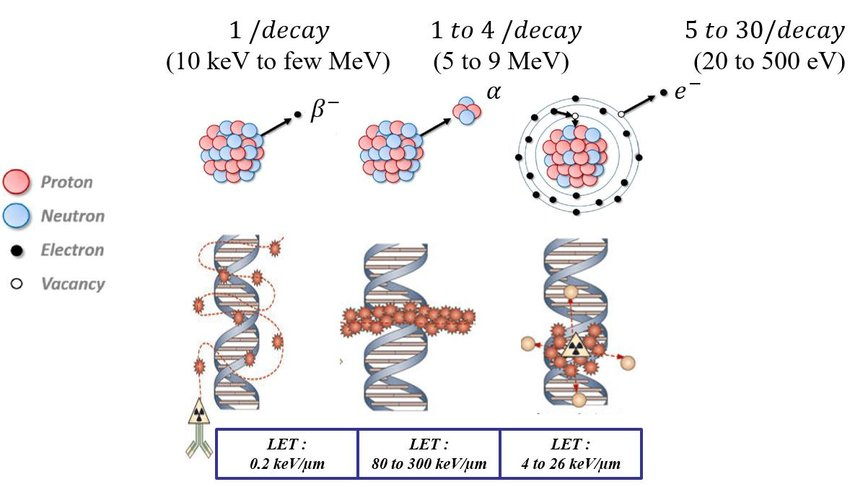
\includegraphics[width=10cm]{Theory/DNA_LET.jpg}
    \caption{The figure illustrates how $\beta^-$-particles, $\alpha$-particles and auger electrons deposit their energy on the scale of DNA. 
    
    \footnote{Accurately determining the number of Auger electrons per nuclear decay for medical isotopes - Scientific Figure on ResearchGate. Available from: https://www.researchgate.net/figure/Biophysical-properties-of-beta-alpha-and-Auger-electron-emitting-radionuclides-uper_fig1_334879307 [accessed 2 May, 2020]}}
    \label{fig:DNA_let}
\end{figure}


\begin{figure}
    \centering
    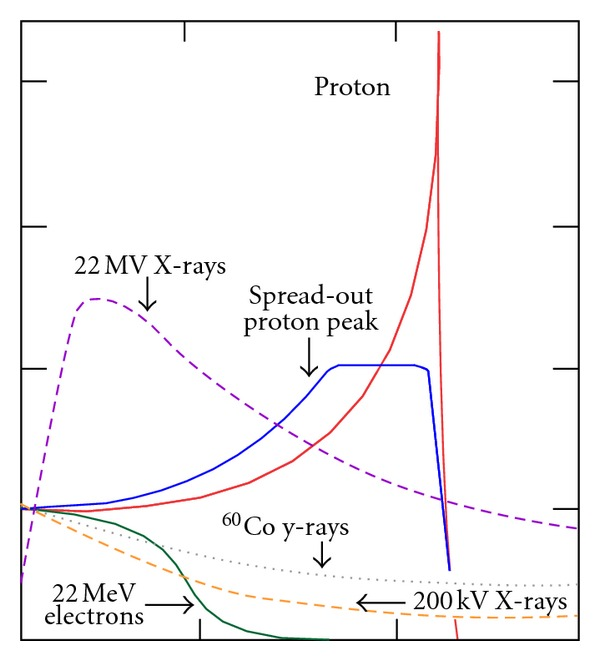
\includegraphics[width=0.6\textwidth]{Theory/Bragg-peak-and-Spread-Out-Bragg-Peak-SOBP-for-a-proton-beam-in-comparison-with-photon.jpg}
    \caption{Medium depth along x-axis, energy deposition in tissue (or dose?) on y-axis. Find citation in special curriculum. }
    \label{fig:particle_interaction}
\end{figure}



Figure \ref{fig:cell_dimension} shows an overview of the ranges of auger electrons, 5.3 MeV alpha particles, low and high energetic $\beta^-$ particles of 0.15 MeV and 1.7 MeV. Thus $\beta^-$-particles have a relatively long range in tissue, and can be up to a few mm dependent on the energy spectrum (handbook, chapter TRNT (TARGETED RADIONUCLIDE THERAPY). Beta-particles have relatively low LET and are thus suited for treating large tumors, but the dose to healthy tissue is hard to avoid.  Alpha-particles have short range in tissue, typically a one to a few cells in diameter. Has a high LET-value, radiation with LET=100 keV/$\mu$m has the distance between ionizing events is nearly identical to that between DNA strands increasing the probability of creating highly cytotoxic double strand breaks (handbook, TRNT). One of the major problems with alpha-emitters however is the decay products, as a typical alpha decay chain results in multiple emission of alpha and beta (??). For low energetic electron emitters such as auger emitters, the range is so low that in order to deposit energy in the DNA, must be incorporated into the cellular nucleus. Thus, it will only affect the cell targeted, and as we can see in figure \ref{fig:DNA_let} when incorporated into DNA, will induce many breaks and kill cell!!  (book: chapter targeted radionuclide therapy, whole paragraph) \\

\begin{figure}
    \centering
    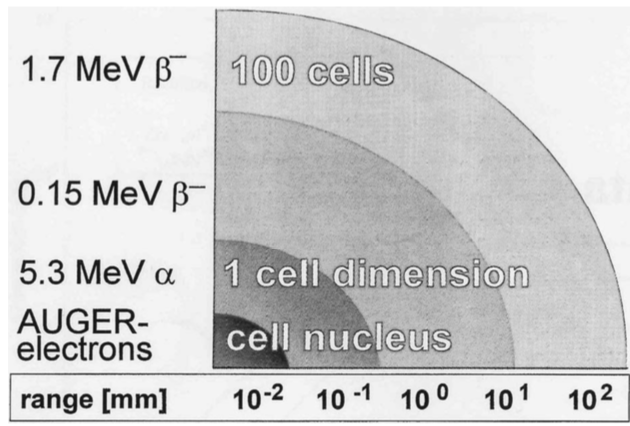
\includegraphics{Theory/cell_dimension.png}
    \caption{The figure illustrates the ranges of auger electrons, 5.3 MeV alpha particles and low and high energetic $\beta^-$ particles. }
    \label{fig:cell_dimension}
\end{figure}




\section{Production of radionuclides}
%The ideal radiopharmaceutical delivers a lethal dose to all cells within a tumor, while sparing normal tissue. ()

%(p. 2183): Also important to keep in mind that even with a uniformly distributed radionuclide, the dose received by individual cells can vary because of the differences in cross fires dose and the fraction of the radiation bound to the cell that is deposited in the tumor. This is particularly apparent for micrometastastic desease which presents as small clusters of tumor cells magnifying the impact of these factors. (p.2183): the success of radionuclide therapy is also critically dependent upon achieving homogeneous dose deposition within the tumor so that regrowth from an untreated subpopulation will be avoided. 
%(p.2185):Half life: should be long enough to permit radio synthesis and quality control and in some cases distribution to locations distant from the production site of the radiopharmaceutical. More importantly the half life shold be compatible with the pharmacokinetics of localization in tumor and clearance from normal tissue. Finally its generally easier to achieve higher radiation dose with shorter half-life radionucldies. 
%Cell culture expermiments have showsn that increasing the dose rate for low linear energy transfer radiation can lead to a greater degree of tumor control. 
The radionuclide availability is an important factor, and must obviously be high. Reactors, cyclotrons and natural decay chains have traditionally been used as radionuclide sources (Handbook of ... , p. 2185). Proton rich nuclei are typically produced in accelerators/cyclotrons using positively charged particles, and neutron rich nuclei are typically been products of fission or produced in the neutron flux resulting from fission in a reactor. Thus therapeutic radionuclides producing $\beta^-$-emitters needs neutrons, which are the main source of reactors. With research reactors today aging ([3], in special curriculum p. 10), alternative production routes to produce critical medical radionuclides. \\

There are many different production routes available for a single radionuclide, dependent on choice of target, particle beam and beam energy. The production route has an associated reaction cross section which is dependent on the beam energy. The nuclear cross section data is very important in optimization of production processes, achieving the maximum yield of the desired radionuclide combined with the minimum level of radionuclidic impurities ([9], in special curriculum p. 3). A high degree of radionuclidic purity is required for therapautic radiopharmaceuticals depending on the nature of the molecule that will be labelled, specific activity (GBq/mmol) may also be important consideration. It is impossible to chemically separate isotopes of the same element ([4], in special curriculum p. 10). We want to be sure that the what is injected into the patient does not have isotopic impurities which gives undesired dose to the tissue, nor will we have isotopes with no therapautic effect, both for most effective treatment, but especially in cases where the body does not excrete the element from the body, and we can have poisoning. Carrier-free production which are molecules which exclusively contain the desired radionuclides is desired because it gives the highest specific activity. The only option to minimize impurities is to choose an appropriate energy windown which minimizes the production of co-products. 

There already exists large amounts of information on neutron induced reactions. However the information on charged particle induced reactions is not as strong so we need more data on this behalf ([4] in special curriculum p. 10). Production of medical radionuclides should be cheap and available for everyday medical purposes. Cyclotrons good: Accelerators can be small in size and handled easily by medical personnel. Many hospitals which performs nuclear medicine even have a cyclotron facility on site, which is advantageous as its practical to avoid travelling logistics and to have medical radionuclide supply in proximity of examination/treatment site.  


%Selection of a radionuclide for targeted radionuclide radiotherapy must also take into account its chemical biological properties. 
%Chemical methods must be devised for attaching the radionucldie to the targeting molecule of interest without compromising the tumor localizing capacity of the molecule. In addition the bond between the radionuclide and the carrier molecule must be stable in the in vivo environment over a time period consistent with the physical half life of the radionuclide in order to minimize damage to normal organs. 


\begin{comment}

%\newpage
%Beta-emitting particles were the first ones which were used, long range (high energy) for large tumors and short range (low) energy  more than 2 mm range for long range particles

%Range of alpha-particles a few cell diameters, offering the prospect of matching the cell-specific nature of targeted molecular carriers with radiation having a similar range of action. Short range alpha particles also may be ideally suited for minimal residual disease settings applications in which radionuclide therapy has the greatest chance of making a meaningful clinical impact. These include treating micrometastasis, residual tumor margin left after surgival debulking, and tumors present in the circulation such as leukemia and lymphoma. Have much higher energies than beta paricles, and along with short range, have very high LET. Radiation at 100 keV  keV/$\mu$m has this quality because at this LET, the distance between ionizing events is nearly identical to that between DNA strands, increasing the probability of creating highly cytotoxic double DNA strand breaks. 

%Low energy electron emitters: deposit energy in subcellular dimensions. Can arise from two decay processes; internal conversion and electron capture. Both create inner atomic shell vacancies that are transferred by a series of rearrangments to outer atomic shells. the binding energy difference between the inner and outer subshells may then be transferred to other outer shell electrons, that are ejected from the atom. These electrons are called auger electrons, if they arise from higher shells and coster-kronig electrons if they originate from higher subshells. 

%\begin{figure}
%    \centering
%    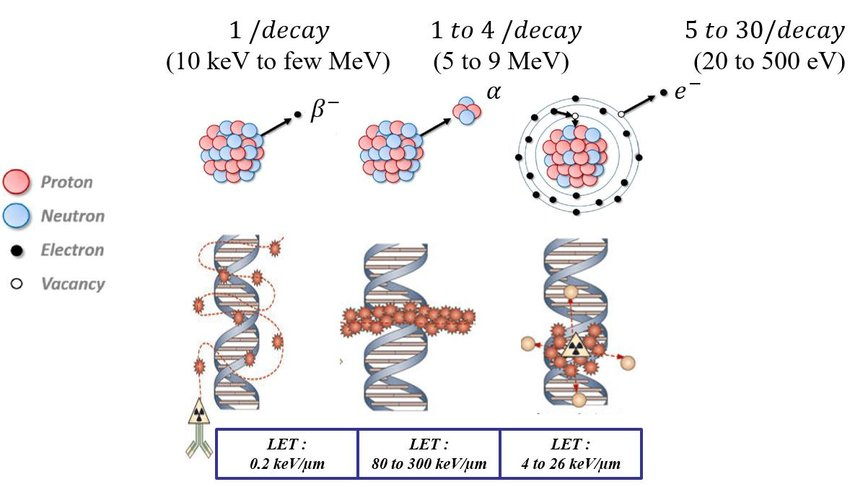
\includegraphics[width=10cm]{Theory/DNA_LET.jpg}
%    \caption{The figure illustrates how $\beta^-$-particles, $\alpha$-particles and auger electrons deposit their energy on the scale of DNA. 
    
%    \footnote{Accurately determining the number of Auger electrons per nuclear decay for medical isotopes - Scientific Figure on ResearchGate. Available from: https://www.researchgate.net/figure/Biophysical-properties-of-beta-alpha-and-Auger-electron-emitting-radionuclides-uper_fig1_334879307 [accessed 2 May, 2020]}}
%    \label{fig:DNA_let}
%\end{figure}

\begin{figure}
    \centering
    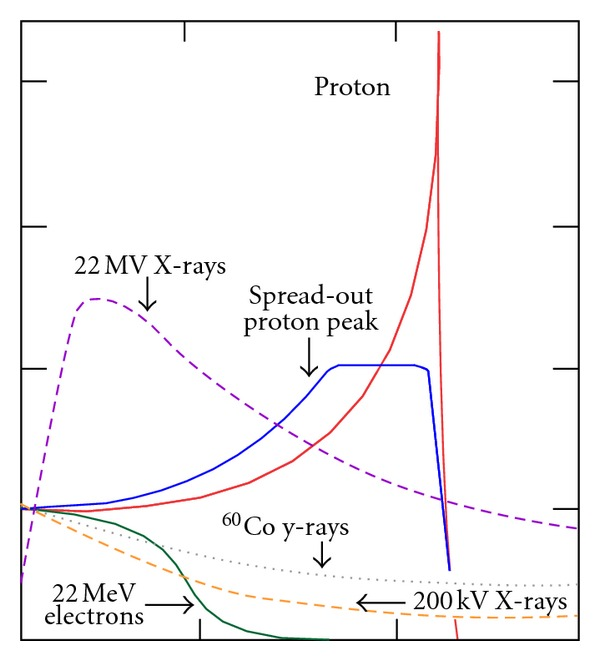
\includegraphics[width=0.6\textwidth]{Theory/Bragg-peak-and-Spread-Out-Bragg-Peak-SOBP-for-a-proton-beam-in-comparison-with-photon.jpg}
    \caption{Medium depth along x-axis, energy deposition in tissue (or dose?) on y-axis. Find citation in special curriculum. }
    \label{fig:particle_interaction}
\end{figure}


- What is targeted radionuclide therapy
- Biological effect
- Characteristics: half-life, decay mode, 
- LET, stoppingpower



\textcolor{blue}{Whenever something is cited like (3), it means citation 3 in special curriculum Special curriculum p.4:}  many requirements before a radiopharmaceutical can be used clinically, there are physical proper-ties concerning the radionuclide, such as physical half-life, decay-mode and decay product, radiationenergy and in-tissue range, and biological properties concerning the tracer such as tissue targeting,biological half-life, retention in tumor and the uptake in healthy tissue (3).  Thus, the radiopharma-ceutical requires two components in which complement each other to deposit the dose in the canceroustissue.  For the tracer, a rapid blood clearance and transport (6, p.  145) and high uptake and reten-tion in the tumor (9.  p.  2) (special curriculum p.  4) are important characteristics.  It can targetthe desired cells by for instance a specific receptor, enzyme, membrane, transporters or antigens (6,p.  145).  Radiometals are also used,  which consists of a bifunctional chelator,  which is a moleculecontaining molecules which can donate a lone pair of electrons, like nitrogen, oxygen or sulfur.  If theradiometal has an oxidation state of $3^+$, it will be tighlty bound by the chelator, and can transportedto the tumor (special curriculum p.  4-5). 

Dependent on size and geometry of the tumor, along with localization, a radionuclide decay mode and radiation range in tissue are important characteristics. For instance, if tumor is small and in a critical region must be ...., also if up to brain must be smaller than BBB. Characteristics of emission, half-life, production method, chemistry and biological behaviour (handbook of nuclear chemistry, p. 2181). 

The ideal radiopharmaceutical delivers a lethal dose to all cells within a tumor, while sparing normal tissue. 

(p. 2183): Also important to keep in mind that even with a uniformly distributed radionuclide, the dose received by individual cells can vary because of the differences in cross fires dose and the fraction of the radiation bound to the cell that is deposited in the tumor. This is particularly apparent for micrometastastic desease which presents as small clusters of tumor cells magnifying the impact of these factors. (p.2183): the success of radionuclide therapy is also critically dependent upon achieving homogeneous dose deposition within the tumor so that regrowth from an untreated subpopulation will be avoided. 
(p.2185):Half life: should be long enough to permit radio synthesis and quality control and in some cases distribution to locations distant from the production site of the radiopharmaceutical. More importantly the half life shold be compatible with the pharmacokinetics of localization in tumor and clearance from normal tissue. Finally its generally easier to achieve higher radiation dose with shorter half-life radionucldies. 
Cell culture expermiments have showsn that increasing the dose rate for low linear energy transfer radiation can lead to a greater degree of tumor control. 
Radionuclide availability: reactors, cyclotrons, natural decay chains have all been utilized as sources of radionuclides for targetred radionuclide therapy. A high degree of radionuclidic purity is required for therapautic radiopharmaceuticals depending on the nature of the molecule that will be labelled, specific activity (GBq/mmol) may also be important consideration 
Selection of a radionuclide for targeted radionuclide radiotherapy must also take into account its chemical biological properties. CHemical methods must be devised for attaching the radionucldie to the targeting molecule of interest without compromising the tumor localizing capacity of the molecule. In addition the bond between the radionuclide and the carrier molecule must be stable in the in vivo environment over a time period consistent with the physical half life of the radionuclide in order to minimize damage to normal organs. 
\end{comment}


%\subsection{Cyclotron production using deuterons}
%The deuteron is  losely bound particle, with a break up energy blablabla. 
%In order simulate the detueron beam, anderson and ziegler stopping power was used. blablabla just writted down from head. 

%Deuteron stopping power: 
%Anderson\&Ziegler stopping power formalism.
%Is just the addition of the two corrections density effect ad shell correction??






\section{$\mathbf{^{193m}}$Pt as a potential therapautic agent}
$^{193m}$Pt ($t_{1/2}$=4.33 days) is an auger-emitting isomer which decays by isomeric transition (100\%) to the long-lived $^{193g}$Pt groundstate ($t_{1/2}$=50 years) \cite{ShamsuzzohaBasunia2017a}. Radionuclides produced from deuterons on natural iridium such as $^{191}$Pt, $^{193m}$Pt, $^{192}$Ir and $^{194}$Ir are believed to have potential in medicine, like chemotherapy, brachytherapy, radioimmunotherapy and imaging (Tarkanyi et.al 2006). Platinum radionuclides are of special interest, as platinum is the main element in chemotherapautic agents such as cisplatin, which is a drug which is used clinically in treatment of testicular and ovarian cancer mainly, but also to treat esophagus, head and neck and bladder cancer\footnote{https://www.sciencedirect.com/science/article/pii/S0969804399000822?casa_token=ZLJ8YPQzGZMAAAAA:264QzKWpH8Kv6iHotiGMeoHTk8jKqmnoDgf709SrAD8BUWVwbRXriZbHgkYO_tHg-2qyX3Hvt9E}. Cisplatin  (cis-dichlorodiammine platinum(II)) is an inorganic molecule which contains one stable platinum atom surrounded by two clorine atoms and two ammonia molecules (NH$_3$). The cisplatin-molecule enters the cell nucleus, and binds to the DNA, example-wise shown in figure \ref{fig:cisplatin_DNA}, where the clorine-atoms are de-attached and the platinum-atom binds through covalent bonds to the DNA base guanine (and in some cases adenine, \textcolor{red}{is that correct?}), and breaks the bonds between the DNA nitrogeneous bases. Cisplatin thus targets the DNA. One of the major challenges with cisplatin is the chemical toxicity, but when auger-emitters such as $^{193m}$Pt or $^{195m}$Pt replace the stable platinum atom, the local auger-damage effect increases the chemical damage of cisplatin, suggesting that a smaller amount of the drug is required, and chemical toxicity can be avoided. \footnote{http://citeseerx.ist.psu.edu/viewdoc/download?doi=10.1.1.987.2577&rep=rep1&type=pdf#page=506, p. 493}.  \textcolor{red}{exactly how does it target the specific target cells, how is the uptake? how does the uptake of a healthy cell differ from cancer cells?}

By replacing either of the stable nitrogen atoms with the PET-radionuclide $^{13}$N ($t_{1/2}$=9.965 minutes), or by a radionuclide platinum, where $^{191}$Pt ($t_{1/2}$=2.83 days, decay by electron capture (100\%) to $^{191}$Ir (stable)) , $^{193m}$Pt and $^{195m}$Pt ($t_{1/2}$=4.010 days, decay by isomer transition (100\%) to $^{195g}$Pt (stable)) is of special interest, cisplatin can be used for imaging or therapy\footnote{https://www.sciencedirect.com/science/article/pii/S0969804399000822?casa_token=ZLJ8YPQzGZMAAAAA:264QzKWpH8Kv6iHotiGMeoHTk8jKqmnoDgf709SrAD8BUWVwbRXriZbHgkYO_tHg-2qyX3Hvt9E}, but therapy is most common. \\ 

\noindent 
As $^{191}$Pt is electron-capture emitter, can be used in imaging, with for instance 129.4 keV (38.0\%) or 172.19 keV (43.2\%). Combining $^{191}$Pt with a therapautic agent might be possible for theranostic pair with either $^{193m}$Pt or $^{195m}$Pt? Can be combined with therapy as it releases auger electrons? \\

%\subsection{Decay of $^{193m}$Pt}
Gamma-decay is a result of de-exitation of a nucleus with the release of a photon equal to the energy difference between the two states. The typical half-life of a populated excited state is less than $10^{-9}$ seconds, and states with longer half-lives are called isomeric states (Krane p. 175). This isomer decays by isomeric transition. In all decays, there are certain quantities which needs to be conserved; angular momentum, partiy. Krane says that a multipole of order $\ell$ transfers angular momentum $\ell \hbar$ per photon (Krane p.333). A nuclear state has a definite angular momentum $\ell$ (ang mom + spin?) and parity, and if a gamma transition is to happen between two states the photon must connect the two states by conserving angular momentum and parity. In order for the quantity $\ell$ to be conserved, the angular momentum can be integers between 
\begin{equation}
    |I_i - I_f \leq \ell \neq I_i + I_f
\end{equation}
where i is initial and f is final. I is the total spin (angular momentum and spin). The parity decides wether  the radiation is electric multipole or magnetic multipole (equations from Krane p.311)

\begin{equation}
\pi (ML)= (-1)^{\ell+1}, \quad \pi(EL) = (-1)^\ell    
\end{equation}

There are three populated states, the isomer state at 149.8 keV, with nuclear spin $13/2^+$ (4.33 d), a state at 14.3 keV with nuclear spin $5/2^-$ (2.52 ns), a state at 1.6 keV with nuclear spin $3/2^-$ (9.7 ns) and the ground state at 0.0 keV with nuclear spin $1/2^-$ (50 y)\footenote{https://www.nndc.bnl.gov/nudat2/getdecayscheme.jsp?nucleus=193PT&dsid=193pt\%20it\%20decay\%20(4.33\%20d)&unc=nds
}\cite{ShamsuzzohaBasunia2017a}. 

For the decay of $^{193m}$Pt (E level=149.8 keV) to the excited state (E level=14.3 keV), the spin and parity changes from $13/2^+$ to $5/2^-$, which gives possible values for $\ell=4,5,6,7,8,9$. The electric decays have even parity when $\ell$=even, and magnetic has even when $\ell=$odd. If parity is unchanges in the decay ($\Delta\pi$=no), the electric multipoles are even and magnetic multipoles are odd. If the parity does change ($\Delta \pi$=yes) there would be odd electric and even magnetic multipoles. Hence for the possible transitions between $13/2^+$ to $5/2^-$ are whenever $\Delta \pi$=yes and $\ell=4,5,6,7,8,9$, which gives possible M4, E5, M6, E7, M8 and E9 transitions. \\

In general, the lowest possible multipole dominates, and the emission of a multipole of one order higher  ($\ell+1$ than $\ell$) is reduced by a factor ca. $10^{-5}$ (Krane, p. 335). Thus a multipole of order 4 or 5 has a low probability of occuring and thus the isomer has a long half-life. In comparison, the decay from $5/2^-$ to $3/2^-$ givespossible radiation $\ell=1,2,3,4$, $\Delta\pi$=no, gives possible M1, E2, M3, E4 and the same for decay from $3/2^-$ to $1/2^-$- 

Whenever gamma-decay is possible, another process called internal conversion is competing. It is an electromagnetic process where the nucleus electromagnetically with the atomic electrons, and an atomic electron is emitted instead of the photon (Krane, chapter 10, p. 341). The kinetic energy of the emitted electron is the transition energy minus the electron binding energy 

\begin{equation}
    T_e = \Delta E -B
\end{equation}

where B is the binding energy. The emitted electron is called a conversion electron, and the energy is comparable to the gamma-ray energy. The conversion electron varies with the atomic orbital (Krane, p.??), and the electrons following internal conversion are in a spectrum of different discrete energies. The transition energy must be higher than the electron binding energy, and as a consequence the electron is labelled with the shell it was emitted from (remember that atomic shells are labelled with n: n=1=K, n=2=L, n=3=M, n=4=N, etc). \\

\noindent 
For $^{193m}$Pt, internal conversion is highly favoured before gamma-decay, thus the observed gamma in gamma-ray spectroscopy is difficult. The total probability ois the summed decay probability for gamma-decay and internal conversion 

\begin{equation}
    \lambda = \lambda_\gamma + \lambda_\text{IC}
\end{equation}

and the internal conversion coefficient $\alpha$ can be defined as 
\begin{equation}
    \alpha = \frac{\lambda_\text{IC}}{\lambda_\gamma}
\end{equation}

High values for $\alpha$ indicates high probability of internal conversion relative to the probability of gamma emission but the coefficient diverges towards infinity when $\lambda_\gamma$ reaches towards zero, which for instance is when he gamma transition is zero. In general, the coefficient increases $Z^3$, which will give a much greater coefficient for heavy nuclei than for lighter nuclei. In addition the coefficient decreases rapidly (ca. E$^{-2.5}$) with increasing transition energy. The multipole order also affects the coefficient, where a higher multipole order indicates a higher value. For higher atomic shells than the K shell (n=1) the coefficient decreases like $n^{-3}$ (Krane chapter 10, p. 346). \\

\noindent 
From a therapautic point of view, the most important process is the process which occurs after the release of the conversion electron. There is a vacancy is the shell following the emission of the atomic electron, and an electron from a higher shell or subshell fills  this vacancy. Radiative or nan-radiative processes can take place after to conserve energy \footnote{https://sci-hub.tw/https://doi.org/10.1118/1.596927}. To conserve energy, an X-ray with the energy equal to the difference between the atomic states can be emitted, or that X-ray can interact electromagnetically with atomic electrons in same subshell, a higher subshell or shell (remember shell: n=1,2.., subshell: spdf..). Dependent on where the ejected electron originated from, the electrons are called super Coster-Kronig, Coster-Kronig or auger electrons respectively. In practice the vacancy moves up to higher atomic shells and the result is a cascade of electrons and Auger electrons, until the reaction "fades out". Due to the low energies, they need to be located close to the cellular nucleus or incorporated into the DNA for induce damage (Handbook of nuclear chemistry, p. 2203). When incorporated into DNA has they are equally almost effective as alphaemitters \cite{Howell1991} + handbook p. 2203). 
\newpage


\begin{comment}
\textcolor{red}{here write about gamma-decay and that the probability for M6 or whatever transition is improbable}. The populated isomer states decays from 149.8 keV to 14.3 keV releasing a 135.50 keV photon (0.1145475\%), from 14.3 keV to 1.6 keV releasing a 12.634 keV photon (0.70\%), and from 1.6 keV to the ground state releasing a 1.642 keV photon (0.0321). The photon abundance is thus low, and this isomer is not well suited for imaging. Due to the low intensity of the gamma-rays, it might be difficult to detect. There are X-rays too, but they overlap with other nuclei. Since the gamma-rays are weak, the IC probabilities are 99.89\%, 99.33\% and 99.99\% for each state respectively, calculated by subtracting 100 - gamma-intensity \footnote{http://citeseerx.ist.psu.edu/viewdoc/download?doi=10.1.1.987.2577&rep=rep1&type=pdf#page=506, p. 496}. This also indicates that the phondon abundance is very low, as well  high very high probality of low energy auger electrons.

In all decays, there are certain quantities in which needs to be conserved; angular momentum ($\ell$) and parity (maybe $\ell$ should be written as L instead??). Krane says that a multipole of order $\ell$ transfers angular momentum $\ell\hbar$ per photon (Krane, p. 333). A nuclear state has a definite angular momentum (angular momentum and spin) and parity, and if a gamma-transition is to happen between two states, the photon must connect the two states by conserving angular momentum and parity. In order for the quantity $\ell$ to be conserved, the angular momentum can be integer values between
\begin{equation}
|I_i-I_f| \leq \ell \leq I_i + I_f
\end{equation}
For the decay of $^{193m}$Pt (E level=149.8 keV) to the excited state (E level=14.3 keV), the spin and parity change is from $13/2^+$ to $5/2^-$, so $\ell=4,5,6,7,8,9$. The parity decides the wether the radiation is electric multipole or magnetic multipole (equations from Krane p. 331), 

\begin{equation}
    \pi(ML) = (-1)^{\ell+1}, \quad \pi(EL)=(-1)^{\ell}
\end{equation}
 
The electric decays have even parity when $\ell$=even, and magnetic has even when $\ell$ is odd. If parity is unchanged in the reaction ($\Delta \pi=$no), the electric multipoles are even and magnetic multipoles are odd. If the parity does change ($\Delta\pi=$yes), there would be odd electric and even magnetic multipoles. Hence the possible transition from $13/2^+$ to $5/2^-$ are whenever $\Delta \pi=$yes and $\ell=4,5,6,7,8,9$, which gives possible M4, E5, M6, E7, M8 or E9. 

In general, the lowest possible multipole dominates, and the emisssion of multipole of one order higher (L+1 than L), is reduced by a factor ca $10^{-5}$ (Krane p. 335, important!!). Thus, a multipole of order 4 or 5 has a low probability of occuring and thus the isomer has a long half life.  
In comparison to decay from isomer state, decay from $5/2^-$ to $3/2^-$ gives possible radiation, $\ell=1,2,3,4$, with no parity change, and $\Delta \pi=$no, gives possible M1, E2, M3, E4, and from $3/2^-$ to $1/2^-$ gives $\ell=1,2,3,4$, which also gives M1,E2, M3, E4. 

Half life: the decay rate constant is the sum of the decay rates of all the populates states  transitions, $\lambda=\lambda_{13/2^+} + \lambda_{5/2^-}+ ...$. 







\subsection{Gamma-decay and isomeric transition}
Gamma-decay is the lowering of the excitation energy by the release of a photon, with an energy $\Delta$E equal to the energydifference in the two states. The typical half lives of gamma-emission are less than $10^{-9}$ seconds, however, longer lived states of a nucleus which is not the ground state is called an isomer, and the gamma-decay of an isomer state is called isomeric transition (Krane, p. 175). Whenever gamma-decay is possible, another process called internal conversion is competing. It is an electromagnetic process, where the nucleus interacts electromagnetically with the atomic electrons, and an electron is emitted instead of the photon (Krane, chapter 10, p. 341). The kinetic energy of the emitted electron is the transition energy minus the electron binding energy

\begin{equation}
    T_e = \Delta E - B
\end{equation}

where B is a positive number (even though bound states are negative??). The electron is called a conversion electron, and this electron is high in energy and mathces the gamma-energy. 
The electron binding energy varies with the atomic orbital (Krane), and the electrons emitted following internal conversion are in a spectrum of different discrete energies. The transition energy must be higher than the electron binding energy, and as a consequence, the electron is labelled with the shell that it was emitted from. (remember, n=1=K, n=2=L, n=3=M, n=4=N) \\ 

In the case of the decay of $^{193m}$Pt, internal conversion is highly favoured instead of gamma-decay (the intensity of the gammas are very weak). The total decay probability is the summed decay probability for gamma-decay and internal conversion
\begin{equation}
\lambda = \lambda_\gamma + \lambda_{IC}    
\end{equation}

and the internal conversion coefficient $\alpha$ can be defined as
\begin{equation}
    \alpha = \frac{\lambda_{IC}}{\lambda_\gamma}
\end{equation}

High values of $\alpha$ indicates high probability of internal conversion, relative to probability of gamma-emisson, but the coefficient diverges towards infinity when $\lambda_\gamma$ reaches towards zero, which for instance is when the gamma-transition is zero. In general, the coefficient increases as $Z^3$, which will give a much greater coefficient for heavy nuclei than for lighter nuclei. In addition the coefficient decreases rapidly (ca. $E^{-2.5}$) with increasing transition energy. The multipole order also affects the coefficient, where a higher multipole order indicates a higher value. For higher atomic shells than the K shell (n=1), the coefficient decreases like $n^{-3}$ (Krane, chapter 10, p. 346). \\

\noindent 
In therapy, the most important process is the process which occurs after the release of the conversion electron. There is a vacancy in the shell where the conversion electron was emitted, and an electron from a higher shell drops down to this energylevel, with the release of an X-ray with an energy equal to the difference between the energy state of the two shells, $\Delta E$.\textcolor{red}{ If the transition is an electron from an L shell drops to K shell, and an electron from the L shell is ejected, the processes is called a KLL transition, and the energy of the auger electron is $E_{auger}=E_K - E_{LL}$ (Prasad A. Naik, in Encyclopedia of Spectroscopy and Spectrometry, 1999)\foonote{https://www.sciencedirect.com/topics/chemistry/auger-process}. If the vacancy is filled with an electron from the same shell (or subshell) but the ejected electron is from another shell, the electron is called a coster-kronig electron (like LLM, electron vacancy is moving from L to L and electron in M is emitted), and if the whole process occurs in the same shell, it is called a super coster-kronig process (MMM) }

The energy of the X-rays are lower in energy than the gamma-rays, typically. If one of the X-ray photon interacts within the atomic electrons (via photoelectric effect), the electron (which is called an auger electron) will be emitted with the energy of the X-ray minus the atomic binding energy  (Handbook of NUclear chemestry, p. 390)
\begin{equation} \label{eq:energy_auger}
    T_{a.e.}=\Delta E_{x-ray}-B
\end{equation}

From the vacancy from the auger electron, a new electron can take this place and release another X-ray. The auger electron can cause further ionizations in the atom, either by interaction it self, or from X-rays following the de-exication of another atomic electron by the vacancy. Thus it is possible to have a cascade of electrons and X-rays. The secondary electrons caused by the auger electron can lead to a cascade of new short-range electrons and X-rays, which are typically have ranges of nm in tissue (Handbook of nuclear chemistry p. 2203). Since the X-ray energy is in the low energy region, the auger electrons have low energies (from equation \ref{eq:energy_auger}).  

Since auger emitters are short range, they are very precise, and do only harm when bound to DNA or when incorporated into the cellular nucleus (handbook of nuclear chemistry, o. 2204), which means that no neightbooring cells will be affected. 

\textcolor{red}{After IC-process, vacancy is produced in an inner atomic shell (n) or subshell (like l=spdf). Vacancies in inner atomix orbitals are unstable, filled by electrons from higher energy levels. 4 processes, radiative X-ray transition, non-radiative transitions of auger, Coster-Kronig and super Coster-Kronig. move primary vacancies to higher shells or subshells. The non-radiative transitions involves multiplication of vacancies in the higher shells and subshels since two new vacancies are produced for each filled vacancy. Whenever energetically possible, super CS transitions dominate the other types. Thus the inner shell vacancies move upward to the valence and near valence shells of the atom, copious emission of electrons occur. Since the transition energies are very small for the higher shell transitions, the electrons ejected possess very small energies and is extremely short range (few nm) in biological matter, find a citation here, numb 8 in chapter. }
\end{comment}

\textcolor{red}{Energy loss of low E auger electrons. In this energy region, is due to collision loss, not bremsstrahlung. Deflects frequently due to low mass, and the max energy loss is $T_e/2$ per collision, as described in equation \ref{eq:collision_E_transfer}. }

\newline
General stuff $^{193m}$Pt: Cellular nucleus is approximately 6$\mu$m, while thickness of DNA is ca 2 nm (wikipedia). Range of the electrons from the decay is between 3.29nm-231$\mu$m, according to simulation done by Howell (1992) \cite{Howell1992}, so well within cellular nucleus. In its decay, it emits 26.4 coster-konig and auger electrons (energy realeased per decay: 10.353 keV) and internal 3 conversion electrons (energy released per decay: 126.738 keV). According to the simulation, an additive 12.345 keV is for X-ray energy deposition per decay. 

Production: there are multiple ways that this isomer can be produced, either in a neutron field in a reactor, or in a charged particle accelerator like a cyclotron: $^{192}$Pt(n,$\gamma$) or via $^{192}$Os($\alpha$,3n). One of the issues with production is that 193mPt (and 195mPt) are difficult to produce with high specific activity \cite{Qaim2017c}, and are not well investigated. This study gives an examination of a new route. Many reasons, reactors are on their way out, and Osmium is a poisoneous and difficult target to work with, so using iridium as target is easy, (expensive though?) and the production of radionuclides below iridium is evidently in this work and in papers tarkanyi et al (2006,2019) low. 

By itself, not useful for imaging. 191Pt and 195mPt can. Can replace stable N with 13N, but the half life is so short that the radionuclide can not image the distribution it self, so not as a theranostics pair?? or does cisplatin distribute so fast within the body? 



\begin{figure}
    \centering
    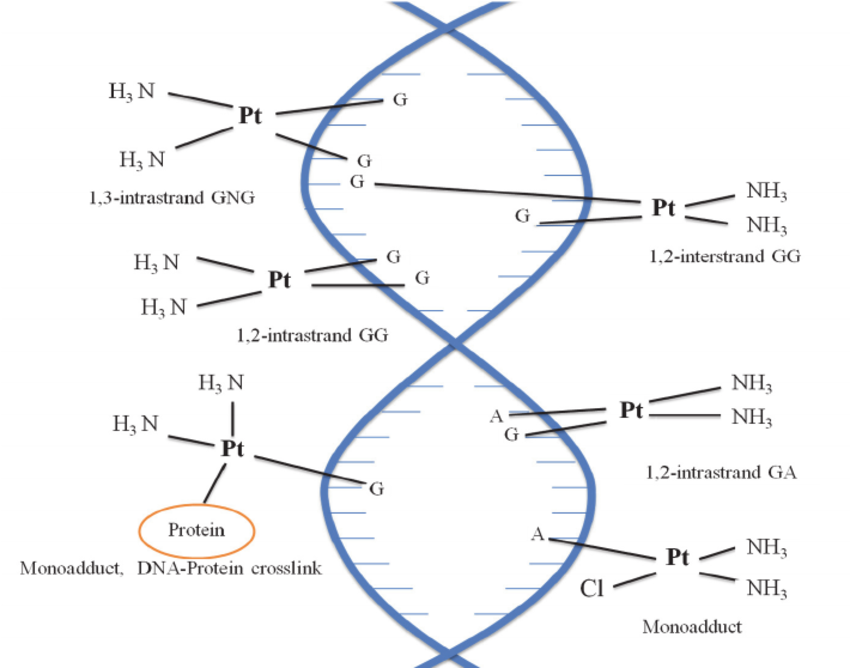
\includegraphics[width=0.5\textwidth]{Theory/cisplatin_DNA.png}
    \caption{A DNA Repair Protein BRCA1 as a Potentially Molecular Target for the Anticancer Platinum Drug Cisplatin - Scientific Figure on ResearchGate. Available from: https://www.researchgate.net/figure/Common-cisplatin-DNA-adducts-and-functions-For-instance-the-platination-of-human-serum_fig2_221919257 [accessed 12 Apr, 2020]. }
    \label{fig:cisplatin_DNA}
\end{figure}
Pt-poisoning 




%\section{General nuclear reaction theory}
\chapter{General nuclear reaction theory}

\textcolor{red}{paragraph based on special curriculum}
\textcolor{red}{need to rewrite this part as some of this is already mentioned above.. }
Medical radionuclides can be produced directly using charge particle (cyclotron) or neutron beams (reactors), or indirectly using radionuclide generators or fission (reactor). Medical radionuclides are typically produced in reactors, cyclotrons or by a longer lived-parent decaying into a short-lived daughter in a radionuclide generator system. In general, the production should be cheap, available. Today many radionuclides are only produced in reactors, which is the main source of neutrons, and with reactors aging (Chai Hong Yeong, Mu hua Cheng, and Kwan Hoong Ng. Therapeutic radionuclides in nuclear medicine: Current and future prospects. Journal of Zhejiang University: Science B,
15(10):845–863, 2014.), we need alternative routes to produce critical radionuclides. Cyclotrons have many benefits, like size so that it can be produced directly at the site of usage. One of the major disadvantages is that there is a need to enriched targets to get the desired reaction, and those can be very expensive. Along with high beam intensity the melting of the target can give challenges, so target cooling technqueis need to be there.    

In order to create isotopes, nuclear reactions need to occur. There are many different production routes available for a single radionuclide, which is dependent on multiple factors such as choice of target, incident particle-beam and beam energy. To each reaction route, there is an corresponding excitation function which tells us how probable the reaction channel is at various energies. The nuclear reaction data is very important for the optimization of the product, achieving minimal level of isotopic impurities and maximum yield (S M Qaim, R Capote, and F Tarkanyi. Nuclear Data for the Production of Therapeutic Radionuclides.
Trs 473, (473):395, 2011., p. 3). \\

Isotopic purity is important as it is impossible to separate isotopes of the same element \cite{Qaim2017c}. An undesired radionuclided can lead to undesired dose to healthy tissue, and a non-radioactive nuclide may lead to  poisoning (if large amounts injected), but it will not have any therapautic effect. This is especially important when working with poisoneos elements such as platinum. The only option to minimize isotopic impurities is to choose an appropritate energy window. 


Using charged particles instead of neutrons allows for measurement at multiple energies as the particle energy degrades in the foils. The neutron energy is not degraded in the same way, due to electric neutrality, thus can only give cross section at one single energy. 


\section{Radioactive decay law}
\textcolor{red}{where to place this? }

From here based on Krane chapter 6 \footnote{https://faculty.kfupm.edu.sa/phys/aanaqvi/Krane-Ch-6.pdf}

The activity of a nucleus is defined as the number of decayed nuclei per unit time of a radioactive product, which is equal to the radioactive decay rate 

\begin{equation} \label{eq:activity_decayrate}
   A =  \frac{dN}{dt}=-\lambda N
\end{equation}

where N is the number of nuclei, t is the time and $\lambda$ is the decay constant. Solving equation \ref{eq:activity_decayrate} gives number of decayed products at time t
\begin{equation} \label{eq:N(t)}
    N(t) = N_0 e^{-\lambda t}
\end{equation}

\noindent 
Since $N\propto$A, the relations $\frac{N_0}{A_0}=\frac{N(t)}{A(t)}$ are valid, and we can rewrite the equation \ref{eq:N(t)} to

\begin{equation} \label{eq:activity_decaylaw}
    A(t) = A_0 e^{-\lambda t}
\end{equation}


This accounts for single nucleus decaying into a daughter product, without anything first decaying into the parent nucleus. However it is common that a radioactive nucleus decays into another radioactive nucleus. Hence the daughter activity will increase due to feeding from the parent.
%The number of decayed nuclei N of nucleus i with a n-decay chain is then
%\begin{equation}
%    dN_i = \lambda_{i-n}N_{i-n}dt - ... -\lambda_{i-1}N_{i-1}dt - \lambda_iN_idt
%\end{equation}
For multiple decay, Bateman equation is used describing the activity in nucleus n of the decay chain \textcolor{red}{(Voyles2018, which article??)}

\begin{equation} \label{eq:ndecay_chains}
    A_n = \lambda_n \sum_{i=1}^n \Big[ \Big( A_{i,0}\prod^{n-1}_{j=i}\lambda_j \Big)\cdot \Big( \sum_{j=i}^n \frac{e^{-\lambda_j t}}{\prod_{i\neq j}^n (\lambda_i - \lambda_j)} \Big) \Big]
\end{equation}

where $A_n$ is the activity of nuclei n in the decay chain, with the corresponding decay constant $\lambda_n$. The equation sums over all nuclei in the decay chain. $A_{i,0}$ is the initial activity of nucleus i, and j is the nucleus which is feeding into nucleus i. 

\noindent 
If a target of stable nuclei is assumed, which is exposed to a particle beam which induces various nuclear reactions, the constant rate of production of a specific reaction is dependent on the number of target nuclei, the current of flux of the particle beam and the reaction cross section

\begin{equation}
    R = N_T \Phi \sigma
\end{equation}

\noindent 
where R is the production rate, $N_T$ is the number of target nuclei, $\Phi$ is the beam current or flux and $\sigma$ is the reaction cross section. In the assumption of the production rate being a constant value, the number of transformed target nuclei is small in comparison to the total number during the irradiation time. The number of produced nuclei from a specific reaction per unit time is thus thus the produced nuclei minus the decayed nuclei (activity)
\begin{equation}
    dN = Rdt - \lambda N dt
\end{equation}

which has the solution

\begin{equation}
    N(t) = \frac{R}{\lambda}(1-e^{-\lambda t})
\end{equation}

From equation \ref{eq:activity_decayrate}, the total activity produced during irradiation time t is thus 

\begin{equation} 
    A(t) = R(1-e^{-\lambda t}) = N_T \Phi \sigma (1-e^{-\lambda t})
\end{equation}

At the end of beam, the activity is denoted as $A_0$, and t is the irradiation time:
\begin{equation} \label{eq:activity_eob}
    A_0 = N_T \Phi \sigma (1-e^{-\lambda \Delta t_\text{irr}})
\end{equation}

\noindent 
When a target is irradiated, the activity of the product nucleus will increase until secular equilibrium is achieved, which is when the product rate and decay rate are constant. Hence it is not necessary to irradiate a target for more than 2-3 half lives.\\

\noindent 
If a spectrum is counted at a delay time $\Delta t_d$ after end of beam with a counting time $\Delta t_c$  the total number of decayed products are 

\begin{equation}
    N_D = \int_{\Delta t_d}^{\Delta t_d + \Delta t_c} A(t) dt
\end{equation}

Using equation \ref{eq:activity_decaylaw} for A(t), the solution to the above equation is 
\begin{equation} \label{eq:numb_of_decayed}
    N_D= \frac{A_0}{\lambda}e^{-\lambda \Delta t_d}(1-e^{-\lambda \Delta t_c})
\end{equation}

which again is equal to
\begin{equation}
    N_D = \frac{A(t)}{\lambda} (1-e^{-\lambda \Delta t_c})
\end{equation}

We can only know the number of decayed products which are detected. This is dependent on the efficiency of the detector, the intensity of the gamma-rays and the true number of decayed products

\begin{equation}\label{eq:Ngamma}
    N_C  = N_D \epsilon I_\gamma
\end{equation}

where $N_C$ is the number of observed/counted gamma-rays, $\epsilon$ is the efficiency of the detector and $I_\gamma$ is the gamma-ray intensity.\\ 

\noindent
Thus, we can obtain an expression for $A(t)$ after a delay time: 

\begin{equation} \label{eq:Final_Expression_A}
    A(t) = \frac{N_C \lambda}{\epsilon I_\gamma (1-e^{-\lambda \Delta t_c})}
\end{equation}

\noindent 
Again using \ref{eq:activity_decaylaw} for A(t), the above expression can be rewritten using $A_0$ and the delay time $\Delta t_d$

\begin{equation} \label{eq:Final_Expression_A0}
    A_0 = \frac{N_C \lambda }{\epsilon I_\gamma (1-e^{-\lambda \Delta t_c})e^{-\lambda \Delta t_d}}
\end{equation}
\begin{comment}
Combining equation \ref{eq:activity_eob} and \ref{eq:numb_of_decayed}, total number of decayed products is

\begin{equation} \label{eq:finalN_D}
    N_D= \frac{N_T \Phi \sigma}{\lambda}(1-e^{-\lambda \Delta t_\text{irr}})\cdot e^{-\lambda \Delta t_d}\cdot (1-e^{-\lambda \Delta t_c})
\end{equation}

Combining equation \ref{eq:Ngamma} and \ref{eq:finalN_D}, we get the following expression 

\begin{equation}
    \frac{\epsilon I_\gamma}{N_C}=\frac{N_T \Phi \sigma}{\lambda}(1-e^{-\lambda \Delta t_\text{irr}})\cdot e^{-\lambda \Delta t_d}\cdot (1-e^{-\lambda \Delta t_c})
\end{equation}

From here, $A_0$ is the following equation \ref{eq:activity_eob}

\begin{equation}
    A_0 = \frac{\epsilon I_\gamma \lambda}{N_C}\cdot e^{-\lambda \Delta t_d}\cdot  (1-e^{-\lambda \Delta t_c})
\end{equation}





%\begin{equation}
%    \sigma = \frac{A_0 }{N_T \Phi (1-e^{-\lamda \Delta t_\text{irr}})}
%\end{equation}

\begin{equation}
 \Phi = \frac{A_0 }{N_T \sigma (1-e^{-\lamda \Delta t_\text{irr}})}    
\end{equation}


\end{comment}

%In a detector, we can only know the number of decayed products from which are registered. Whether the detector detects or not is dependent on efficiency of detector, the intensity of the gamma-rays and the true number of decayed products

%\begin{equation}\label{eq:Ngamma}
%    N_\gamma  = N_D \epsilon I_\gamma
%\end{equation}

%where $N_\gamma$ is the number of observed gamma-rays, $\epsilon$ is the efficiency of the detector and $I_\gamma$ is the gamma-ray intensity. Combining equation \ref{eq:finalN_D} and \ref{eq:Ngamma}, the get the following expression 

%\begin{equation}
%    \frac{\epsilon I_\gamma}{N_\gamma}=\frac{N_T \Phi \sigma}{\lambda}(1-e^{-\lambda \Delta t_\text{irr}})\cdot e^{-\lambda \Delta t_d}\cdot (1-e^{-\lambda \Delta t_c})
%\end{equation}


\section{Nuclear reactions and reaction cross sections}

A nuclear reaction occurs when a collision between two nuclei or a nucleus and a subatomic particle takes place. Collision between an accelerated subatomic particle or small nucleus and target nuclei is common in isotope production. A nuclear reaction is denoted as
\begin{equation}
    X(a,b)Y
\end{equation}

\noindent where X is the target, a is the incoming projectile, b is the outgoing decay channel and Y is the product of the nuclear reaction (Krane, chapter 11.1). There are multiple processes which can occur, radiative capture is the process where a particle is captured and a $\gamma$-ray is emitted in a (x,$\gamma$) process. If the incoming and outgoing particle is the same, it is a scattering process, where elastic scattering leaves the target nucleus in the energy same state, and inelastic if the target nucleus is in an excited state. In these type of experiments however, we are interested in emission of particles to create products in which we can measure the reaction cross section. \\

In a nuclear reaction, the total energy and linear momentum, proton and neutron number, angular momentum and parity are conserved quantities (assuming no meson formation) (Krane, p.380). In the low energy-region in which isotope production typically takes place (\textcolor{red}{<80 MeV}?), compound nucleus reactions take place, where an incoming particle and target nucleus merges by sharing the kinetic energy on all nucleons, and particle emission takes place to reduce the excess energy. \textcolor{blue}{\footnote{blue text:https://web-docs.gsi.de/~wolle/TELEKOLLEG/KERN/LECTURE/Fraser/L24.pdf }Involves nucleon nucleon interactions, lead to a complete thermal equlibrium inside the CN. Releases energy by emission of neutrons, protons, alpha particles and gamma rays. A consequence of equilibrium is that the decay of CN should not depend on the way it was formed. "forgets" in all the collisions. Consequently, the decay of the compound nucleus depends only on the mass and atomic numbers, excitation energy and angular momentum.} The contrary are direct reactions, where an incoming particle interacts (over such a short time period) so that the incoming particle only interacts with one single nucleon, typically on the surface of the target nucleus (thus probably in high nucleor shells, with high spin). \textcolor{blue}{Angular distributions of direct reaction products are sensitive to the momentum transfer and parity change during the reactions. Thus based on the selection rules from angular momentum and parity conversion the angular distribution measurements in direct reactions yield spin and parities of states populated in the exit channel}. \textcolor{red}{Write abot feeding to the compound peak???. So in general; emission of protons and neutrons are more fed, because the probability of emitting one single nucleons is easier for the system. Since the reaction forgets the incoming projectile, and interacts with the whole nucleus, the prob of emission of t, 3He and d is lower, and the binding energy does not do that the channel is more fed, its only a lower Energy threshold. For alpha particles however, the binding energy which is about 28 MeV lowers the energy quite a lot, therefor favourable if Coulomb barrier is low enough?} \\

%A nuclear reaction in the energy ranges of isotope production via the Compound nucleus conserves quantities such as mass-energy, linear momentum, the total number of nucleons, angular momentum and parity \textcolor{red}{cite, Krane?}. 

\noindent 
The cross section for a reaction can be divided into the cross section of the formation of the compound nucleus via interaction with the incoming projectile a, and the probability that the compound nucleus decay by decay channel b. The total reaction cross section is thus the sum of all the different reaction channels (Handbook of nuclear chemistry, p. 157 (nuclear reactions)), 
\begin{equation}
    \sigma = \sum_b \sigma(a,b)
\end{equation}
where b can be multiple particles. The general equation which is used to calculate cross sections in this experiment (solving equation \ref{eq:Final_Expression_A0}) is the following equation 

\begin{equation}
    \sigma(E) = \frac{A_0 \cdot t_\text{irr}}{N_T \cdot \Phi(E)(1-e^{-\lambda t_\text{irr}})}
\end{equation}
\noindent where $A_0$ is the end of beam activity of the resulting product nucleus (Y), $t_\text{irr}$ is the irradiation time, $N_T$ is the number of target nuclei (X), $\Phi(E)$ is the projectile flux or current (a), and $\lambda$ is the decay constant of the product nucleus. \\ 


\noindent The compound nucleus model (Bohr, 1936) is a model which describes the formation of a compound nucleus by absorption of an incoming projectile by a nucleus close enough to interact with the strong nuclear force, and the decay of the compound nucleus. The kinetic energy shared between the incoming projectile and the nucleon which was struck leads to multiple collisions with other nucleons and rapid exchange of energy. The energy is distributed throughout the nucleus, leaving the original nucleus in an highly excited state. The average energy per nucleon is not sufficient to overcome the binding energy of the nucleus, but due to the statistical distribution in energies there is a probability that one or more nucleons may get sufficient energy to escape the nuclear potential (Krane, chapter 11.10, p. 416). This is decay of the compound nucleus, and this will lower the excitation energy. We can include the formation of the compound nucleus in the nuclear reaction as \begin{equation}
    X + a \rightarrow C^* \rightarrow Y + b
\end{equation} where $C^*$ is the excited compound nucleus (Krane, chapter 11.10, p. 416)  \\

\noindent For each possible decay channel of the compound nucleus, there is an associated probability or cross section, which is dependent on the energy of the incoming projectile. A function which evaluates the various cross sections at different energies is called an excitation function. In figure \ref{fig:pt_reactionchannels}, the excitation function of the reactions channels for the platinum isotopes $^{188, 189, 191,193m}$Pt resulting from deuterons on natural iridium is plotted (using TENDL nuclear reaction code \textcolor{red}{cite}). Natural iridium consists of two stable isotopes, $^{191}$Ir (37.3\% abundance) and $^{193}$Ir (62.7\% abundance). $^{193m}$Pt can only be produced from $^{193}$Ir, ejecting 2 neutrons in the process, which can be denoted as $^{193}$Ir(d,2n)$^{193m}$Pt ($^{193}$Pt is the compound nucleus formation of deuteron on $^{191}$Ir, which has a low production cross section). The other platinum isotopes can be produced as $^{191}$Ir(d,2n)$^{191}$Pt or $^{193}$Ir(d,4n)$^{191}$Pt, $^{191}$Ir(d,4n)$^{189}$Pt or $^{193}$Ir(d,6n)$^{189}$Pt and $^{191}$Ir(d,5n)$^{188}$Pt or $^{193}$Ir(d,7n)$^{188}$Pt. For each reaction route possible, there is a resulting compound peak, hence, $^{193m}$Pt has only one peak, and the other platinum isotopes has two. The desired particle emission is energy dependent, and the higher energy provided to the compound nucleus, the probability that more particles will be emitted is higher (Krane, chapter 11.10, p. 419). When a specific isotope is desired, the excitation function can tell us which energy window that maximizes the production and most importantly minimizes particularly other isotopes of the same element, due to the difficulty of separating same chemical elements. \\

\begin{figure}
    \centering
    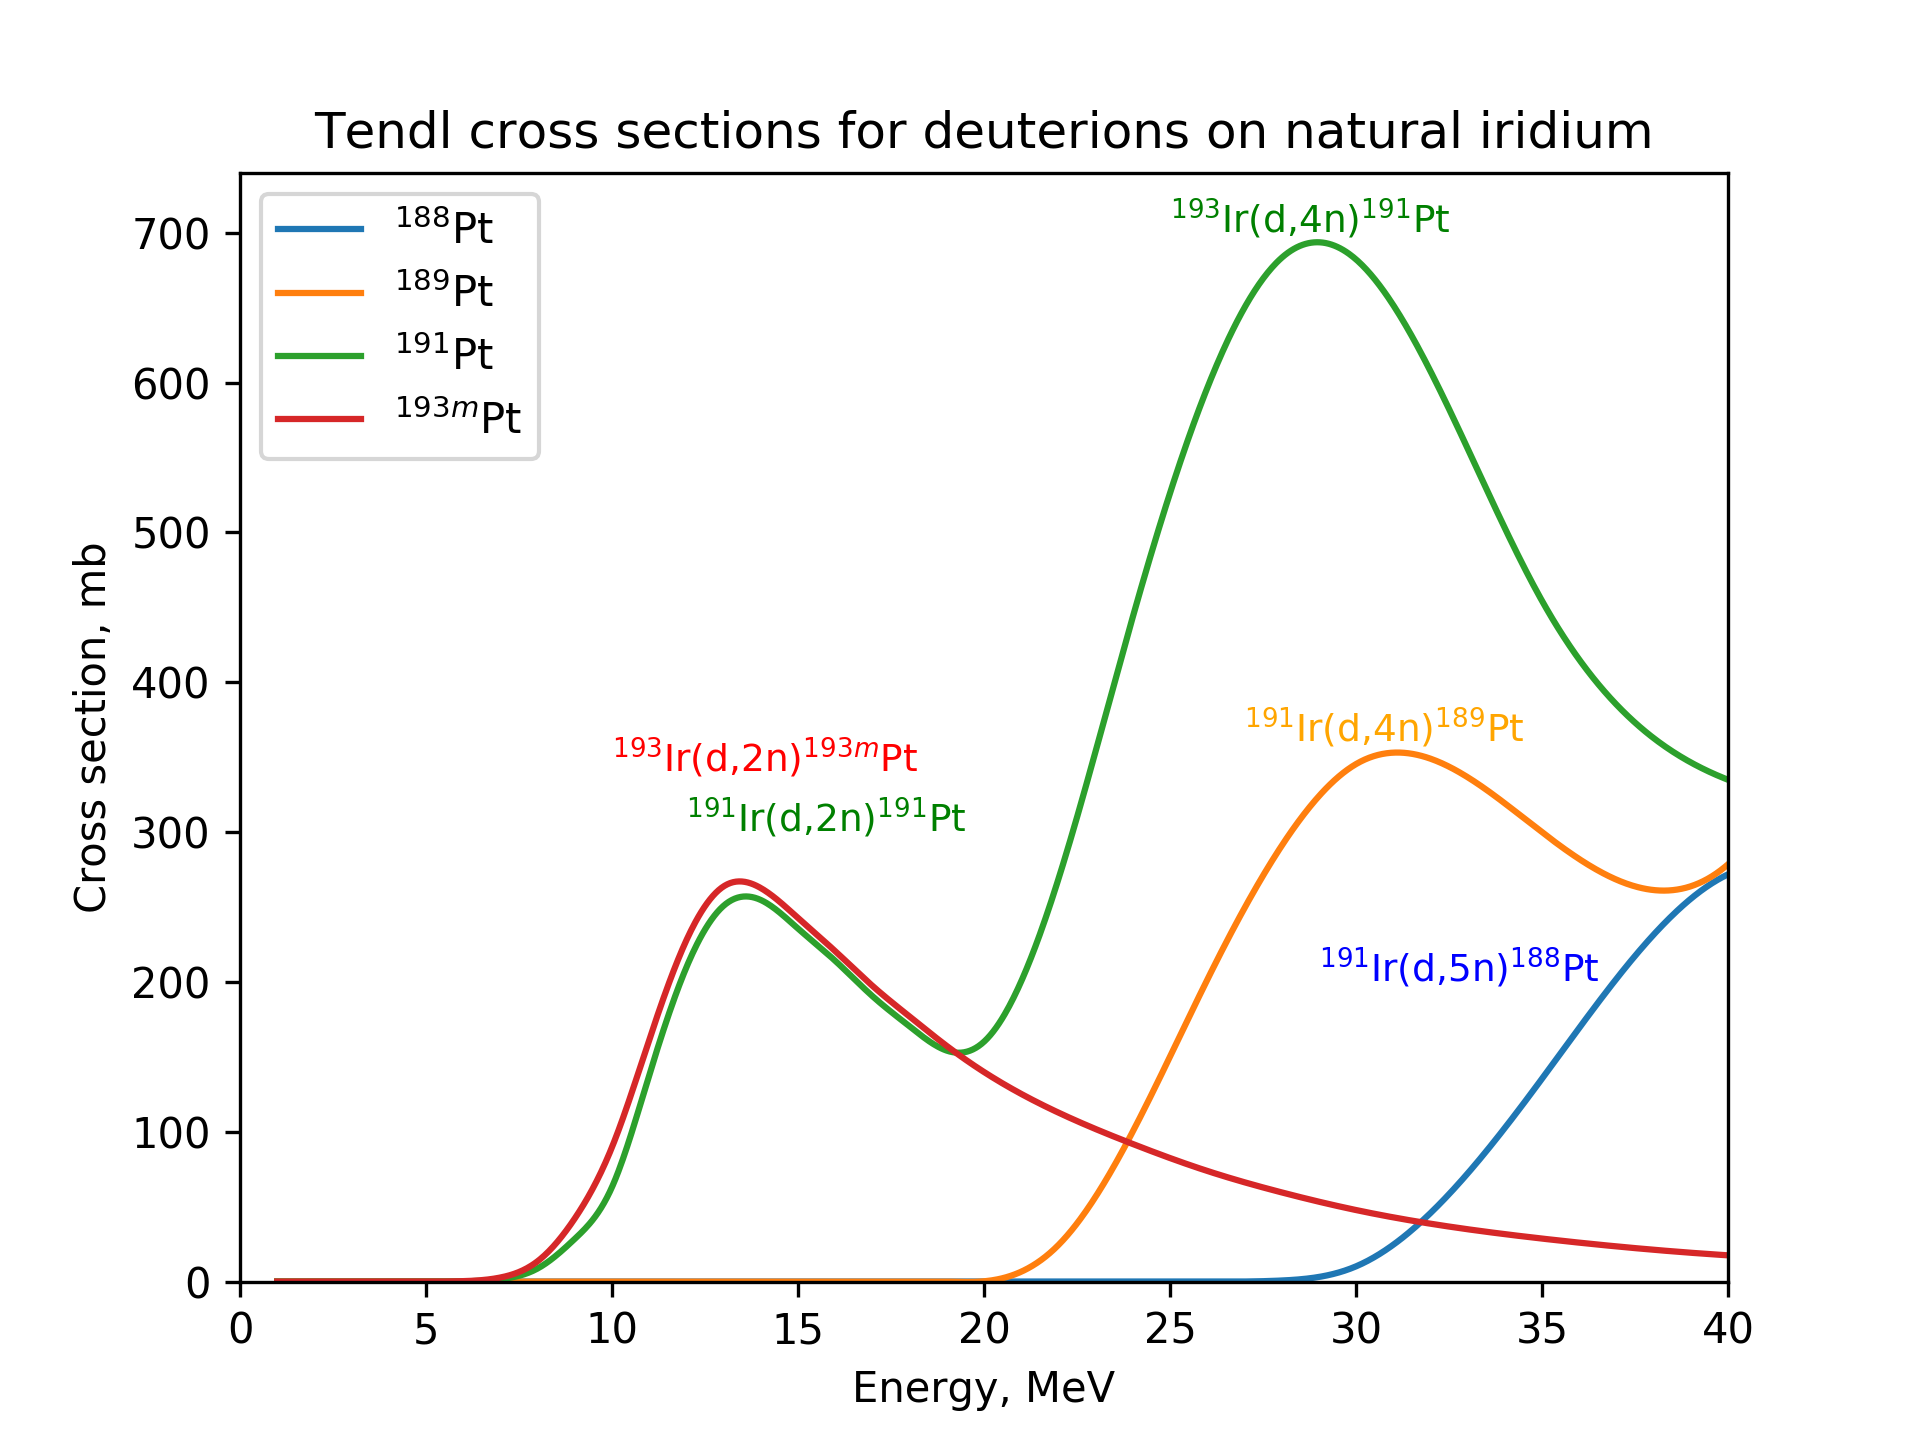
\includegraphics{Theory/reactionchannels_pt.png}
    \caption{Reaction cross sections provided by Tendl for the reactions $^\text{nat}$Ir(d,x)$^{188,189,191,193m}$Pt}
    \label{fig:pt_reactionchannels}
\end{figure}
\begin{comment}
\begin{figure}
    \centering
    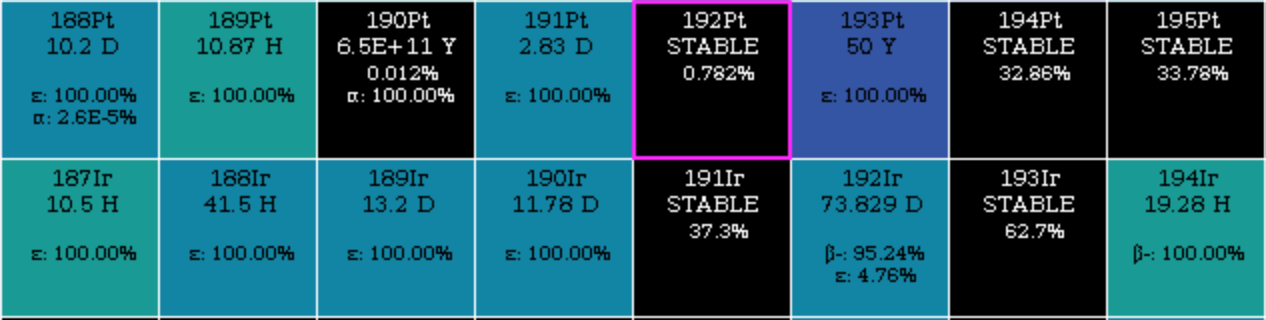
\includegraphics[width=12cm]{Ir(d)Pt.png}
    \caption{Nuclear chart for the platinum isotopes which can be produced from natural iridium }
    \label{fig:chart_irpt}
\end{figure}
\end{comment}


%\noindent A nuclear reaction
%The nucleus is built up on protons and neutrons, and these are bound through the strong nuclear force. 
\subsection{Constraints in nuclear reactions}
%\subsection{Energetic factors in nuclear reactions}

%\subsection{Dependence of }

%\noindent The binding energy depends on multiple parameters, which are based upon two models, the shell model and the liquid drop model (Krane, chapter 3.3, p. 68). The binding energy thus depends on the volume, which is constant throughout the nucleus, hence a volumeterm $a_V\cdot A$, a the surface of the nucleus which needs to be taken into account, since the nucleons on the surface is less tightly bound, $a_s\cdot A^{2/3}$. 
The potential energy of a nucleus is the sum of the attractive well from the strong nuclear force and the repulsive Coulomb barrier which acts repulsive between charged particles and the nucleus, acting long range (p. 152, Handbook of nuclear chemistry). The radius of the potential well is up to a few femtometer. For a positively charged particle induced nuclear reaction, the energy of the particle should exceed the barrier, or there will be an elastic scatter. However, there is a chance of tunneling, which drops with a factor 1/r where r is the distance from the center of the nucleus (Handbook of Nuclear Chemistry, chapter 3 - Nuclear Reactions, section, 3.2.3). The barrier also constraints the emission of particles for a decay channel of the compound nucleus, as the energy for an outgoing decay channel of positive particles must exceed the barrier. %There is also a centrifugal barrier, which is dependent on the orbital angular momentum of the the nucleus.  However, this barrier is more important in \textcolor{red}{direct reactions??}

The height of the Coulomb barrier is dependent on the radius and charge of the incoming or outgoing particle a and the target nucleus b.

\begin{equation}
    U_\text{Coulomb} = \frac{1}{4\pi \epsilon_0} \frac{e^2Z_a Z_b}{r_a + r_b}
\end{equation}

In addition, there is a centrifugal barrier, which can constraint some of the incoming particle energy in rotational energy, \textcolor{red}{which depends on the angular momentum of the incoming particle and and the nucleus???} (handbook of nuclear chemistry p. 155.)

\begin{equation}
    U_\text{centrifugal} = \frac{\hbar \ell (\ell+1)}{r^2}
\end{equation}

The sum of the barriers are the total barrier but the Coulomb barrier is the most important. 

%The orbital angular momentum is dependent on the mass and energy of the particle, but also the impact parameter of the reaction, which is the "distance" between the projectile and the nucleus

%\begin{equation}
%    \ell\hbar = (mv)b, \quad b\leq r_a + r_X
%\end{equation}

%\noindent where $r_a$ and $r_X$ are the radii of projectile and target nucleus. If $\ell=0$, the impact parameter is zero. If $\ell\neq 0$, then some of the energy of the projectile will go to rotational energy of the nucleus (Handbook of Nuclear Chemistry, chapter 3 - Nuclear Reactions, section, 3.2.4). The probability of this drops with $1/r^2$, and if the impact parameter is large, this will constraint some of the energy that would have gone to the nuclear reaction. Figure \ref{fig:sumOfPotentials} shows an overview of the various potentials; centrifugal barrier, Coulomb barrier and nuclear potential. The figure is for $^{58}$Zn, but the figure is only an example. \textcolor{red}{maybe make figure self?}. 


\begin{figure}
    \centering
    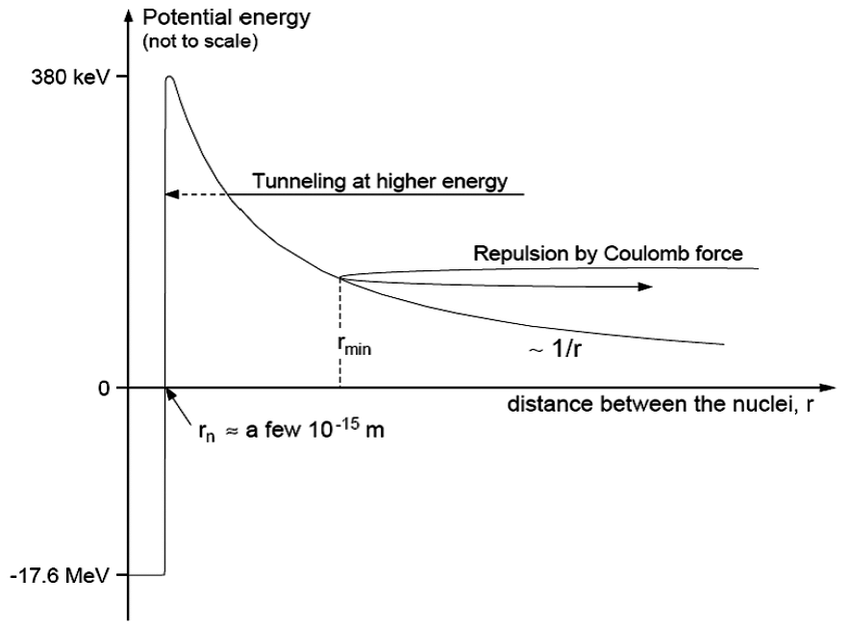
\includegraphics[width=8cm]{Theory/Coulomb_barr.png}
    \caption{ }
    \label{fig:Coulomb_barrier}
\end{figure}



\begin{comment}
\noindent The separation energy is the energy required to remove a particle from the nucleus. That is the difference in the binding energy for the two nuclei. The neutron separation energy is 
\begin{equation}
    S_n = B(^A_z X_n)-B(^{A-1}_z X_{n-1}) = c^2(m(X^{A-1}_zX_n)-()
\end{equation}\\ 
\end{comment}

\noindent In a nuclear reaction, the mass-energy is conserved, which is denoted as the Q-value. The reaction Q-value is the difference is masses between before and after the nuclear reaction occurred (Krane, chapter 11.2). It is defined as 

\begin{equation} \label{eq:Q_value}
    Q = (m_i - m_f)c^2 = (m_X + m_a - m_Y - m_b)c^2
\end{equation}

\noindent where $m_i$ is the initial mass, $m_f$ is the final mass and c is the speed of light. If $Q>0$, then the reaction is exoergic, which means that energy is released in the reaction. There is no threshold energy of the projectile required for the reaction to occur, if only the projectile is present the reaction can occur. If $Q<0$, then the reaction is endoergic, which means that the kinetic energy of the incoming projectile is converted into nuclear mass or binding energy. For endoergic reactions to occur, there is a minimum threshold energy of the projectile in order for the reaction to happen, which is defined as (Krane, 11.2, p. 382)

\begin{equation} \label{eq:reaction_threshold}
    E_\text{threshold} = (-Q) \cdot \frac{m_Y +m_b}{m_Y + m_b -m_a}
\end{equation}


\noindent The energy threshold thus depend on the Q-value, the Coulomb barrier for charged particles, and the centrifugal barrier if angular momentum $\ell\neq 0$. The parity though depend, even numbers of $\ell$ mix with even, and odd with odd (Handbook of Nuclear Chemistry, chapter 3Nuclear Reactions, section, 3.2.3). This gives an indication on when a reaction can energetically occur, but does not tell us how probable the reaction is. %Equation \ref{eq:reaction_threshold} indicates that a higher mass for the particle in the outgoing channel $m_b$, will lower the energy threshold.\\ 

%The nuclear binding energy is a number which tells us how tightly bound the nucleus is, and how much energy is required to separate nucleons from the nucleus. The nuclear binding energy is related to the mass of the nucleus, through the famous equation   E=mc^2

The binding energy is the mass-difference between the nucleus as a whole, and the number of protons and neutrons added
\begin{equation} \label{eq:Binding_energy1}
    B = c^2(z\cdot m_p + n \cdot m_n - m_N)
\end{equation}
\noindent where z is the number of protons, n is the number of neutrons, $m_p$ is the proton mass, $m_n$ is the neutron mass, $M_N$ is the mass of of the nuclide, which is the number of nucleons A minus the number of electrons, $M_P = m_A - z\cdot m_e$ (the electronic binding energy per electron is excluded). From Krane's derivation of the nuclear binding energy (Krane, chapter 3.3, p. 65). 

From equation \ref{eq:Q_value}, the larger the mass of the outgoing decay channel, the more negative the Q-value will be. Protons (+1 charge) and neutrons (neutral) are the simplest decay channels of the compound nucleus, each carry a spin of $1/2$, with masses $m_p=938.28$ MeV/c$^2$, and $m_n=939.57$ MeV/c$^2$. Combinations like deuterons (d=1p+1n, charge +1) has a mass difference of $\Delta=$2.2 MeV/$c^2$ from realising 1 proton and 1 neutron separately, a triton (t=2n+1p, charge +1) with $\Delta=8.5$ MeV/$c^2$,  3-Helium ($^{3}$He=1n+2p, charge +2) with $\Delta=7.7$ MeV/$c^2$ and alpha-particle ($\alpha$=2n+2p, charge +2) with $\Delta=28.3$ MeV/c$^2$. Thus, Q-values are higher in value, the lighter the particle is. However, in this work, we can clearly see that protons, neutrons and alpha-particles are strongly fed decay channels, while the other don't even appear. The suggested reason for this is that due to \textcolor{red}{blablabla nuclear physics stuff, like shell structure}, protons and neutrons are favoured, but since the alpha-particle has such a large binding energy, this channel is also favoured.  

\subsection{Deuterons and stopping power}

The deuteron consists of a neutron and a proton, and is the simplest bound state of nucleons. Nucleons have an average binding energy per nucleon of 8 MeV. The detuteron with an observed mass value of 2.224 MeV (Krane, p. 81) is a weakly bound. Thus little energy required to break up the deuteron. \textcolor{red}{does this affect?}

The stopping power of a deuteron beam running through forms the Anderson \& Ziegler. \textcolor{red}{write about Anderson and Ziegler. And how does the stopping power give a flux??}


(Techinque nuclear and particle physics p. 30-31):  
For a particle beam the energy loss is not a continuous process, but collisions based on statistics. A measurement of identical particles will thus show a statistical distribution of ranges centered about the same mean value. This is called range straggeling \textcolor{red}{this part relevant for describing Ziegler flux?}. 

Energy straggling: the energy loss distribution: (instrumentation p. 49)
"For any given particle however, the energy lost will not be equal to this mean value because of statistical fluctuations which occur in the number of collisions suffered and in the energy transferred in each collision. An initially monoenergetic beam will therefor show a distribution of energy rather than a delta function peak shifted down by the mean energy loss given by the dE/dx formula after passing through a fixed thickness of material.. see if more necessary?"

\begin{comment}
Range: How far will particles penetrate before they lose all there energy. Moreover, if assume that the energy loss is continous, this distance must be a well defined number, the same for alll identical particles with the same initial energy in the same type of material. This quality is called the range of the particle, and depends on the type of material, the particle and its energy. Experimentally the range can be determined by passing a beam of particles at the desired energy through different thicknesses of the material in question and measuring the ratio of transmitted to incident particles. For small thicknesses all the particles manage to pass through. As the range is approached this ratio drops. The surprising thing however is that the ratio does not drop immediately to the background level as expected of a well defined quantity. Instead the curve slopes down over a certain spread of thicknesses. This result is due to the fact that the energy loss is not continous, but statistical in nature. Indeed two identical particles with the same iniitial energy will not in general suffer the same number of collisions and hence the same energy loss. A measurement with an ensemble of identical particles therefor will show a statistical distribution of ranges cented about same mean value. This phenomenon is known as range straggling. In a first approximation this distribution is Gaussian in form. The mean value of the the distribution is known as the mean range and correspond to the midpoint of the corresponding slope. This is the thickness at which roughly half of the particles are absorbed. More commonly however what is desired is the thickness at which all the particles are absorbed, in  which case the in which case the point at which the curve drops to the background level should be taken.  This point is usually the tagent to the curve at the midpoint and extrapolating to the zero level. This value is known as the extrapolated or practical range
\end{comment}


\section{Nuclear reaction models}

The optical model (proton/neutron, and alpha/deuteron), gamma strength function. 

\subsubsection{EMPIRE 3.2.3}
\subsubsection{CoH 3.5.3}
\subsubsection{ALICE 2017}
\subsubsection{TALYS 1.9}
\subsubsection{TENDL 2019}



%, the equal number of protons and neutrons make up $z\cdot^1H$, thus we can rewrite equation \ref{eq:Binding_energy1} to 

%\begin{equation}
%    B = z\cdot m_{^{1}H} + n\cdot m_n - m_{A}
%\end{equation}

%\noindent 
%Separation energy of a particle is the energy required to be removed from the nucleus. This is defined as the difference in binding energy between the nucleus with the particle and the nucleus without the emitted particle. Since heaavier particles such as tritrium has a lower binding energy, more energetically easy to separate. n and p require more. 



\begin{comment}

\subsection{Nuclear cross sections}

The cross section for a reaction can be divided into the cross section of the formation of the compound nucleus via interaction with the incoming projectile a, and the probability that the compound nucleus decay by decay channel b. The total reaction cross section is thus the sum of all the different reaction channels, 
\begin{equation}
    \sigma = \sum_b \sigma(a,b)
\end{equation}
where b can be multiple particles. The general equation which is used to calculate cross sections in this experiment is the following equation, which is solved from equation \ref{eq:activity_eob} (referenced to in the later parts of the paper)

\begin{equation} \label{eq:cross_section_equation}
    \sigma(E)=\frac{A_0}{N_T\Phi(E)(1-e^{-\lambda \Delta t_\text{irr}})}
\end{equation}

not, need to check if this is the correct one.. 
\begin{equation}
    \sigma(E) = \frac{A_0 \cdot t_\text{irr}}{N_T \cdot \Phi(E)(1-e^{-\lambda t_\text{irr}})}
\end{equation}
\noindent where $A_0$ is the end of beam activity of the resulting product nucleus (Y), $t_\text{irr}$ is the irradiation time, $N_T$ is the number of target nuclei (X), $\Phi(E)$ is the projectile flux (a), and $\lambda$ is the decay constant of the product nucleus. 

\newpage

Why we are interested, why is there a need for nuclear production cross sections. 



The Q-value for nuclear reactions 

Compound nucleus, what happens. 
Q value, binding energy, particle emission, probabilities (why does n, p/alpha emission require higher energy, but is more favoured than T emission if both possible.)


\subsection{Expected products from deuterions on iridium, iron, cupper and nc}

Include figure of different nuclear charts, and write about Q values, and reaction channels, which makes it more probable that we observe it (eg. when neutron, proton/alpha channels opens).





\section{From book}

In a nuclear reaction, the energy, linear momentum, the total number of protons and neutrons, angular momentum and conservation of parity is conserved. \\

The compound nucleus; the collisions are described by a model called Multistep Compound Model (Feshback, Kerman and Koonin, 1980), which is the model that reaction modeling code EMPIRE and TALYS rely on. \textcolor{red}{find out what ALICE does ???}

Products of a nuclear reaction can be anything than conserve the various variables. Mass energy conservation is the Q-value, which is the mass differene in the reactant nuclei (projectile and target in this case) and product nuclei (decay channel particles and product). Binding energy (nuclear mass energy) often denoted as $\Delta=(M_0 - Au)c^2$, where A is atomic mass number, u is atomic mass unit. Q-value can be rewritten: 
\begin{equation}
    Q = \Delta_\text{projectile} + \Delta_\text{target} - \sum \Delta_\text{products}
\end{equation}

Charged particle reactions with heavy nuclei which is the case here, can have positive or negative Q-value. If the Q-value is negative, energy is required to induce the reaction. The reaction is negative if the sum of products is less than the sum of reactants. The excitation energy of the product nucleus is the extra energy which is deposited in the product nucleus. The decay of this is often times $\gamma$-rays (?). If the excitation energy is lower than the binding energy of the nucleus?  Threshold is the minimum energy required for the incoming projectile to form a product nucleus, which is then in its ground state. 

\begin{equation}
    \text{mass-energy}: \quad \Delta_t+ \Delta_p + E_p 
\end{equation}




\section{The decay of the compound nucleus}
At the energy ranges in which this work is operating in, the nuclear reaction is caused by a fusion between the incoming projectile to create an highly excited compound nucleus. \\ 

\noindent 
The decay favoured decay channel is dependent on multiple properties such as the charge and angular momentum. The coulomb potential is defined as 

\begin{equation}
    U_{c} = K\frac{z_1 z_ 2 e^2}{A_1^{1/3} + A_2^{1/3}}
\end{equation}

where z is the the number of charges, e is the electrical charge and $A^{1/3}$ is the nuclear radius which is equal to $r=r_0 A^{1/3}$. K is a constant value. 

The centrifugal barrier (which is the amount of energy which is conserved in rotational energy) depends on the angular momentum 

\begin{equation}
    U_{s} = \frac{\hbar \ell(\ell+1)}{2\mu r^2}
\end{equation}

where $\mu$ is the reduced mass $u\cdot \frac{A_1 A_2}{A_1 + A_2}$. 


\textcolor{red}{Table \ref{tab:decaychannel_particles} might be wrong in the sense $J^\pi$. Might just be the total spin which is of interest? But since $J=l+s$, the spin will give a higher intrinsic angular momentum. Since $|I_i - I_f| \leq \ell \neq I_i+I_f$, $\ell$ can be multiple values, and the parity is thus dependent on the value here. (Krane, chapter 8.5, p. 257). The centrifugal potential is thus} 

\begin{equation}
   U_{0,s} =  \frac{\ell (\ell +1)\hbar}{2mr^2}
\end{equation}

and the Coulomb potential is

\begin{equation}
    U_{0,c} = K\frac{z_1 z_2 e^2}{A_1{1/3}+ A_2^{1/3}}
\end{equation}

The 

\begin{table}[]
    \centering
    \caption{The table shows the most common decay channels for the decay routes available in this energy region. $\Delta$ is the binding energy of the alpha particle, which can be calculated using equation \ref{eq:Binding_energy1}, where the mass of the proton is $m_p = 938.28$ MeV/c$^2$ and $m_n=939.57$ MeV/c$^2$. $\Delta$ is thus the difference in in energy-mass between the particle composed of protons and or neutrons, and a equal number of protons and neutrons independent. All parities are positive due to angular momentum $\ell=0$.  }
    \begin{tabular}{|c|c|c|c|c|}
         \hline 
         Particle & \Delta (MeV) &J^\pi & Charge \\
         \hline
         p & - & $\frac{1}{2}^+$ & +1 \\
         n & - & $\frac{1}{2}^+$ & 0 \\
         d & 2.2 & $1^+$ & +1 \\
         t & 8.5 & $\frac{1}{2}^+$ & +1 \\
         ^{3}He & 7.7 & $\frac{1}{2}^+$ & +2 \\
        \alpha & 28.3 & 0^+ & +2 \\
        \hline
    \end{tabular}
    \label{tab:decaychannel_particles}
\end{table}


\begin{table}[]
    \centering
    \begin{tabular}{|c|c|c|c|c|c|c|}
        \hline
        Target & Proton & neutron & deuterion & triton & ^{3}H & \alpha  \\
        \hline
        Fe (Z=26) & & & & & &  \\
        Ni (Z=28) & & & & & &  \\
        Cu (Z=29) & & & & & &  \\
        Ir (Z=30) & & & & & &  \\
        
    \end{tabular}
    \caption{The Coulomb barrier in MeV for each of the targets. Can be used to explain why we see what we see. }
    \label{tab:my_label}
\end{table}

The total angular momentum J is the sum of the orbital and intrinsic angular momentum (spin), thus 
\begin{equation}
    \mathbf{J} = \mathbf{\ell} + \mathbf{s} 
\end{equation}

The spin is the sum of unpaired paired protons and neutrons. The total nuclear spin is thus $I = \sum_i J_i$.  The value of the angular momentum is
\begin{equation}
    |I_i - I_f| \leq \ell \geq |I_i + I_f|
\end{equation}

Thus, 





\end{comment}


%\section{Radioactive decay law and Gamma-ray spectroscopy}
\section{Detection and identification of radionuclides}
Gamma-ray spectroscopy is a method to identify and obtain information about radioactive nuclei present in a detector. As beta and alpha decay can result in an excited daughter product, the spectrum in fact shows the de-excitation of the daugher product. Since we know that these gamma-lines are transitions which happens right after a beta or alpha decay (or isomer transition), we identify the parent with gamma-ray spectroscopy. A detector has channels in which counts are regiserted. These channels are ... similar to the gamma-ray energy. Thus a spectrum has channels (which increases in energy) along the x-axis and and counts along the y-axis. If a detector registers many counts, it means that the state is highly populated, and the intensity of the gamma is strong (Krane, p. 351). 



\subsection{High purity Germanium detector}
High purity Germanium detector is a type of semiconductor, which is a material where the energy required to remove an electron from the valence band (in the outer atomic shell) to the conduction band is small. The germanium atom has atomic number 32, and 4 valence electrons in the outer p4 shell (need citation?). The atoms in the detector are bound through covalent bonds in a crystal structure. The main mechanism of a semiconductor is creation of electron-hole pairs after energy deposition of an ionizing particle in the crystal. If an electron is excited to the conduction band, a hole is left. This hole can move as a neighboring electron fills this spot, and it can cause a chain reaction, and the hole will move in the crystal. Both the electron in the conduction band and the  and the hole in the valence band contributes to an electric current. Under influence of an electricfield, the electron-hole pairs will be collected and we can measure the incident as a count. The major
advantage with semiconductor detector is that the average energy to create an electron-hole pair is
very low, which results in a superior energy resolution in comparison to other detectors like gas and
scintillation detectors. High energy resolution advantageous in gamma-ray spectroscopy which makes
it possible to separate to gamma-ray peaks within less than a keV. At room temperature, thermal
energy can excite the electron from the valence to the conduction band and cause noise in spectra.
Therefor, Germanium detectors are operated at 0 Kelvin. Write about recombination and trapping,
noise, np semiconductor junction, depletion depth?? (Techniques for Nuclear and Particle Physics Experiments, William R. Leo, p. 215-216). 


%\subsection{Obtaining a gamma-rey spectrum}
Ideally, for all gamma-rays with the same energy, should be detected in the same channel giving a step function. However, realistically, the resolution of a detector is not that good, and instead of seeing a delta peak, the peak is typically gaussiam shape with a finite width. The full width half maximum $\Delta E$ of the peak tells us how well the relative resolution at gamma-energy E,
\begin{equation}
    \text{resolution} = \frac{\Delta E}{E}
\end{equation}

The energy resolution is important, as it tells us how well it can distinguish two close lying peaks from each other (Techniques of Nuclear and particle Physics.. , p. 117).  The resolution of a germanium detector very good (0.1\% for a 1 MeV gamma-ray) in comparison to for instance NaI detector (8-9\% for a 1 MeV gamma-ray) (Techniques of Nuclear and particle Physics.. , p. 117). \textcolor{red}{explain why, prob in semiconductor chapter!} \\


The peak it self is not directly gaussian. Ionizing radiation statistics is based upon Poisson statistics, where  and the probability of observing N events is a discrete value

\begin{equation}
    P(N) = \frac{\mu^N e^{-\mu}}{N!}
\end{equation}

where $\mu$ is the mean value. This distribution counts when the probabiliy is a small (eg decay prob?) value and that the total number of trials are large (number of decays) (Techniques of Nuclear and particle Physics.. , p. 85).  For poisson distribution, the average is equal to the variance; $\sigma^2=\mu$. From there, the standard deviation ($\sigma$) is thus equal to the squareroot of the average. 

The distribution is not symmetric, but as $\mu$ increases in value, the peak approxes a gaussian shape. The total number of counts is the area of the peak. The total peak is a Guassian assumption but with an exponential skew towards kiw E caused by incomplete charge collection, abd a step function for taking compton backgroun into account. 

In calculation of the peak area, there are two uncertainties of relevance, the relative statistical uncertainty in the counting from the Poisson statistics, 
\begin{equation}
\sigma N_i = \sqrt{N_i}
\end{equation}

If numb of counts $N_i =10000$, the relative uncertainty ($\frac{\sigma N_i }{N_i}= \frac{1}{{sqrt{N_i}}}$=1\%). Therefor we say that a good number of counts is 10000 or more to reduce the statistical uncertainty. The other is systematic in the detector, and can for instance be due to a process called annealing, which is heat damage to the detector. Can fix by taking a blanket of resistor wrap crystal in, rise to high temp, let it sit and slowly deheat to room temp, traps will defuse and detector is repaired (this is notes from Andrew).

Also write about deadtime! 
\subsection{Gamma-ray spectrum}

Spectrum: consists of photopeaks, a compton continuum, compton edge, backscatter peak, single exscape double escape. In cases where positrons exist, chances of having a broad fat 511 keV peak. 

Germanium detecors, highest resolution for gamma-rays, from frew keV to 10 MeV. The peak to Compton ratio is much greater due to the higher photoelectric cross section of Germnaium . The largets challenges are with signal to noise ratio, it is important to shield very well to minimze background radiation (Techniques for Nuclear and particle..... William R. Leo, p. 241). \\ \\

\noindent 
here from another citation: "Practical Gamma-ray Spectroscopy". Gordon R. Gilmore. Nuclear Training Services Ltd Warrington UK. \textcolor{red}{(can be find under articles in masterthesis). This book can also be used in particle interaction in matter check!!}
In a detector, the particles interacts as the photons described in particle interaction, via photoelectric, compton scattering and pair production. Photoelectric absorption where the photon is completely absorbed by atomic electron is desired because all of the energy is deposited within the detector. For a compton scattering event, if the resulting photon's energy is also deposited in the detector (for a large detector), then the total energy would add up. Same for pair production. The photon must interact in the detector volume, and the resulting electron and positron energy is deposited in the detector volume. However when the positron slows down, it annihilates with one atomic electron, releasing two 511 keV photons. If both annihilation photons's energy is deposited in the detector volume this will also contribute to a full width peak. If one 511 photon escape and the other is deposited, there will be a peak at $E_\gamma-511$ keV, and if both peaks escape, there will a double escape peak at $E_\gamma-1022$ keV. The "degree of incomplete absorption" depends upon the size of the detector and the gamma-ray energy. As previously discussed photoelectic effect dominates at low energies, and the less compton scattering and of course pair production (for E gamma higher than the threshold.). The detector size also matters because the larger the more room for the photon to scatter in and lose energy before escaping. (p. 32) \\

The total spectrum can be seen on p. 33 in the book. Pile-up is done because of random summing, determined by the statistical probability of two gamma-rays being detected at the same time and therefor on the sample count rate. 

Interaction with detector shielding: Photoelectric effect can be followed by emission of characteristic X-ray of the absorbing medium. X ray can escape the shielding and be deteced by the detector. Compton scattering: most gamma rays are scattered through the a large angle by the shielding, BACKSCATTERED. Whatever the initial enervy  was (if scattered by more than 120 degrees) are within 200-300 keV. Peak appears as broad. Pair production: annihilation peak (511 peak) caused by the escape of one of the 511 keV photons from the shielding following annihilation of the pair production positron. Analogous to the single and double escape mechanisms within the detector but only on 511 keV photons can ever be detected since they are emitted in the opposit direction. So in order to have a 511 peak, energy of gamma ray must be more than 1022 keV. (p. 34-35).

The 511 peak can also be expected when postron emitters are present since beta + particle interacts with electron.  

Since Compton scattering can be in a spectrum of energies, the gives rise to a Compton continuum, before the gamma-ray escapes the detector. 


The shape of the peak: The peak is a histogram that approximate a Gauss curve (p. 186). Peak searching (SAMPO) using first and second order derivatives to search for peaks (p.185)
Due to incomplete charge collection (that electron or holes are not collected) no matter how caused moves counts from the centre of the Gaussian distribution to lower channels, creating a low energy tale to the peak (p.135).  

\textcolor{red}{Include a picture of peak shape and gamma-ray spectrum!! from the same book}

\chapter{Experimental setup}

The thin foil stacked-target technique was applied to measure the experimental cross sections for reactions induced in iridium, iron, nickel and copper with deuteron energies ranging from ca. 33-5 MeV. This method is well-described in literature \footnote{https://sci-hub.tw/https://doi.org/10.1016/j.nimb.2016.09.018}\footnote{Niobium paper and iron paper from Andrew} for protons. This is however the first experiment using deuterons and the results may differ as for instance the deuteron break up effect is unknown. 

\section{Lawrence Berkeley National Laboratory's 88" Cyclotron}

Lawrence Berkeley National Laboratory (LBNL) is a national research laboratory on behalf of the U.S. Department of Energy through its Office of Science, and is operated by University of California, Berkeley. LBNL was founded by Ernest Orlando Lawrence, the inventor of the cyclotron \footnote{https://www.lbl.gov/about/}. \\ 


\noindent
The 88" Cyclotron has many purposes, and can accelerate both light and heavy ions up to Uranium, with a cyclotron number K=140  \footnote{http://cyclotron.lbl.gov/home}. %The cyclotron number is the maximum kinetic energy which can be reached for protons (with no relativistic factors taken into account). The maximum kinetic energy a particle can gain is found from the cyclotron number:

%\begin{equation}
%    \frac{E_k}{A}=K\Big(\frac{Q}{A}\Big)^2
%\end{equation}
\noindent 
%For deuterons with mass number A=2 and charge Q=1, the maximum kinetic energy is $E_k=70$ MeV. 
There are multiple programs that takes place in the facility\footnote{https://ieeexplore.ieee.org/abstract/document/7999622/authors#authors}; chip testing and space effects testing, super heavy element searches, fundamental nuclear structure measurements, novel scintillation characterization, fission yield and neutron inelastic scattering measurements (GENESIS) (from Andrew). \\

\noindent 
A cyclotron is a device that accelerates positively charged particles. It is operated by an alternating electric field, and a perpendicular magnetic field, which by the Lorentz Force forces the particle to accelerate in an outward spiral. 
The facility is figured in figure \ref{fig:LBNL_88}, which consists of a cyclotron vault, and experimental caves in which the beam can be bent to with bending magnets. Faraday cups (not in figure) can measure the beam current at different steps along the tube, which makes it possible to measure the transition efficiency of the beam. Faraday cups are dense metal block, usually 6-7 cm broad Copper and Tantilum. It works as a beam stopper, and can be lowered into the beam line to measure the current. It is electrically isolated, which makes it possible to measure the current, since we know the number of initial particles accelerated. Due to electrons close to surface might be scattered of, it can read of higher positive charge than what is correct. Therefor, a magnet surrounds the cup to bend the electrons back to the Faraday cup in what is called magnetic suppression. Cave 0 is used mainly for neutron beam, chemistry, and isotope production, and was used for irradiation of the target stack.


\begin{figure}
    \centering
    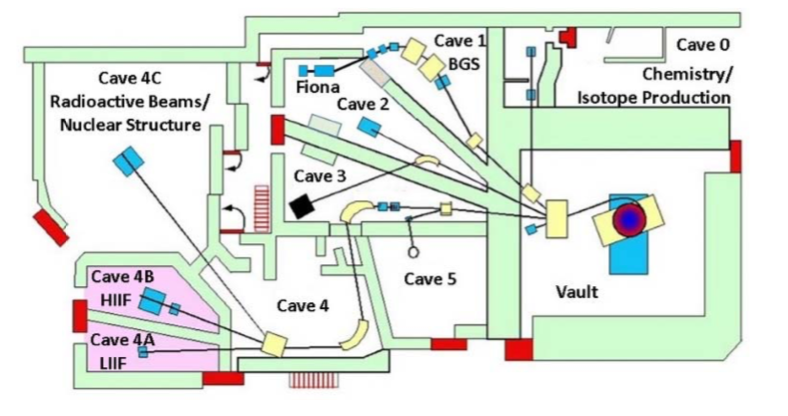
\includegraphics[width=0.8\textwidth]{Experiment/LBL_88.png}
    \caption{An overview of the 88" Cyclotron facility. https://cpb-us-e1.wpmucdn.com/sites.usc.edu/dist/7/89/files/2018/04/133-18q03um.pdf }
    \label{fig:LBNL_88}
\end{figure}

\section{The experiment}
The main motivation of this experiment was to measure production cross sections of the products produced after irradiation of a stack of thin iridium foils along with thin monitor foils Nickel, Cupper and Iron foils, with a 33 MeV incident deuteron beam, as shown in figure \ref{fig:experiment_illustration}. 
\begin{figure}
    \centering
    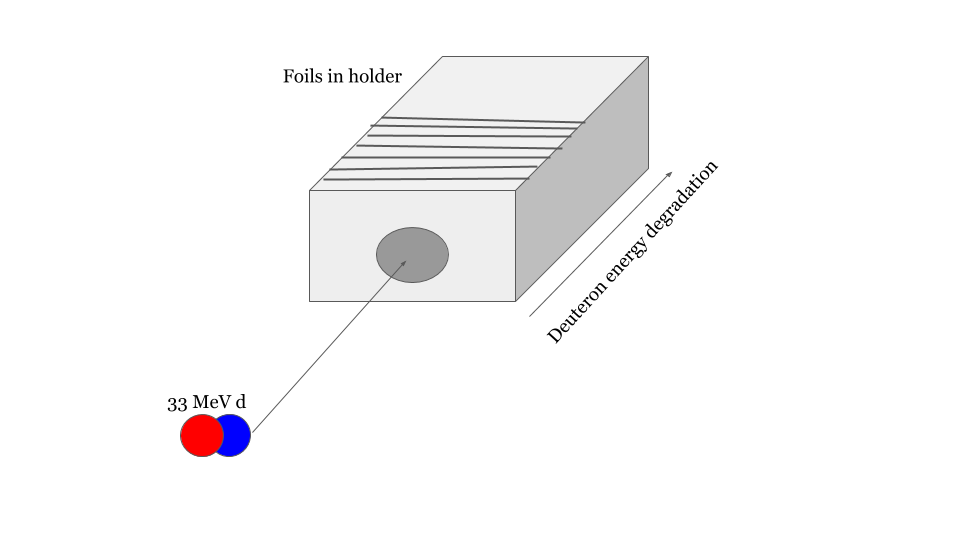
\includegraphics[width=0.7\textwidth]{Experiment/Illustration_beamOnTarget.png}
    \caption{The fundamental idea of the experiment where a stack of targets are placed in a target holder, and irradiated with accelerated 33 MeV deuterons. As the energy degrades through the beam stack, it is possible to have multiple cross section measurements at different energies.}
    \label{fig:experiment_illustration}
\end{figure}

The beam was ca. 1 cm in diameter, and with each target foil being ca. 25 by 25 mm, the beam was underfilled. As the energy was degraded through the stack, multiple cross sections at different energies were possible to measure for the different induced reactions. For production cross section data experiments, thin targets (foils) are used, in the other of a few $\mu$m \footnote{(Syed M. Qaim. Nuclear data for production and medical application of radionuclides:
Present status and future needs. Nuclear Medicine and Biology, 44:31–49, jan 2017.)} are used, since the induced activity is low, meaning that the deadtime of the detector and the dose to human will be low.  

\noindent 
%From equation \ref{eq:activity_eob}, the cross section as a function of energy is 

%\begin{equation} \label{eq:experimental_CS}
%    \sigma(E)=\frac{A_0}{N_T \Phi (1-e^{-\lambda \Delta t_\text{irr}})}
%\end{equation}

\noindent 
%where E is the average energy across the foil (MeV), $A_0$ is the end of beam activity (Bq), $N_T$ is the number of target nuclei, $\Phi$ is the beam current (nA), $\lambda$ is the decay constant of the nucleus ($s^{-1}$) and $\Delta t_\text{irr}$ is the irradiation length (s). 

\noindent 
Equation \ref{eq:cross_section_equation} is the equation which is used in the calculation of the cross sections. In order to calculate the cross section of a product, end of beam activity, number of target nuclei and beam current must be found, where for the end of beam activity, the detector efficiency need to be estimated. The number of target nuclei was estimated through characterization of the foils. $A_0$ was estimated using equation \ref{eq:Final_Expression_A0}, which depends on the efficiency calibration of the detectors as a function of gamma-ray energy, the number of counts registered and the intensity of the gamma-rays emitted by the source, the decay constant of the source and the delay time. Some of the nickel, copper and iron deuteron-induced cross section are well-established, and can  be used to determine the beam current throughout the stack. 



%The end of beam activity goes into the equation, which is given in equation \ref{eq:Final_Expression_A}. The activity from spectra measured at different delay times after end of beam can be found, with respect to number of counts, efficiency of detector, intensity of gamma-rays, the decay constant of the nucleus $\lambda$ and the counting time $\Delta t_c$. As we know that radioactive decay curves follows equation \ref{eq:ndecay_chains}, and dependent on how many step the decaychain consists of, the end of beam activity can be estimated by extrapolating backwards in time with a curve fit. \\

%\noindent 


\subsection{Target design and foil characterization}
\textcolor{red}{why was the order what it was??}
In this experiment, the target stack was composed of of ten natural iridium foils (99.9\%) foils, along with ten natural nickel foils (..\%), ten natural copper foils (..\%) and three natural iron foils (..\%) (from Goodfellow Corporation, Corapolis, PA 15108, USA) serving as monitor foils. Along with two stainless steel foils in the front and the back of the stack, a proton degrader (a 6061 aluminum alloy), and an extra nickel neutron monitor foil was used to obtain production cross sections at multiple energies, using one incident deuteron beam. The full order of the stack and the characterization of each foil can be seen in table \ref{table:foil_characterization}. \\

\noindent 
Each foil were cut into approximately 25 by 25 mm squares, and each foil was characterized using a caliper (Mitutoyo Absolute Digimatic) to measure the length across each side, a gauge caliper (Mitutoyo IP65 Coolant Proof) to measure the thickness and an analytical balance weight (Mettler Toledo) to measure the mass of each foil which was prewashed with isopropanol. For each measurement, the unit was measured 4 times, and the values listed in table \ref{table:foil_characterization} are averaged values. The length and mass were used to measure the mass density. The thickness was not used in the
calculation of the mass density, but was a good indication that the foil thicknesses were consistent.
\textcolor{red}{For underfilled beams, the mass density of the foil is used to find the number of nuclei per cm$^2$, by using the area of each foil.} The mass density was calculated using the mass of each foil divided by the area
\begin{equation}
    \rho \Delta r = \frac{m}{A}
\end{equation}

\noindent 
The uncertainty in each parameter was calculated using the standard deviation (equation \ref{eq:standard_dev}) of the four measurements per unit, and the total uncertainty was calculated using the approximation of uncorrelated variables used in equation \ref{eq:uncertainty_simplification}. The conversion from mg per cm$^2$ to nuclei per cm$^2$ was done numerically, by multiplying the mass density with Avogadro's number $N_A$ and dividing by the mol-mass of the target atoms. \\

\noindent 
After the characterization, each foil was mounted on a plastic frame with an open space in the middle and attached with capton tape along the edges (from previous experiments, capton tape have shown to be be a large \textcolor{red}{proton?} degrader, so it was important that the tape was not in the beamline \textcolor{red}{cite Article by Andrew}). The target frames can be seen in figure \ref{fig:targets_on_frame}. 

\begin{figure}
    \centering
    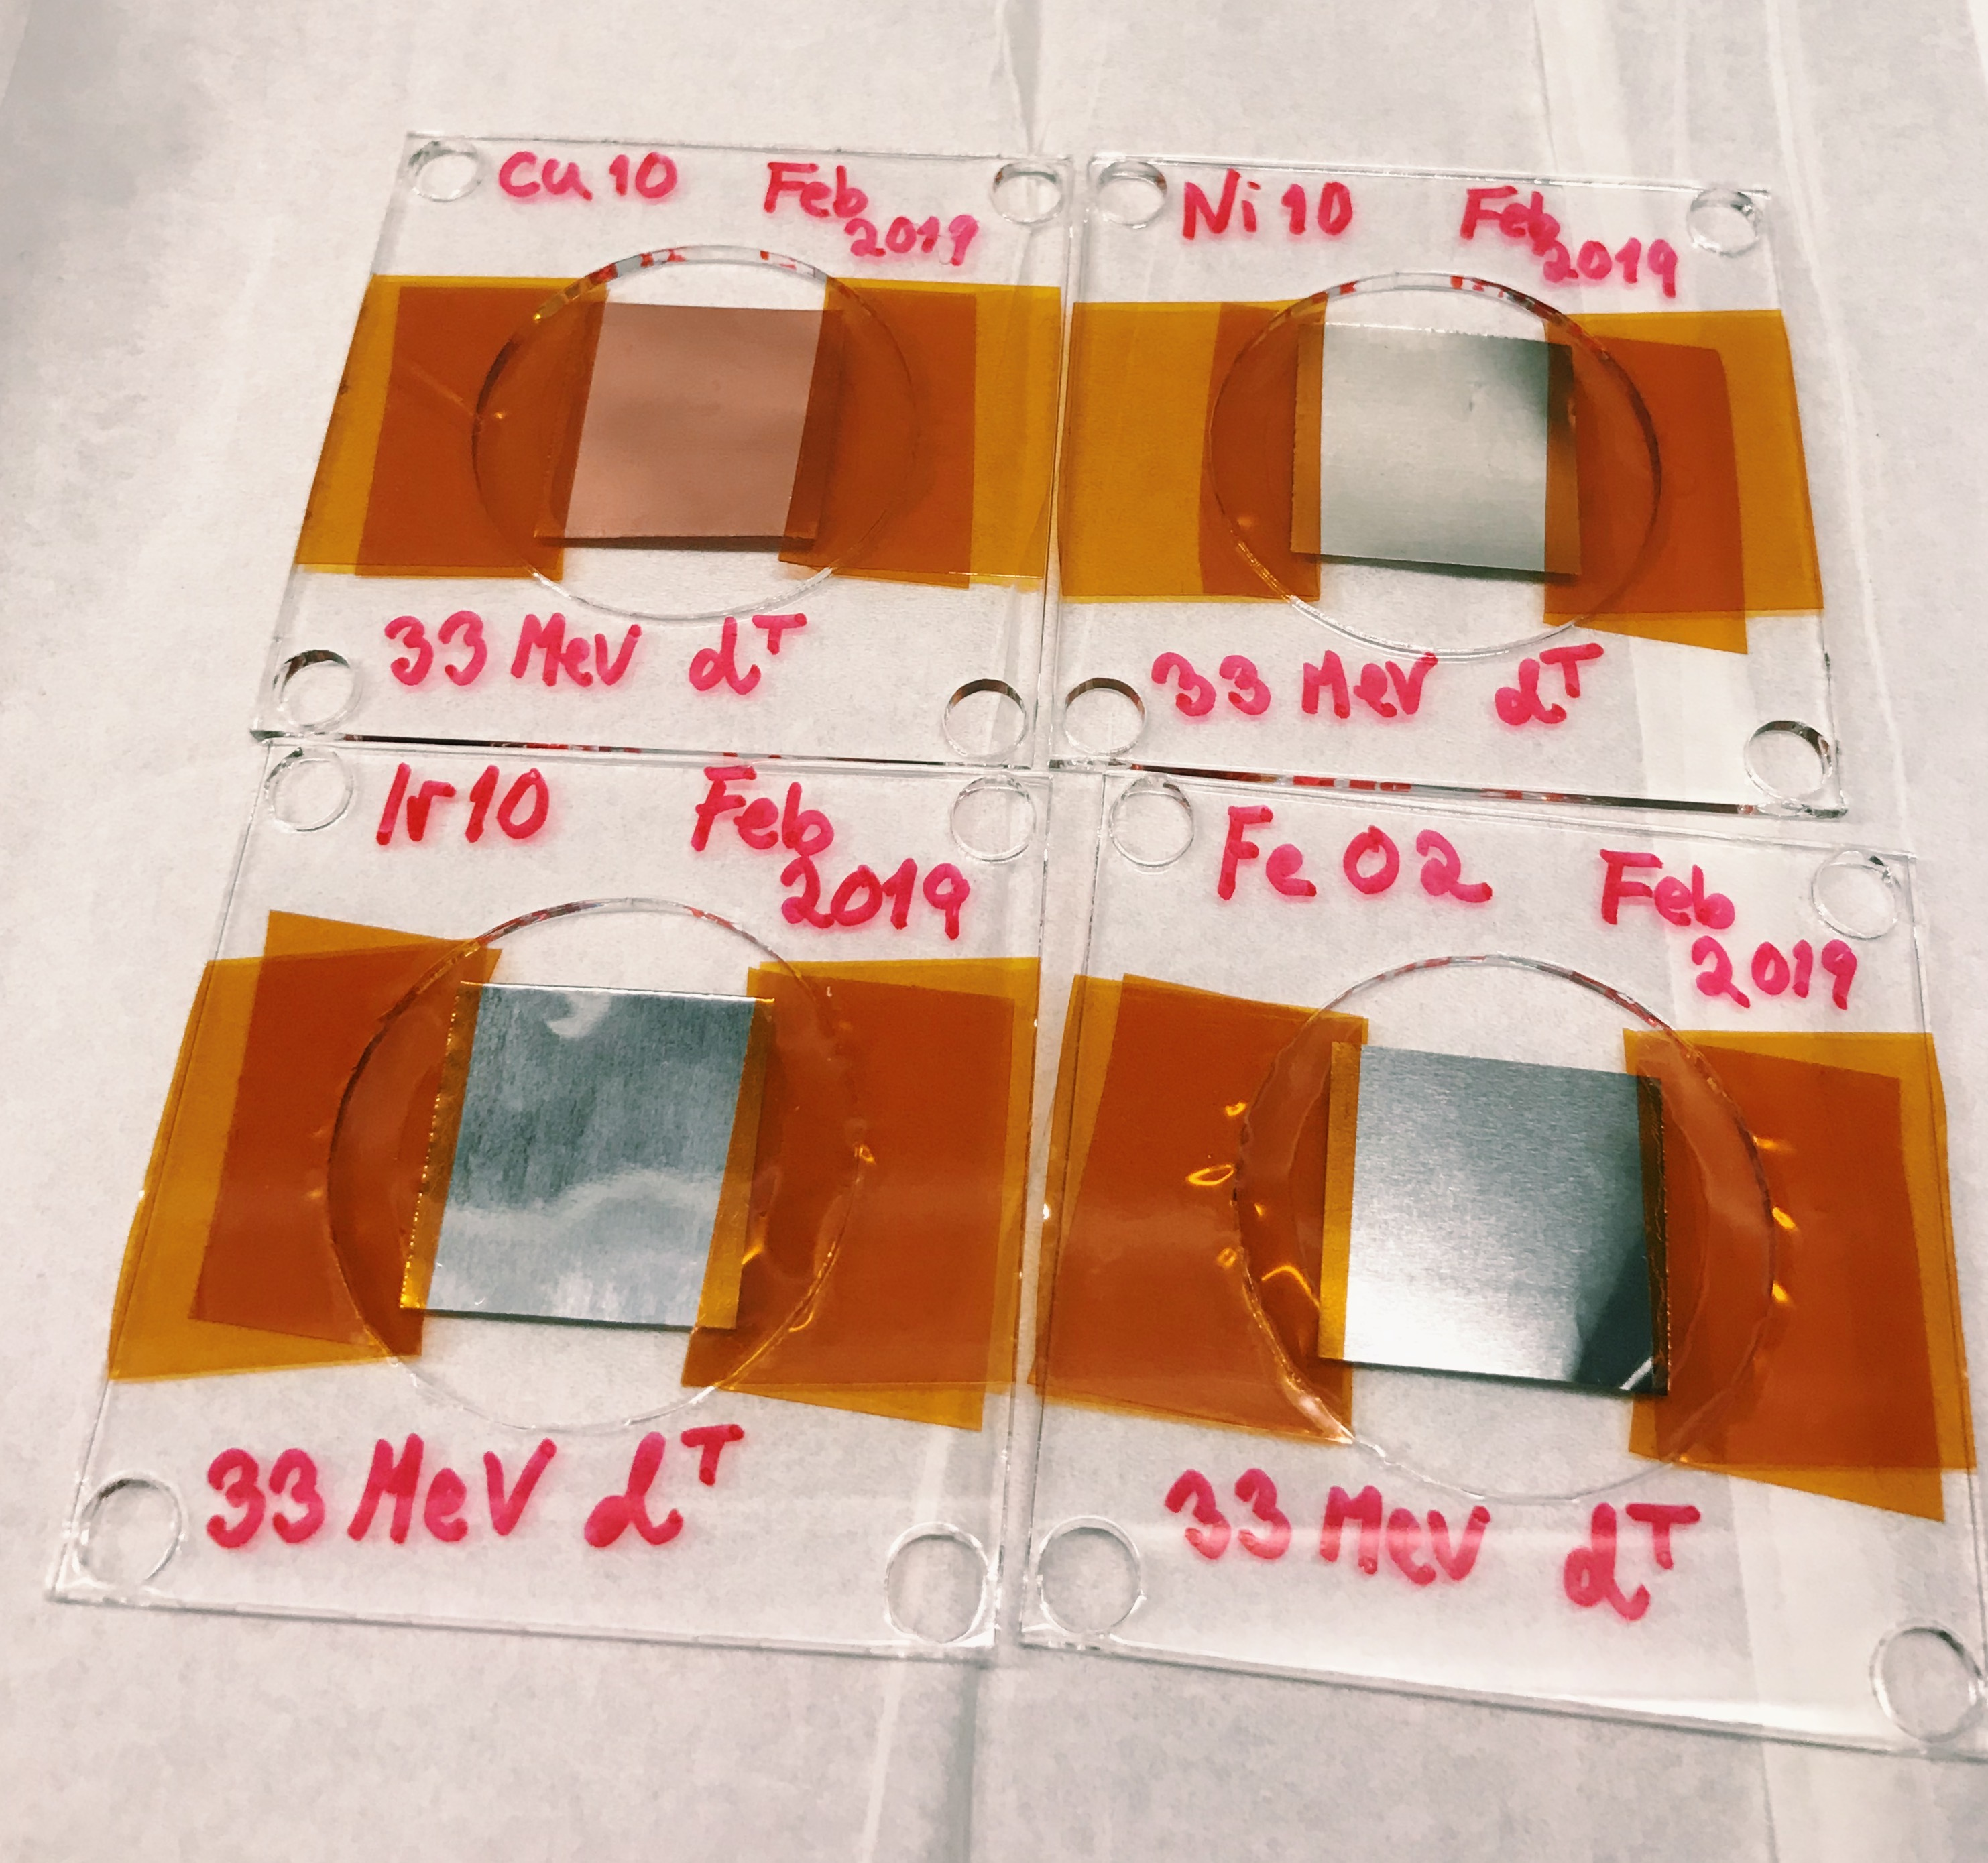
\includegraphics[width=0.5\textwidth]{Experiment/targets_on_frame.JPG}
    \caption{The figure shows the four different targets mounted on plastic frames with capton tape attached along the edges of the foils.}
    \label{fig:targets_on_frame}
\end{figure}


\begin{table}[h!]
%\centering
\caption{Characterization of each foil, along with calculated mass density. Each length is measured in mm, and mass in grams. }
\label{table:foil_characterization}
\small
\begin{tabular}{lllllll}
\makecell{\textbf{Foil}} & \makecell{Length1 (mm)}  &  \makecell{Length2 (mm)} & \makecell{Thickness (mm)} & \makecell{Mass (g)} & \makecell{\textbf{Mass density (mg/cm$^2$)}} \\ 
\hline
\makecell{SS1} & \makecell{} & \makecell{} & \makecell{} & \makecell{} & \makecell{\textbf{...}} \\
\hline
\makecell{Ni01} & \makecell{25.228} & \makecell{25.293} & \makecell{0.0285} & \makecell{0.1453} & \makecell{22.772 $\pm$ 0.138} \\
\makecell{Ir01} & \makecell{24.943} & \makecell{24.968} & \makecell{0.0295} & \makecell{0.3436} & \makecell{55.174 $\pm$ 0.053} \\
\makecell{Cu01} & \makecell{25.553} & \makecell{24.883} & \makecell{0.0341} & \makecell{0.1420} & \makecell{22.338 $\pm$ 0.048} \\
\makecell{Fe01} & \makecell{24.400} & \makecell{26.068} & \makecell{0.0278} & \makecell{0.1274} & \makecell{20.030 $\pm$ 0.110} \\
\hline
\makecell{Ni02} & \makecell{25.288} & \makecell{25.428} & \makecell{0.0295} & \makecell{0.1487} & \makecell{23.118 $\pm$ 0.096} \\
\makecell{Ir02} & \makecell{24.923} & \makecell{25.005} & \makecell{0.0278} & \makecell{0.3465} & \makecell{55.601 $\pm$ 0.238} \\
\makecell{Cu02} & \makecell{25.443} & \makecell{25.550} & \makecell{0.0348} & \makecell{0.1451} & \makecell{22.325 $\pm$ 0.028} \\
\makecell{Fe02} & \makecell{25.525} & \makecell{23.800} & \makecell{0.0274} & \makecell{0.1216} & \makecell{20.017 $\pm$ 0.034} \\
\hline
\makecell{Ni03} & \makecell{25.295} & \makecell{25.210} & \makecell{0.0270} & \makecell{0.1425} & \makecell{22.338 $\pm$ 0.066} \\
\makecell{Ir03} & \makecell{24.885} & \makecell{24.983} & \makecell{0.0243} & \makecell{0.3459} & \makecell{55.643 $\pm$ 0.121} \\
\makecell{Cu03} & \makecell{25.560} & \makecell{25.508} & \makecell{0.0343} & \makecell{0.1455} & \makecell{22.313 $\pm$ 0.043} \\
\makecell{Fe03} & \makecell{26.113} & \makecell{25.235} & \makecell{0.0310} & \makecell{0.1315} & \makecell{19.948 $\pm$ 0.114} \\
\hline
\makecell{Ni04} & \makecell{25.303} & \makecell{24.888} & \makecell{0.0273} & \makecell{0.1304} & \makecell{20.704 $\pm$ 0.068} \\
\makecell{Ir04} & \makecell{24.960} & \makecell{24.833} & \makecell{0.0261} & \makecell{0.3471} & \makecell{56.000 $\pm$ 0.109} \\
\makecell{Cu04} & \makecell{25.153} & \makecell{25.603} & \makecell{0.0333} & \makecell{0.1435} & \makecell{22.284 $\pm$ 0.027} \\
\hline
\makecell{Ni05} & \makecell{25.325} & \makecell{25.495} & \makecell{0.0263} & \makecell{0.1406} & \makecell{21.768 $\pm$ 0.045} \\
\makecell{Ir05} & \makecell{24.948} & \makecell{24.958} & \makecell{0.0256} & \makecell{0.3435} & \makecell{55.161 $\pm$ 0.081} \\
\makecell{Cu05} & \makecell{25.213} & \makecell{25.573} & \makecell{0.0334} & \makecell{0.1447} & \makecell{22.443 $\pm$ 0.028} \\
\hline
\makecell{Ni06} & \makecell{25.530} & \makecell{25.195} & \makecell{0.0285} & \makecell{0.1471} & \makecell{22.861 $\pm$ 0.123} \\
\makecell{Ir06} & \makecell{24.760} & \makecell{24.960} & 
\makecell{0.0240} & \makecell{0.3444} & \makecell{55.731 $\pm$ 0.088} \\
\makecell{Cu06} & \makecell{25.343} & \makecell{25.513} & \makecell{0.0340} & \makecell{0.1448} & \makecell{22.396 $\pm$ 0.012} \\
\hline
\makecell{Ni07} & \makecell{25.338} & \makecell{25.278} & \makecell{0.0268} & \makecell{0.1479} & \makecell{23.092 $\pm$ 0.078} \\
\makecell{Ir07} & \makecell{24.955} & \makecell{25.008} & \makecell{0.0278} & \makecell{0.3538} & \makecell{56.685 $\pm$ 0.085} \\
\makecell{Cu07} & \makecell{25.625} & \makecell{25.248} & \makecell{0.0326} & \makecell{0.1444} & \makecell{22.320 $\pm$ 0.014} \\
\hline
\makecell{Ni08} & \makecell{25.205} & \makecell{24.950} & \makecell{0.0256} & \makecell{0.1409} & \makecell{22.409 $\pm$ 0.124} \\
\makecell{Ir08} & \makecell{24.723} & \makecell{24.985} & \makecell{0.0281} & \makecell{0.3585} & \makecell{58.030 $\pm$ 0.130} \\
\makecell{Cu08} & \makecell{25.370} & \makecell{24.885} & \makecell{0.0333} & \makecell{0.1414} & \makecell{22.401 $\pm$ 0.033} \\
\hline
\makecell{Ni09} & \makecell{25.220} & \makecell{25.378} & \makecell{0.0257} & \makecell{0.1392} & \makecell{21.741 $\pm$ 0.073} \\
\makecell{Ir09} & \makecell{24.670} & \makecell{24.993} & \makecell{0.0273} & \makecell{0.3494} & \makecell{56.669 $\pm$ 0.043} \\
\makecell{Cu09} & \makecell{25.390} & \makecell{26.455} & \makecell{0.0331} & \makecell{0.1506} & \makecell{22.425 $\pm$ 0.041} \\
\hline
\makecell{Ni10} & \makecell{25.285} & \makecell{24.405} & \makecell{0.0271} & \makecell{0.1425} & \makecell{23.093 $\pm$ 0.024} \\
\makecell{Ir10} & \makecell{24.973} & \makecell{24.980} & \makecell{0.0270} & \makecell{0.3435} & \makecell{55.065 $\pm$ 0.055} \\
\makecell{Cu10} & \makecell{25.470} & \makecell{25.338} & \makecell{0.0355} & \makecell{0.1440} & \makecell{22.314 $\pm$ 0.047} \\
\hline


\hline
\makecell{SS2} & \makecell{} & \makecell{} & \makecell{} & \makecell{} & \makecell{\textbf{...}} \\
\makecell{P-degrader} & \makecell{} & \makecell{} & \makecell{} & \makecell{} & \makecell{\textbf{...}} \\
\makecell{Ni neutron monitor} & \makecell{} & \makecell{} & \makecell{} & \makecell{} & \makecell{\textbf{...}} \\
\hline
\end{tabular}
\end{table}


\subsection{Irradiation of target stack}
The irradiation included tuning of the beam and one hour of radiation over the target stack. Whenever the beam was turned on, the beam tube had to be pumped down to a vacuum, to not attenuate the beam. The target holder was a 6061 aluminum alloy with a hole in the front for the beam. The targetholder was placed in the end of the beam tube (\textcolor{red}{mounts of the end of an electrically-isolated beamline, (iron paper andrew)}). The targetholder can be visualized in figure \ref{fig:targetstack}, with a spring holding the foils stable (\ref{fig:stack}a) and placed in the end of the beam tube (\ref{fig:stack}b). 

\subsubsection{Tuning the beam}
The cyclotron was tuned for a 33 MeV deuteron beam, and needed to have the correct beam spot. First, the beam spot was visualized using a ca. 2.5 cm thick borosilicate glass, painted with a mixture of phosphor powder and vacuum grease (so that the paint does not evaporate as the tube was pumped down to vacuum). When ionizing radiation strikes the phosphor, the phosphor is excited and emits light in the de-excitation, called phosphorescence.  The glass is placed on the end of the beam tube. With a camera placed in cave 0, from the control room, the beam spot could be visualized, and could be steered to be centered and ca. 1 cm in diameter. Secondly, visualization of the beam throughout the beam stack was important to see that the beam did not diverge converge/diverge or move in the wrong direction over the target stack. Gafchromic films which change color if struck by ionizing radiation was placed in the front and the back of the target holder, separated by the spring. The films were exposed for a brief second, and the blue spot was evaluated. This was done until the beamspot was good both in the front and in the back of the stack. \\

\noindent
The beam efficiency transmission was calculated by measuring the the current at the Faraday cup right after the cyclotron vault (BS-02) and right before cave 0 (FC-01). BS-02 was measured to be 420 nA and FC-01 was measured to be 285 nA. This gave beam efficiency of transmission

$$\frac{FC-01}{BS-02}=67\% $$

\subsubsection{Irradiation of the target stack}

The targetstack was irradiated for exactly an hour, and the current was read of the beam integrator evenly, to assure that the it increased constantly. The beamcurrent from the beam integrator read 128.5 nA.  %The full scale ameperes was $2\cdot 10^{-7}$A.
Right after end of beam, the targets were sealed in plastic bags to avoid contamination. The foils were counted at the seven different detectors for the following 4 weeks after end of beam, first short counts to get as many observations as possible of the short-lived activities and longer and longer counts as the times since end of beam passes, so that the counting statistics for the longer lived activites are good. 

\begin{figure}%
    \centering
    \subfloat[The target stack in target holder]{{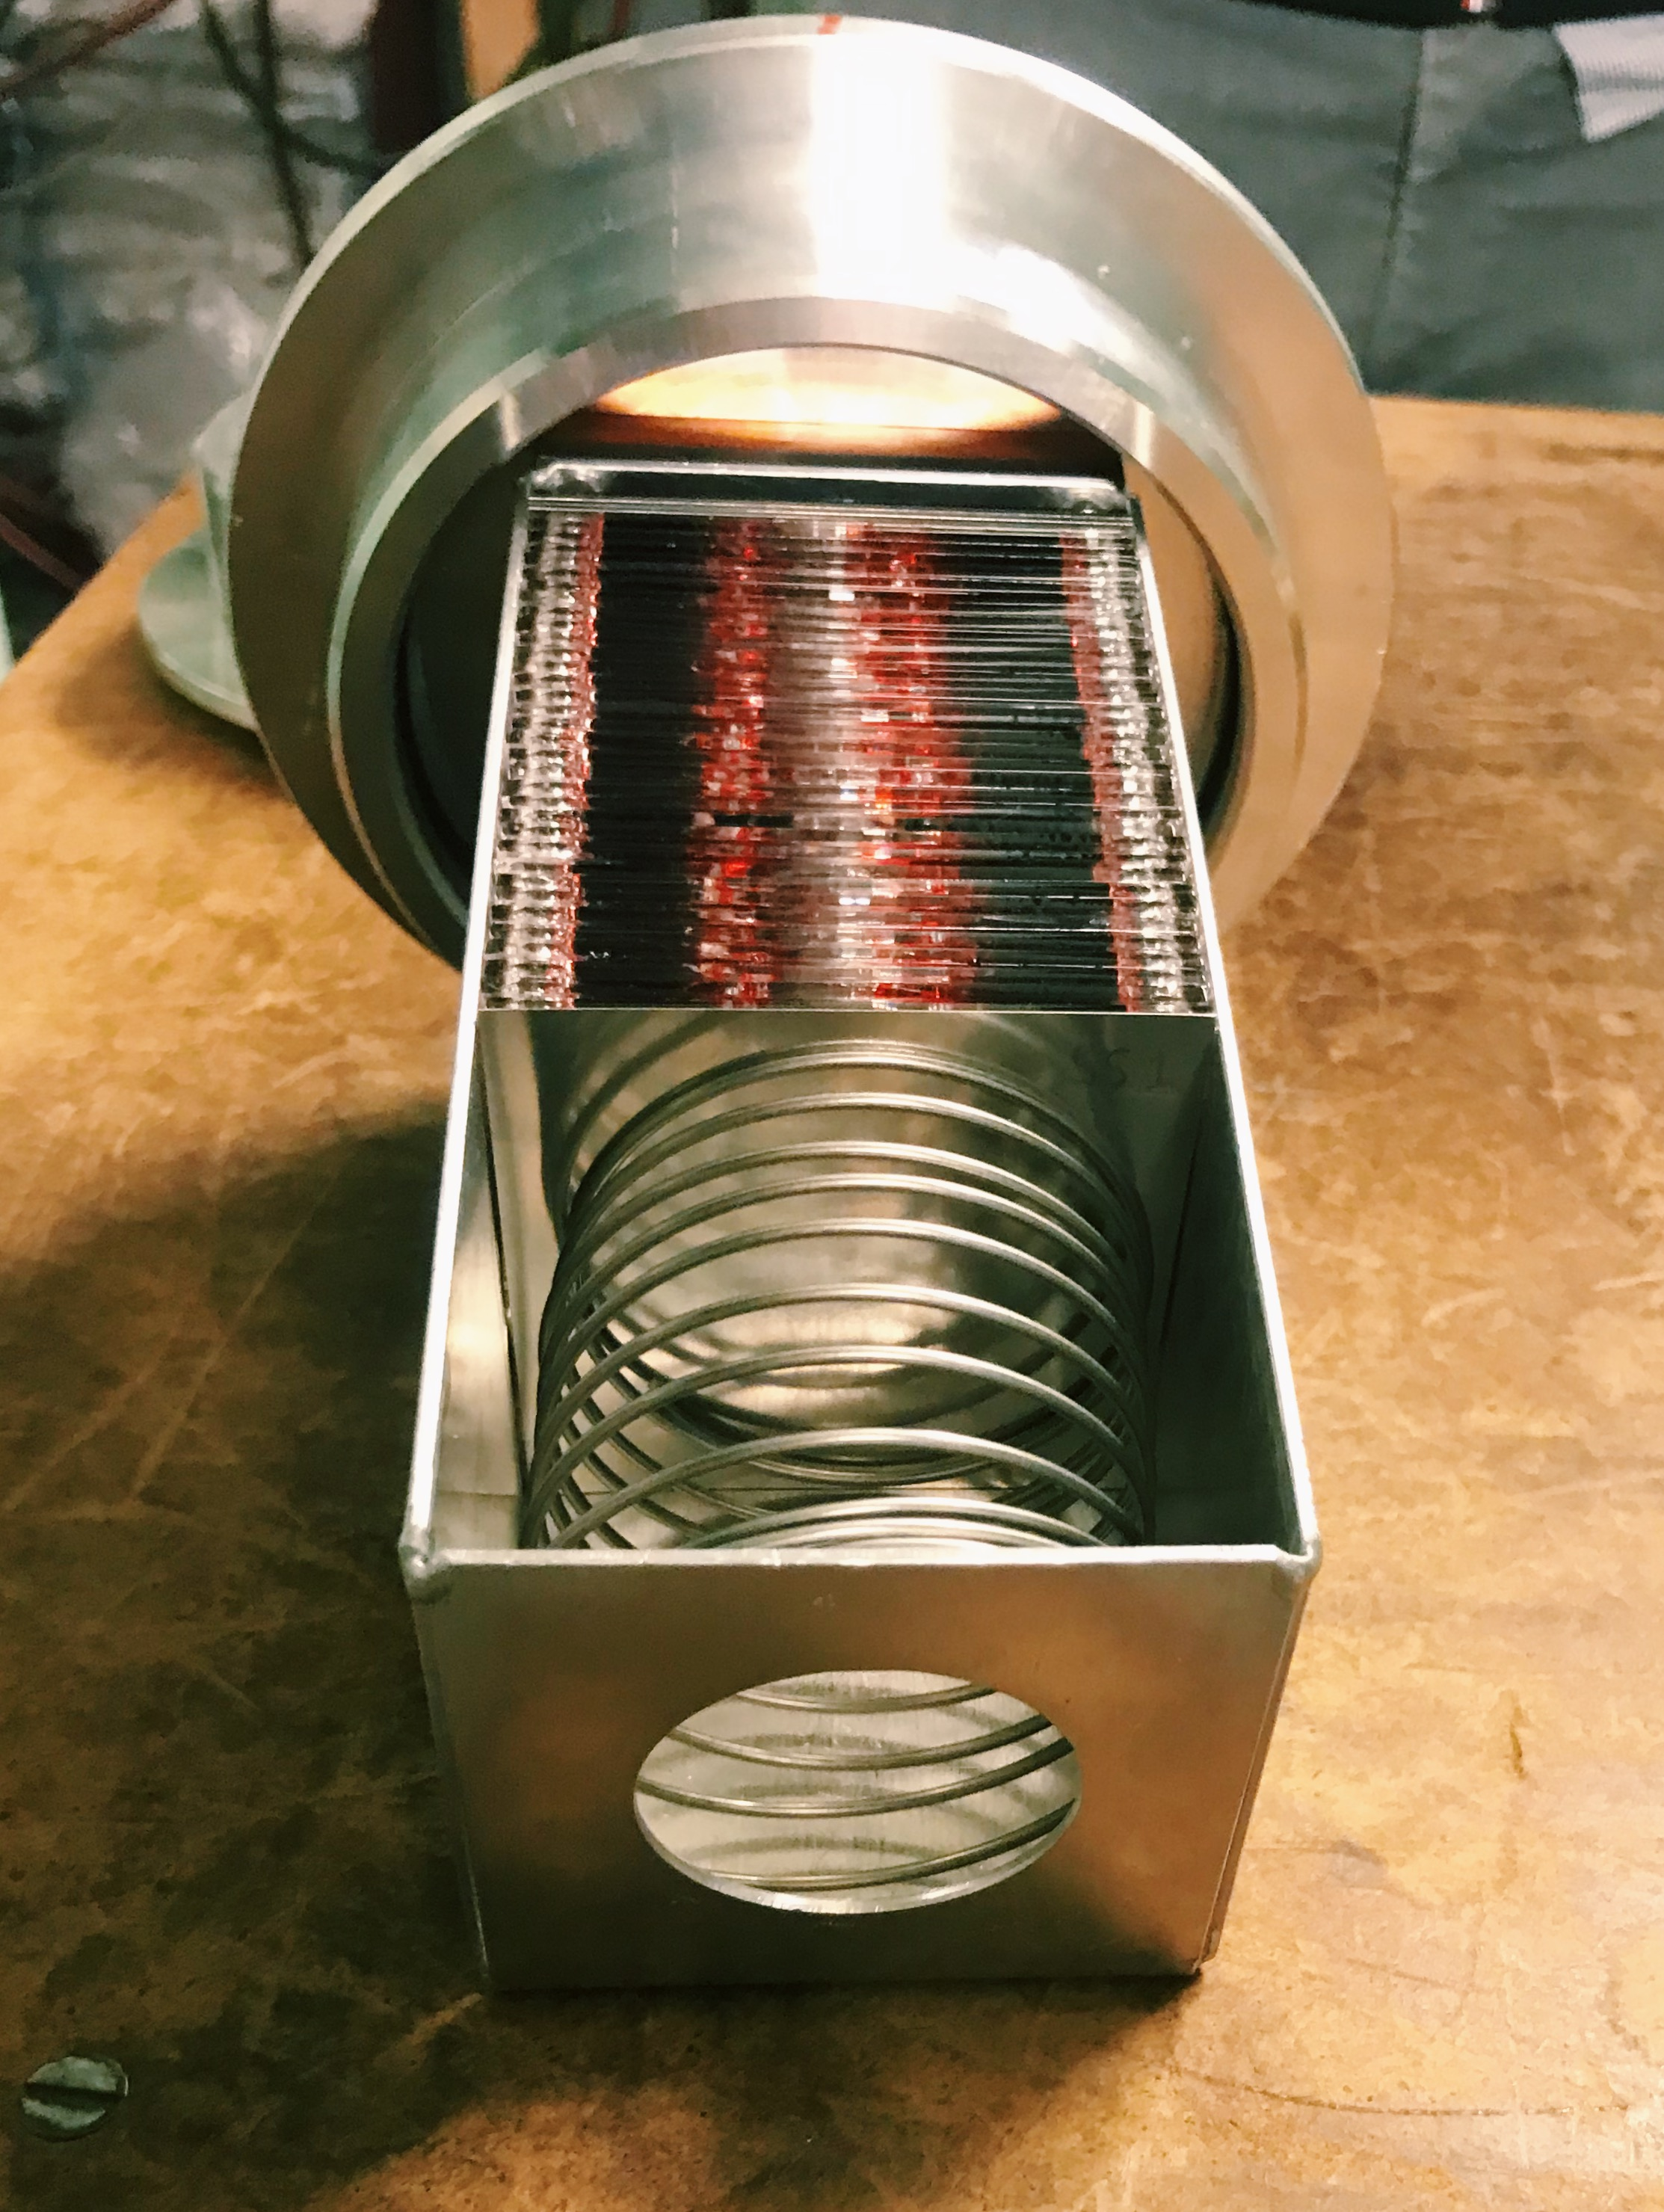
\includegraphics[width=6.6cm]{Experiment/stack.JPG} }}%
    \subfloat[Target holder placed in the end of beam tube]{{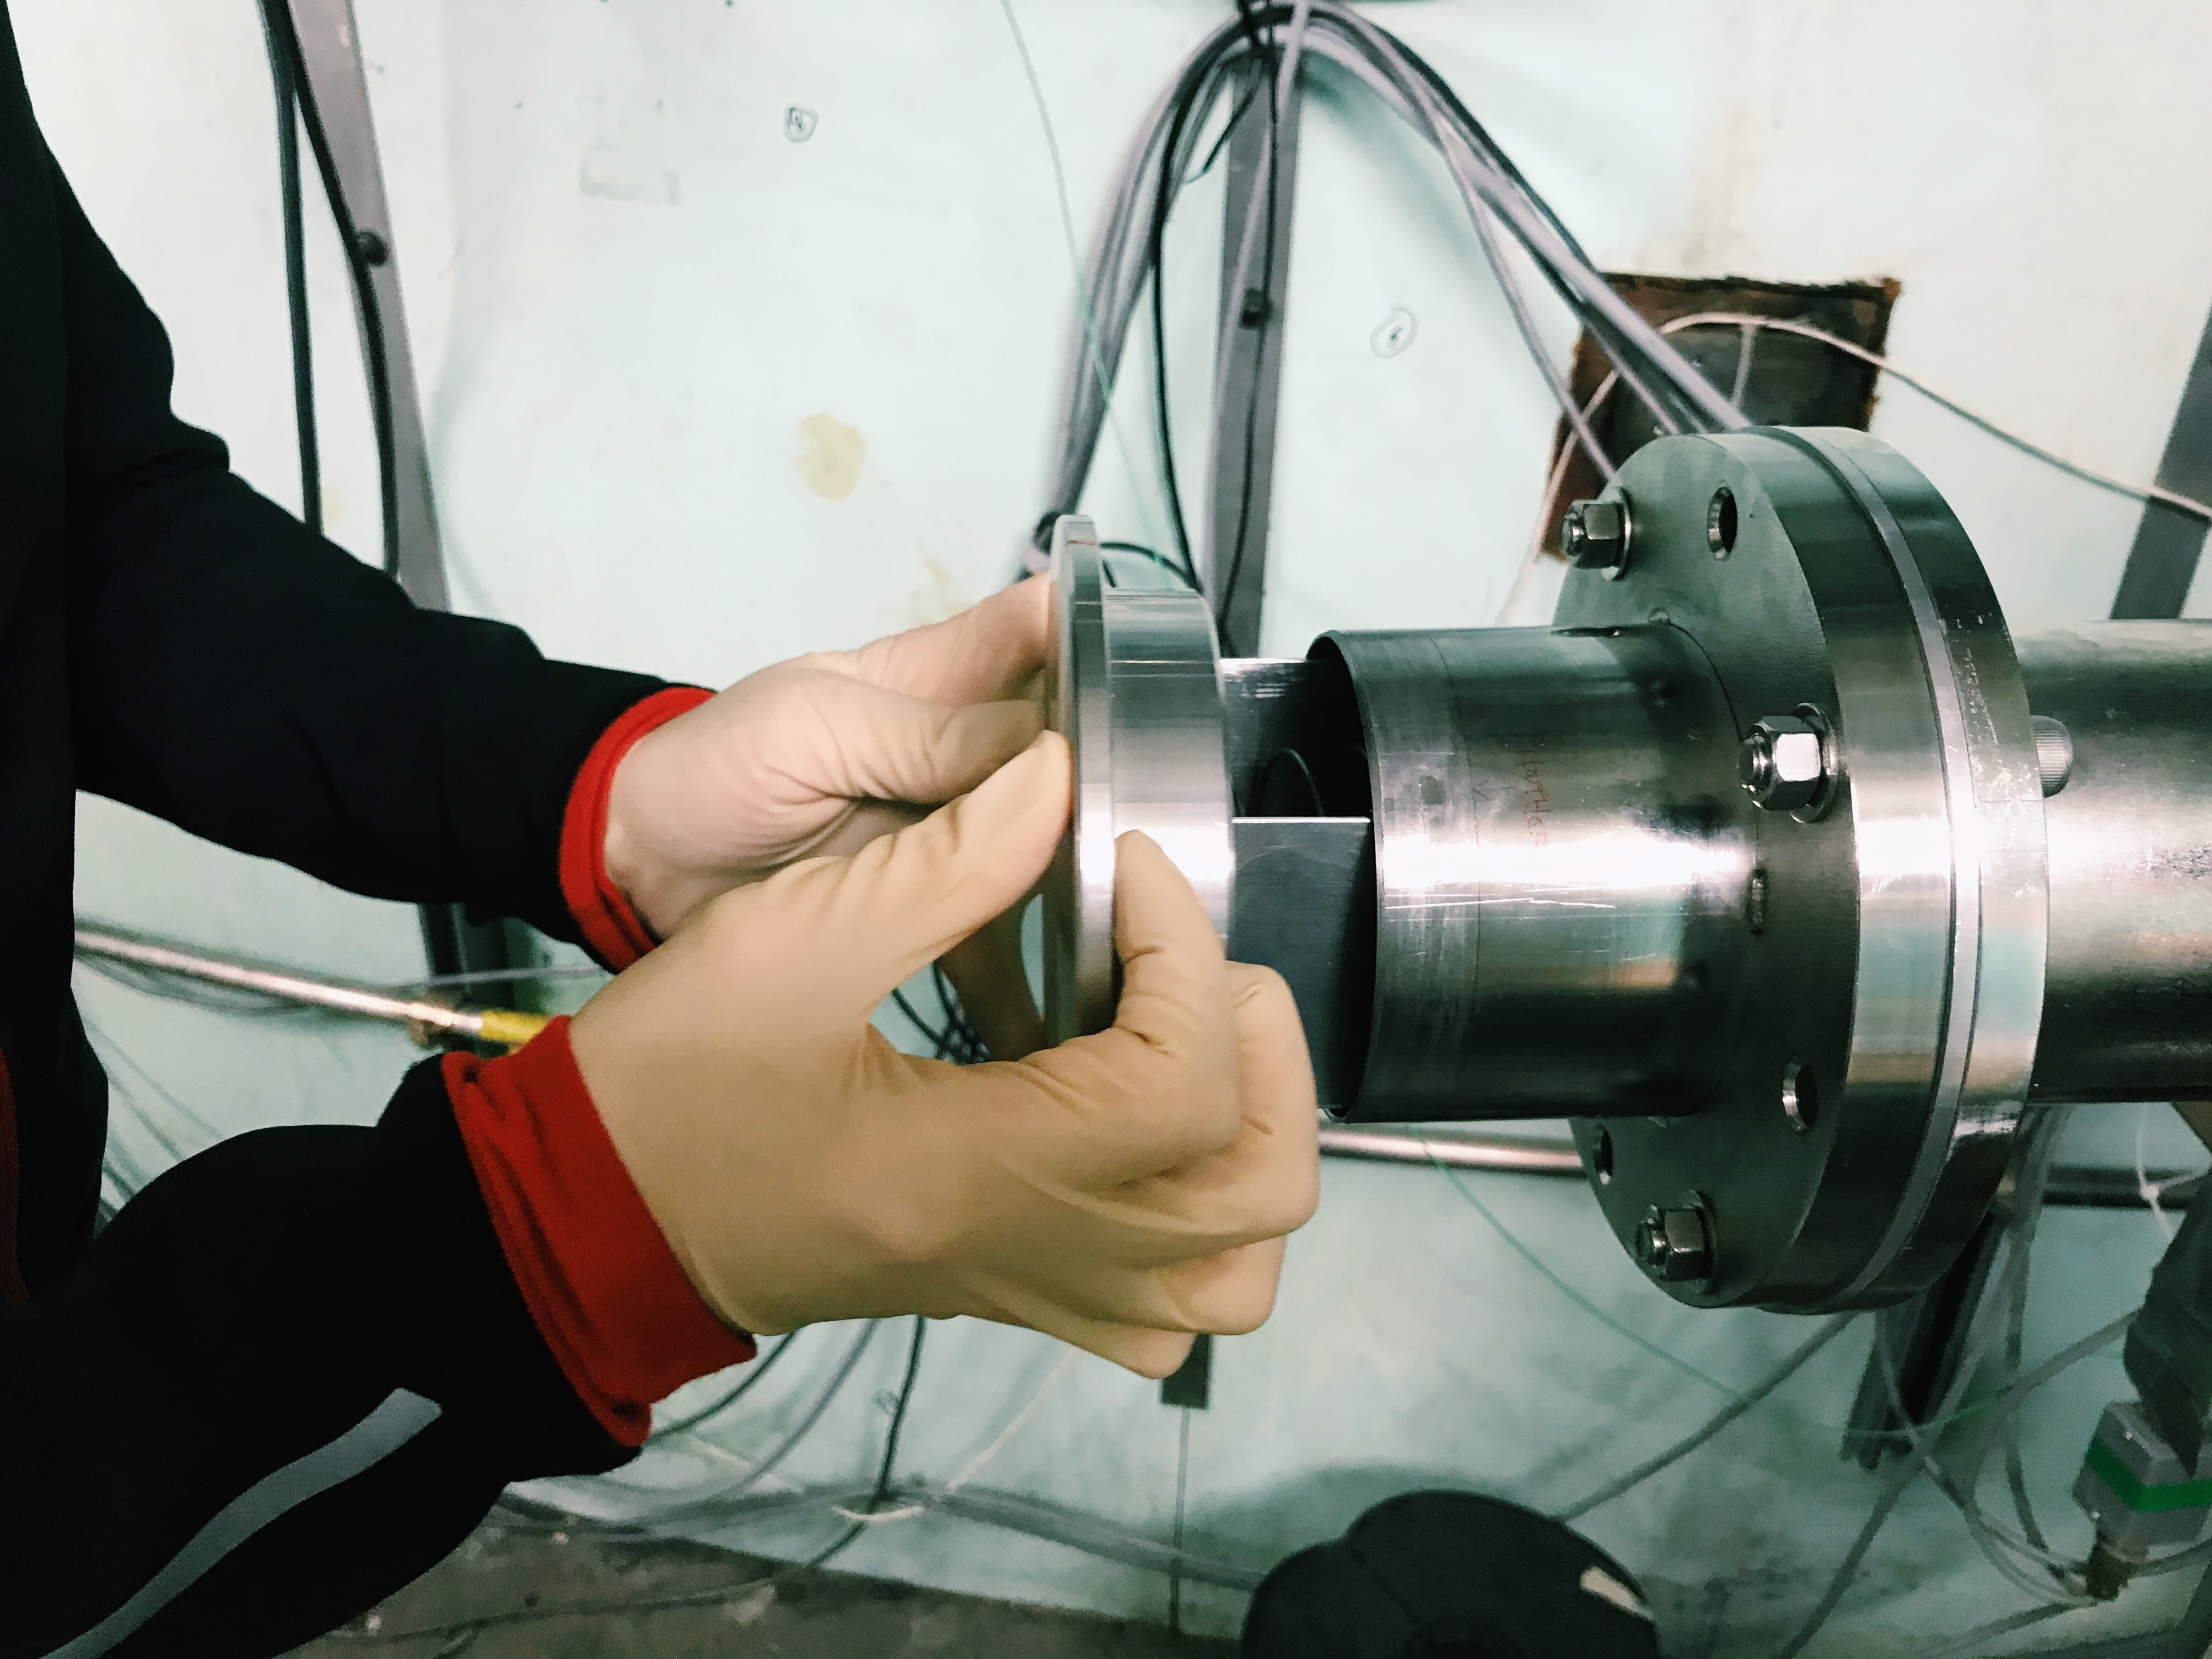
\includegraphics[width=6.6cm]{Experiment/tube.JPG} }}%
    \caption{Figure shows the target stack and how it was placed in the beam tube.}%
    \label{fig:targetstack}%
\end{figure}


\subsubsection{Intensity profile of the beam}

After irradiation, gafchromic film were attached to the activated stainless steel in the front and the back of the stack, to obtain an intensity profile of the beam. The radius of the activity from stainless on gafchromic film is used in the imaging process program Image-J, which can be seen on figure \ref{fig:SS1_gafchromic}. The gafchromic films were scanned, and the intensity data (\textcolor{red}{x and y arrays}) were obtained by inverting the scanned image, and drawing a line segment along the beam spot that automatically created an position dependent intensity array. The intensity profile can be fitted to a Gaussian, which is shown examplewise in figure \ref{fig:beamprofile}, which is the horizontal beam profile in the front and the back of the stack. In the assumption that the beam was underfilled, it was important to build confidence in that the beamspot was ca. 1 cm in diameter, which was done estimating the full width half maximum of the Gaussian profile. The FWHM over SS1 was 1.2017 cm horizontally ($\sigma^2=$0.2604 cm$^2$) and 1.1420 cm vertically ($\sigma^2=$0.2352 cm$^2$). The FWHM over SS2 was 0.6706 cm horizontally ($\sigma^2=$0.0811 cm$^2$) and 0.5783 cm vertically ($\sigma^2=$0.0603 cm$^2$). \\

\textcolor{red}{Normally the beam broadens throughout the stack due to scattering. As we can see, this not the case, since the beam is stopped in the targetstack, and therefor we do not know how much the beam truly scatters. This gives a higher uncertainty.  
The stainless steel (which consist of ..) has fast decay time. However since it emits beta-particles, the radius will slightly increase, and the true beam spot is slightly smaller. Thus the estimated FWHM values for SS1  seems to be within the criterion for underfilled targets. }



\begin{figure}
    \centering
    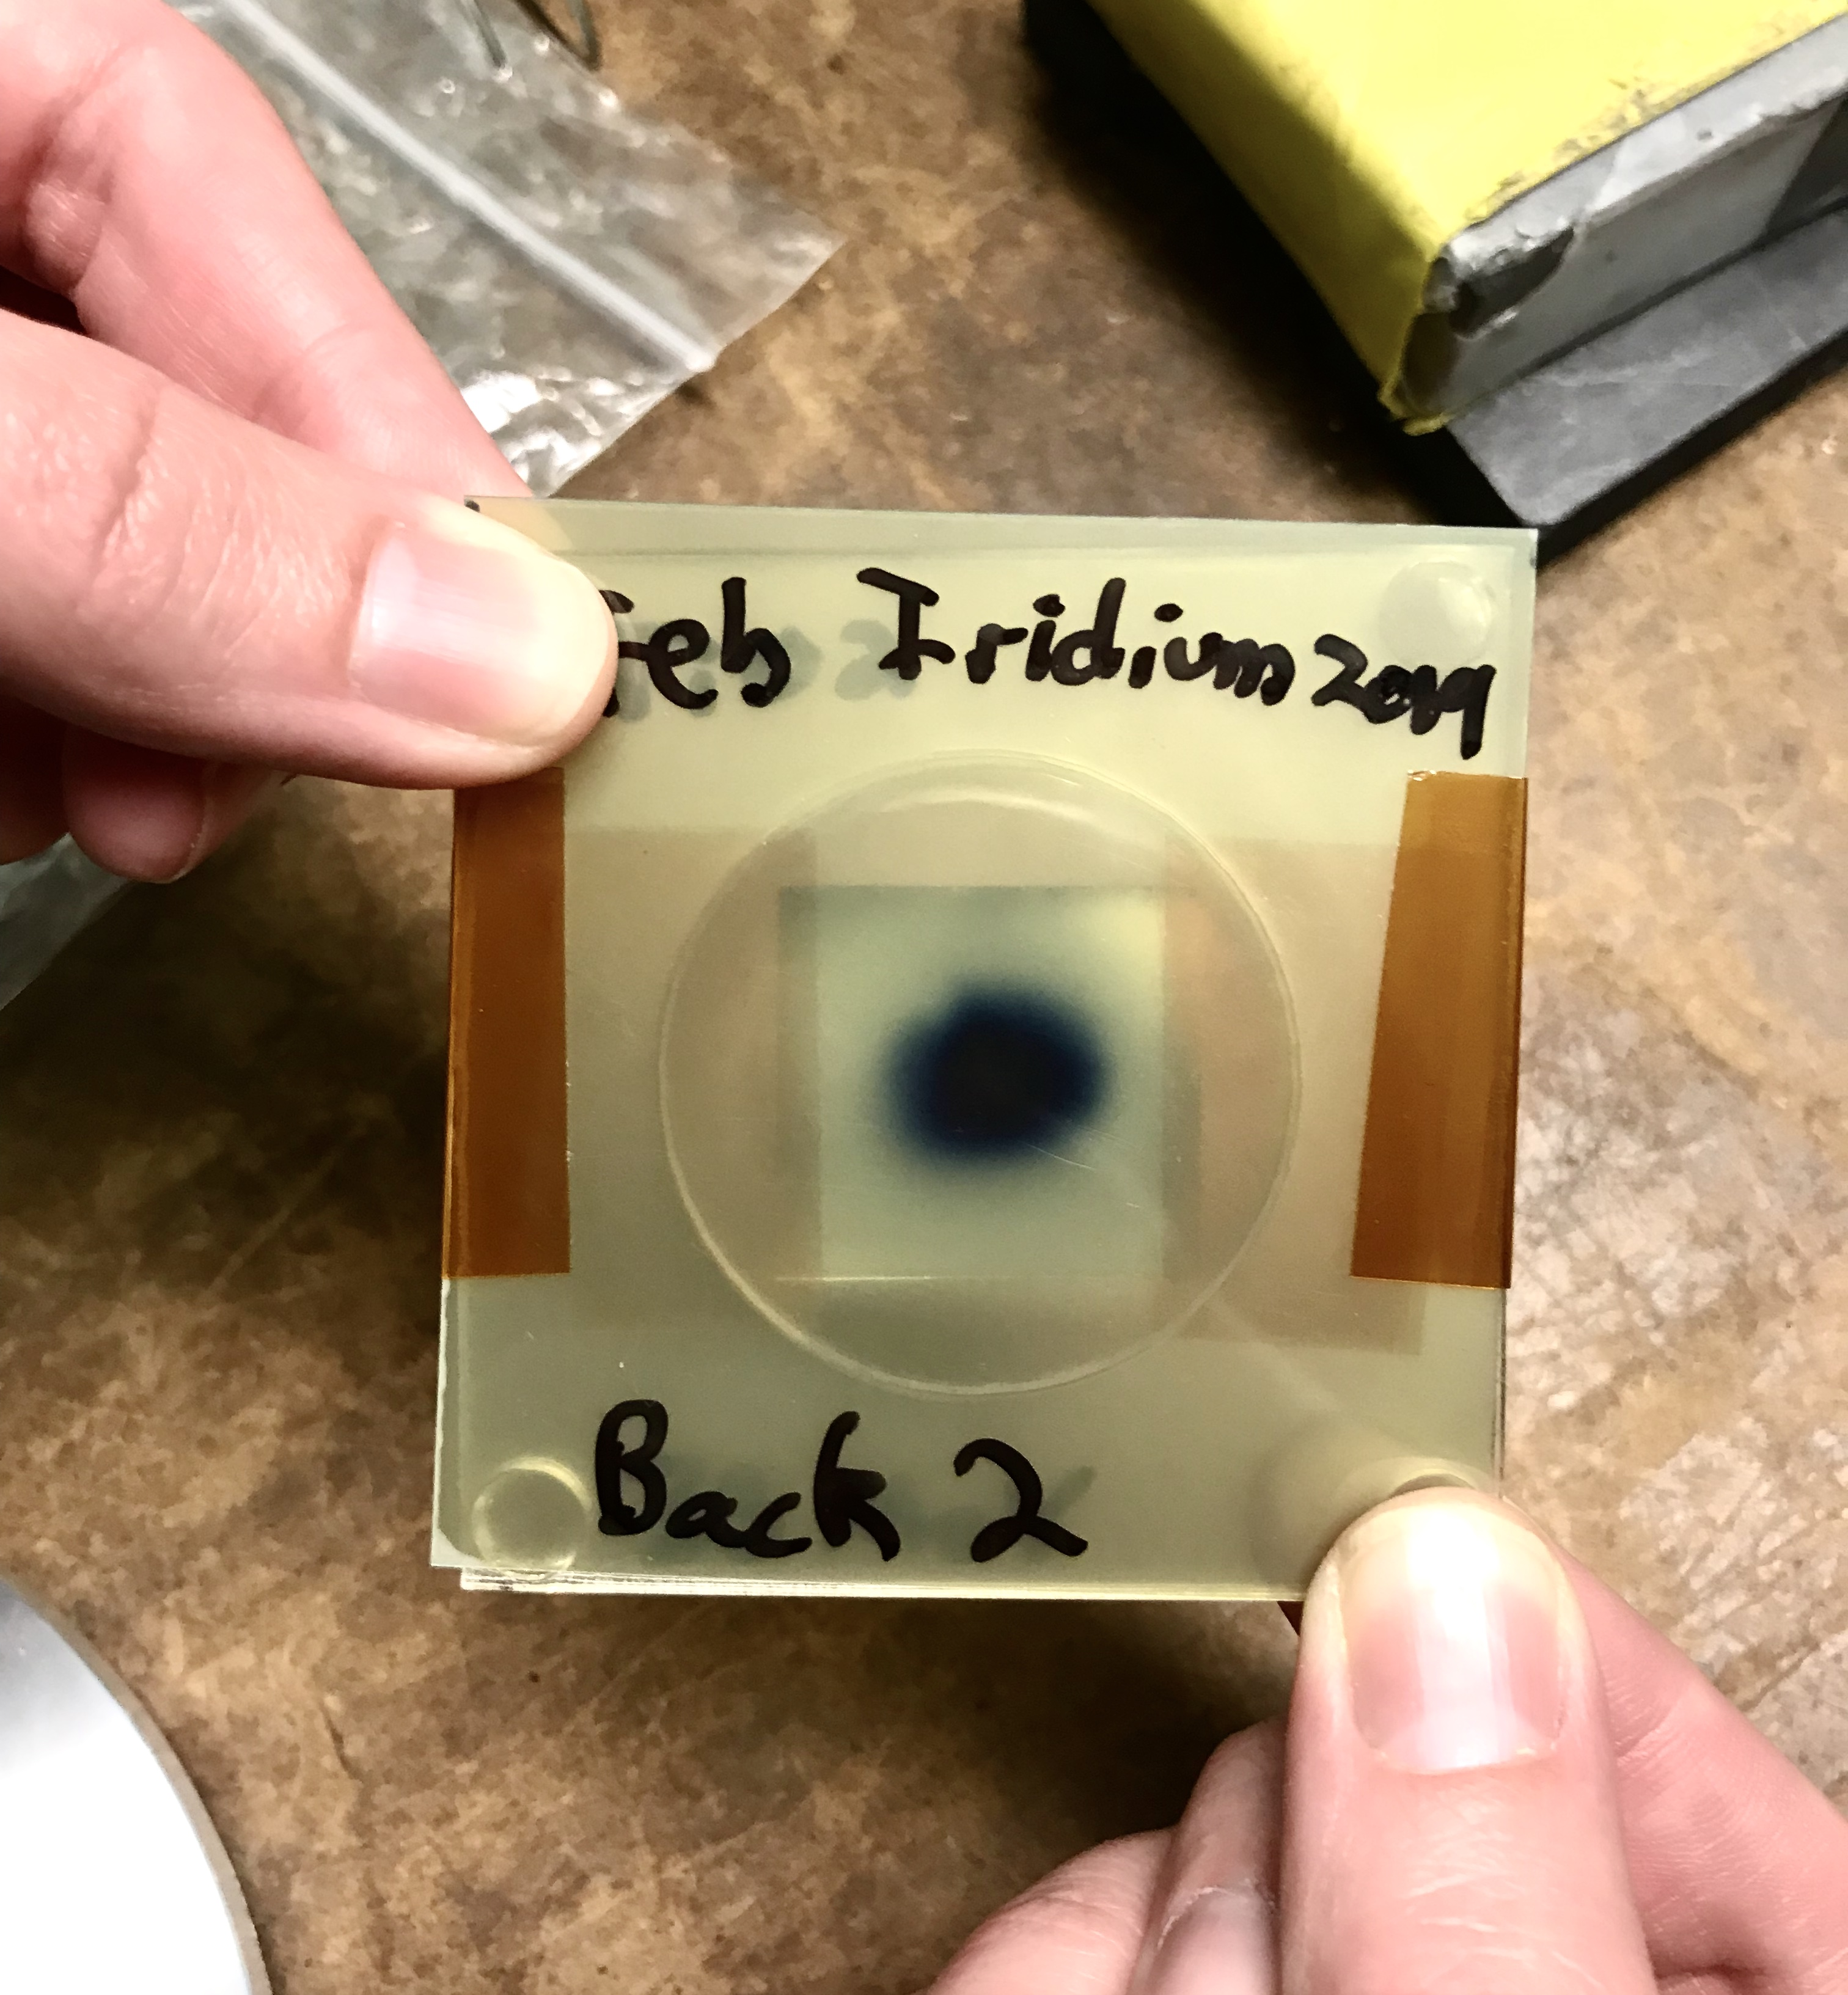
\includegraphics[width=0.3\textwidth]{Experiment/gafchromic_beamprofile.jpg}
    \caption{The gafcromic film on the activated SS1 foil. }
    \label{fig:SS1_gafchromic}
\end{figure}

\begin{figure}%
    \centering
    \subfloat[Horizontal intensity profile of SS1]{{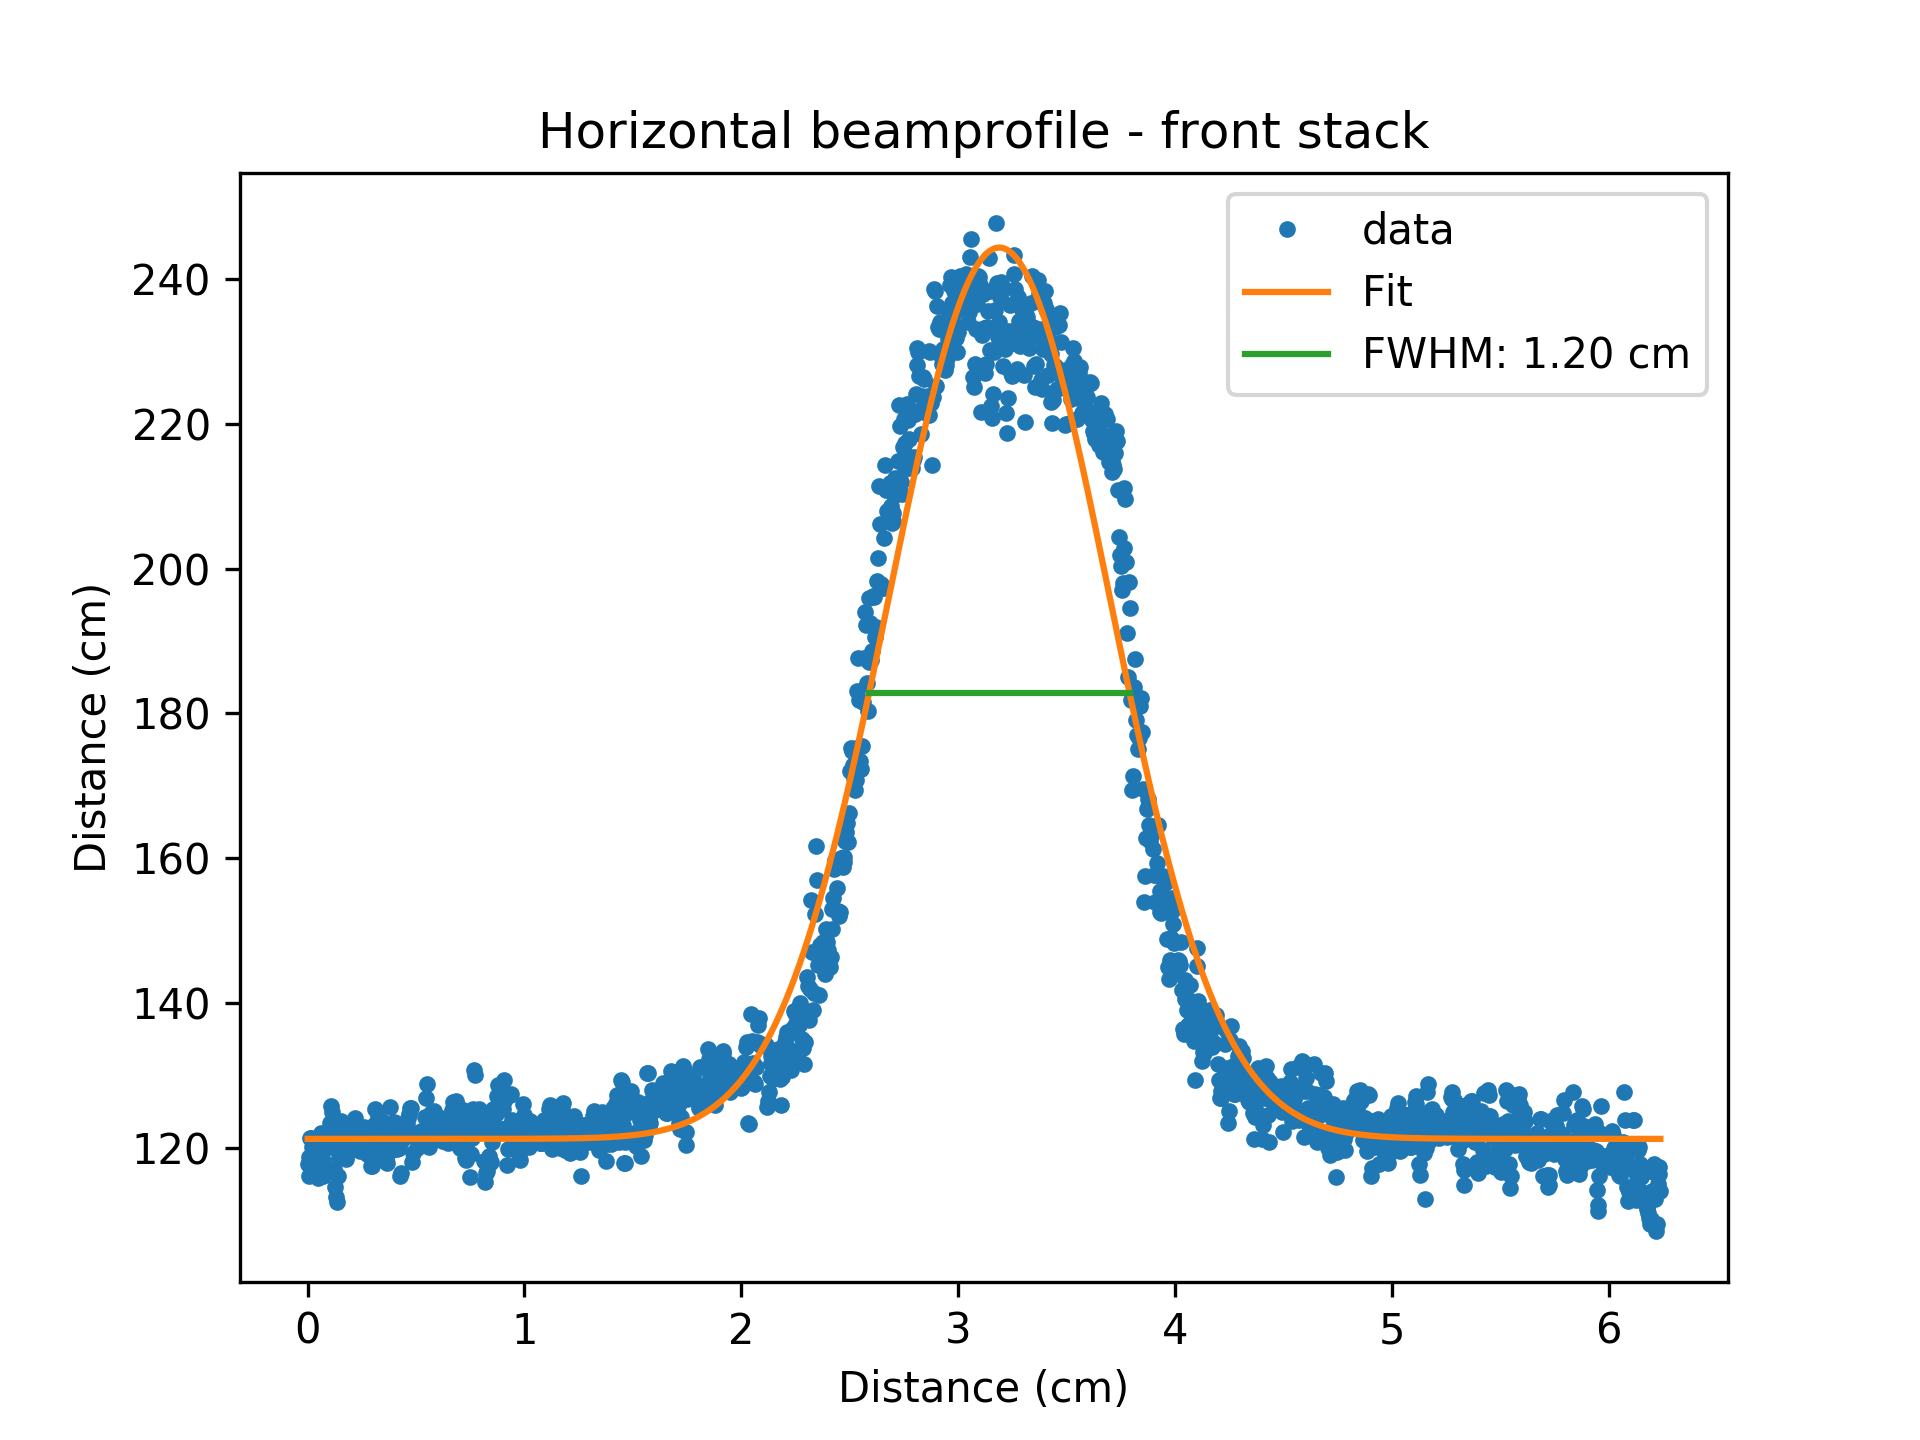
\includegraphics[width=6.6cm]{Experiment/ss_front_h.png} }}%
    
    \quad
    \subfloat[Horizontal intensity profile at SS2]{{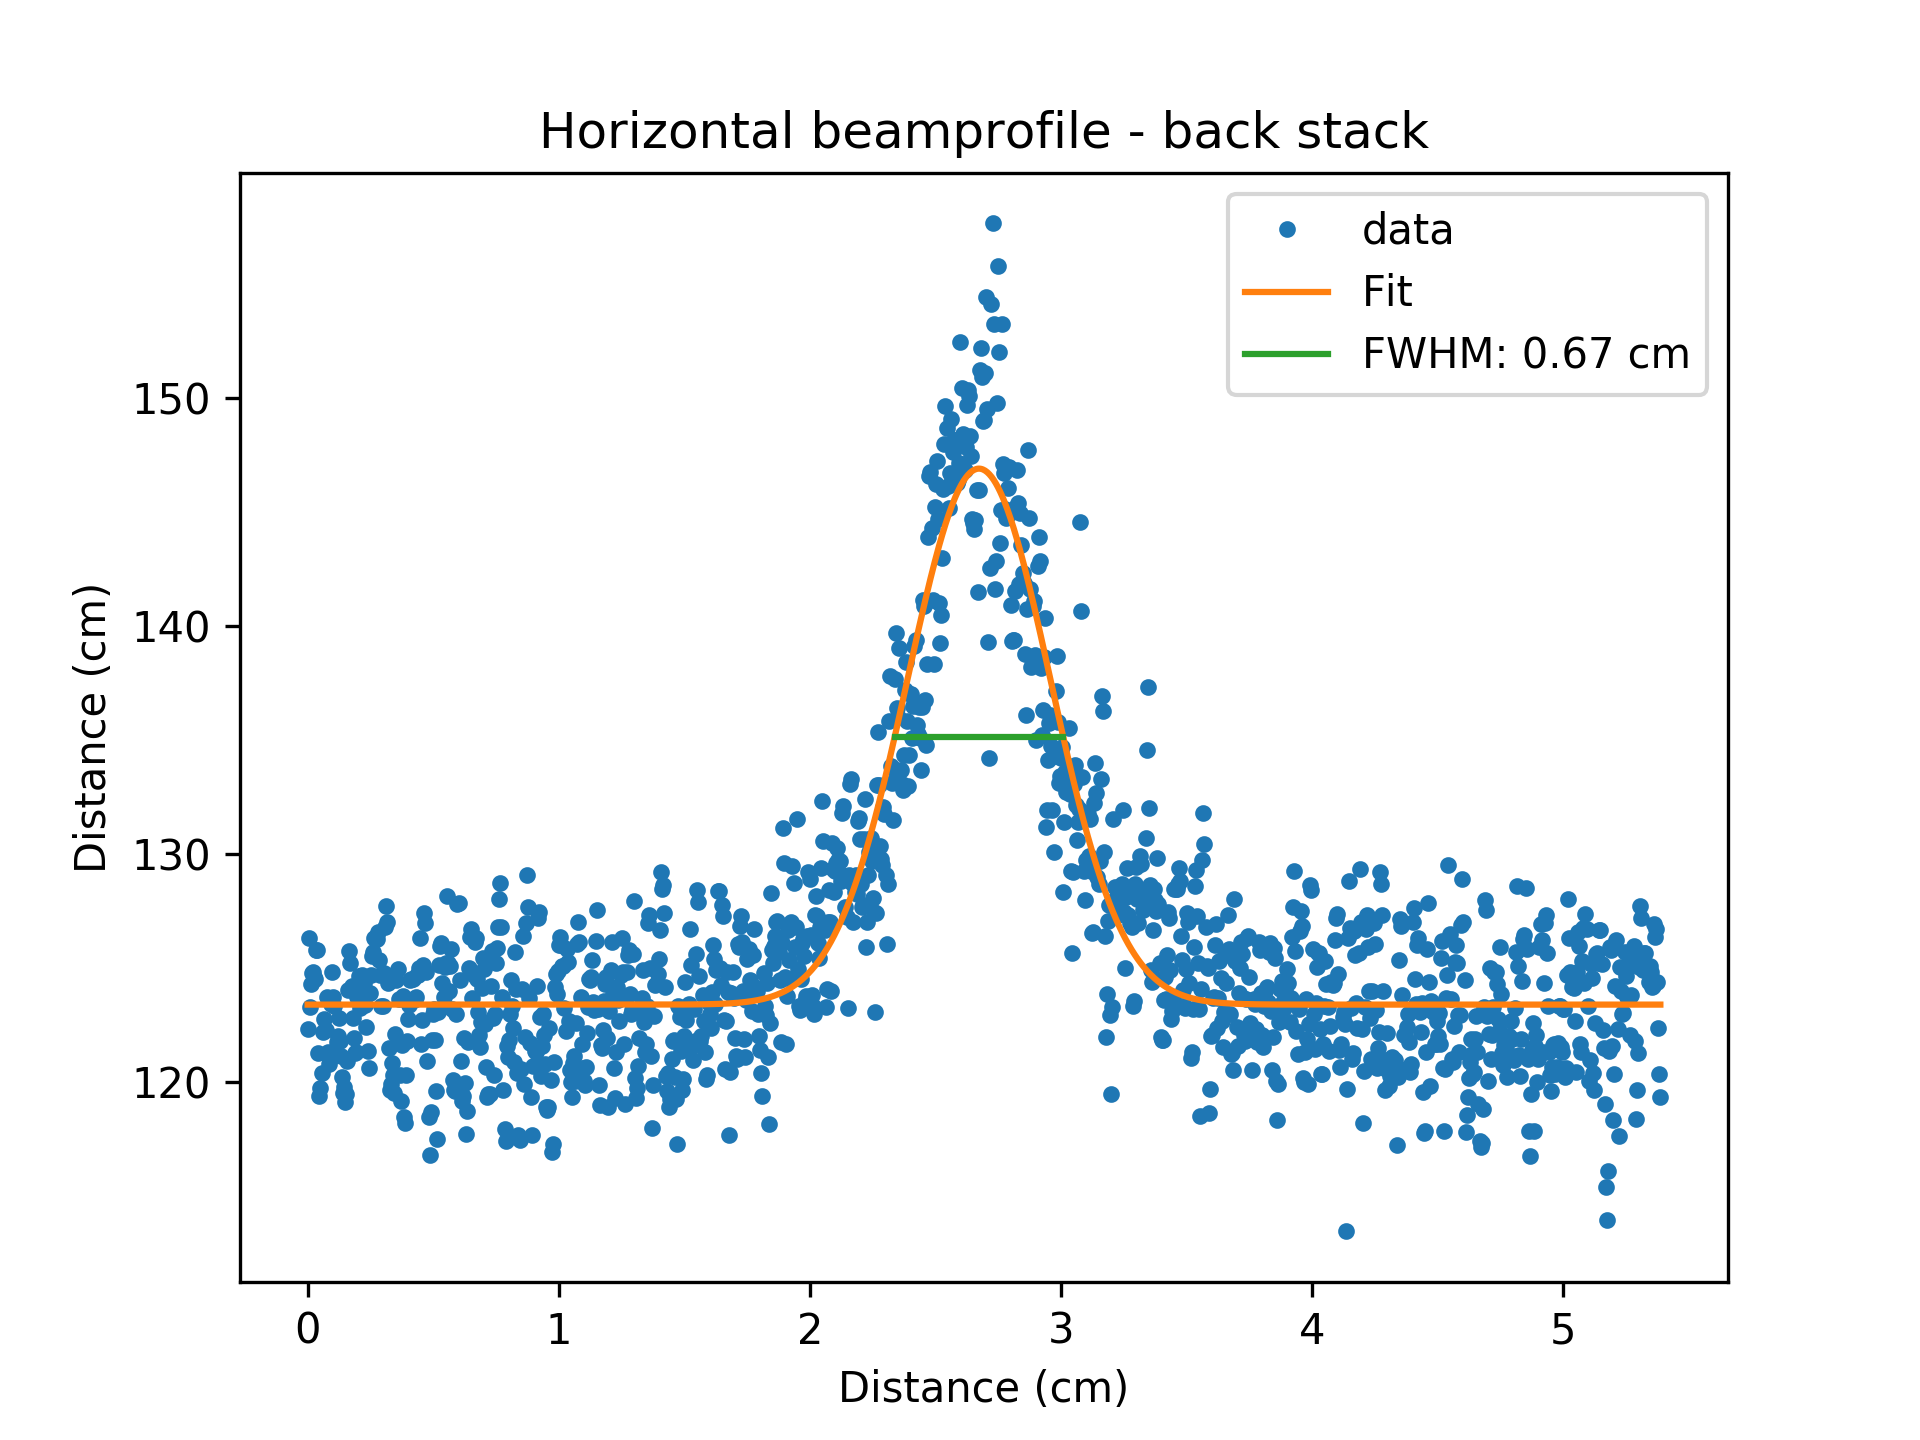
\includegraphics[width=6.6cm]{Experiment/ss_back_h.png} }}%
    \caption{Figure shows the intensity profile of the deuteron beam in the front and in the back of the stack horizontally.}%
    \label{fig:beamprofile}%
\end{figure}


\begin{figure}
    \centering
    \includegraphics[width=0.5\textwidth]{Experiment/cal_sources.png}
    \caption{The calibration point sources that were used in the efficiency calibration of the detector. ($^{22}$Na was excluded because it was difficult to work with. )}
    \label{fig:calsources}
\end{figure}

\begin{table}[]
    \centering
    \caption{The calibration point sources along with gamma lines used in the calibration of the detectors. * indicates that the value has been averaged over two peaks with similar energy, less than 1 keV. For the intensity its just added together. }
    \begin{tabular}{|cc|cc|cc|}
        \hline
        
         \multicolumn{2}{|c}{\makecell{^{137}Cs}} & \multicolumn{2}{c}{\makecell{^{133}Ba}} & \multicolumn{2}{c|}{\makecell{^{152}Eu}}\\
         %\hline 
         \Xhline{2\arrayrulewidth}
         \makecell{E_\gamma}& \makecell{I_\gamma}&\makecell{E_\gamma}& \makecell{I_\gamma}& \makecell{E_\gamma}& \makecell{I_\gamma}\\
         \hline
         \makecell{32.005^*} & \makecell{5.63^*} & \makecell{53.1622} & \makecell{2.14} & \makecell{121.7817} & \makecell{28.53}\\
         
         \makecell{36.3405^*} & \makecell{1.02^*} & \makecell{80.9979} & \makecell{32.9} & \makecell{244.6979} & \makecell{7.55}\\
         
         \makecell{661.657} & \makecell{85.10} & \makecell{160.6120} & \makecell{0.638} & \makecell{295.9387} & \makecell{0.440}\\
         
          &  & \makecell{223.2368} & \makecell{0.453} & \makecell{344.2785} & \makecell{26.5}\\
         
          &  & \makecell{276.3989} & \makecell{7.16} & \makecell{367.7891} & \makecell{0.859}\\
         
          &  & \makecell{302.8508} & \makecell{18.34} & \makecell{411.1165} & \makecell{2.237}\\
          
          
          &  & \makecell{356.0129} & \makecell{62.05} & \makecell{244.4853^*} & \makecell{3.125^*}\\
          
           &  & \makecell{383.8485} & \makecell{8.94} & \makecell{503.467} & \makecell{0.1524}\\
           
           &  & \makecell{} & \makecell{} & \makecell{586.2648} & \makecell{0.455}\\
           
           &  & \makecell{} & \makecell{} & \makecell{678.623} & \makecell{0.473}\\
           &  & \makecell{} & \makecell{} & \makecell{688.670} & \makecell{0.856}\\
           
           &  & \makecell{} & \makecell{} & \makecell{719.353^*} & \makecell{0.345^*}\\
           &  & \makecell{} & \makecell{} & \makecell{778.9045} & \makecell{12.93}\\
           &  & \makecell{} & \makecell{} & \makecell{810.451} & \makecell{0.317}\\
           &  & \makecell{} & \makecell{} & \makecell{867.380} & \makecell{4.23}\\
           &  & \makecell{} & \makecell{} & \makecell{963.712^*} & \makecell{14.65^*}\\
           &  & \makecell{} & \makecell{} & \makecell{1112.076} & \makecell{13.67}\\
           &  & \makecell{} & \makecell{} & \makecell{1212.948} & \makecell{1.415}\\
           &  & \makecell{} & \makecell{} & \makecell{1299.142} & \makecell{1.633}\\
           &  & \makecell{} & \makecell{} & \makecell{1408.013} & \makecell{20.87}\\
        %\makecell{^{137}Cs} & \makecell{^{133}Ba} & \makecell{^{152}Eu} \\
        \hline 
   
        \hline
    \end{tabular}
    \label{table:calibration_gammas}
\end{table}


\begin{comment}
\begin{table}[]
    \centering
    \caption{Table shows the geometry of the different detectors. }
    \begin{tabular}{|c|c|c|}
        \hline\textbf{}
        Detector & Geometry & Dimension \\
        \hline 
        \makecell{Detector 1} & \makecell{..} & \makecell{..} \\
        \makecell{Detector 1} & \makecell{..} & \makecell{..} \\      
        \makecell{Detector 3} & \makecell{..} & \makecell{..} \\     
        \makecell{Detector 4} & \makecell{..} & \makecell{..} \\  
        \makecell{Detector 5} & \makecell{..} & \makecell{..} \\    
        \makecell{Detector 6} & \makecell{..} & \makecell{..} \\      
        \makecell{Detector 7} & \makecell{..} & \makecell{..} \\     
        \hline
    \end{tabular}
    \label{tab:detector_characteristics}
\end{table}
\end{comment}


\subsection{Counting on high purity detectors}

\noindent 
Seven different detectors were used, six IDM Ortec detectors (detectors 1-6) with detector diameter 85 mm, detector length 30 mm and hole depth 15 mm, and one Germanium detector (detector 7) with detector diameter 64.9 mm, detector length 57.8 mm and hole depth 48.6 mm \textcolor{red}{from detector diagrams}. Besides, IDM detectors were located in cave 4c (see figure \ref{fig:LBNL_88}), which have previously been used as radiation chamber. Thus, background radiation was present. For detector 7, there was led shielding around the detector. Spectra taken on the Germanium detector is preferred. In order to visualize the signal from the detector, Maestro  (Multichannel Analyzer Emulation Software\footnote{https://www.ortec-online.com/products/application-software/maestro-mca}) was used. \\ 

\noindent 
The detectors were calibrated for efficiency, peak shape and gamma-ray energy using $^{137}$Cs ($t_{1/2}=30.08$ years\cite{Browne2007}), $^{133}$Ba ($t_{1/2}=10.551$ years\cite{Khazov2011}) and $^{152}$Eu ($t_{1/2}=13.517$ years\cite{Martin2013}) point sources, using the gammalines listed in table \ref{table:calibration_gammas}. The calibration was done at various distances from the detector surface. The point sources can can be seen on figure \ref{fig:calsources}. The energy and peakshape calibration was done in FitzPeakz which is described in section \ref{subsec:fitz_calibration}. The efficiency calibration is described in section \ref{sec:efficiency_calibration}. \\ 

\noindent 
The iridium foils were counted within 15 minutes after end of beam, and the other foils following up after. All the foils were counted for ca. four weeks following end of beam, with short counts in the beginning to have good statistical data for the short-lived activities, and longer and longer counts as the shorter and medium-lived activities decayed out, to have good statistics (enough counts). Since the detectors were calibrated at various distances, the deadtime of the foils right after end of beam could be reduced, however, as high as  16-22\% deadtime was present, but reduced to less than 5\% within a certain time after end of beam. 



\begin{comment}
\begin{figure}%
    \centering
    \subfloat[]{{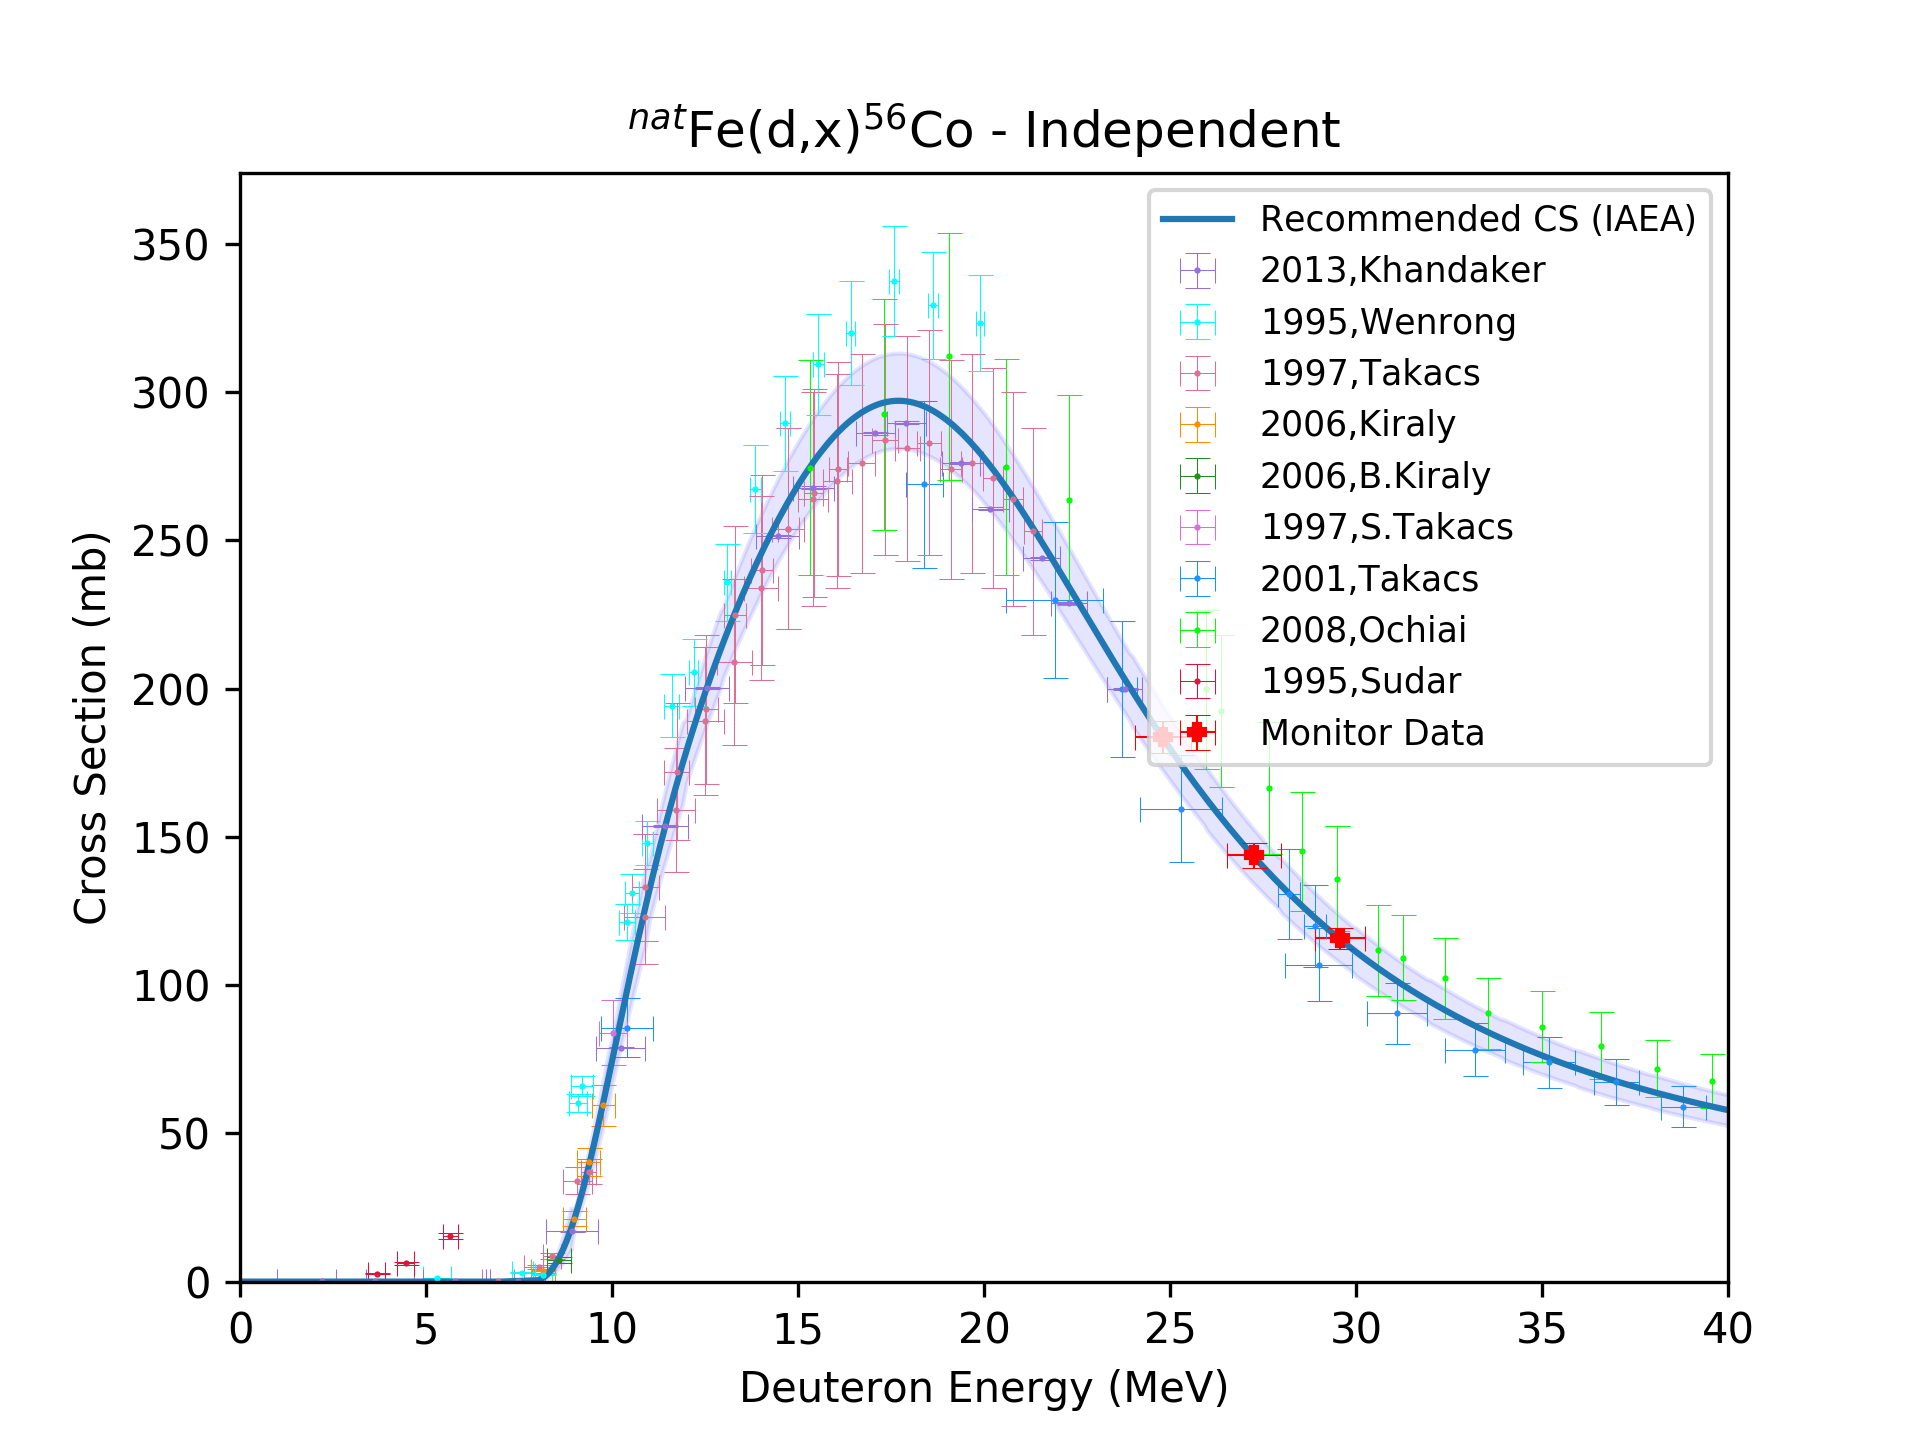
\includegraphics[width=5cm]{Fe_56Co.png} }}%
    \quad
    \subfloat[]{{\includegraphics[width=5cm]{Ni_61Cu.png} }}%
    \subfloat[]{{\includegraphics[width=5cm]{Ni_56Co.png} }}%
    \quad
    \subfloat[]{{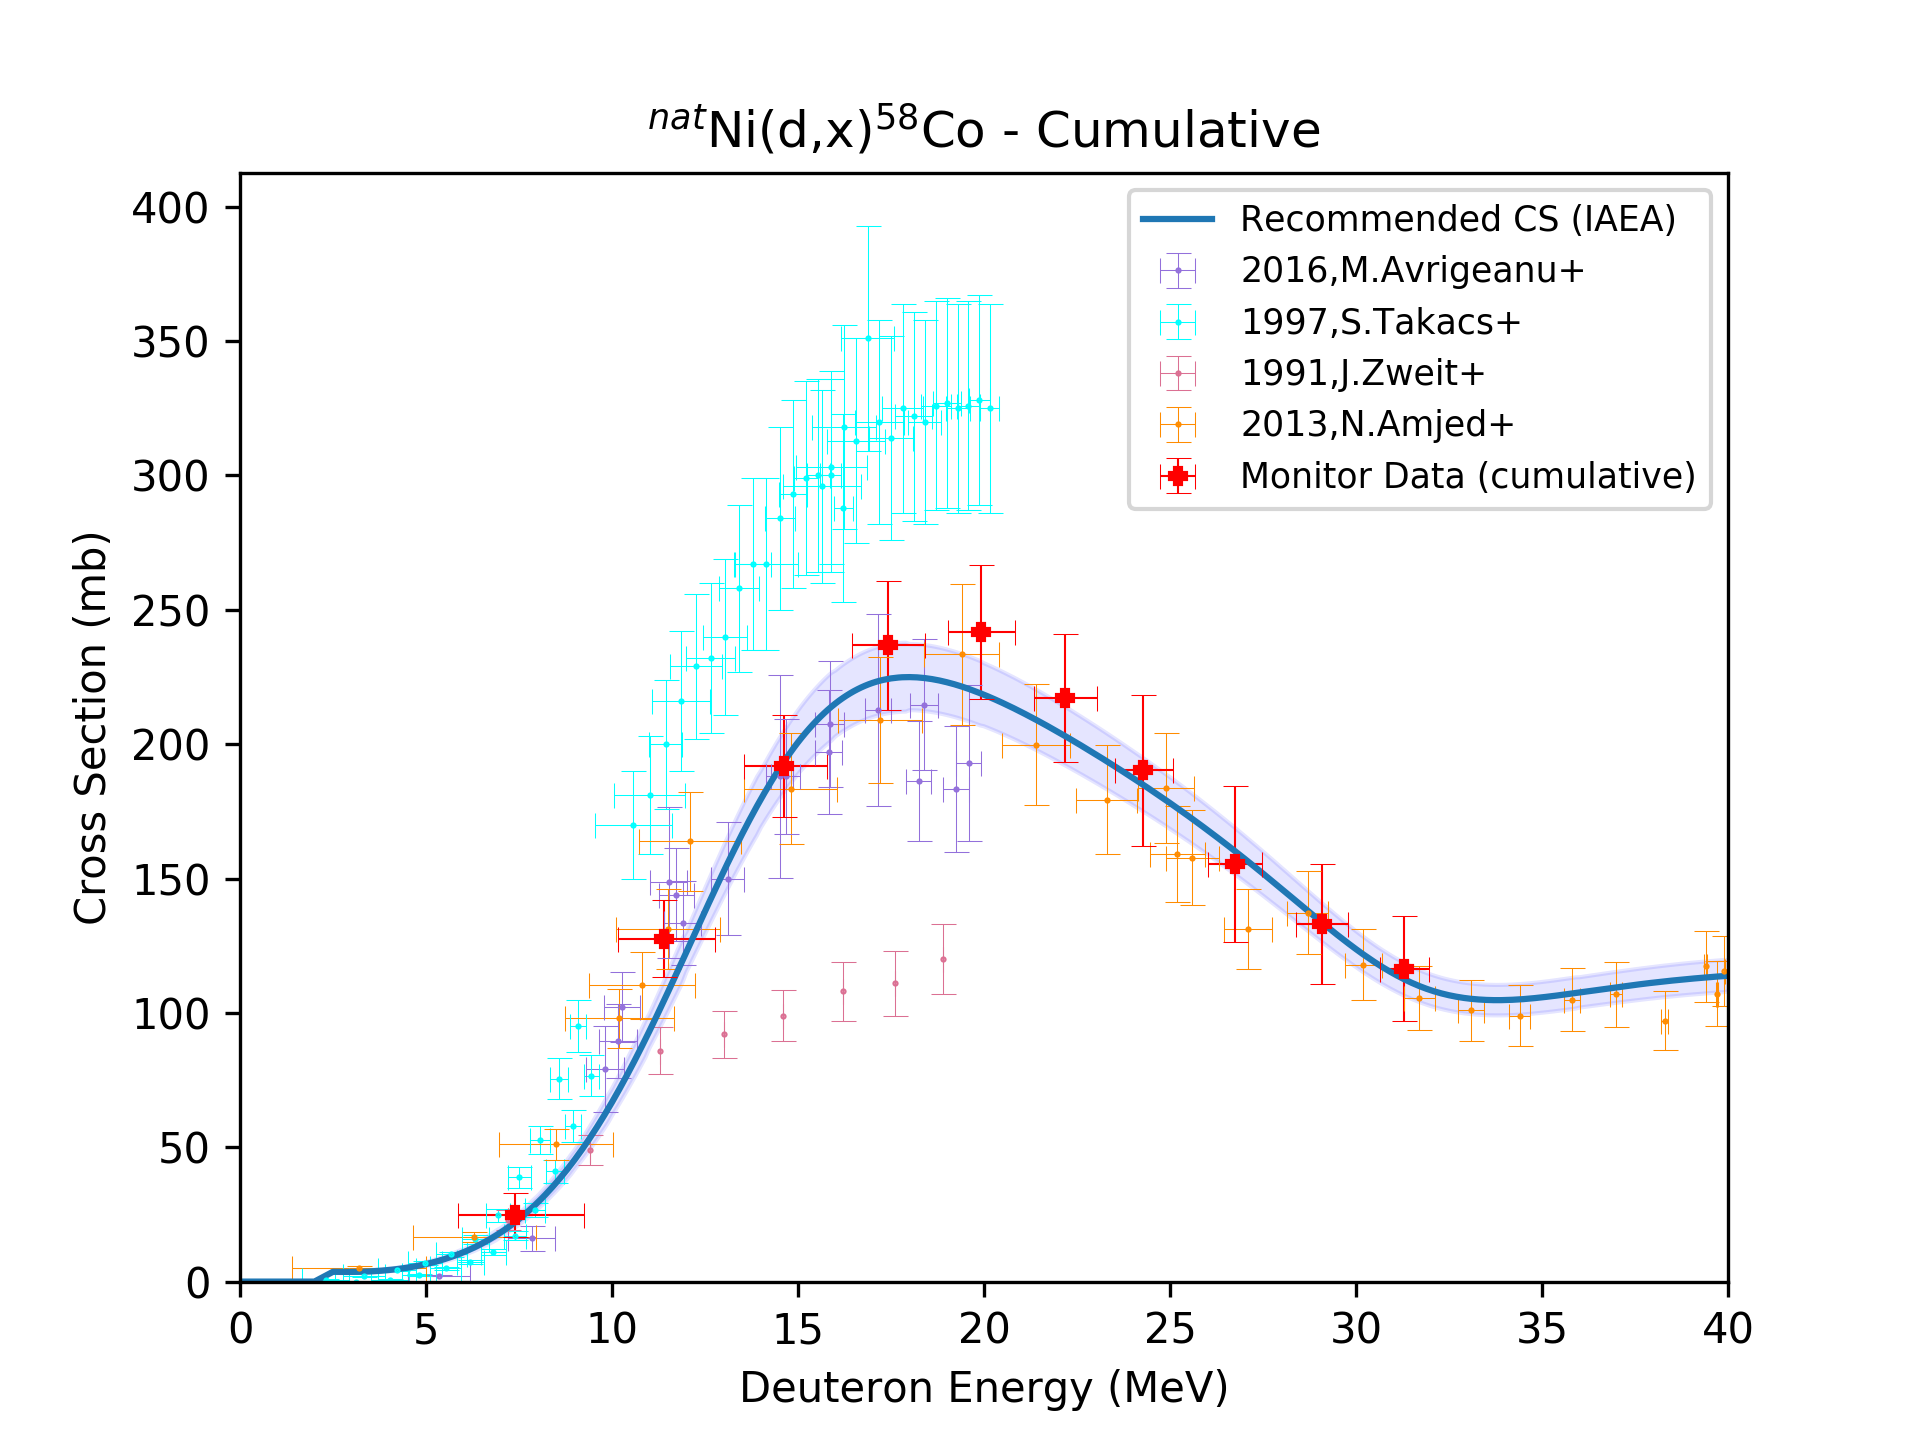
\includegraphics[width=5cm]{Ni_58Co.png} }}%
    \quad
    \subfloat[caption]{{\includegraphics[width=5cm]{Cu_62Zn.png} }}%
    \quad
    \subfloat[]{{\includegraphics[width=5cm]{Cu_63Zn.png} }}%
    \quad
    \subfloat[]{{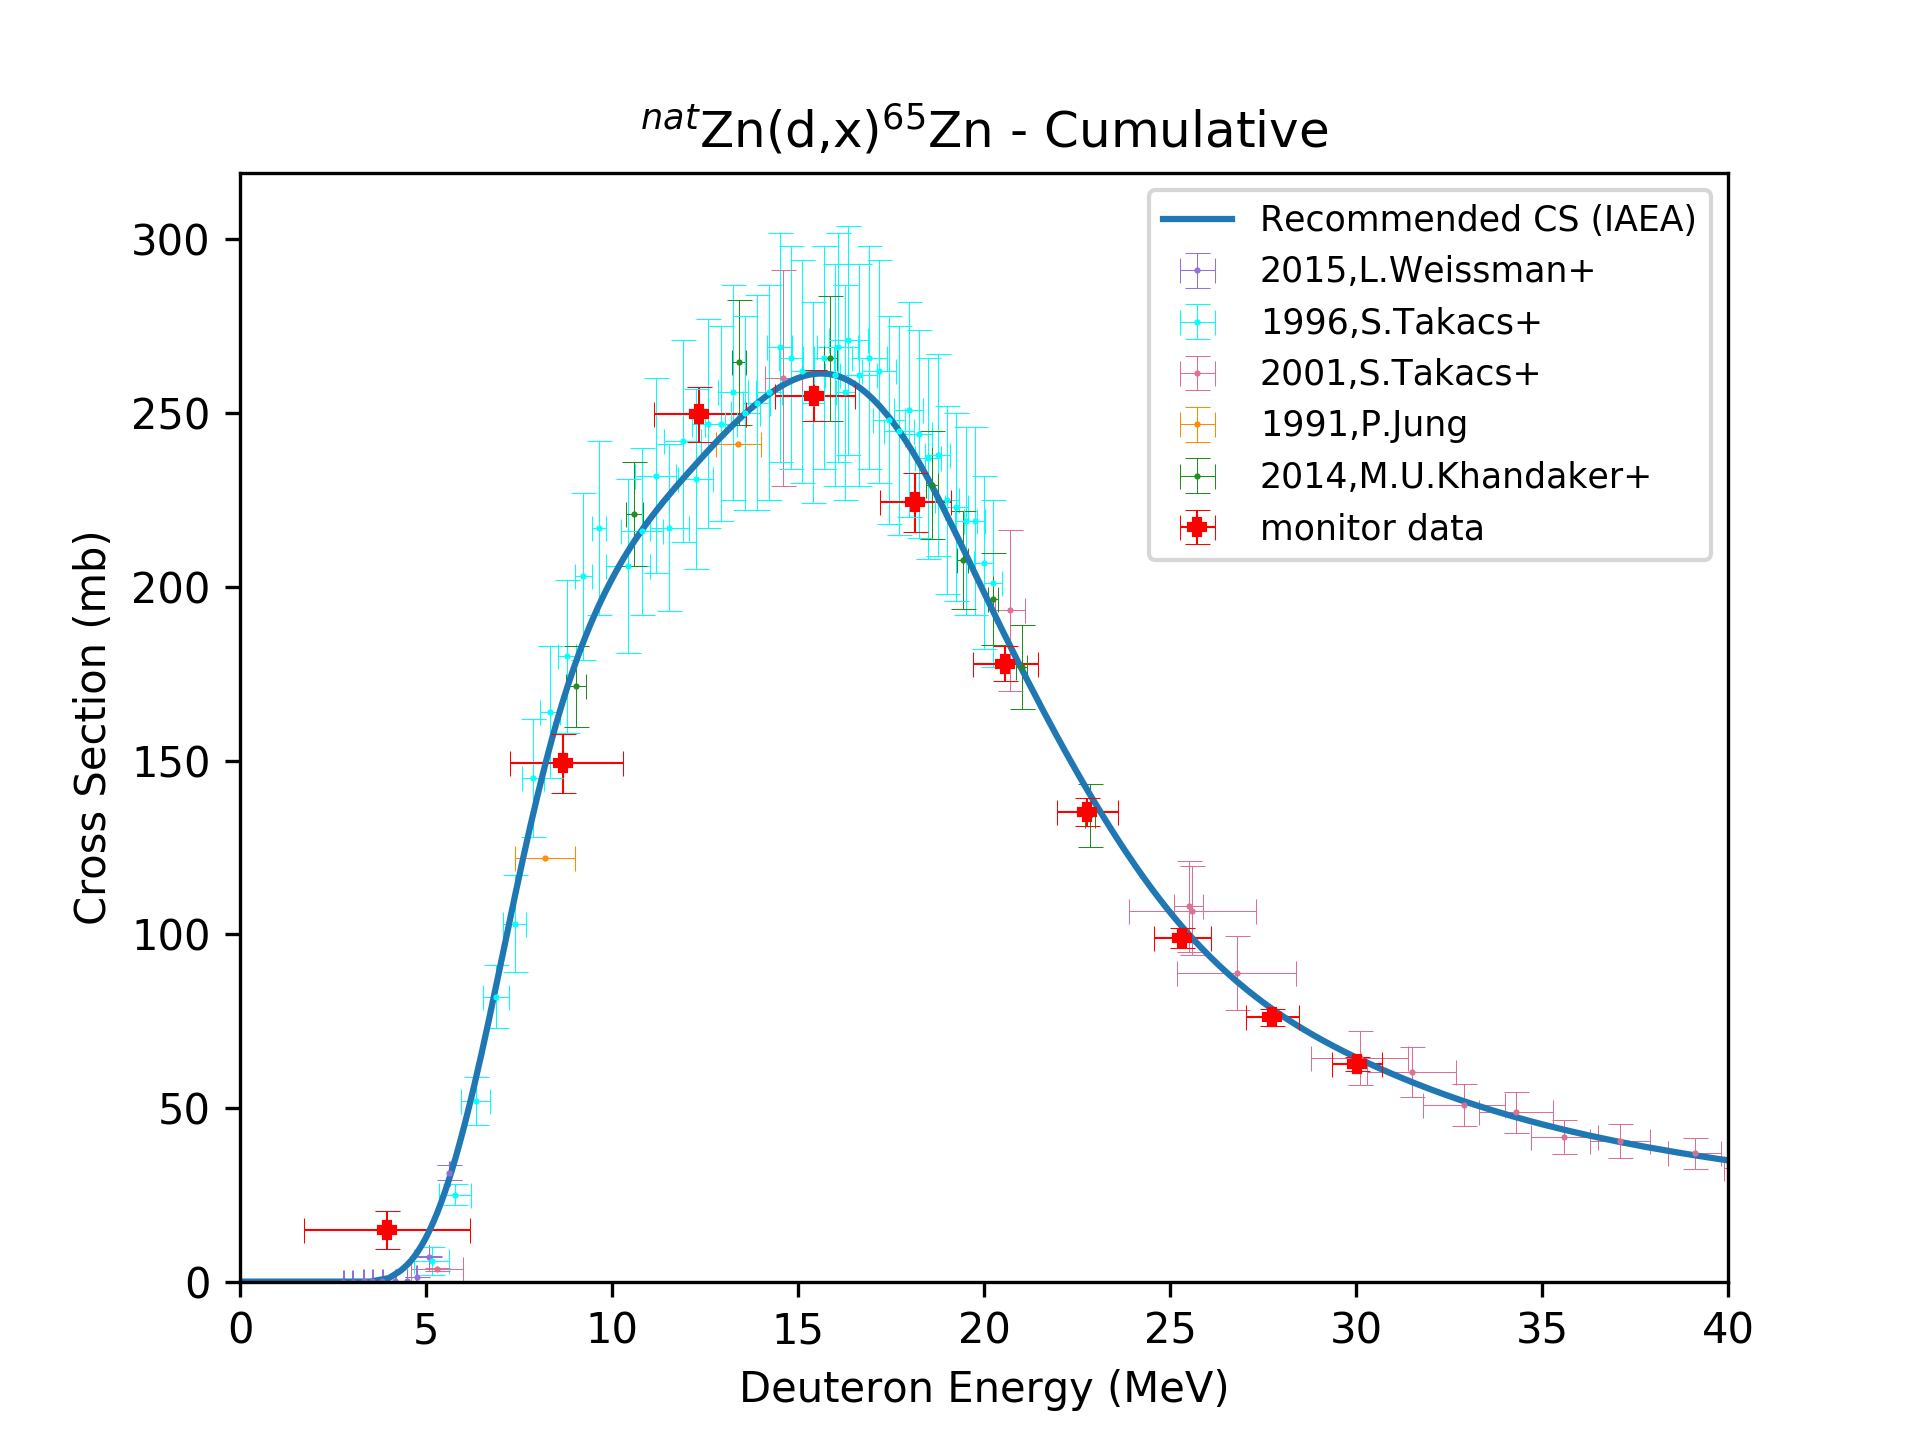
\includegraphics[width=5cm]{Cu_65Zn.png} }}%
    \quad
    \caption{Figure shows the estimation of monitor cross section using the calculated beam current. It is compared along with the monitor data.  }%
    \label{fig:monitor_BC}%
\end{figure}

\end{comment}

\chapter{Analysis}




The analysis of estimating production cross sections consisted of multiple steps. To obtain the end of beam activities the peak areas (number of counts) were found with gamma-ray spectroscopy using FitzPeaks\footnote{https://www.jimfitz.co.uk/fitzpeak.htm}. The efficiency calibration as a function of gammaray energy was done using $^{137}$Cs, $^{133}$Ba and $^{152}$Eu point sources. The energy degradation in the foils were simulated using NPAT\footnote{https://pypi.org/project/npat/}, giving the deuteron flux as a function of energy. Along with the simulation and IAEA recommened cross sections for the monitor reactions\footnote{https://www-nds.iaea.org/medical/monitor_reactions.html}, the weighted average beam current was estimated in each foil. 

\section{Gamma-ray spectroscopy}
The spectra were analyzed in FitzPeakz\footnote{https://www.jimfitz.co.uk/fitzpeak.htm}. The mathematic algorithm in which FitzPeakz is based upon is SAMPO80 \footnote{https://sci-hub.tw/https://doi.org/10.1016/0029-554X(81)90209-3}. \textcolor{blue}{The peaks are assumed Gaussian with an exponential tale on both sides of the peak. The exponential tale and Gaussian function are joined so function and first derivative are continous. The algorithm searches for peaks by using the smooth second difference (derivative?) Particularly good for detecting small peaks on a high or low background. The peak areas are calculated by fitting the precalibrated modified Gaussian to the data with a weighted least squares formula using a parabolic background. Fitting intervals are determined automatically by the program. Peaks separarated by less than 4 times the average fwhm are fitted together. }

For each spectra,  a report file containing peak energy, centre channel, full width half maximum, significance, goodness of fit, peak area, uncertainty in peak area, gammas per second, uncertainty in gammas per second and a background estimation for each peak was provided. The most important parameters were the energy, the peak area $N_C$ and uncertainty in peak area. Peak area was needed for the activity calculation in equation \ref{eq:Final_Expression_A0} which is an important parameter in the calculation of the cross section (equation \ref{eq:experimental_CS}), and in the calculation of the efficiency for the calibration sources (equation \ref{eq:efficiency_analytical}). Gammas per second (also called countrate) was used to get an indication if the rate of gammas, which were used as a critical tool to evaluate background contamination in a peak for instance. 

Figure \ref{fig:gammarayspectrum_example} shows an example of a gamma ray spectrum for one of the iridium spectra (Ir05) approximately 35 hours after end of beam. Figure \ref{fig:193mPt_spectra} shows the X-ray region and gamma region of $^{193m}$Pt. 

The nuclei were identified on behalf of thei're gamma-ray energy. The feeding of multiple nuclei into one gamma-ray peak was avoided by using other gamma-lines. 

\begin{figure}
    \centering
    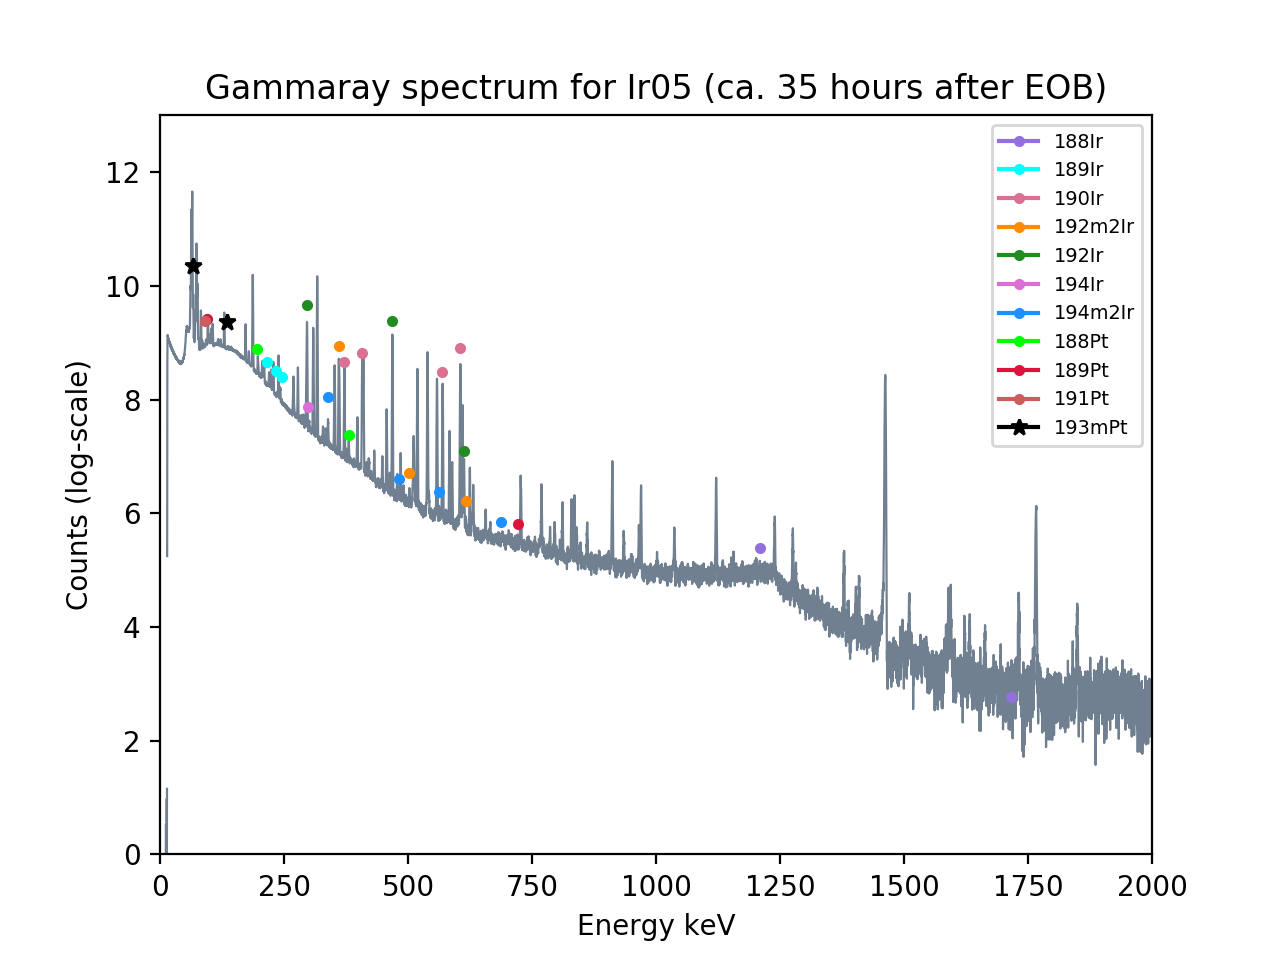
\includegraphics{Analysis/gammaray_spec_Ir05.png}
    \caption{Gammaray spectrum for Ir05 taken approximately 35 hours after end of beam. Nuclei does not necessarily represent what is present in the spectrum, but where the peak would have been. Hard to include all since there are different decay times. }
    \label{fig:gammarayspectrum_example}
\end{figure}


\begin{figure}%
    \centering
    \subfloat[X ray plot of 193mPt. ]{{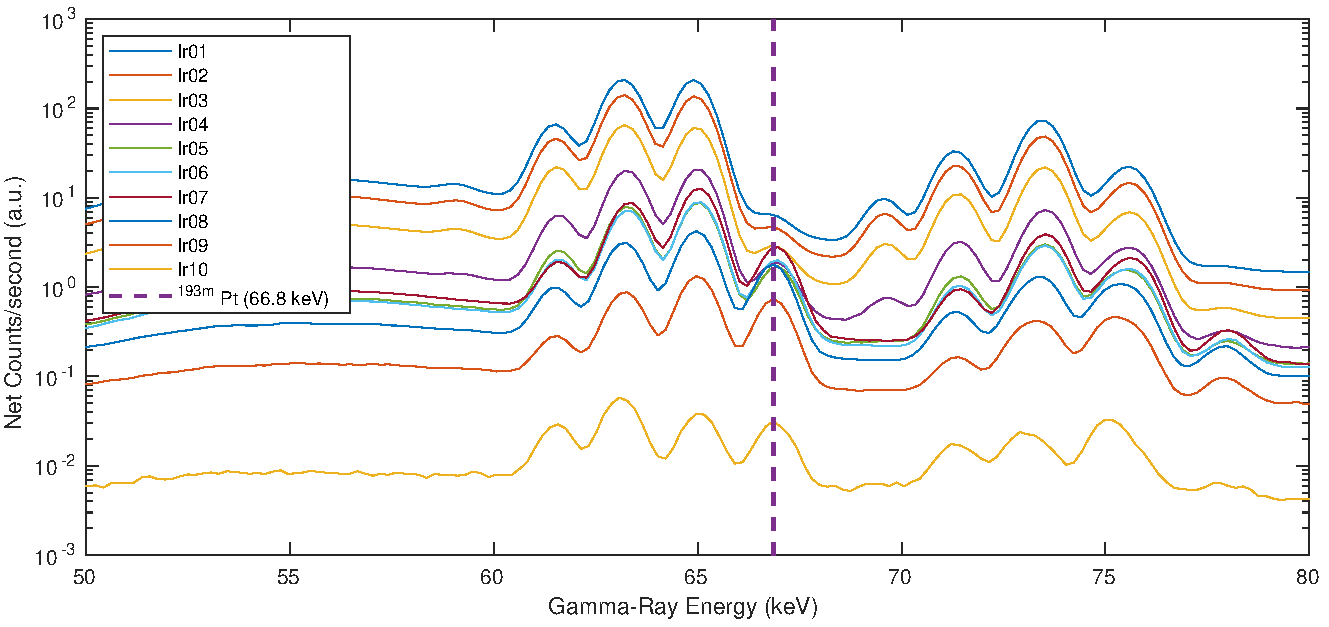
\includegraphics[width=10cm]{Analysis/193mPt_xray_plot.pdf} }}%
    \quad
    \subfloat[Gammaplot of 193mPt]{{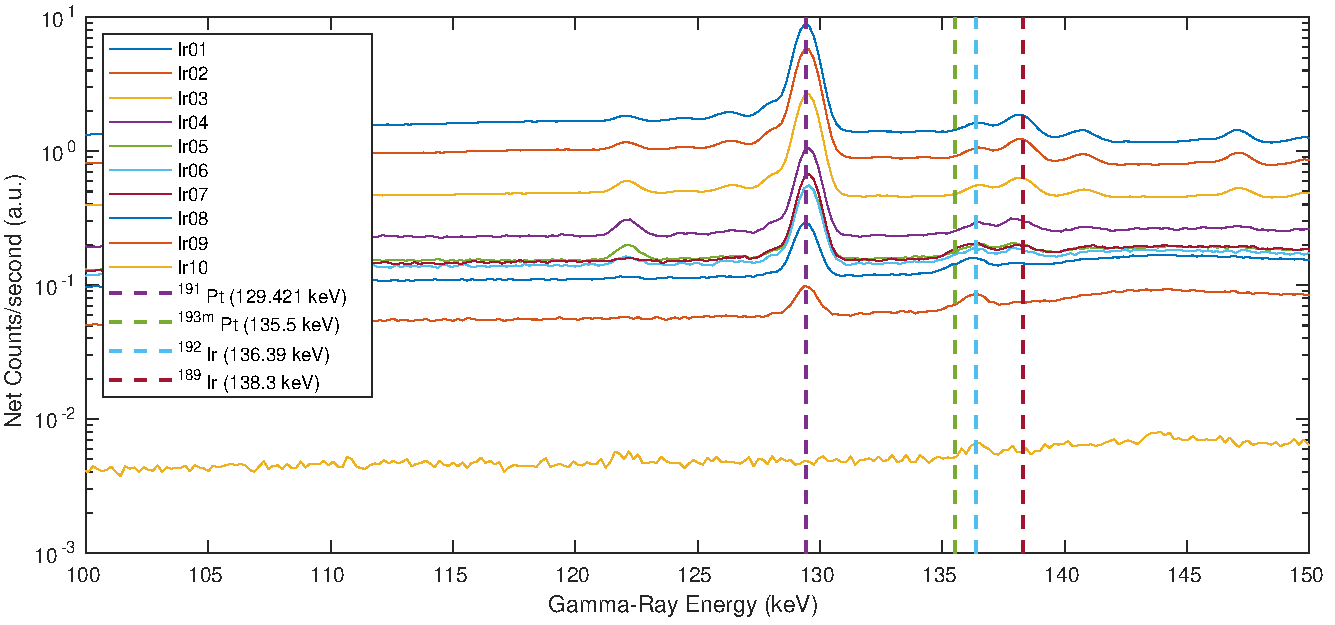
\includegraphics[width=10cm]{Analysis/193mPt_gamma_plot.pdf} }}%
    \caption{\textcolor{red}{Which spectra are these??  }}%
    \label{fig:193mPt_spectra}%
\end{figure}


\subsection{Energy and peak-shape calibration} \label{subsec:fitz_calibration}
Used calibration sources $^{137}$Cs ($t_{1/2}=30.08$ years\cite{Browne2007}), $^{133}$Ba ($t_{1/2}=10.551$ years\cite{Khazov2011}) and $^{152}$Eu ($t_{1/2}=13.517$ years\cite{Martin2013}), which can be seen on figure \ref{fig:calsources}.

\textcolor{blue}{The calculated peak locations and areas are finally corrected with energy and efficiency calibration data to yield peak energies and intensities. For the energy calibration, linear interpolation on a linear scale and for the efficiency calibration linear interpolation on a log-log scale are used in this code. Calibration errors are added to the peak location and intensity errors to give the final result (p.94). \\ The peak shape calibration uses 7 parameters; two background peaks, peak height and location, peak width, distance from peak centroid to the starting point of exponential on either side. The minimization of the least-squares expression to solve for the peak parameters is done by a subroutine package  with an iterative gradient algorithm utilizing the variable metric method. Minimization is terminated when all all components in the next step change by less than $10^{-8}$, if four succeeding values of $\chi^2$ are the same or if 100 iterations have been completed. The performed shape calibration can be checked with a few parameters, goodness of fit, $\chi^2$ per degree of freedom, sigma and error correlation. Sigma below 5 and error correlation between -1 and 1 are acceptable values.  (p.90)} \\


From the webpage\foonote{jim-fitz.com/calib.html}:
Each detector was calibrated with peak shape and energy for the calibration sources. Fitzpeakz takes in energy (.enc) and peak shape (.shp) calibration source files, containing the energies listed in table\ref{table:calibration_gammas}. For the peak shape, the program determines the parameters of width and the amount of low energy tailing. The energy calibration and peak shape calibration was estimated to a 1st order function. 




\section{Efficiency calibration} \label{sec:efficiency_calibration}
The efficiency calibration is an important factor in the calculation of the cross section in equation \ref{eq:experimental_CS}. The detector efficiency is the number of events registered divided by the events emitted by the source. The absolute efficiency can be divided into intrinsic and geometrical efficiency, where the intrinsic efficiency is the number of events registered divided by the number of events hitting the detector. The
intrinsic efficiency thus depends on the interaction cross section between incident particle and detector material. For neutral particles, the size of the detector affects the intrinsic efficiency, the larger crystal the larger the probability of interaction is. The geometrical efficiency is the radiation emitted by the source which hits the detector. (Techniques for Nuclear and Particle Physics Experiments. William R. Leo. Second Revised Edition. Springer.Verlag Berkling Heidelberg GmbH, New York (1994). p. 121-122 ) \\

\noindent 
The efficiency was measured using calibration point sources $^{137}$Cs ($t_{1/2}=30.08$ years\cite{Browne2007}), $^{133}$Ba ($t_{1/2}=10.551$ years\cite{Khazov2011}) and $^{152}$Eu ($t_{1/2}=13.517$ years\cite{Martin2013}). Figure \ref{fig:calsources} shows the calibration points sources ($^{22}$Na was excluded during the data-analysis since it only contains a single gamma-line and gave poorer results). On each calibration source, a reference date is given with an activity, which here is referenced to as $A_0$ of the calibration sources.\\

\noindent Solving Equation \ref{eq:Final_Expression_A0} for effiency, $\epsilon$, the analytical effiency as a function of gamma-ray energy and intensity is 
\begin{equation} \label{eq:efficiency_analytical}
    \epsilon(E_\gamma)= \frac{N_C \lambda}{A_0 I_\gamma (1-e^{-\lambda \Delta t_c})e^{-\lambda\Delta t_d}}
\end{equation}

where $\lambda$ is the decay constant and $N_C$ is the number of counts in the measured spectra, and $\Delta t_d$ is the delay time since the reference date. The analytical efficiency gives one single value for the efficiency at energy $E_\gamma$, but we want a continuous function which gives the effciency at any gamma-energy. A model based upon Gallagher, W. J., Cipolla, S.J. (1974) was applied which takes the probability of penetration through the deadlayer of the detector and the probability of interaction in the detector volume into account

\begin{equation} \label{eq:efficiency_estimated}
\epsilon(E_\gamma) =  B_0 + \underbrace{(e^{-B_1 E_\gamma^{B_2}})}_\text{dead layer}  \underbrace{(1-e^{-B_3 E_\gamma^{B_4}}))}_\text{interacting with volume} 
\end{equation}
\noindent 
where $B_i$ is optimum parameters minimizing the $\chi^2$ in the scipy optimizing curve fit function\footnote{https://docs.scipy.org/doc/scipy/reference/generated/scipy.optimize.curve_fit.html}). Figure \ref{fig:efficiency_curve} shows an example of an efficiency curve for a detector at a specific distance from the detector. The uncertainty of the efficiency was estimated using equation \ref{eq:variance_full} numerically. For each source, the gamma-lines with the intensities which were used to calculate the efficiency points for each source is listed in table \ref{table:calibration_gammas}. \\


\begin{figure}
    \centering
    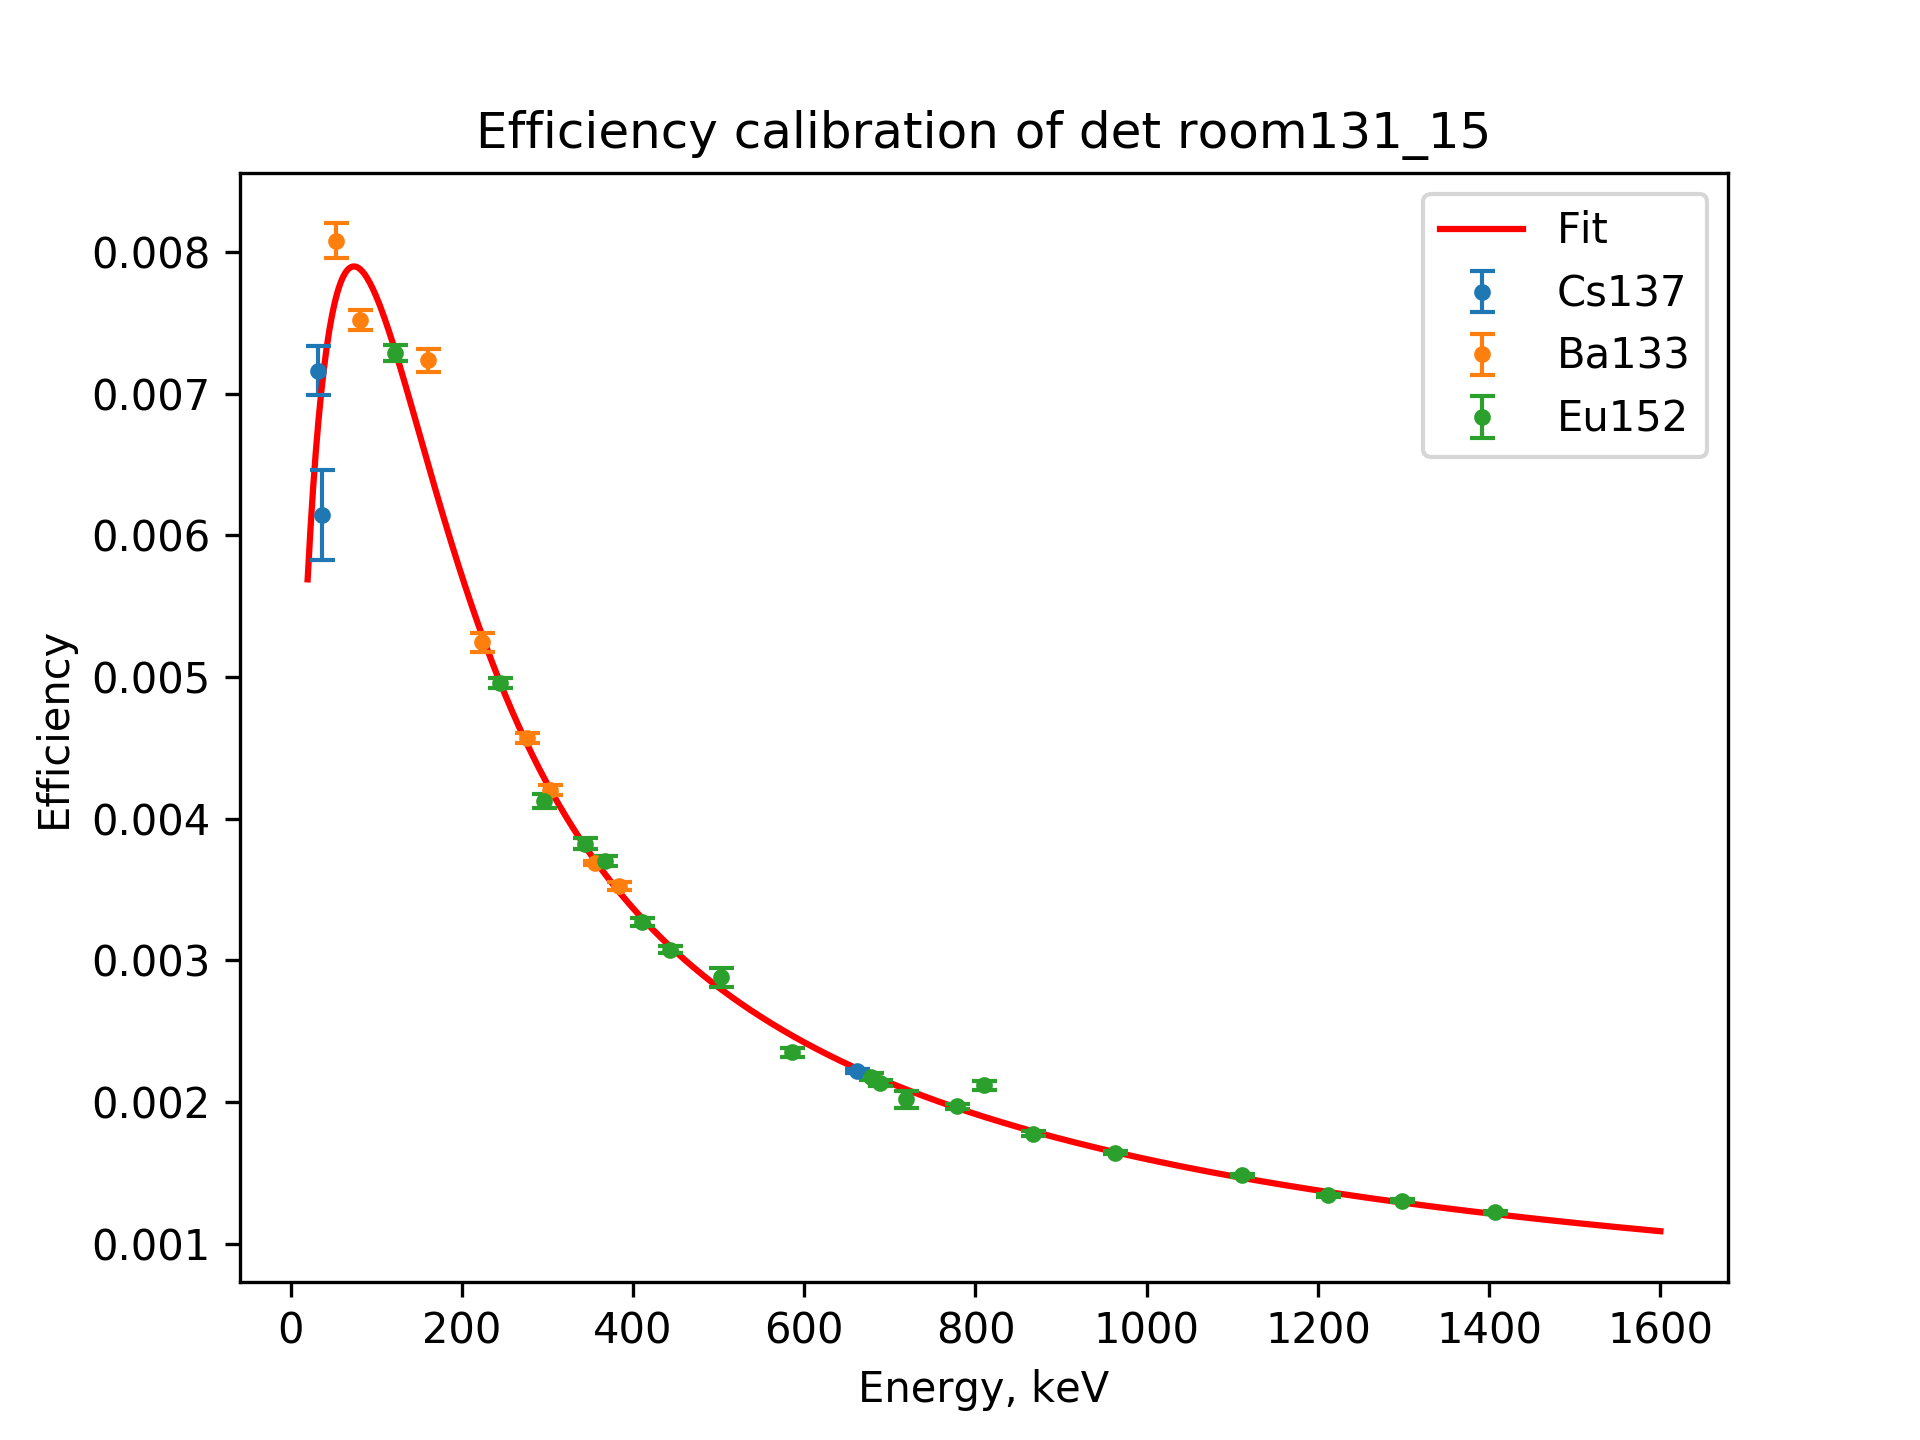
\includegraphics[width=0.6\textwidth]{Experiment/room131_15.png}
    \caption{An example of an efficiency curve with exact points calculated from equation \ref{eq:efficiency_analytical} and a curve fit from equation \ref{eq:efficiency_estimated}. }
    \label{fig:efficiency_curve}
\end{figure}

\section{End of beam activities}

The end of beam activities were estimated by extrapolating backwards in time, with the measured activities at various timepoints after the end of beam. The activities as a function of time sine EOB was calculated using equation \ref{eq:Final_Expression_A}, along with a self-attenuation correction: 

\begin{equation}
    A(\Delta t_d) = \frac{N_C\lambda}{\epsilon\I_\gamma (1-e^{-\lambda \Delta t_d})e^{-\mu\rho\Delta r/2}}
\end{equation}

where $\mu$ is the photoon attenuation coefficients from the XCOM photon cross section database+\footnote{https://www.nist.gov/pml/xcom-photon-cross-sections-database}, and $\rho\Delta r$ is the mass density of the foil. The gammas which were used are listed in tables \ref{tab:Products_Fe}, \ref{tab:Products_Ni}, \ref{tab:Products_Cu} and \ref{tab:Products_Ir} for iron, nickel, copper and iridium respectively. The gamma-ray self-attenuation (which is typically less than 0.2 \% (Iron paper, Andrew)) correction is based on the assumption that all activity that is made is located midway in the foil thicknesses. In reality however, the activity profile will follow the same shape as the excitation function over the energy range that expands over the foil, \textcolor{red}{if we assume that the stopping power dE/dx=0 which is a good estimation for thin foils less than 100 mg/cm$^2$??} (since activity and cross section are proportional). We do not know the excitation function ahead of time, and the excitation function does not change much either, since the foil thicknesses are so thin. So instead, this simplification is done, assuming that the average attenuation is through half of the foil thickness. \\ 

\noindent 
The equation describing the shape of the decay curve is given in equation \ref{eq:activity_decaylaw} for single decay or \ref{eq:ndecay_chains} for multiple decay. Decay chains of single and two-step decay (n=1,2) was sufficient in this analysis; 
\begin{equation} \label{eq:onestep_activity}
    A = A_0 e^{-\lambda \Delta t_d},\quad \text{ single step decay}
\end{equation}

and

\begin{equation} \label{eq:twostep_activity}
    A_2(t) = \lambda_n \Big[ A_{1,0}\lambda_1 \frac{(e^{-\lambda_1 } + e^{-\lambda_2})}{\lambda_1 - \lambda _2} + A_{2,0}e^{-\lambda_2 t} \Big],\quad \text{two step decay}
\end{equation}

where subnumber 1 is the parent nucleus, and subnumber 2 is the daughter nucleus. Parent activity is calculated from single step decay. The uncertainty was treated as \textcolor{red}{covarianced variables?} \\

The way in which the extrapolation was done was the scipy optimize curve fit function, where the $A_0$ of the daughter was the optimizing parameter. Since there is only one optimized parameter, there was no covariance and the uncertainty was calculated using equation \ref{eq:uncertainty_simplification}.  In the cases where neither parent or daughter activity were known, which were the case for the monitor reaction $^{58}Co$ with $^{58m}$Co decaying into the ground state by internal conversion, both parent and daughter activity were optimizing parameters which are very correlated and thus the uncertainty in end of beam activity was calculated \ref{eq:variance_full}. Figure \ref{fig:activity_curves} shows two examples of the two different activity curves; one step decay for $^{193m}$Pt ($t_{1/2}$=4.33 days) and two step decay for the monitor product $^{58}$Co ($t_{1/2}$=70.86 days) with feeding from the isomer $^{58m}$Co ($t_{1/2}$=9.10 hours).  


\begin{figure}%
    \centering
    \subfloat[Activity of $^{193m}$Pt ($t_{1/2}$=4.33 d) produced from iridium. The end of beam activity was estimated using a one step decay (equation \ref{eq:onestep_activity})]{{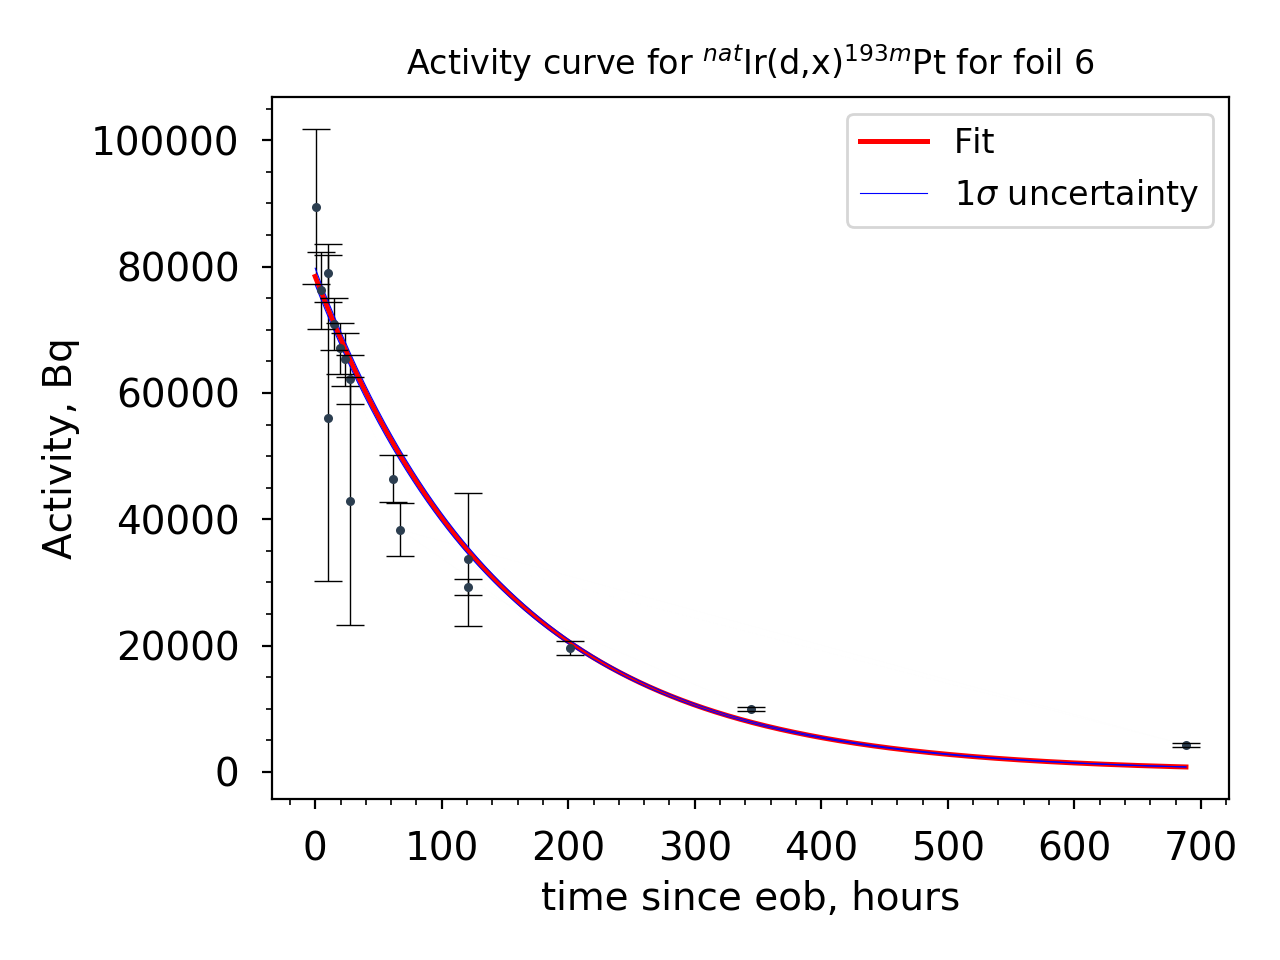
\includegraphics[width=11cm]{Analysis/activity_Ir_193mPt_f6.png} }}\hfill
    \subfloat[Activity of $^{58}$Co ($t_{1/2}$=70.86 d) produced from nickel. The end of beam activity is estimated using a two step decay (equation \ref{eq:twostep_activity}. The feeding is from $^{58m}$Co ($t_{1/2}$=9.10 h.) ]{{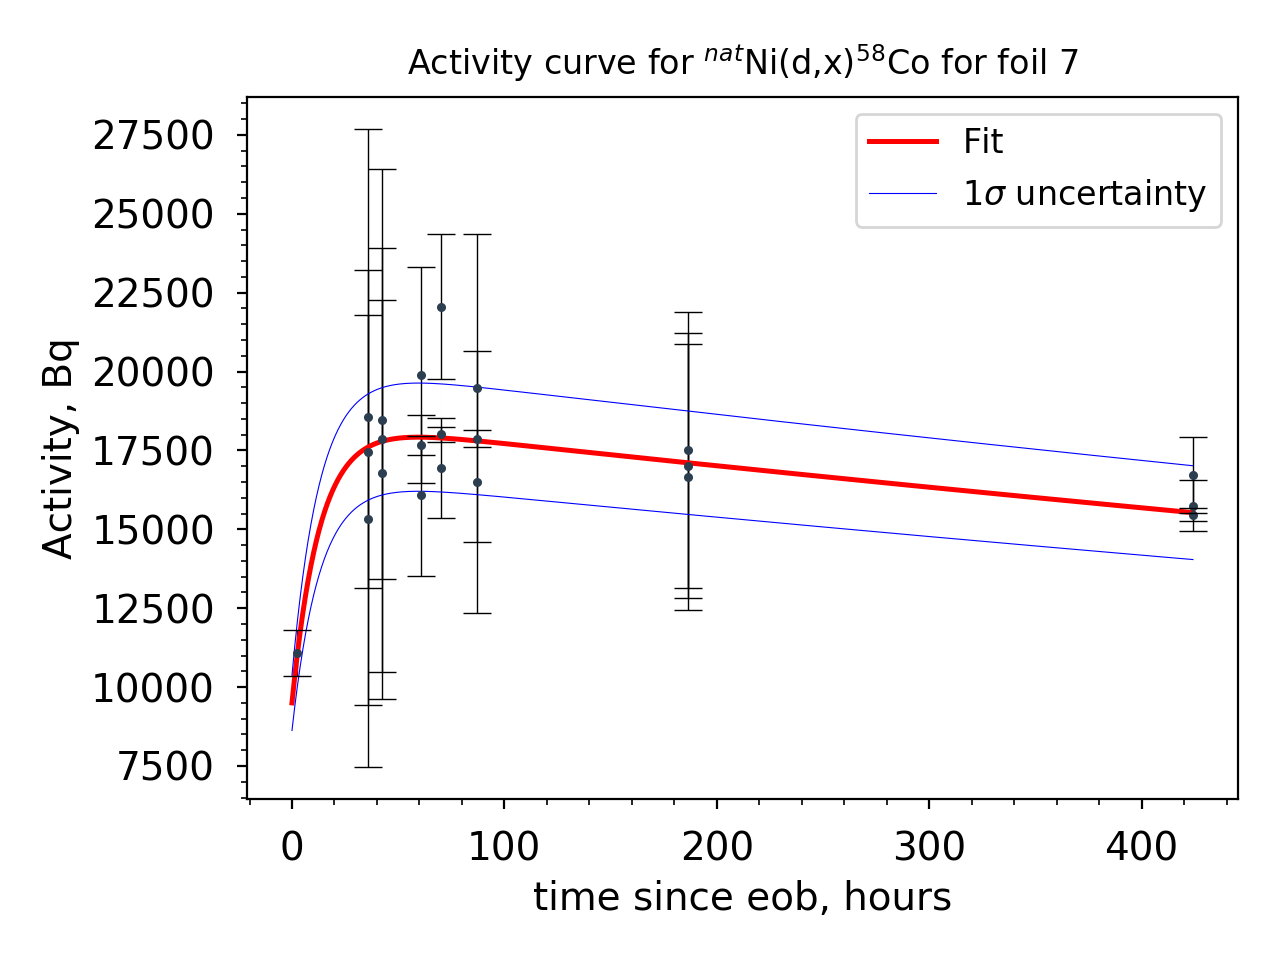
\includegraphics[width=11cm]{Analysis/activity_Ni_56Co_f7.png} }}%
    \caption{Two examples of activity curves. The uncertainty in activity decreases with increasing time since end of beam which is due to longer counts decreases the uncertainty. (from theory, counting statistics)  }%
    \label{fig:activity_curves}%
    
\end{figure}



\section{Estimation of the beam current}
The beamintegrator measured a current of 128.5 nA in front of the beam stack. However in order to have precise cross section measurements, the beamcurrent in each foil was estimated. The IAEA recommended monitor reactions (2017) $^\text{nat}$Ni(d,x)$^{61}$Cu,$56,58$Co, $^\text{nat}$Cu(d,x)$^{62,63,65}$Zn and $^\text{nat}$Fe(d,x)$^{56}$Co were used to obtain a weighted average beam current in each foil solving equation \ref{eq:Final_Expression_A0} for beam current $\Phi$:

\begin{equation} \label{eq:BC_simple}
    \Phi(E) = \frac{A_0}{N_T \sigma(E)_\text{mon}(1-e^{-\lambda \Delta t_\text{irr}})}
\end{equation}

Equation \ref{eq:BC_simple} builds upon the thin target assumption, which implies that the energy degradation dE/dx=0. However, we know that there is an energy distribution, which was estimated using NPAT's (Nuclear Physics Analysis Tool) Ziegler simulation. The ziegler code simulates the deuteron transport based upon the Anderson \& Ziegler stoppingpower formalism, using Monte Carlo simulations \textcolor{red}{write a few sentences in theory..}. The code provides the full deuteron energy and flux degradation in each foil, $d\phi/dE$, which can be visualized for the iridium foils in figure \ref{fig:ir_energyflux}.  Can be seen that as the deuteron energy is degraded, the mean value is shifted towards the low energy side, and the the peak width increases. As stoppingpower is inversely proportional to the charge particle energy ($-\frac{dE}{dx}\propto \frac{1}{\beta^2}$, bethe block), and along with scattering taking place towards the end of stack, the low energy tail is more degraded, and we see a skew towards the low energy, creating a broader energy-flux profile and a shift of the mean value (centroid). This shift leads to an increasing uncertainty in energy. The (normalized) flux-weighted average energy for each foil was calculated, \textcolor{blue}{ironpaper: which takes into account the slowing down of of deuterons, and reports effective energy centroid of each foil}, using the energy distributions $d\phi/dE$ provided by the Ziegler code:

\begin{equation} \label{eq:flux_weighted_average_energy}
    \langle E \rangle = \frac{\int E \frac{d\phi}{dE}dE}{\int \frac{d\phi}{dE}dE}
\end{equation}

The uncertainty in beam energy is divided into low energy and high energy tale, with the FWHM split by the centroid (figure \ref{fig:ir_energyflux}). 

Likewise, the energydependent monitor IAEA cross sections need to be flux-weighted over each foil. In order to do this, a spline interpolation over the energy array over each foil provided by the Ziegler simulation was spline interpolated with the IAEA recommended cross section data. Thus, the monitor cross section in equation \ref{eq:BC_simple} is modified to 

\begin{equation}
    \sigma (\langle E\rangle) = \frac{\int \sigma_\text{mon} \frac{d\phi}{dE}dE}{\int \frac{d\phi}{dE}dE}
\end{equation}


\begin{figure}
    \centering
    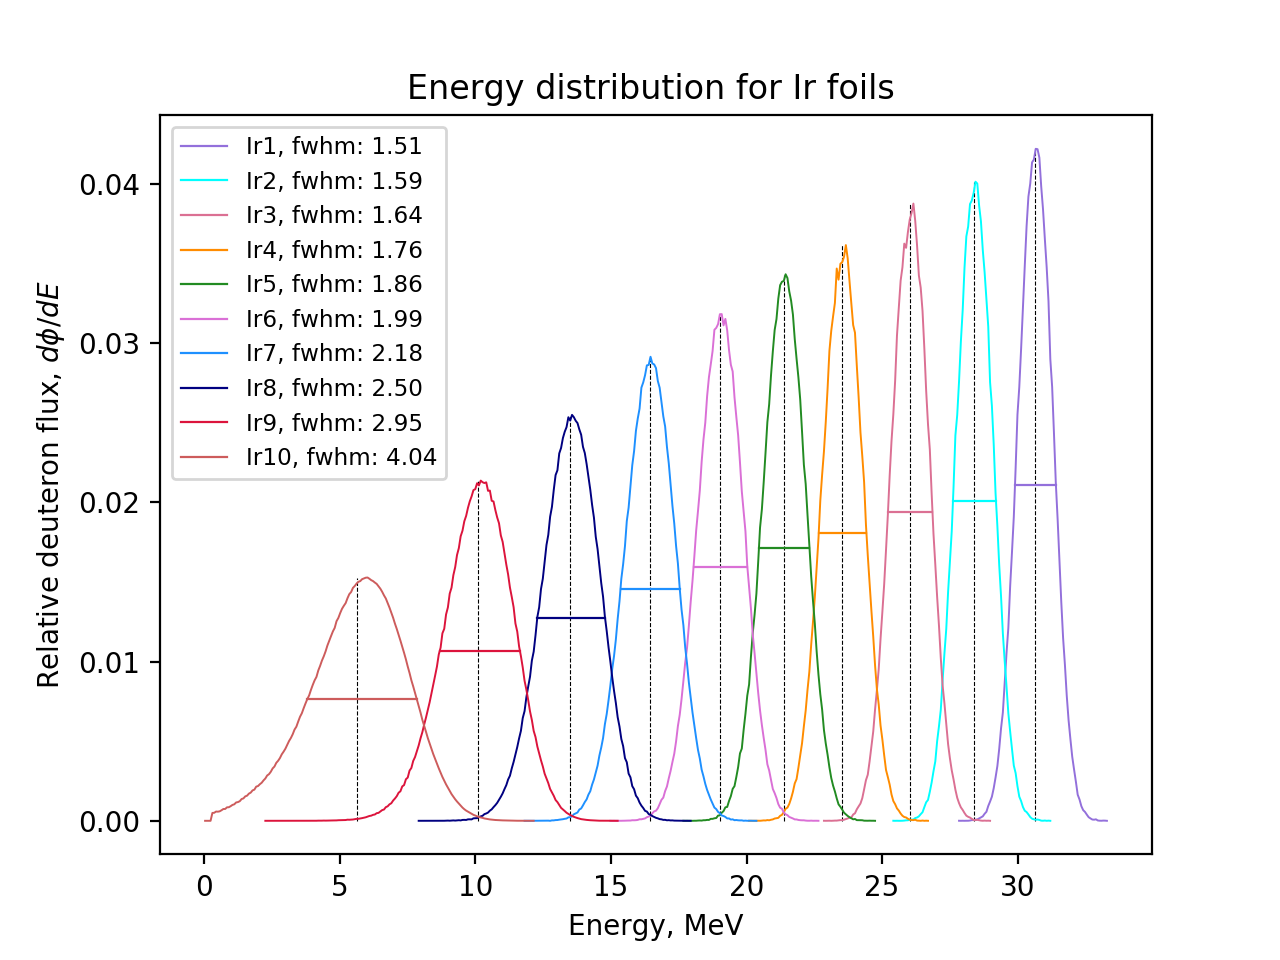
\includegraphics{Analysis/Ir_flux_distribution_B_+2_D_+4,25.png}
    \caption{Iridium energy flux distribution over the 10 foils. As the energy degrades, scewed and larger full width half max. The vertical line in each peak is the mean value. This indicates that at lower energies, the right uncertainty is greater than the left uncertainty in the peak.}
    \label{fig:ir_energyflux}
\end{figure}

With the end of beam activities for the monitor reactions, number of target nuclei and the flux- weighted IAEA cross sections, the beam current as a function of the flux-weighted average beam energy was estimated for each reaction in each foil. 

\subsection{Variance minimization of the deuteron transport calculations}
In theory, the estimated beam current of a charge particle beam should be constant, until completely stopped, since the majority of the incident particles does not interact in nuclear reactions, but only lose energy via elastic and inelastic scattering. However, non-consistant values of the beam current, especially in the back of the stack can be due to energy bins being assigned wrongly in the energy distribution simulation done in Ziegler or a systematic error in the areal density which gets progressively worse further back in the stack (Niobium paper, Andrew). A way to work around these errors was to perform a variance minimization varying the beam energy and the areal density of the foils with 20\% increase and decrease systematically, and estimate the reduced $\chi^2$ (equation \ref{eq:chisq_DOF}) over compartment 3,6 and 9. Variance minimization (Andrew's Niobium and iron paper + \foonote{https://sci-hub.tw/https://doi.org/10.1016/j.nimb.2016.09.018}). \\

 For compartment 3 ($E_d$=25 MeV) all seven monitor reactions were above threshold,  thus 6 degrees of freedom.  However,  early in the target stack,  the scattering was low, and the $\chi^2$ does not tell how well the energy bin assignment work further back in the stack.  For compartment 6 ($E_d$=18 MeV), all the six possible monitor reactions (for nickel and copper) were above threshold, and it gave a good estimate of how the beam current was developing throughout the stack.  In compartment 9 ($E_d$=10 MeV), five monitor reactions are above threshold (except for $^{62}$Zn).  At the very end it is possible to see the full effect of the scattering.\\

With the assumption that the beamcurrent loss is zero over one compartment, a linear fit-model (using the scipy optimize curvefit function) with a slope equal to zero was used to estimate the beam current in each compartment, and with the estimated $\chiˆ2$.  

Figure \ref{fig:BC_comp6} shows the uncertainty weighted linear fit over compartment 6. 

\begin{figure}
    \centering
    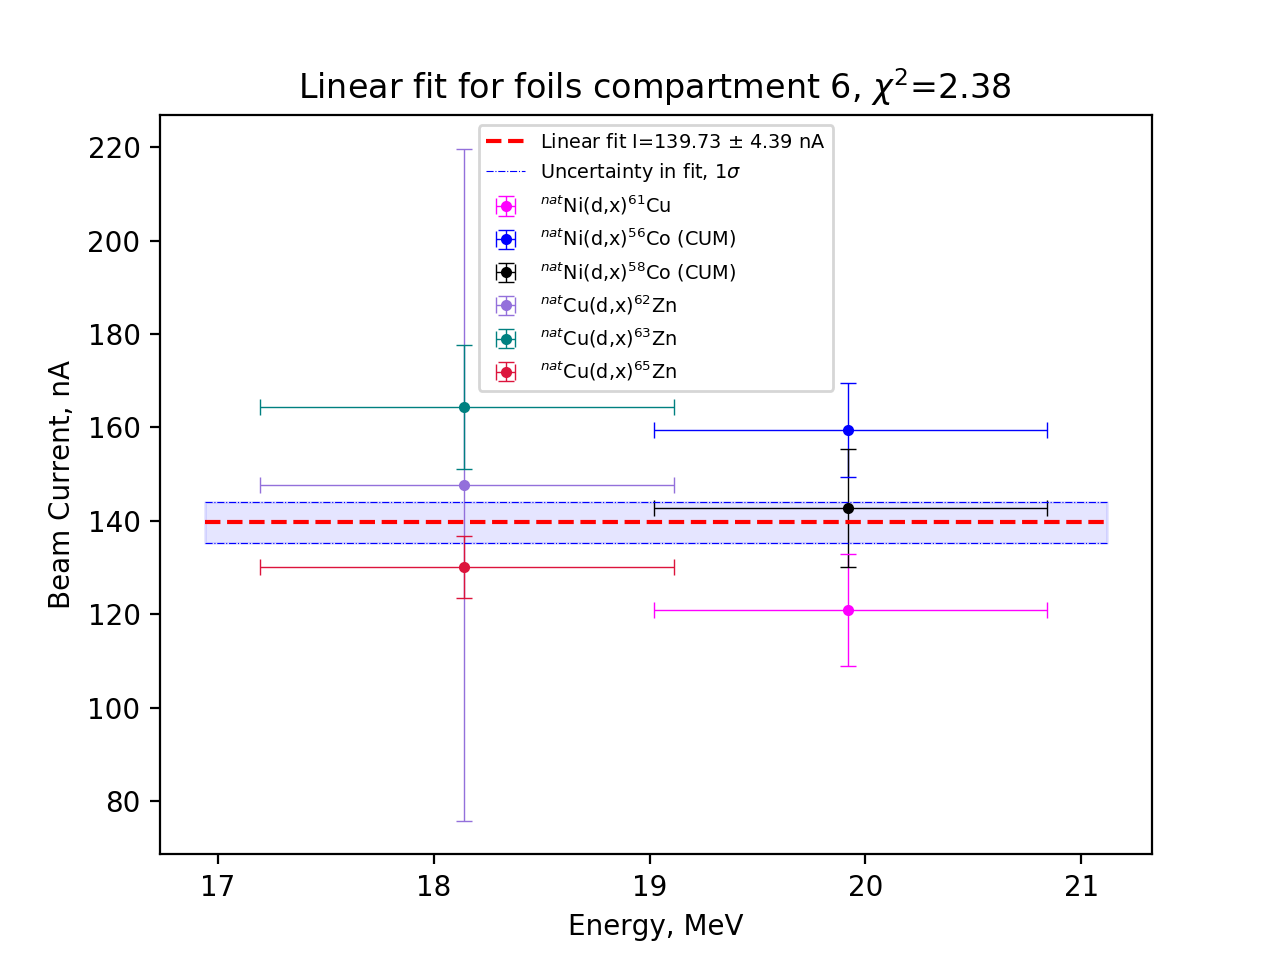
\includegraphics{Analysis/Compartment_6.png}
    \caption{The estimated (uncertainty weighted) beamcurrent over compartment 6. }
    \label{fig:BC_comp6}
\end{figure}

Figure \ref{fig:varmin_beamcurrent} shows the beam current before and after variance minimization, and the weighted average beam currents are listed in table \ref{tab:weighted_BC} estimated before and after the variance minimization. After variance minimization, the beam current estimated in each compartment (stabled lines) were similar, and meanwhile the weighted $\chi^2$ was about the same in compartment 6, it has improved in compartment 3 and very visible in compartment 9. In general the points are also more aligned. 

\begin{figure}%
    \centering
    \subfloat[]{{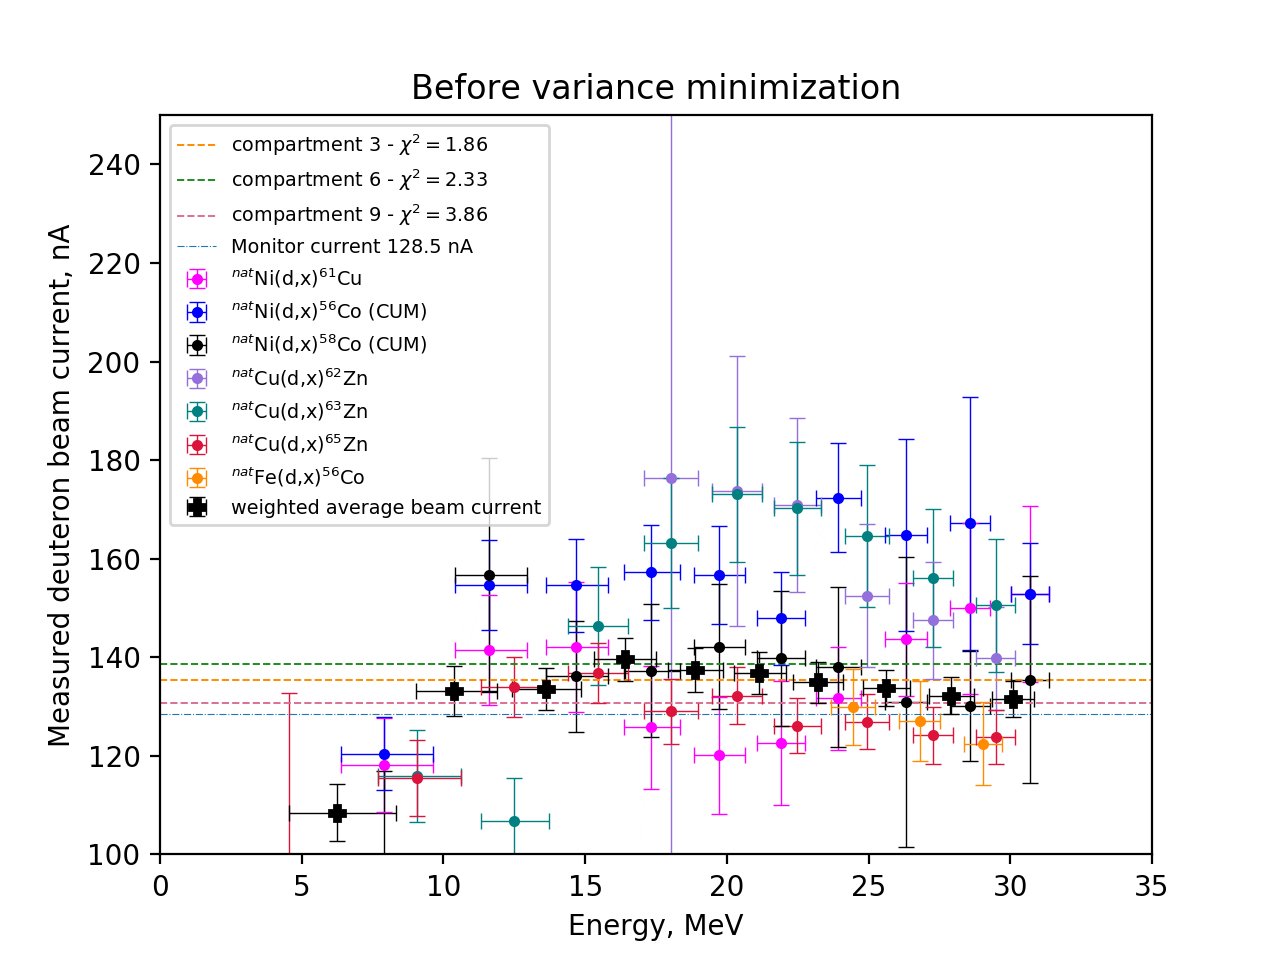
\includegraphics[width=11cm]{Analysis/beamcurrent_B_0_D_0.png} }}\hfill
    \subfloat[A 2\% increase in beam current and a 4.25\% increase in areal density gave the overall most consistent beam current, with reasonable values for the weighted . ]{{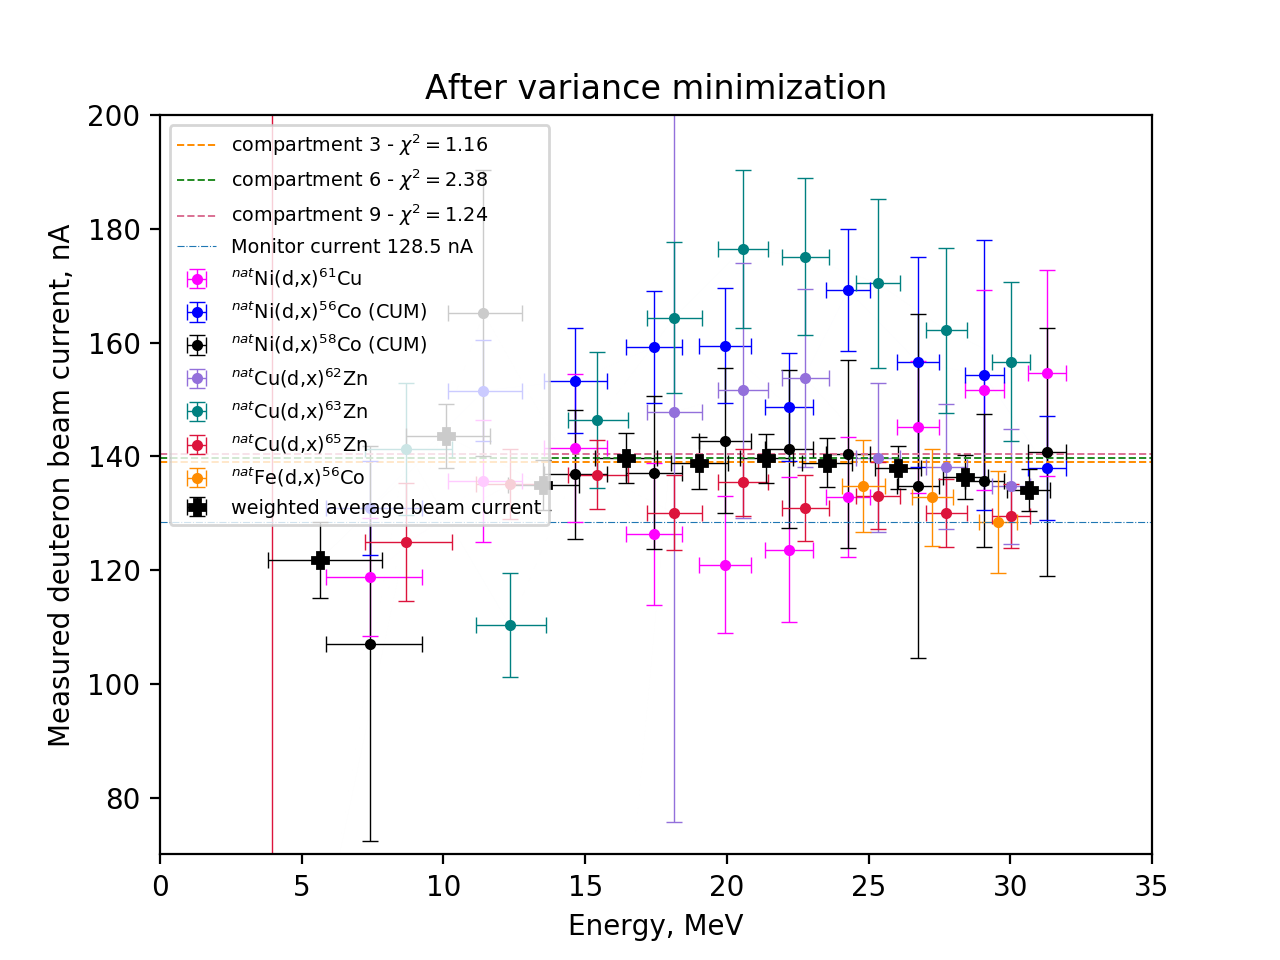
\includegraphics[width=11cm]{Analysis/beamcurrent_B_+2_D_+4,25.png} }}%
    \caption{Beam current before and after variance minimization.  }%
    \label{fig:varmin_beamcurrent}%
\end{figure}

\begin{table}[]
    \centering
        \caption{The weighted average beam current before and after variance minimization in each compartment. The beam current on the 88-Inch Cyclotron beam integrator was 128.5 nA.}
    %\footnotesize
    \begin{tabular}{c |c c}
        \hline 
       Compartment & \makecell{Before} & \makecell{After}\\ 
        \hline 
        \makecell{01} & \makecell{131.56 \pm 3.64} & \makecell{134.08 \pm 3.70}  \\ 
        \makecell{02} & \makecell{132.23 \pm 3.74} & \makecell{136.42 \pm 3.83} \\ 
        \makecell{03} & \makecell{133.81 \pm 3.64 } & \makecell{138.02 \pm 3.75} \\ 
        \makecell{04} & \makecell{134.89 \pm 4.21 } &  \makecell{138.88 \pm 4.31}\\ 
        \makecell{05} &\makecell{136.85 \pm 4.21} & \makecell{139.67 \pm 4.29} \\
        \makecell{06} &\makecell{137.40 \pm 4.53} & \makecell{138.85 \pm 4.58} \\
        \makecell{07} &\makecell{139.55 \pm 4.37} & \makecell{139.77 \pm 4.37} \\
        \makecell{08} &\makecell{133.60 \pm 4.27} & \makecell{134.96 \pm 4.32}\\
        \makecell{09} &\makecell{133.16 \pm 5.04} & \makecell{143.59 \pm 5.67} \\
        \makecell{10} &\makecell{108.49 \pm 5.80} & \makecell{121.75 \pm 6.65} \\
    
         %\makecell{Before} & \makecell{131.56 \pm 3.64} & \makecell{132.23 \pm 3.74} & \makecell{133.81\pm3.64 } & \makecell{134.89\pm 4.21 } & \makecell{136.85_{\pm 4.21}} & \makecell{137.40 \pm 4.53} & \makecell{139.55 \pm 4.37} & \makecell{133.60 \pm 4.27} & \makecell{133.16 \pm 5.04} & \makecell{108.49 \pm 5.80}  \\
         %\makecell{After} & \\
    \end{tabular}
    \label{tab:weighted_BC}
\end{table}

\begin{comment}
\section{Energy and Beam current}



For the equation for cross section (equation \ref{eq:cross_section_equation}), the beam current $\Phi(E)$ must be known. The beam integrator measured 128.5 nA, which is the current entering the stack. However, due to large energy degradation in the energy stack, there will be a certain spread of the beam, following scattering. In addition, there have not been an experiment with deuterium on a target stack before, so we also needed to see how much deuteron break up affected the current throughout the stack. Monitor reactions are reactions with well-known cross sections\footnote{https://www-nds.iaea.org/medical/monitor_reaction_article.pdf}. The IAEA recommended cross sections for $^\text{nat}$Fe(d,x)$^{56}$Co, $^\text{nat}$Ni(d,x)$^{61}$Cu, $^\text{nat}$Ni(d,x)$^{56,58}$Co and $^\text{nat}$Cu(d,x)$^{62,63,65}$Zn (\textcolor{red}{write about Q value, half life}) were used to estimate a more sensitive deuteron beam current throughout the stack. By solving \ref{eq:cross_section_equation} for beam current, the beamcurrent throughout the stack can be estimated

\begin{equation}
    \Phi(E) = \frac{A_0}{N_T (1-e^{-\lambda \Delta t_\text{irr}})\sigma(E)_\text{mon}}
\end{equation}

In cross section experiments using thin targets\footnote{Special curriculum p. 14}, the suggested value is a flux average cross section, which implies that the cross section is dependent on the flux-weighted average beam energy. One single foil thus provides one cross section measurement, with the uncertainty in energy only being dependent on the energy distribution in each foil. For thin targets, a stopping power $dE/dx=0$ is assumed which is a very good approximation for targets which are less than 50 mg/cm$^2$ \textcolor{red}{cite?}.   

Normalized differential beam current  (\textcolor{red}{need some help understanding this in detail})
\begin{equation}
    \sigma(E)_\text{mon}=\frac{\int \sigma(E)\frac{d\phi}{dE}dE}{\int \frac{d\phi}{dE}dE}
\end{equation}

\textcolor{blue}{From niobium paper: Since stoppingpower is inversely proportional for to cp energy, the low energy tail of the energy distribution is degraded more in each stack element than the high energy tail. This effect compounds to towards the rear of the stack, creating a significantly broadened low energy tail, and a progressevely larger net shift of the centroid to a lower energy. To account for this increasing energy uncertainty, a suitably representative energy must be established for each foil of the target stack. The flux weighted average deuteron energy in each foil $\langle E \rangle$ represents the energy centroid for deuterions in a target stack using the energy distributions from $d\phi/dE$ from the Ziegler stopping power deuterion transport }
\begin{equation}
    \langle E \rangle = \frac{\int E \frac{d\phi}{dE}dE}{\int \frac{d\phi}{dE}dE}
\end{equation}

where $\sigma(E)$ is the IAEA recommended cross section, $\frac{d\phi}{dE}$ is the energy dependent deuteron flux through each foil. The deuteron flux (or energy degradation) was estimated using a code called NPAT's (nuclear physics analysis tool) Ziegler simulation\footnote{https://pypi.org/project/npat/}. NPAT uses the Anderson \& Ziegler formalism for calculating charged-particle stopping powers in matter in a stack with targets. \textcolor{red}{write a few sentences about this in the theory!}. The code thus simulates the deuteron flux as a function of energy in the beam stack (assigned to a foil).

Figure \ref{fig:ir_energyflux} shows an overview of the flux-energy distribution in each foil for Iridium. The other monitor foils have the same functions.  \textcolor{red}{Write about recommended data, the spline function etc etc.. }

\begin{figure}
    \centering
    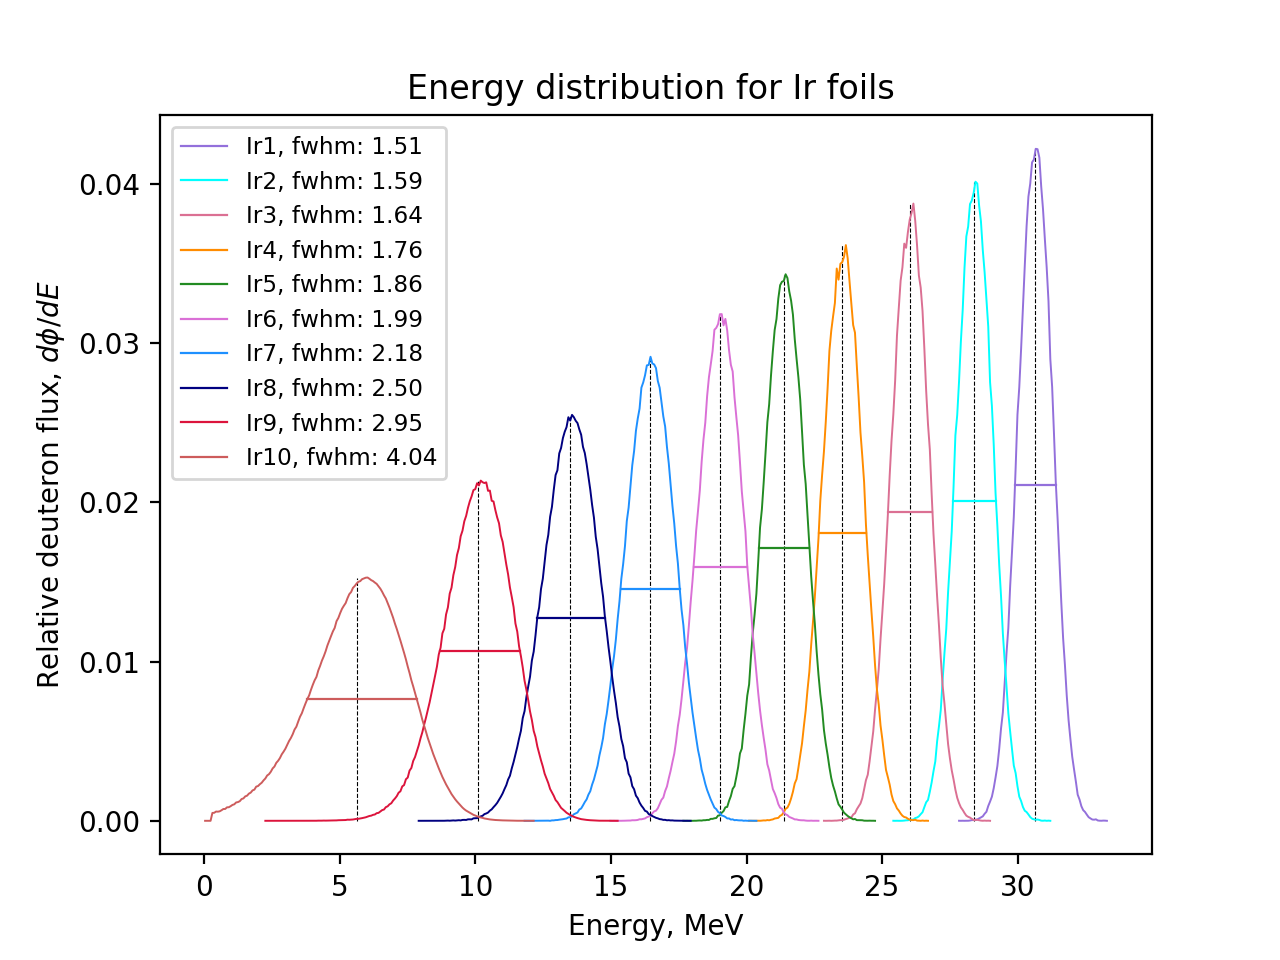
\includegraphics{Analysis/Ir_flux_distribution_B_+2_D_+4,25.png}
    \caption{Iridium energy flux distribution over the 10 foils. As the energy degrades, scewed and larger full width half max. The vertical line in each peak is the mean value. This indicates that at lower energies, the right uncertainty is greater than the left uncertainty in the peak.}
    \label{fig:ir_energyflux}
\end{figure}

\textcolor{red}{need some info from andrew here}

\subsection{Variance minimization}
\textcolor{blue}{From Niobium paper p. 57: In theory, the beam current should be more or less constant through the stack, even though the deuterons lose energy. Variance minimization is a technique to reduce the uncertainty in the deuteron beam energies. Non-consistent values  for the beam current further back in the stack can be wrong energy bin assignments in the modeled energy distribution (ziegler), or a systematic error in the areal density, which gets progressively worse further back in the stack, "due to the compound effect of systematic uncertainties in stack areal densities"}. The areal density and the beam energy was varied with 20\% increase and decrease, and the reduced $\chi^2$ (equation \ref{eq:chisq_DOF}) was estimated over compartment 3, 6 and 9. For compartment 3 ($E_d\simeq$25 MeV) all seven monitor reactions were above threshold, thus 6 degrees of freedom. However, early in the target stack, the scattering was low, and the $\chi^2$ does not tell how well the energy bin assignment work further back in the stack. For compartment 6 ($E_d\simeq$18 MeV), all the six possible monitor reactions (from nickel and copper) were above threshold, and it gave a good estimate of how the beam current was developing throughout the stack. In compartment 9 ($E_d\simeq$10 MeV), five monitor reactions are above threshold (except for $^{62}$Zn). At the very end it is possible to see the full effect of the scattering. \\

\noindent 
The beamcurrent loss is assumed zero in one compartment, so a linear beam current fit would have a slope equal to zero. The estimated beam current in each compartment was estimated using the scipy curve fit function, with a straight line as model. Figure \ref{fig:BC_comp6} shows the uncertainty weighted linear fit over compartment 6. 

\begin{figure}
    \centering
    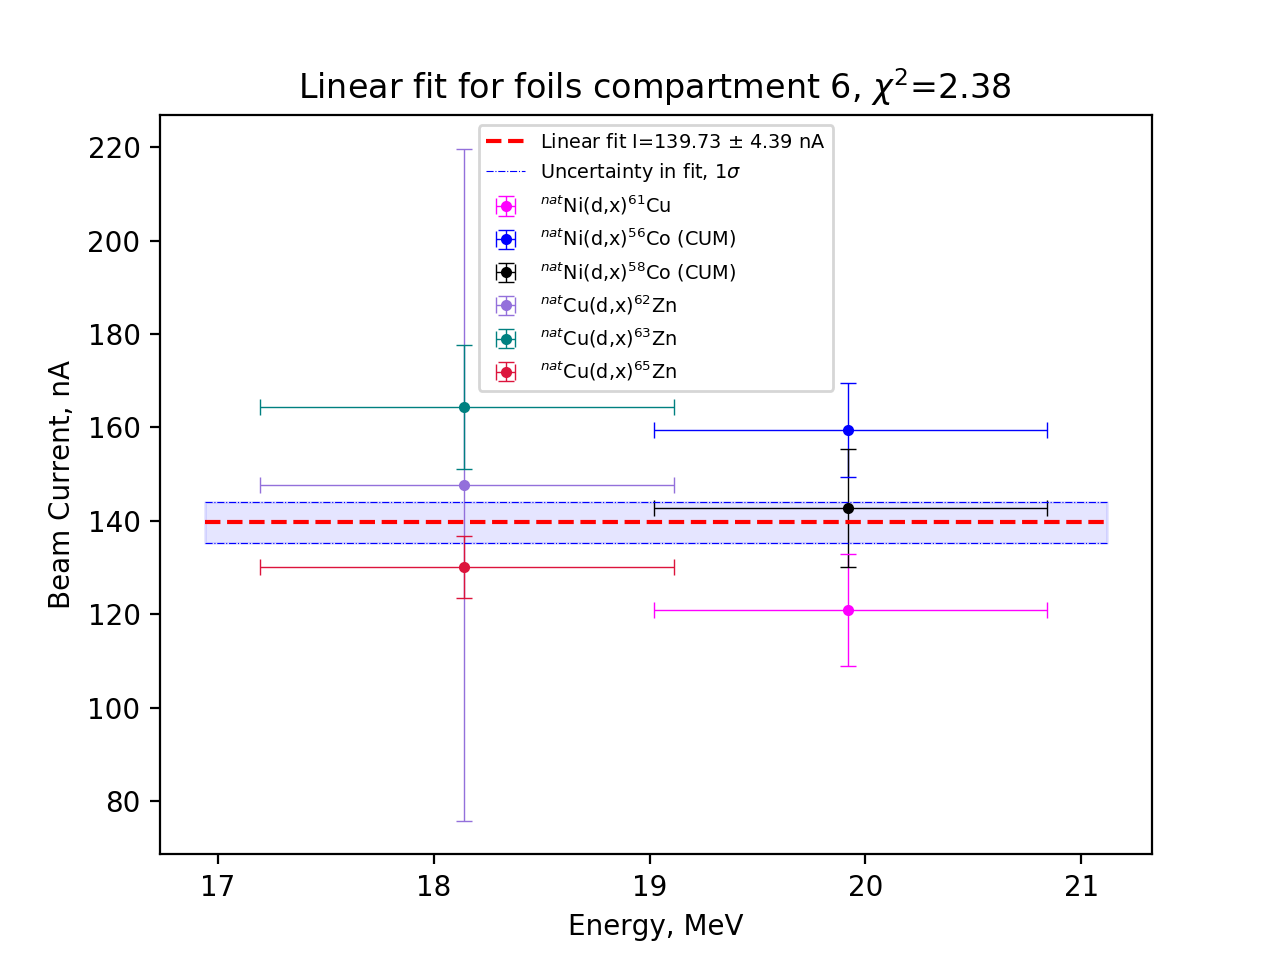
\includegraphics{Analysis/Compartment_6.png}
    \caption{The estimated (uncertainty weighted) beamcurrent over compartment 6. }
    \label{fig:BC_comp6}
\end{figure}

Figure \ref{fig:varmin_beamcurrent} shows the beam current before and after variance minimization, and the weighted average beam currents are listed in table \ref{tab:weighted_BC} estimated before and after the variance minimization. After variance minimization, the beam current estimated in each compartment (stabled lines) were similar, and meanwhile the weighted $\chi^2$ was about the same in compartment 6, it has improved in compartment 3 and very visible in compartment 9. In general the points are also more aligned. 

\begin{figure}%
    \centering
    \subfloat[]{{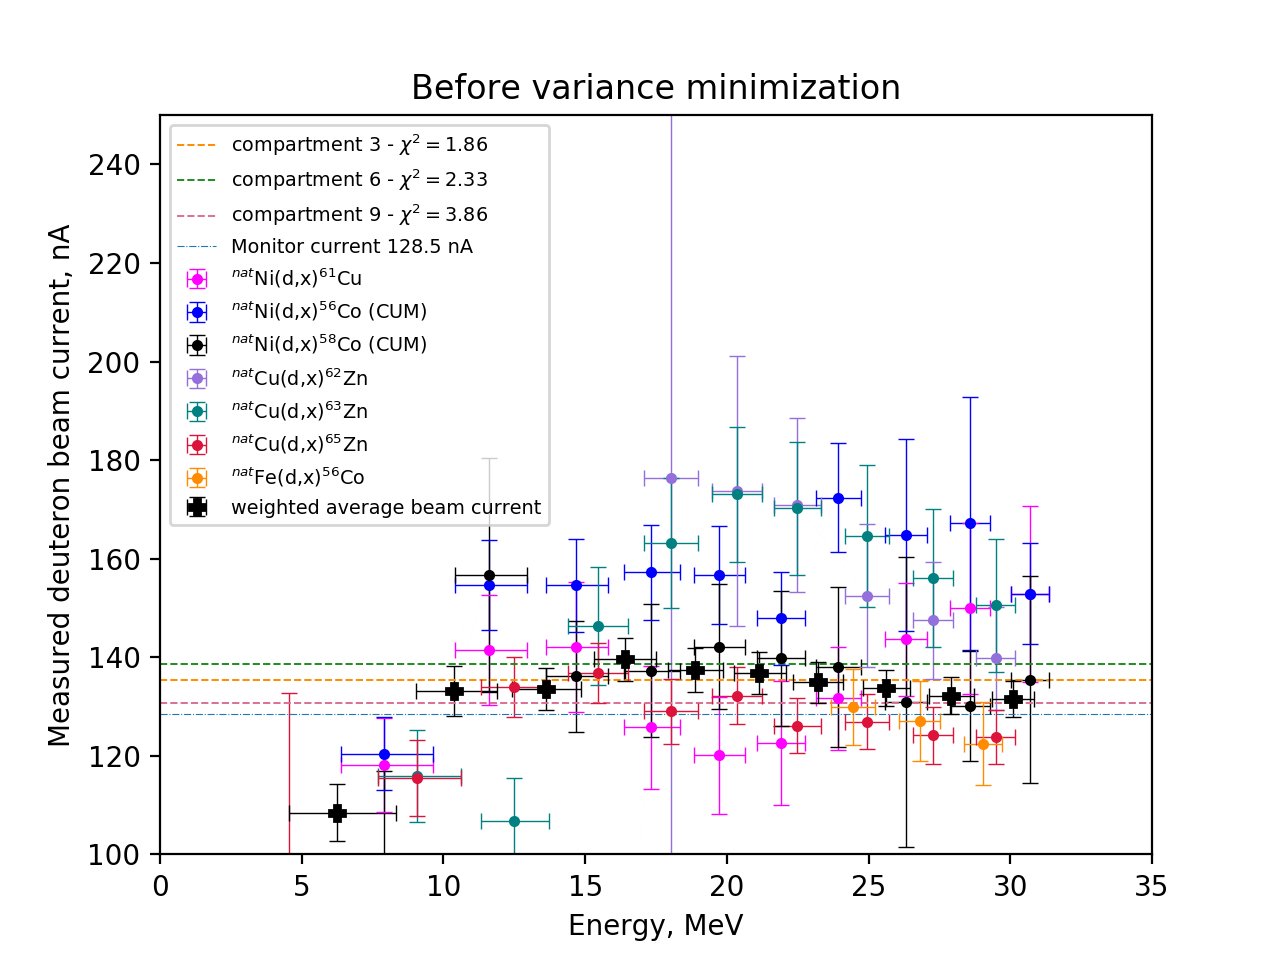
\includegraphics[width=11cm]{Analysis/beamcurrent_B_0_D_0.png} }}\hfill
    \subfloat[A 2\% increase in beam current and a 4.25\% increase in areal density gave the overall most consistent beam current, with reasonable values for the weighted . ]{{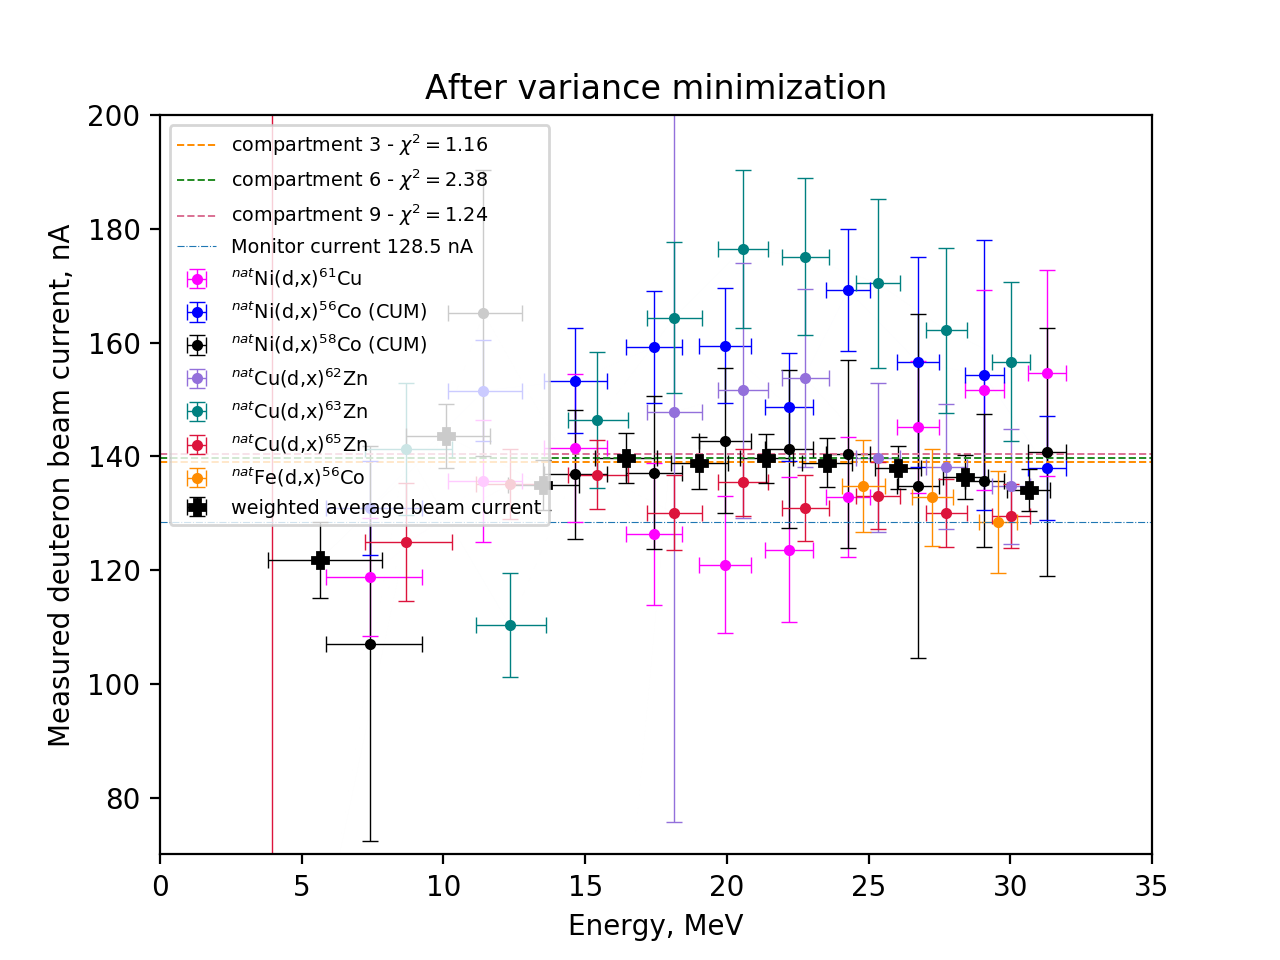
\includegraphics[width=11cm]{Analysis/beamcurrent_B_+2_D_+4,25.png} }}%
    \caption{Beam current before and after variance minimization.  }%
    \label{fig:varmin_beamcurrent}%
\end{figure}


\begin{table}[]
    \centering
        \caption{The weighted average beam current before and after variance minimization in each compartment. The beam current on the 88-Inch Cyclotron beam integrator was 128.5 nA. }
    %\footnotesize
    \begin{tabular}{c|c c c c c c c c c c}
        & \makecell{c_{10}} & \makecell{c_{09}} & \makecell{c_{08}} & \makecell{c_{07}} & \makecell{c_{06}} & \makecell{c_{05}} & \makecell{c_{04}} & \makecell{c_{03}} & \makecell{c_{02}} & \makecell{c_{01}} \\ 
        \hline
         \makecell{Before} & \makecell{131.56_{\pm 3.64}} & \makecell{132.23_{\pm 3.74}} & \makecell{133.81_{\pm3.64 }} & \makecell{134.89_{\pm 4.21 }} & \makecell{136.85_{\pm 4.21}} & \makecell{137.40 _{\pm 4.53}} & \makecell{139.55_{\pm 4.37}} & \makecell{133.60_{\pm 4.27}} & \makecell{133.16_{\pm 5.04}} & \makecell{108.49_{\pm 5.80}}  \\        
         %\makecell{Before} & \makecell{131.56 \pm 3.64} & \makecell{132.23 \pm 3.74} & \makecell{133.81\pm3.64 } & \makecell{134.89\pm 4.21 } & \makecell{136.85_{\pm 4.21}} & \makecell{137.40 \pm 4.53} & \makecell{139.55 \pm 4.37} & \makecell{133.60 \pm 4.27} & \makecell{133.16 \pm 5.04} & \makecell{108.49 \pm 5.80}  \\
         \makecell{After} & \\
    \end{tabular}
    \label{tab:my_label}
\end{table}


\begin{table}[]
    \centering
        \caption{The weighted average beam current before and after variance minimization in each compartment. The beam current on the 88-Inch Cyclotron beam integrator was 128.5 nA.}
    %\footnotesize
    \begin{tabular}{c |c c}
        \hline 
       Compartment & \makecell{Before} & \makecell{After}\\ 
        \hline 
        \makecell{01} & \makecell{131.56 \pm 3.64} & \makecell{134.08 \pm 3.70}  \\ 
        \makecell{02} & \makecell{132.23 \pm 3.74} & \makecell{136.42 \pm 3.83} \\ 
        \makecell{03} & \makecell{133.81 \pm 3.64 } & \makecell{138.02 \pm 3.75} \\ 
        \makecell{04} & \makecell{134.89 \pm 4.21 } &  \makecell{138.88 \pm 4.31}\\ 
        \makecell{05} &\makecell{136.85 \pm 4.21} & \makecell{139.67 \pm 4.29} \\
        \makecell{06} &\makecell{137.40 \pm 4.53} & \makecell{138.85 \pm 4.58} \\
        \makecell{07} &\makecell{139.55 \pm 4.37} & \makecell{139.77 \pm 4.37} \\
        \makecell{08} &\makecell{133.60 \pm 4.27} & \makecell{134.96 \pm 4.32}\\
        \makecell{09} &\makecell{133.16 \pm 5.04} & \makecell{143.59 \pm 5.67} \\
        \makecell{10} &\makecell{108.49 \pm 5.80} & \makecell{121.75 \pm 6.65} \\
    
         %\makecell{Before} & \makecell{131.56 \pm 3.64} & \makecell{132.23 \pm 3.74} & \makecell{133.81\pm3.64 } & \makecell{134.89\pm 4.21 } & \makecell{136.85_{\pm 4.21}} & \makecell{137.40 \pm 4.53} & \makecell{139.55 \pm 4.37} & \makecell{133.60 \pm 4.27} & \makecell{133.16 \pm 5.04} & \makecell{108.49 \pm 5.80}  \\
         %\makecell{After} & \\
    \end{tabular}
    \label{tab:weighted_BC}
\end{table}
\end{comment}
For cross section calculations, equation \ref{eq:CrossSection_general} is used, with the estimated weighted average beam current. Figure \ref{fig:monitor_BC+CS} shows the estimated cross sections for the monitor reactions, using the weighted average beam current over all monitor foils. The recommended monitor cross section data for the monitor reactions are also plotted, which was used in the cross section calculation.  



\begin{figure}%
    \centering
    \subfloat[]{{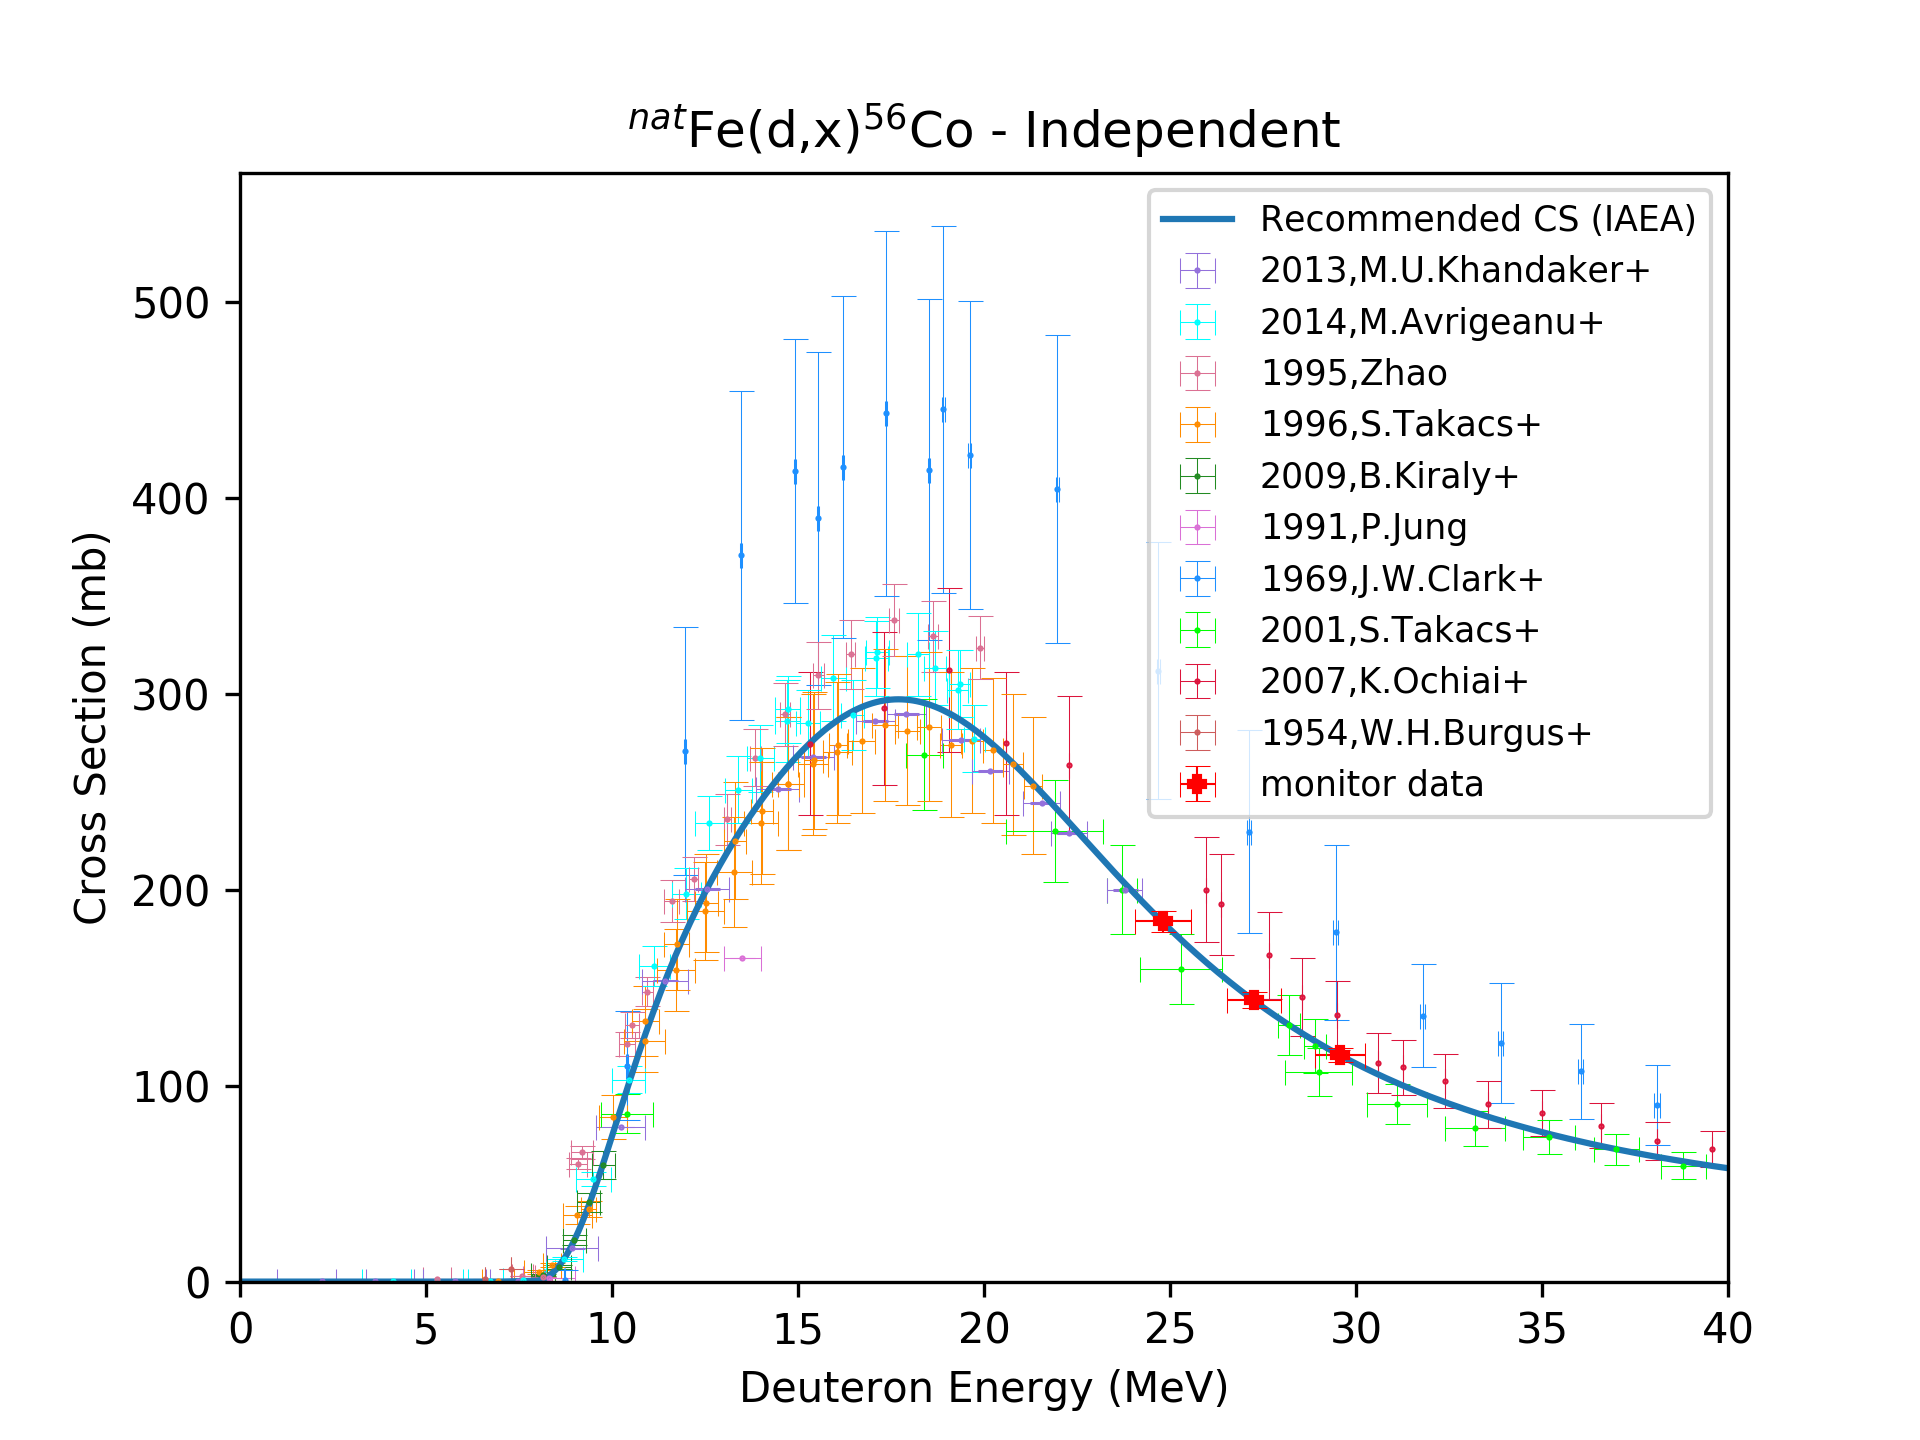
\includegraphics[width=7.5cm]{Analysis/Fe_56Co.png} }}%
    \quad
    \subfloat[]{{\includegraphics[width=7.5cm]{Analysis/Ni_61Cu.png} }}%
    \subfloat[]{{\includegraphics[width=7.5cm]{Analysis/Ni_56Co.png} }}%
    \quad
    \subfloat[]{{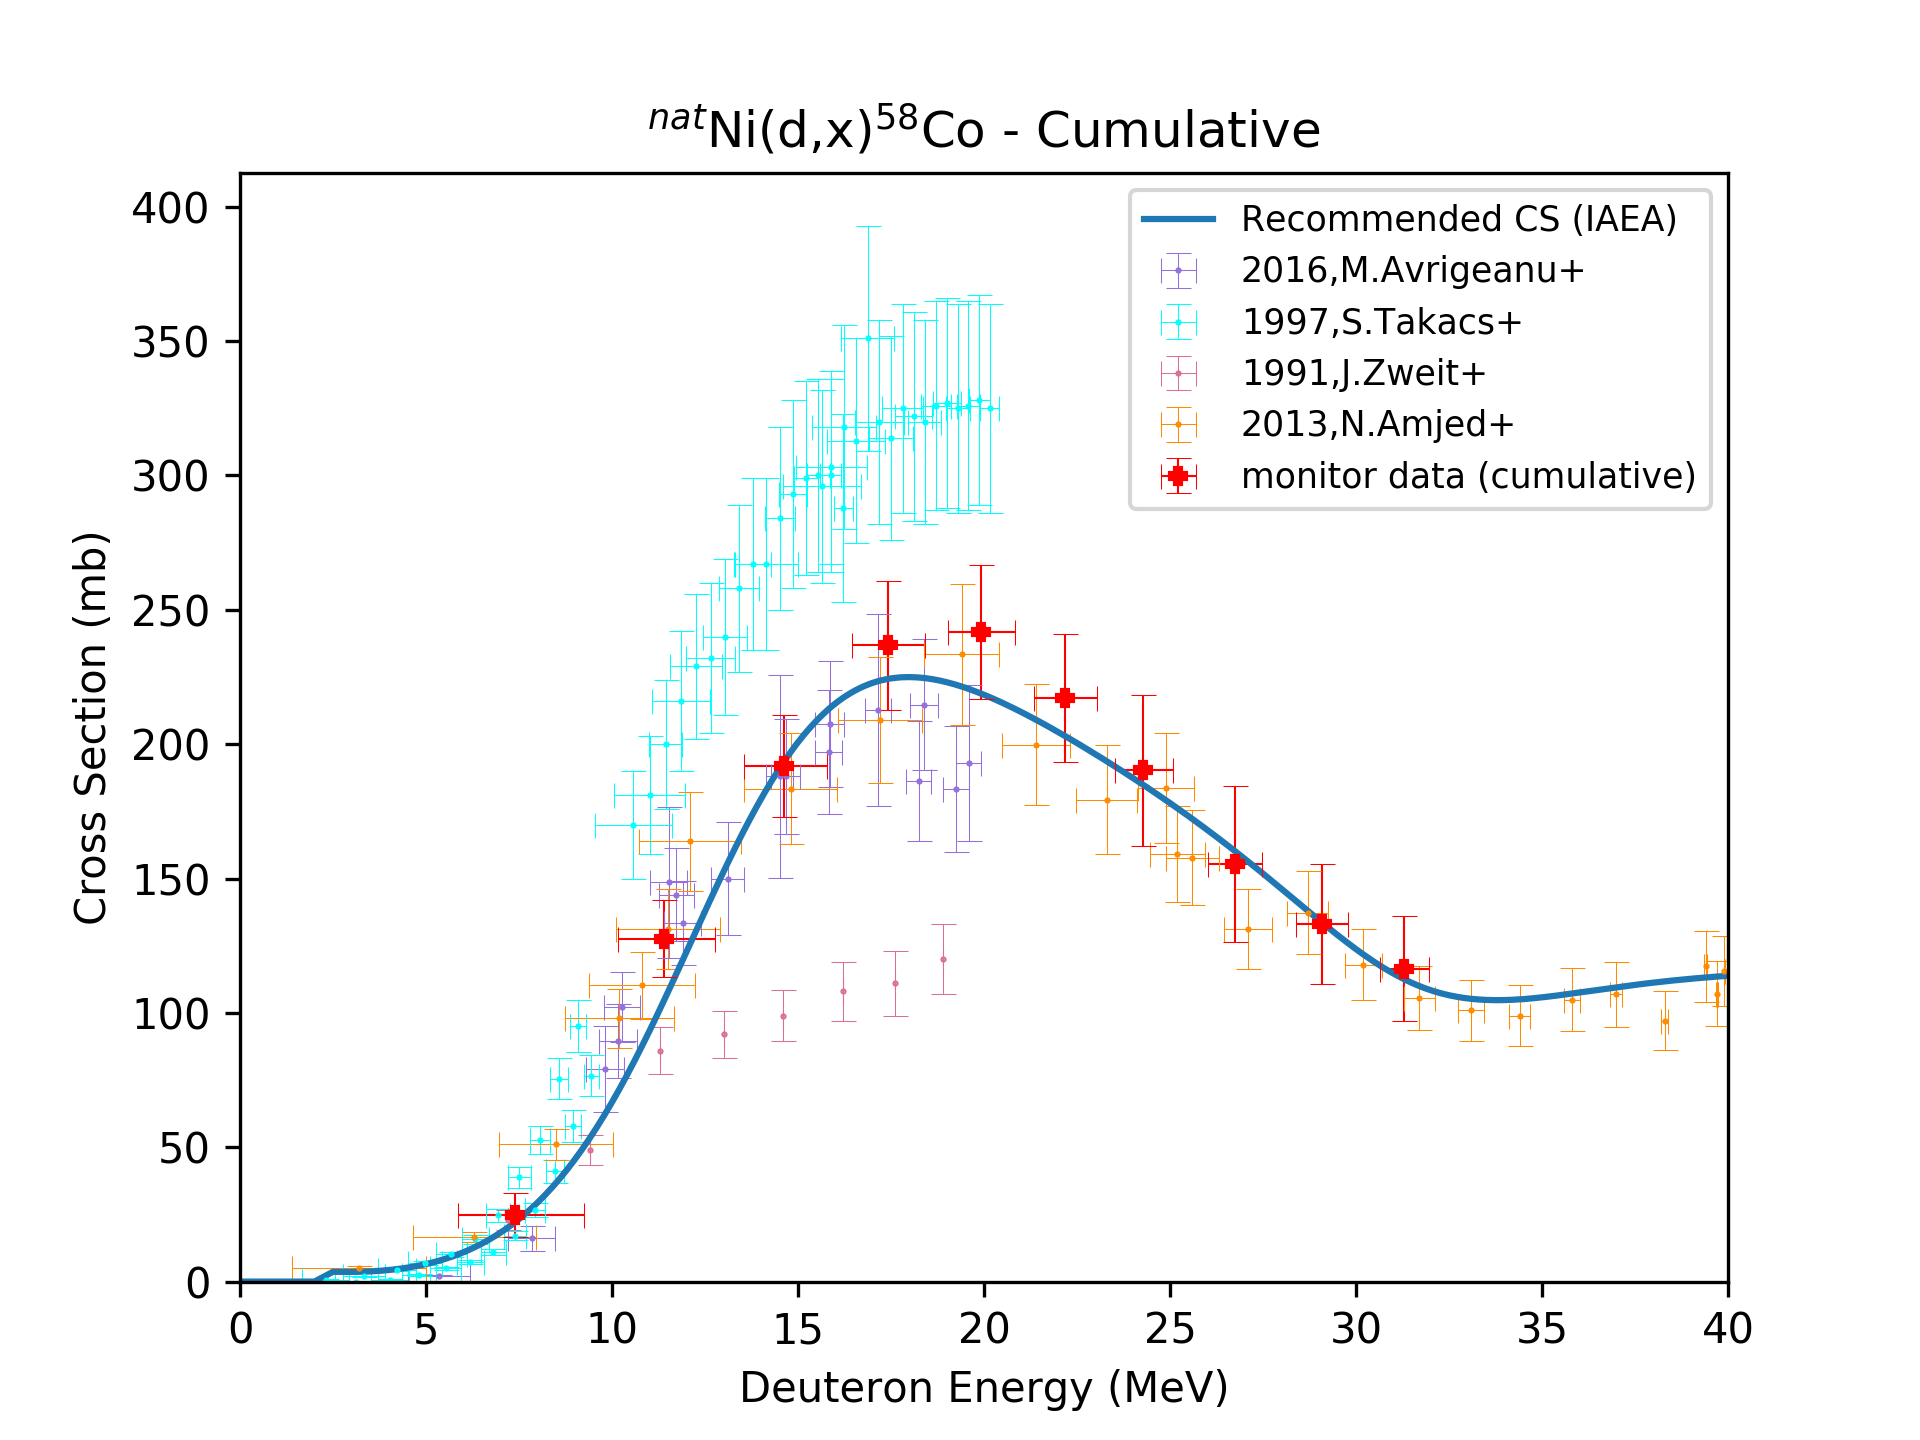
\includegraphics[width=7.5cm]{Analysis/Ni_58Co.png} }}%
    \quad
    \subfloat[caption]{{\includegraphics[width=7.5cm]{Analysis/Cu_62Zn.png} }}%
    \quad
    \subfloat[]{{\includegraphics[width=7.5cm]{Analysis/Cu_63Zn.png} }}%
    \quad
    \subfloat[]{{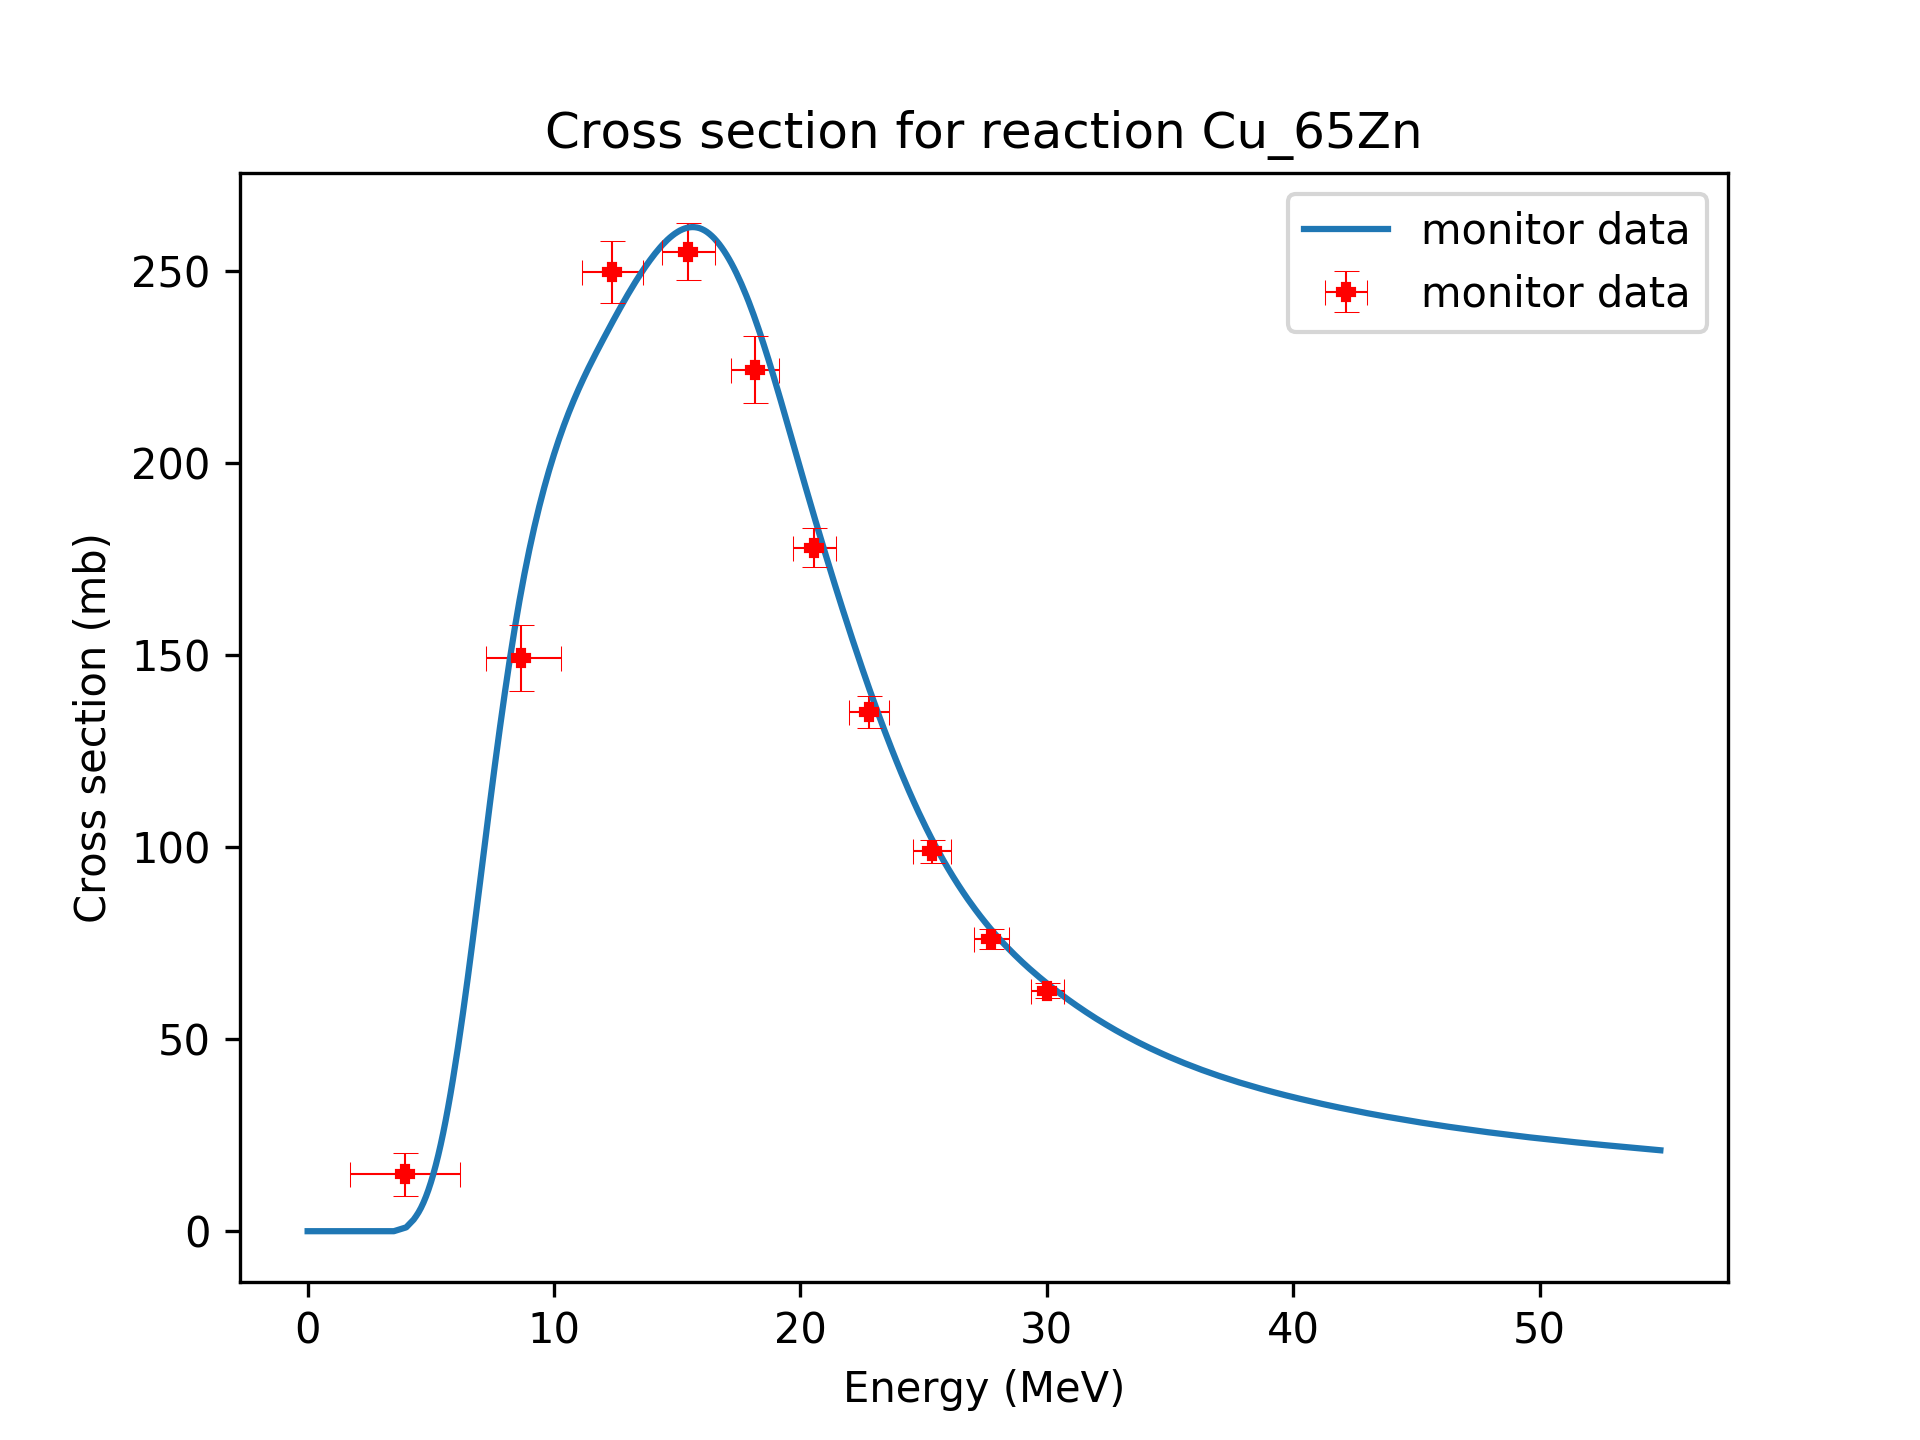
\includegraphics[width=7.5cm]{Analysis/Cu_65Zn.png} }}%
    \quad
    \caption{Figure shows the estimation of monitor cross section using the estimated weighted average beam current for each reaction (not the total). It is compared along with the recommended (IAEA) monitor data, and other experimental data  }%
    \label{fig:monitor_BC+CS}%
\end{figure}

\section{Cross section measurements} 
With all variables for cross sections, cross sections can be calculated using equation \ref{eq:CrossSection_generall}. Since the energy was a flux-weighted average beam energy, the value that is provided as cross section is a flux-averaged cross section. An accurate measure of the cross section as a function of deuteron energy was possible, as the thin foils provides smaller average beam energy intervals, and it makes it possible to have more measurements if thick foils are replaced with several thinner (one single foil represents a single measurement). \textcolor{red}{in theory: Thin foils also produce minimal amounts of radioactivity, thus the deadtime of the detector and the dose to humans is low.}% For charged particles, the stopping power is inversely proportional to their energy\footnote{Andrew S. Voyles, Lee A. Bernstein, Eva R. Birnbaum, Jonathan W. Engle, Stephen A.
%Graves, Toshihiko Kawano, Amanda M. Lewis, and Francois M. Nortier. Excitation functions
%for (p,x) reactions of niobium in the energy range of Ep = 40–90 MeV. Nuclear Instruments
%and Methods in Physics Research Section B: Beam Interactions with Materials and Atoms,
%429:53–74, aug 2018.}, and therefor the energy degradation in thicker foils will be large. For thin targets, we can however assume that the stopping power $dE/dx\simeq 0$, and the cross section can be replaced with a differential (normalized) cross section 
%
%\begin{equation}
%    \sigma(E) = \frac{\int \sigma(E) \frac{d\phi}{dE}dE}{\int \frac{d\phi}{dE}dE}
%\end{equation}

%The energy-limits in the integral can be minimized and the error in the energy for charged particles will be small. \\

\textcolor{blue}{Thin foils decreases the energy width, making a more precise measurement dependent on energy. However the reported cross sections are flux-averaged over the energy distribution subtended by each foil. } 

The cross sections are reported as independent if there is nothing decaying into it (beta feeding or from isomer transition), which means that the first observed element in a decay chain is reported as cumulative unless it is the first possible element (which are the nuclei with one more proton more than the target nuclei, which for this experiment is Platinum (from Ir), Zink (from Cu), Copper (from Ni) and Cobalt (from Fe). If there is feeding, and the half life is much shorter or much longer than the specific nuclei, can choose appropirate timewindow and report as independent, when we know that the feeding has either died out or is very low! 

If possible with feeding: added together to get cumulative or subtracted giving independent. Multiplying by branching ratio. 

The measured cross sections in this work was compared to previous experimental data, along with reaction modelling codes TALYS\foonote{https://sci-hub.tw/https://doi.org/10.1016/j.nds.2012.11.002}, TENDL, ALICE20 and CoH. \\

\noindent 
\textcolor{blue}{from talys cite, p. 2844: Software for the analysis and prediction of nuclear reactions that involve neutrons, photons, protons, deuterons, tritons, $^3$He and alphaparticles, in the 1keV-200 MeV energy range and for target radionuclides of mass 5 and heavier. A suite of nuclear reaction models has been implemented in one single code system. This enables to evaluate nuclear reactions from the unresolved resonance range up to intermediate energies. Can have many different outputs we are interested in exclusive channnel cross sections, energy and double differential spectra p. 2845. 

Optical model calculations performed first, }

Talys takes in projectile, target element (specific isotope or all stable target isotopes), energy array with desired spacing and upper limit energy. 

\textcolor{blue}{from Andrew mail: Each code was ran on default parameters (no changes to nuclear structure or the modeling of the reaction physics). Adjusting allows to tune the code to match experimental data, but this is of limited value as the parameters you settle on to match one product nucleus causes most of the others to get even worse - i.e., its a local optimization, not improving the code globally.  We run our codes for papers on defaults, as 1) that's how 99\% of users do so, and 2) it reveals how good each code's predictive power is. 

For COH: To get both 191Ir and 193Ir to run, we had to adjust the parameter "tweakSD", which adjusts the effective single-particle state density for a particular particle emission channel.  In the end, we ran with tweakSD=0.25  for both outgoing alphas and neutrons  (protons were unaffected).  In other words, we set the single-particle state density for outgoing alphas and neutrons [(d,xa) and (d,xn) reactions]  to be 25\% of what they normally are, which is a HUGE change.} 


\textcolor{blue}{from talys cite p. 2843-2844: TENDL is developed from talys (TALYS evaluated Nuclear data Library).  This
library consists of a complete set of nuclear reaction data
for incident neutrons, photons, protons, deuterons, tritons, Helium-3 and alpha particles, from 10$^−5$ eV up to 200 MeV, for all 2430 isotopes from 6Li to 281Ds that are either stable of have a half-life longer than 1 second.
All data are completely and consistently evaluated using a software system consisting of the TALYS nuclear reaction code, and other software to handle resonance data, experimental data, data from existing evaluations,
and to provide the final ENDF-6 formatting, including
covariance information. The result is a nuclear data library with mutually consistent reaction information for
all isotopes and a quality that increases with yearly updates.  To produce this library, TALYS input parameters are
adjusted for many nuclides so that calculated cross sections agree with experimental data, while for important
nuclides experimental or evaluated data are directly included. Also feedback from integral measurements is
processed into the data libraries. For nuclides for which
(almost) no experimental data exists, default TALYS
calculations based on global models and parameters are
used.}


Dont understand this part..... 


\chapter{Results}




\begin{figure}%
    \centering
    \subfloat[A cumulative measurement of $^{188}$Ir isomer and ground state, and beta-feeding feeding from $^{188}$Pt (100\%)]{{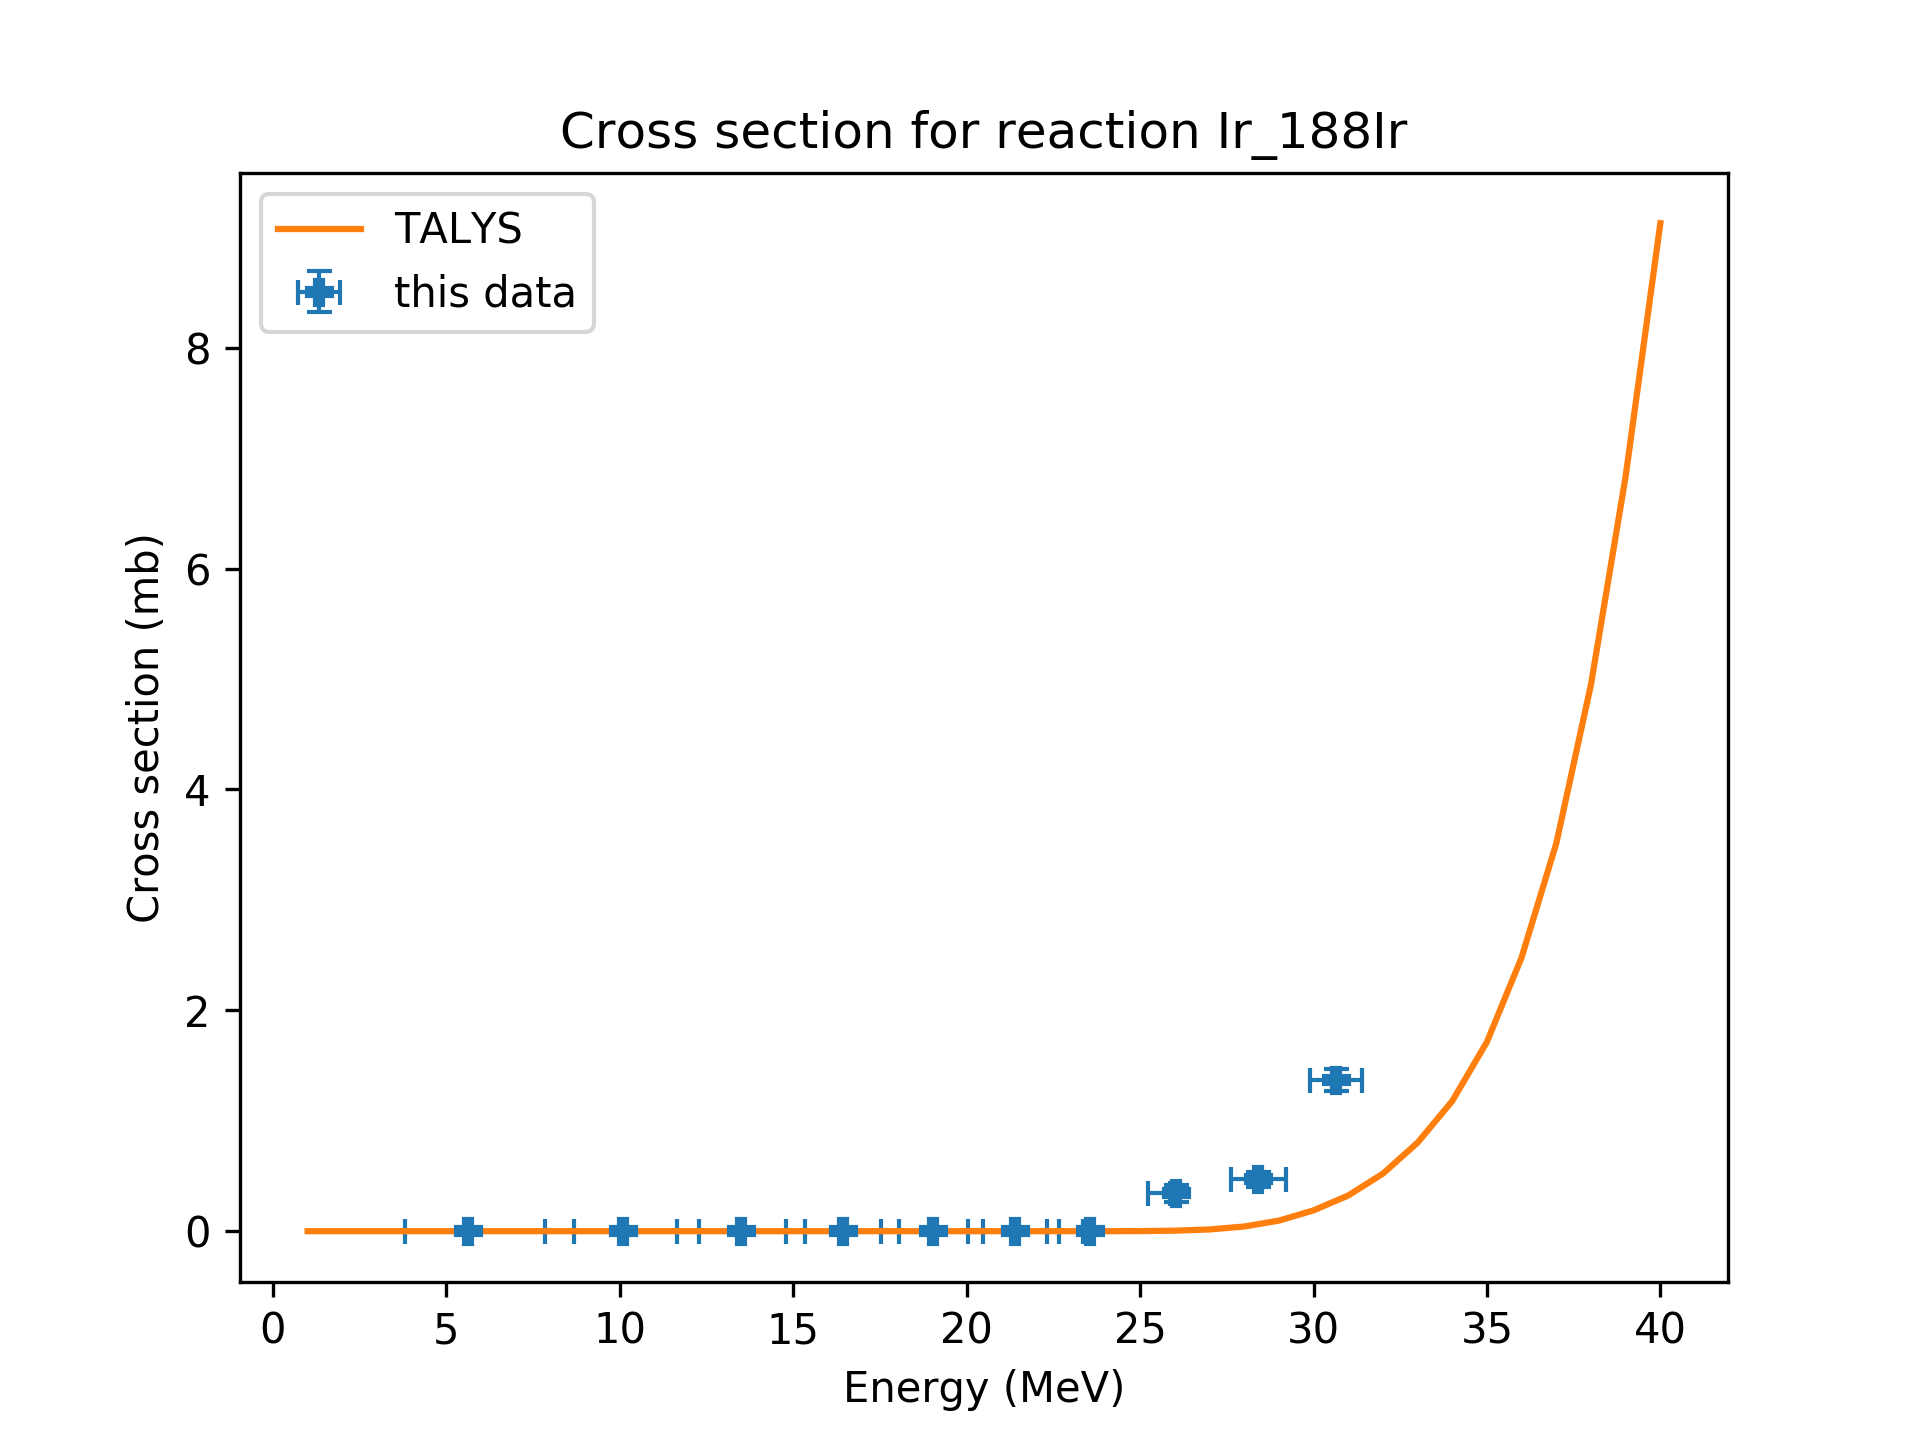
\includegraphics[width=8cm]{Results/Ir_188Ir.png} }}%
    \quad
    \subfloat[An independent measurement of the cumulative cross section for $^{188}$Ir isomer and ground state, with subtraction of the feeding-weighted percentage of $^{188}$Pt from the cumulative cross section. ]{{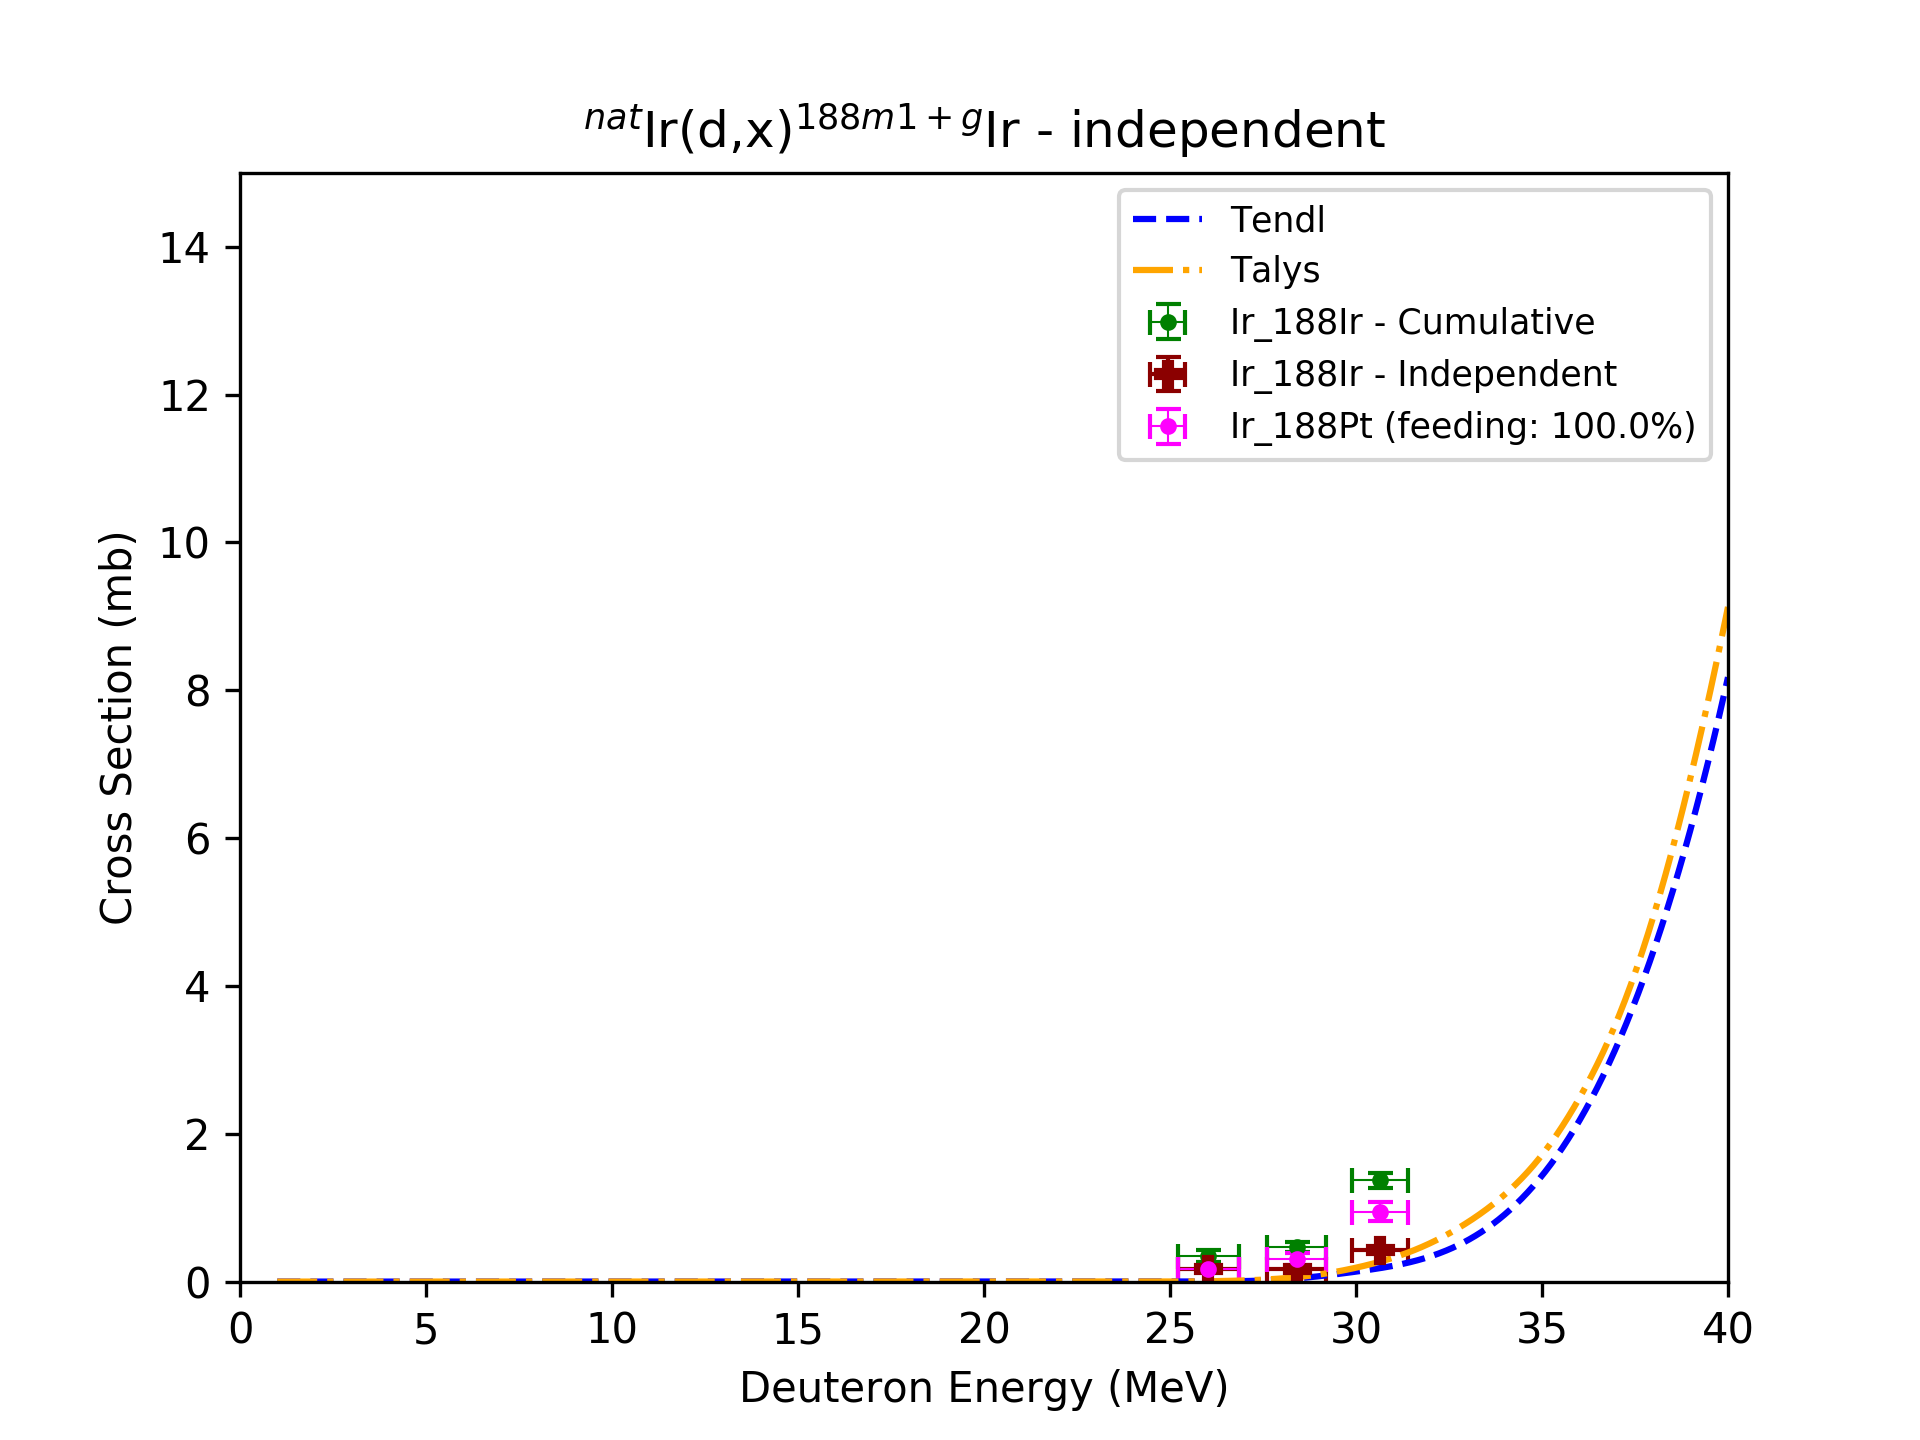
\includegraphics[width=8cm]{Results/Ir_188Ir_subtracted.png} }}%
    \quad
    \subfloat[A cumulative measurement of $^{189}$Ir isomers and ground state, and beta-feeding from $^{189}$Pt (100\%).]{{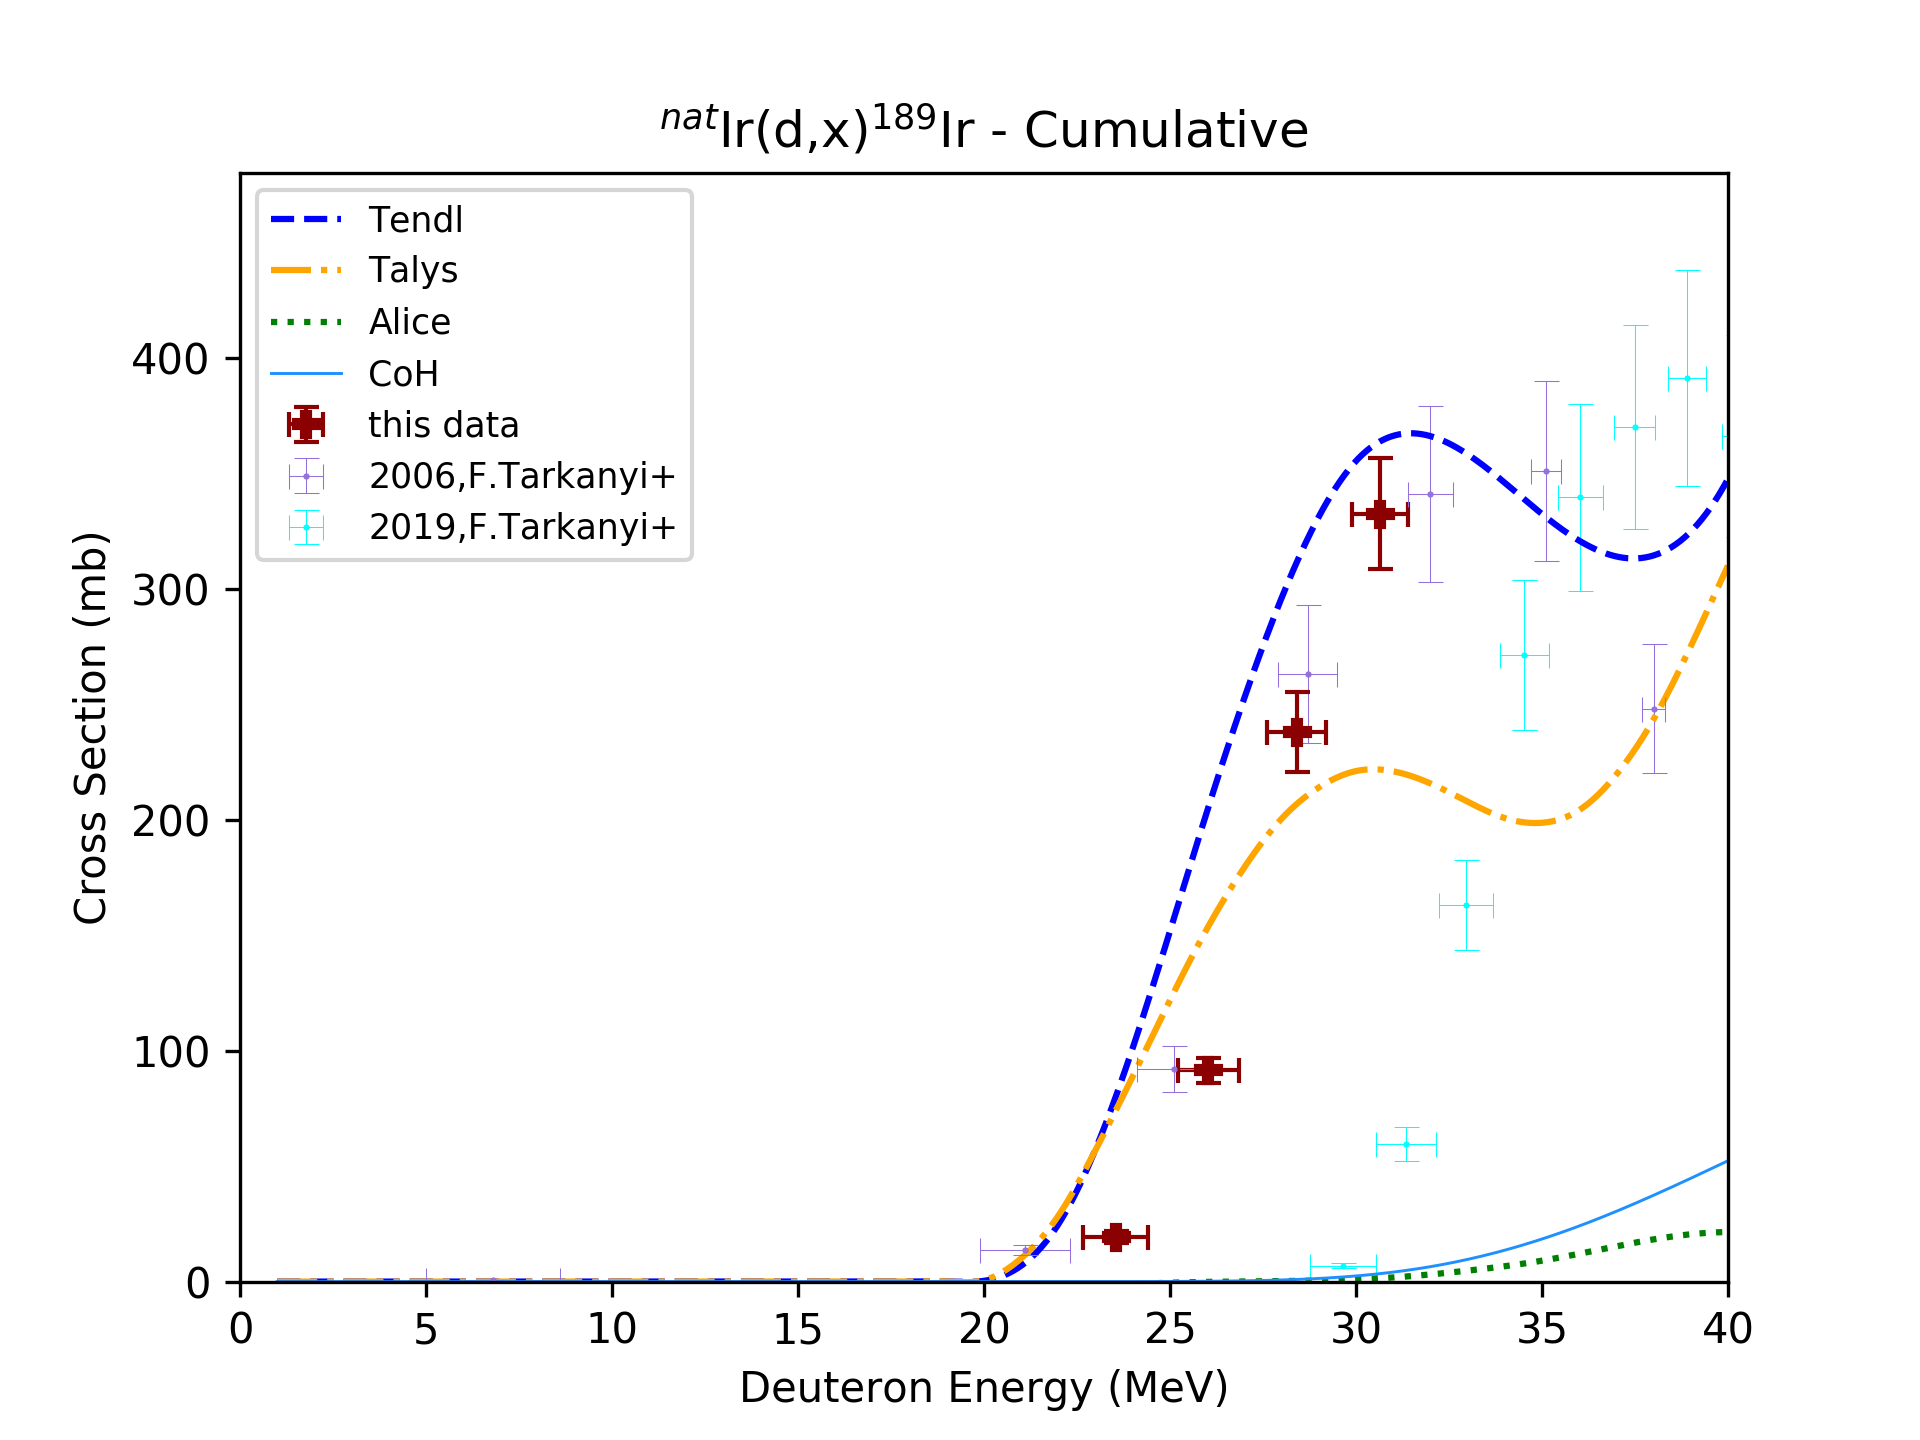
\includegraphics[width=8cm]{Results/Ir_189Ir.png} }}%
    \quad
    \subfloat[A cumulative measurement of $^{190m1+m2+g}$ (m1: 100\%, m2: 8.60\%). ]{{\includegraphics[width=8cm]{Results/Ir_190Ir.png} }}%
    \quad
    \subfloat[An independent measurement of the cumulative cross section for $^{190m1+g}$Ir, with subtraction of the feeding weighted percentage of $^{190m2}$Ir. ]{{\includegraphics[width=8cm]{Results/Ir_190Ir_subtracted.png} }}%
    \quad
      \caption{Excitation functions for $^{188m1+g}$Ir (independent and cumulative) and $^{189}$Ir (cumulative)  }%
    \label{fig:cross-sections_188,189Ir}%
\end{figure}   

\begin{figure}%
    \centering
    \subfloat[An independent measurement of $^{190m2}$Ir. ]{{\includegraphics[width=8cm]{Results/Ir_190m2Ir.png} }}%
    \quad
    \subfloat[An independent measurement of the cumulative cross section for $^{192}$Ir isomers (m1: 99.98\%, m2: 100\%)]{{\includegraphics[width=8cm]{Results/Ir_192Ir.png} }}%
    \quad
    \subfloat[An independent measurement of the cumulative cross section for $^{194m1+g}$ (m1:100\%)]{{\includegraphics[width=8cm]{Results/Ir_194Ir.png} }}%
    \quad
    \subfloat[An independent measurement of $^{194m2}$Ir. ]{{\includegraphics[width=8cm]{Results/Ir_194m2Ir.png} }}%
    \caption{Excitation functions for $^{190m1+m2+g}$Ir (cumulative), $^{190m1+g}$Ir (cumulative), $^{190m2}$Ir (independent), $^{194m1+g}$Ir (cumulative) and $^{194m2}$Ir (independent)  }%
    \label{fig:cross-sections_190,194Ir}%
\end{figure}







\begin{figure}%
    \centering
    \subfloat[An independent measurement of $^{188}$Pt. ]{{\includegraphics[width=8cm]{Results/Ir_188Pt.png} }}%
    \quad
    \subfloat[An independent measurement of $^{189}$Pt. ]{{\includegraphics[width=8cm]{Results/Ir_189Pt.png} }}%
    \quad
    \subfloat[An independent measurement of $^{191}$Pt. ]{{\includegraphics[width=8cm]{Results/Ir_191Pt.png} }}%
    \quad
    \subfloat[An independent measurement of $^{193m}$Pt.]{{\includegraphics[width=8cm]{Results/Ir_193mPt.png} }}%
    \quad 
    \caption{Excitation functions for Platinum radionuclides }%
    \label{fig:cross-sections_Pt}%
\end{figure}

\begin{figure}%
    \centering
    \subfloat[A cumulative measurement of $^{48}$V. ]{{\includegraphics[width=8cm]{Results/Fe_48V.png} }}%
    \quad
    \subfloat[A cumulative measurement of $^{51}$Cr. ]{{\includegraphics[width=8cm]{Results/Fe_51Cr.png} }}%
    \quad
    \subfloat[A cumulative measurement of $^{52}$Mn isomer (IT: 98.25\%) and groundstate. ]{{\includegraphics[width=8cm]{Results/Fe_52Mn.png} }}%
    \quad
    \subfloat[An independent measurement of $^{54}$Mn.]{{\includegraphics[width=8cm]{Results/Fe_54Mn.png} }}%
    \quad
    \subfloat[A cumulative measurement of $^{53}$Fe. ]{{\includegraphics[width=8cm]{Results/Fe_53Fe.png} }}%
    \quad
      \caption{Excitation functions for $^{48}$V, $^{51}$Cr, $^{52}$Mn, $^{54}$Mn, $^{53}$Fe produced from iron.  }%
    \label{fig:cross-sections_188,189Ir}%
\end{figure} 

\begin{figure}%
    \centering
    \subfloat[An independent measurement of $^{59}$Fe. ]{{\includegraphics[width=8cm]{Results/Fe_59Fe.png} }}%
    \quad
    \subfloat[An independent measurement of $^{55}$Co. ]{{\includegraphics[width=8cm]{Results/Fe_55Co.png} }}%
    \quad
    \subfloat[An independent measurement of $^{57}$Co. ]{{\includegraphics[width=8cm]{Results/Fe_57Co.png} }}%
    \quad
    \subfloat[An independent measurement of $^{58}$Co. ]{{\includegraphics[width=8cm]{Results/Fe_58Co.png} }}%
    \quad
      \caption{Excitation functions for $^{59}$Fe, $^{55}$Co, $^{57}$Co, $^{58}$Co produced from iron.  }%
    \label{fig:cross-sections_188,189Ir}%
\end{figure} 

\begin{figure}%
    \centering
    \subfloat[A cumulative measurement of $^{59}$Fe]{{\includegraphics[width=8cm]{Results/Cu_59Fe.png} }}%
    \quad
    \subfloat[A cumulative measurement of $^{60}$Co of isomer (IT:99.75\%) and groundstate. ]{{\includegraphics[width=8cm]{Results/Cu_60Co.png} }}%
    \quad
    \subfloat[A cumulative measurement of $^{61}$Co. ]{{\includegraphics[width=8cm]{Results/Cu_61Co.png} }}%
    \quad
    \subfloat[An independent measurement of $^{65}$Ni.]{{\includegraphics[width=8cm]{Results/Cu_65Ni.png} }}%
    \quad
    \subfloat[A cumulative measurement of $^{62}$Cu.]{{\includegraphics[width=8cm]{Results/Cu_61Cu.png} }}%
    \quad
    \subfloat[An independent measurement of $^{64}$Cu.]{{\includegraphics[width=8cm]{Results/Cu_64Cu.png} }}%
    \quad
      \caption{Excitation functions for $^{59}$Fe, $^{55}$Co, $^{57}$Co, $^{58}$Co produced from iron.  }%
    \label{fig:cross-sections_188,189Ir}%
\end{figure} 




\begin{comment}
\begin{table}[]
    \centering
    \footnotesize
    \begin{tabular}{c c c c c c c c c c c} 
        \hline
       \makecell{E_d (MeV)}  &  \makecell{30.65_{-0.75}^{+0.76}} & \makecell{28.40_{-0.79}^{+0.80}} & \makecell{26.03_{-0.82}^{+0.82}} & \makecell{23.54_{-0.87}^{+0.88}} & \makecell{21.38_{-0.92}^{+0.94}} & \makecell{19.03_{-0.99}^{+1.00}} & \makecell{16.43_{-1.08}^{+1.11}} & \makecell{13.51_{-1.22}^{+1.28}} & \makecell{10.09_{-1.41}^{+1.55}} & \makecell{5.63_{-1.83}^{+2.21}}   \\
       \hline
       
       \makecell{$^{188}$Ir} & \makecell{} & \makecell{} & \makecell{} &  \makecell{} &  \makecell{} &  \makecell{} &  \makecell{} &  \makecell{} &  \makecell{} &  \makecell{} \\
       \makecell{$^{193m}$Pt} & \makecell{48.11 \pm 6.33} & \makecell{} & \makecell{} &  \makecell{} &  \makecell{} &  \makecell{} &  \makecell{} &  \makecell{} &  \makecell{} &  \makecell{} \\       
       
    \end{tabular}
    \caption{Iridium cross sections. }
    \label{tab:my_label}
\end{table}



\newpage
\pagestyle{empty}
\begingroup
\setlength{\tabcolsep}{10pt} % Default value: 6pt
\renewcommand{\arraystretch}{1.2} % Default value: 1
%\begin{landscape}
%\begin{table}[]
\begin{sidewaystable}
    \centering
    \small
    \begin{tabular}{c c c c c c c c c c c} 
        \hline
        
        & \multicolumn{8}{c}{ Production cross section (mb) for $^\text{mat}$Ir(d,x) radionuclides}\\
        \hline
        %& \multicolumn{10}{c}{\hline} \\
       \makecell{$E_d$ (MeV)}  &  \makecell{30.65_{-0.75}^{+0.76}} & \makecell{28.40_{-0.79}^{+0.80}} & \makecell{26.03_{-0.82}^{+0.82}} & \makecell{23.54_{-0.87}^{+0.88}} & \makecell{21.38_{-0.92}^{+0.94}} & \makecell{19.03_{-0.99}^{+1.00}} & \makecell{16.43_{-1.08}^{+1.11}} & \makecell{13.51_{-1.22}^{+1.28}} & \makecell{10.09_{-1.41}^{+1.55}} & \makecell{5.63_{-1.83}^{+2.21}}   \\
       \hline
       \makecell{$^{188m1+g}$Ir$_\text{cum}$} & \makecell{1.36 \pm 0.10} & \makecell{0.47 \pm 0.07} & \makecell{0.34 \pm 0.08} & \makecell{-} & \makecell{-} & \makecell{-} & \makecell{-} & \makecell{-} & \makecell{-} & \makecell{-} \\
       \makecell{$^{188m1+g}$Ir$_\text{ind}$} & \makecell{0.42 \pm 0.03} & \makecell{0.17 \pm 0.02} & \makecell{0.17 \pm 0.03} & \makecell{-} & \makecell{-} & \makecell{-} & \makecell{-} & \makecell{-} & \makecell{-} & \makecell{-} \\
       \makecell{$^{189}$Ir$_\text{cum}$} & \makecell{332.48 \pm 24.2} & \makecell{237.84 \pm 17.44} & \makecell{91.49 \pm 5.47} & \makecell{19.23 \pm 2.65} & \makecell{-} &
       \makecell{-} & \makecell{-} & \makecell{-} & \makecell{-} & \makecell{-} \\
       \makecell{$^{190m1+g}$Ir$_\text{cum}$} & \makecell{86.65\pm 2.89} & \makecell{62.80 \pm 2.14} & \makecell{44.26 \pm 1.46} & \makecell{27.29 \pm 1.02} & \makecell{18.73 \pm 0.71} &
       \makecell{14.02 \pm 0.55} & \makecell{12.40 \pm 0.51} & \makecell{8.26 \pm 0.43} & \makecell{-} & \makecell{-} \\
       \makecell{$^{190m1+g}$Ir$_\text{ind}$} & \makecell{} & \makecell{} & \makecell{} & \makecell{} & \makecell{} \\
       \makecell{} & \makecell{} & \makecell{} & \makecell{} & \makecell{} \\
       \makecell{$^{190m2}$Ir$_\text{ind}$} & \makecell{8.87 \pm 0.25} & \makecell{5.03 \pm 0.15} & \makecell{2.92 \pm 0.08} & \makecell{1.16 \pm 0.04 } & \makecell{0.45 \ pm 0.01} &
       \makecell{0.16 \pm 0.01} & \makecell{0.06 \pm 0.01} & \makecell{0.03 \pm 0.00} & \makecell{0.02 \pm 0.00} & \makecell{0.02 \pm 0.00} \\
       \makecell{$^{192}$Ir$_\text{cum}$} & \makecell{} & \makecell{} & \makecell{} & \makecell{} & \makecell{} \\
       \makecell{} & \makecell{} & \makecell{} & \makecell{} & \makecell{} \\
       \makecell{$^{194m1+g}$Ir$_\text{ind}$} & \makecell{} & \makecell{} & \makecell{} & \makecell{} & \makecell{} \\
       \makecell{} & \makecell{} & \makecell{} & \makecell{} & \makecell{} \\
       \makecell{$^{194m2}$Ir$_\text{ind}$} & \makecell{} & \makecell{} & \makecell{} & \makecell{} & \makecell{} \\
       \makecell{} & \makecell{} & \makecell{} & \makecell{} & \makecell{} \\
       \makecell{$^{188}$Pt$_\text{ind}$} & \makecell{} & \makecell{} & \makecell{} & \makecell{} & \makecell{} \\
       \makecell{} & \makecell{} & \makecell{} & \makecell{} & \makecell{} \\
       \makecell{$^{189}$Pt$_\text{ind}$} & \makecell{} & \makecell{} & \makecell{} & \makecell{} & \makecell{} \\
       \makecell{} & \makecell{} & \makecell{} & \makecell{} & \makecell{} \\
       \makecell{$^{191}$Pt$_\text{ind}$} & \makecell{} & \makecell{} & \makecell{} & \makecell{} & \makecell{} \\
       \makecell{} & \makecell{} & \makecell{} & \makecell{} & \makecell{} \\
       \makecell{$^{193m}$Pt$_\text{ind}$} & \makecell{} & \makecell{} & \makecell{} & \makecell{} & \makecell{} \\
       \makecell{} & \makecell{} & \makecell{} & \makecell{} & \makecell{} \\
       %\makecell{\makecell{28.40_{-0.79}^{+0.80}}} & \makecell{} & \makecell{} & \makecell{} & \makecell{} \\
       
       
       %\makecell{28.40_{-0.79}^{+0.80}} & \makecell{26.03_{-0.82}^{+0.82}} & \makecell{23.54_{-0.87}^{+0.88}} & \makecell{21.38_{-0.92}^{+0.94}} & \makecell{19.03_{-0.99}^{+1.00}} & \makecell{16.43_{-1.08}^{+1.11}} & \makecell{13.51_{-1.22}^{+1.28}} & \makecell{10.09_{-1.41}^{+1.55}} & \makecell{5.63_{-1.83}^{+2.21}}   \\
       \hline
       
       %\makecell{$^{188}$Ir} & \makecell{} & \makecell{} & \makecell{} &  \makecell{} &  \makecell{} &  \makecell{} &  \makecell{} &  \makecell{} &  \makecell{} &  \makecell{} \\
       %\makecell{$^{193m}$Pt} & \makecell{48.11 \pm 6.33} & \makecell{} & \makecell{} &  \makecell{} &  \makecell{} &  \makecell{} &  \makecell{} &  \makecell{} &  \makecell{} &  \makecell{} \\       
       
    \end{tabular}
    \caption{Platinum production cross sections produced from Iridium}
    \label{tab:my_label}
\end{sidewaystable}
%\end{landscape}
\endgroup
\pagestyle{empty}


\begingroup
\setlength{\tabcolsep}{10pt} % Default value: 6pt
\renewcommand{\arraystretch}{1.5} % Default value: 1
\begin{table}[]
    \centering
    \footnotesize
    \begin{tabular}{c  c c c c c c c }
        \hline
        
        & \multicolumn{4}{c}{ \underline{Production cross section (mb) for iridium radionuclides}}\\
        %\hline
       \makecell{$E_d$ (MeV)}   & \makecell{$^{188}$Ir$_\text{cum}$} & \makecell{$^{189}$Ir$_\text{cum}$} & \makecell{$^{190m1+g}$Ir$_\text{cum}$} & \makecell{$^{192m2}$Ir$_\text{ind}$} & \makecell{$^{192}$Ir$_\text{cum}$ } & \makecell{$^{194m1+g}$Ir$_\text{ind}$} & \makecell{$^{194m2}$Ir$_\text{ind}$} \\
       \hline
       \makecell{30.65_{-0.75}^{+0.76}} & \makecell{0.94 \pm 0.13} & \makecell{486.47 \pm 21.86} & \makecell{597.10 \pm 16.55} & \makecell{48.11 \pm 6.33} & \makecell{1.36 \pm 0.10} & \makecell{1.36 \pm 0.10}  \\
       \makecell{28.40_{-0.79}^{+0.80}} & \makecell{0.30 \pm 0.09} & \makecell{341.24 \pm 16.64} & \makecell{483.60 \pm 13.79} & \makecell{46.78 \pm 2.19} \\
       \makecell{26.03_{-0.82}^{+0.82}} & \makecell{0.17 \pm 0.05} & \makecell{172.11 \pm 8.03} & \makecell{353.99 \pm 9.67} & \makecell{55.68 \pm 2.17} \\
       \makecell{23.54_{-0.87}^{+0.88}} & \makecell{-} & \makecell{30.72 \pm 1.48} & \makecell{165.12 \pm 5.15} & \makecell{51.79 \pm 2.12} \\
       \makecell{21.38_{-0.92}^{+0.94}} & \makecell{-} & \makecell{1.04 \pm 0.07} & \makecell{71.05 \pm 2.19} & \makecell{58.31 \pm 1.96} \\
       \makecell{19.03_{-0.99}^{+1.00}} & \makecell{-} & \makecell{0.09 \pm 0.02} & \makecell{77.53 \pm 2.57} & \makecell{77.98 \pm 2.89} \\
       \makecell{16.43_{-1.08}^{+1.11}} & \makecell{-} & \makecell{-} & \makecell{128.24 \pm 4.03} & \makecell{115.33 \pm 4.09} \\
       \makecell{13.51_{-1.22}^{+1.28}} & \makecell{-} & \makecell{-} & \makecell{137.37 \pm 4.42} & \makecell{148.98 \pm 5.54} \\
       \makecell{10.09_{-1.41}^{+1.55}} & \makecell{-} & \makecell{-} & \makecell{53.45 \pm 2.12} & \makecell{56.18 \pm 2.85} \\
       \makecell{5.63_{-1.83}^{+2.21}} & \makecell{-} & \makecell{-} & \makecell{1.05 \pm 0.06} & \makecell{1.56 \pm 0.12} \\
       %\makecell{\makecell{28.40_{-0.79}^{+0.80}}} & \makecell{} & \makecell{} & \makecell{} & \makecell{} \\
       
       
       %\makecell{28.40_{-0.79}^{+0.80}} & \makecell{26.03_{-0.82}^{+0.82}} & \makecell{23.54_{-0.87}^{+0.88}} & \makecell{21.38_{-0.92}^{+0.94}} & \makecell{19.03_{-0.99}^{+1.00}} & \makecell{16.43_{-1.08}^{+1.11}} & \makecell{13.51_{-1.22}^{+1.28}} & \makecell{10.09_{-1.41}^{+1.55}} & \makecell{5.63_{-1.83}^{+2.21}}   \\
       \hline
       
       %\makecell{$^{188}$Ir} & \makecell{} & \makecell{} & \makecell{} &  \makecell{} &  \makecell{} &  \makecell{} &  \makecell{} &  \makecell{} &  \makecell{} &  \makecell{} \\
       %\makecell{$^{193m}$Pt} & \makecell{48.11 \pm 6.33} & \makecell{} & \makecell{} &  \makecell{} &  \makecell{} &  \makecell{} &  \makecell{} &  \makecell{} &  \makecell{} &  \makecell{} \\       
       
    \end{tabular}
    \caption{Iridium production cross sections produced from Iridium}
    \label{tab:my_label}
\end{table}
\endgroup



\begingroup
\setlength{\tabcolsep}{10pt} % Default value: 6pt
\renewcommand{\arraystretch}{1.5} % Default value: 1
\begin{table}[]
    \centering
    %\footnotesize
    \begin{tabular}{c  c c c c}
        \hline
        
        & \multicolumn{4}{c}{ \underline{Production cross section (mb) for platinum radionuclides}}\\
        %\hline
       \makecell{$E_d$ (MeV)}   & \makecell{$^{188}$Pt$_\text{ind}$} & \makecell{$^{189}$Pt$_\text{ind}$} & \makecell{$^{191}$Pt$_\text{ind}$} & \makecell{$^{193m}$Pt$_\text{ind}$} \\
       \hline
       \makecell{30.65_{-0.75}^{+0.76}} & \makecell{0.94 \pm 0.13} & \makecell{486.47 \pm 21.86} & \makecell{597.10 \pm 16.55} & \makecell{48.11 \pm 6.33} \\
       \makecell{28.40_{-0.79}^{+0.80}} & \makecell{0.30 \pm 0.09} & \makecell{341.24 \pm 16.64} & \makecell{483.60 \pm 13.79} & \makecell{46.78 \pm 2.19} \\
       \makecell{26.03_{-0.82}^{+0.82}} & \makecell{0.17 \pm 0.05} & \makecell{172.11 \pm 8.03} & \makecell{353.99 \pm 9.67} & \makecell{55.68 \pm 2.17} \\
       \makecell{23.54_{-0.87}^{+0.88}} & \makecell{-} & \makecell{30.72 \pm 1.48} & \makecell{165.12 \pm 5.15} & \makecell{51.79 \pm 2.12} \\
       \makecell{21.38_{-0.92}^{+0.94}} & \makecell{-} & \makecell{1.04 \pm 0.07} & \makecell{71.05 \pm 2.19} & \makecell{58.31 \pm 1.96} \\
       \makecell{19.03_{-0.99}^{+1.00}} & \makecell{-} & \makecell{0.09 \pm 0.02} & \makecell{77.53 \pm 2.57} & \makecell{77.98 \pm 2.89} \\
       \makecell{16.43_{-1.08}^{+1.11}} & \makecell{-} & \makecell{-} & \makecell{128.24 \pm 4.03} & \makecell{115.33 \pm 4.09} \\
       \makecell{13.51_{-1.22}^{+1.28}} & \makecell{-} & \makecell{-} & \makecell{137.37 \pm 4.42} & \makecell{148.98 \pm 5.54} \\
       \makecell{10.09_{-1.41}^{+1.55}} & \makecell{-} & \makecell{-} & \makecell{53.45 \pm 2.12} & \makecell{56.18 \pm 2.85} \\
       \makecell{5.63_{-1.83}^{+2.21}} & \makecell{-} & \makecell{-} & \makecell{1.05 \pm 0.06} & \makecell{1.56 \pm 0.12} \\
       %\makecell{\makecell{28.40_{-0.79}^{+0.80}}} & \makecell{} & \makecell{} & \makecell{} & \makecell{} \\
       
       
       %\makecell{28.40_{-0.79}^{+0.80}} & \makecell{26.03_{-0.82}^{+0.82}} & \makecell{23.54_{-0.87}^{+0.88}} & \makecell{21.38_{-0.92}^{+0.94}} & \makecell{19.03_{-0.99}^{+1.00}} & \makecell{16.43_{-1.08}^{+1.11}} & \makecell{13.51_{-1.22}^{+1.28}} & \makecell{10.09_{-1.41}^{+1.55}} & \makecell{5.63_{-1.83}^{+2.21}}   \\
       \hline
       
       %\makecell{$^{188}$Ir} & \makecell{} & \makecell{} & \makecell{} &  \makecell{} &  \makecell{} &  \makecell{} &  \makecell{} &  \makecell{} &  \makecell{} &  \makecell{} \\
       %\makecell{$^{193m}$Pt} & \makecell{48.11 \pm 6.33} & \makecell{} & \makecell{} &  \makecell{} &  \makecell{} &  \makecell{} &  \makecell{} &  \makecell{} &  \makecell{} &  \makecell{} \\       
       
    \end{tabular}
    \caption{Platinum production cross sections produced from Iridium}
    \label{tab:crossSections_Pt}
\end{table}
\endgroup

%\newpage
\pagestyle{empty}
\begingroup
\setlength{\tabcolsep}{10pt} % Default value: 6pt
\renewcommand{\arraystretch}{1.5} % Default value: 1
%\begin{landscape}
%\begin{table}[]
\begin{sidewaystable}
    \centering
    %\footnotesize
    \small
    \begin{tabular}{c  c c c c c c c c c}
        \hline
        
        & \multicolumn{4}{c}{ \underline{Production cross section (mb) for iridium radionuclides}}\\
        %\hline
       \makecell{$E_d$ (MeV)}   & \makecell{$^{188m1+g}$Ir$_\text{cum}$} & \makecell{$^{188m1+g}$Ir$_\text{ind}$} & \makecell{$^{189}$Ir$_\text{cum}$} & \makecell{$^{190m1+g}$Ir$_\text{cum}$} & \makecell{$^{190m1+g}$Ir$_\text{ind}$} & \makecell{$^{190m2}$Ir$_\text{ind}$}  & \makecell{$^{192}$Ir$_\text{cum}$} & \makecell{$^{194g}$Ir$_\text{cum}$} & \makecell{$^{194m2}$Ir$_\text{ind}$}  \\
       \hline
       \makecell{30.65_{-0.75}^{+0.76}} & \makecell{1.37 \pm 0.10} & \makecell{0.42 \pm 0.03} & \makecell{332.49 \pm 24.20} & \makecell{86.65 \pm 2.89} & \makecell{85.88 \pm 2.86} & \makecell{8.87 \pm 0.25} & \makecell{188.43 \pm 5.27} & \makecell{50.92 $\pm$ 2.18} & \makecell{-} \\
       \makecell{28.40_{-0.79}^{+0.80}} & \makecell{0.45 \pm 0.07} & \makecell{0.17 \pm 0.02} & \makecell{237.84 \pm 17.44} & \makecell{62.80 \pm 2.14} & \makecell{62.36 \pm 2.13} & \makecell{5.03 \pm 0.15} & \makecell{152.55 \pm 4.39} & \makecell{51.39$\pm$2.89}& \makecell{-}\\
       \makecell{26.03_{-0.82}^{+0.82}} & \makecell{0.34 \pm 0.08} & \makecell{0.17 \pm 0.03} & \makecell{91.49 \pm 5.47} & \makecell{44.26 \pm 1.47} & \makecell{44.01 \pm 1.46} & \makecell{2.92 \pm 0.08} & \makecell{124.33 \pm 3.42}& \makecell{61.37$\pm$2.39}& \makecell{0.74 $\pm$ 0.17}\\
       \makecell{23.54_{-0.87}^{+0.88}} & \makecell{-} & \makecell{-} & \makecell{19.23 \pm 2.65} & \makecell{27.29 \pm 1.02} & \makecell{27.19 \pm 1.02} & \makecell{1.16 \pm 0.04} & \makecell{100.03 \pm 3.14}& \makecell{69.68$\pm$2.76}& \makecell{0.68 $\pm$ 0.26}\\
       \makecell{21.38_{-0.92}^{+0.94}} & \makecell{-} & \makecell{-} & \makecell{-} & \makecell{18.73 \pm 0.71} & \makecell{18.69 \pm 0.70} & \makecell{0.45 \pm 0.01} & \makecell{90.41 $\pm$2.80}& \makecell{86.38$\pm$3.18}& \makecell{0.65 $\pm$ 0.13}\\
       \makecell{19.03_{-0.99}^{+1.00}} & \makecell{-} & \makecell{-} & \makecell{-} & \makecell{14.02 \pm 0.55} & \makecell{14.00 \pm 0.55} & \makecell{0.16 \pm 0.01}& \makecell{90.65 $\pm$ 3.01}& \makecell{97.79$\pm$3.99}& \makecell{0.60$\pm$0.14}\\
       \makecell{16.43_{-1.08}^{+1.11}} & \makecell{-} & \makecell{-} & \makecell{-} & \makecell{12.40 \pm 0.51} & \makecell{12.39 \pm 0.51} & \makecell{0.06 \om 0.00}& \makecell{99.61 $\pm$ 3.14}& \makecell{121.54$\pm$4.54}& \makecell{0.50$\pm$0.09}\\
       \makecell{13.51_{-1.22}^{+1.28}} & \makecell{-} & \makecell{-} & \makecell{-} & \makecell{8.26 \pm 0.43} & \makecell{8.25 \pm 0.42}& \makecell{0.03 \pm 0.00} & \makecell{107.41 $\pm$ 3.48}& \makecell{143.27$\pm$5.52}& \makecell{-}\\
       \makecell{10.09_{-1.41}^{+1.55}} & \makecell{-} & \makecell{-} & \makecell{-} & \makecell{-}  & \makecell{-}& \makecell{0.02 \pm 0.00}& \makecell{64.27 $\pm$ 2.56}& \makecell{92.78$\pm$4.21}& \makecell{-} \\
       \makecell{5.63_{-1.83}^{+2.21}} & \makecell{-} & \makecell{-} & \makecell{-} & \makecell{-} & \makecell{-} & \makecell{0.02 \pm 0.00} & \makecell{6.67 $\pm$ 0.37}& \makecell{6.32$\pm$0.42}& \makecell{-}\\
       %\makecell{\makecell{28.40_{-0.79}^{+0.80}}} & \makecell{} & \makecell{} & \makecell{} & \makecell{} \\
       
       
       %\makecell{28.40_{-0.79}^{+0.80}} & \makecell{26.03_{-0.82}^{+0.82}} & \makecell{23.54_{-0.87}^{+0.88}} & \makecell{21.38_{-0.92}^{+0.94}} & \makecell{19.03_{-0.99}^{+1.00}} & \makecell{16.43_{-1.08}^{+1.11}} & \makecell{13.51_{-1.22}^{+1.28}} & \makecell{10.09_{-1.41}^{+1.55}} & \makecell{5.63_{-1.83}^{+2.21}}   \\
       \hline
       
       %\makecell{$^{188}$Ir} & \makecell{} & \makecell{} & \makecell{} &  \makecell{} &  \makecell{} &  \makecell{} &  \makecell{} &  \makecell{} &  \makecell{} &  \makecell{} \\
       %\makecell{$^{193m}$Pt} & \makecell{48.11 \pm 6.33} & \makecell{} & \makecell{} &  \makecell{} &  \makecell{} &  \makecell{} &  \makecell{} &  \makecell{} &  \makecell{} &  \makecell{} \\       
       
    \end{tabular}
    \caption{Iridium production cross sections produced from Iridium}
    \label{tab:crossSections_Ir}
%\end{table}
\end{sidewaystable}
%\end{landscape}
\endgroup
\pagestyle{empty}


\end{comment}


\chapter{Discussion}
%\chapter{Conclusion}
\chapter{Summary and outluck}

\section{End of beam activities}

\section{Beam current variance minimization}

The variance minimization (figure \ref{fig:varmin_beamcurrent}) led to an overall more constant weighted average beam current after the variance minimization, where Ni(d,x)$^{56}$Co and Cu(d,x)$^{62}$Zn in particular were affected positively. The other reactions have about the same values before and after variance minimization. With the exception of compartment 9, where the beam current is higher than before the variance minimization, the beam currents are more consistent (table \ref{tab:weighted_BC}). Figure \ref{fig:varmin_beamcurrent} clearly show an improvement of $^{56}$Co and $^{63}$Zn. The gamma-lines used to estimated the end of beam activities are listed in tables \ref{tab:Products_Fe}, \ref{tab:Products_Ni}, \ref{tab:Products_Cu} and \ref{tab:Products_Ir} for iron, nickel, copper and iridium respectively. \\ 

\noindent
The monitor reaction  $^\text{nat}$Fe(d,x)$^{56}$Co ($t_{1/2}$=77.236 d) decays by $\epsilon$ (100\%) to stable $^{56}$Fe \cite{Junde2011}. Figure \ref{fig:monitor_BC+CS}a shows that the three cross section measurements are in very well agreement with the recommended IAEA cross sections. With iron as target, $^{56}$Co is an independent reaction. The activity of $^{56}$Co was thus estimated using onestep decay, with the gamma-lines listed in table \ref{tab:Products_Fe}. On figure \ref{fig:varmin_beamcurrent}, the datapoints for this reaction are in well agreement with the weighted average beam energy, but has a slightly lower value. The variance minimization did not change the beam current very much for this reaction. \\

\noindent 
The monitor reaction $^\text{nat}$(d,x)$^{61}$Cu ($t_{1/2}$=3.339 h) decay by $\epsilon$ (100\%) to stable $^{61}$Ni \cite{Zuber2015}. Figure \ref{fig:monitor_BC+CS}b shows datapoints which are in accepted agreement with the recommended IAEA cross sections. However, in foil 1 and foil 2 the cross section is slightly overestimated, while foil 3-5 underestimates slightly. The cross section is difficult to measure precisely when the derivative of the excitation function is high, so the cross section of foil 10 does not fit the peak accurately, but all the measured cross section points are within the energy uncertainty. The activity was estimated using onestep decay, with the gamma-lines listed in table \ref{tab:Products_Ni}. On figure \ref{fig:varmin_beamcurrent}, it is clear that the measured beam current points "oscillates" between the weighted average beam current, but the points are in well compliance with the weighted average beam current. The variance minimization did not change the beam current very much for this reaction. \\

\noindent 
The monitor reaction $\text{nat}$(d,x)$^{56}$Co ($t_{1/2}$=77.236 d) decays by $\epsilon$ (100\%) to stable $^{56}$Fe \cite{Junde2011}.Figure \ref{fig:monitor_BC+CS}c shows the cumulative cross section with feeding from $^{56}$Ni ($\epsilon:100\%$). However, since the Q-value (table \ref{tab:Products_Ni}) for Ni(d,x)$^{56}$Ni is 24.6884 MeV, the activity of $^{56}$Co in foil 1, 2 and 3 which was exposed for deuterons energy above the threshold, were estimated using twostep decay, while the remaining activities were estimated using one-step decay. The gamma-lines used for the identification and estimation of activity are listed in table \ref{tab:Products_Ni}. The cross section reported from IAEA is cumulative, thus the independent cross sections were summed to get the cumulative cross section. The measured cross section points are slightly overestimated in comparison to the recommended IAEA cross sections, but are in well compliance with the experimental data, and are thus accepted results. On figure \ref{fig:varmin_beamcurrent}, the overall estimated beam current for this monitor reaction shows that it is clearly high in comparison to the weighted average beam energy. However, the variance minimization helped to "pull" the values down, especially in foils 1-3. \\

\noindent 
The monitor reaction $^\text{nat}$Ni(d,x)$^{58}$Co (figure \ref{fig:monitor_BC+CS}d) shows the cumulative cross section of the ground state ($t_{1/2}$=70.86 d) which decay by $\epsilon$ (100\%) with feeding from the isomer $^{58m}$Co ($t_{1/2}$=9.19 h, IT:100\%) \cite{Nesaraja2010}. Since $^{58m}$Co lack observable gamma-lines, the activity was estimated using twostep decay, with two optimizing parameters, inwhich were the activities for both of them independently. Since the IAEA cross section is cumulative, the cross section provided here is the summation of the two independent cross sections of the isomer and ground state. Within uncertainties the estimated cumulative cross section of $^{58}$Co is in well agreement with the recommended IAEA cross sections. On figure \ref{fig:varmin_beamcurrent}, the estimated beam current is also in very well agreement with the weighted average beam energy. The variance minimization did no change the values very much.    \\

\noindent
figure \ref{fig:monitor_BC+CS}e shows the monitor cross section for reaction $^\text{nat}$Cu(d,x)$^{62}$Zn ($t_{1/2}$=9.193 h) decays by $\epsilon$ (100\%) \cite{Nichols2012}. The activities for this product was estimated using onestep decay. The measured cross sections appear to be in well agreement with the IAEA recommended cross sections. This reaction has a Q-value (table \ref{tab:Products_Cu}) -15.490 MeV, thus the cross section in foil 7-10 is below threshold and therefor zero. In figure \ref{fig:varmin_beamcurrent}, the measured beam current in foils 1-3 is in perfect compliance with the weighted average beam current, and foils 4-6 are slightly above. The uncertainty in the measured beam current in foil 6 is overestimated, which is because it is close to the threshold. The variance minimization contributed to "pulling" the beam current down, and reduce the uncertainty in foil number 6. \\

\noindent 
Figure \ref{fig:monitor_BC+CS}f shows the monitor cross section for reaction $^\text{nat}$Cu(d,x)$^{63}$Zn ($t_{1/2}$=38.47 m) decay by $\epsilon$ (100\%) \cite{ERJUN2001}. The activities for this product was estimated using onestep decay. The Q-value (table \ref{tab:Products_Cu}) for this reaction is -6.3733 MeV, and the reaction cross section is below threshold for foil 10. The cross sections estimated in foils 7-9 are in well compliance with the recommended cross section data, but the cross section in foil 8 is slightly underestimated. The rest of the points are off, and are overestimated, but it follows the expected shape. The beam current on figure \ref{fig:varmin_beamcurrent} shows that the overall beam current for foils 1-6 is high, the beam current in foil 7 and 9 are in agreement with the weighted average beam current, and the beam current in foil 8 is underestimated. This particular cross section was tested for various beam currents with low values of $\chi^2$ in each compartment, but did not change the cross section in figure \ref{fig:monitor_BC+CS}f such that it was aligned within uncertainties of the IAEA cross section. This particular reaction thus contributes to the weighted average beam energy being pulled up slightly. \\

\newline 
Figure \ref{fig:monitor_BC+CS}g shows the monitor cross section for reaction $^\text{mat}$Cu(d,x)$^{65}$Zn ($t_{1/2}$=243.93 d) decays by $\epsilon$ (100\%) \cite{Browne2010}. The activities for this product was estimated using onestep decay. The measured cross sections in foil 1-5 is in excellent agreement with the IAEA recommended cross section data. The remaining points are within uncertainties agreeing with the IAEA data. The beamcurrent in figure \ref{fig:varmin_beamcurrent} shows that the beam current for this reaction is in well compliance wiht the weighted average beam energy, and likewise Fe(d,x)$^{56}$Co, the values are slightly lower contributing to a lower weighted average beam energy. The variance minimization did not affect the estimated beam current particularly much.  \\

\noindent 
To summarize, using the weighted average beam current (figure \ref{fig:monitor_BC+CS}) in general shows good compliance with the recommended IAEA cross sections that were used in the calculation of the beam current. In general, the measured cross section values are within uncertainty of the recommended cross section. The high energy measurements are in general more precise, and it is clear that where it is a rapid change in the excitation function, the energy bins seems to be slightly wrong. However, the measured cross sections are within uncertainty in both energy and cross section, with the exception being the high energy exponential tale for $^{63}$Zn. 

\section{Cross section products}

In general, the products that were expected were mostly seen, with a few exceptions which were mainly due to too short counting time and shared gamma-lines which were particularly evident in the iridium products. The Coulomb barrier for the compound nuclei resulting from deuterons were ca. 13.2 MeV for the compound platinum nuclei ($^\text{nat}$Ir(d,x)$^{193^*/195^*}$Pt), ca. 6.7 MeV for the compound copper nuclei ($^\text{nat}$Ni(d,x)$^{60^*/62^*/63^*/64^*/66^*}$Cu), ca. 6.9 MeV for the compound zink nuclei ($\text{nat}$Cu(d,x)$^{65^*/67^*}$Zn) and ca. 6.4 MeV for the compound cobalt nuclei ($^\text{nat}$Fe(d,x)$^{56^*/58^*/59^*/60^*}$Co). The observed products resulting from iridium were constrained by the high Coulomb barrier, and only radionuclides of iridium and platinum were observed. \\

In general, there was no clear evidence of decay of compound nuclei by emission of tritons, deuterons or $^{3}$He nuclei. As mentioned in the section \ref{....}, for compound nuclear reactions, decay channels with emission of single nucleons are more fed, and alpha-particles due to the large binding energy, but all energetically possible decay channels will be fed. The cross sections for those reaction channels were thus too low or overshadowed by other compound peaks to be observed. \\

Due to energy straggling and scattering the further back in the stack, the uncertainty in energy increeases with beam energy. 



%In general, we got most of the results that we expected to see, based upon energy threshold, decay channel of compound nucleus which would increase the cross section and based upon the Coulomb barrier. 

%Generally, there is no evidence of decay by triton, deuteron or $^{3}$He, allthough they are energetically possible. This is due to the higher spin, so that decay channels with lower spin is favoured instead. Alpha-decay happens for Iron, Nickel and Cupper, but as we can see in  table.... the Coulomb barrier (equation ...) is a lot higher. Thus we do not see products lower than one p down (platinum and iridium). 
%For Iron (Z=26) Nickel (Z=28) and Cupper (Z=29), the Coulomb barries is almost half the 

\subsection{Nickel products}
From nickel, there are 5 stable nuclei, $^{58}$Ni (68.077\%), $^{60}$Ni (26.223\%), $^{61}$Ni (1.1399\%), $^{62}$Ni (3.6346\%) and $^{64}$Ni (0.9255\%), resulting in many possible reactions. The observed reactions were the cumulative measurements of $^{52}$Mn, $^{59}$Fe, $^{55}$Co, $^{56}$Co, $^{58}$Co, $^{60}$Co, $^{56}$Ni, $^{65}$Ni and $^{57}$Ni and the independent measurements of $^{54}$Mn, $^{56}$Co,  $^{58}$Co, $^{58m}$Co, $^{60}$Cu and $^{64}$Cu. In addition, the $^{59}$Fe (cumulative), $^{58}$Co (independent) cross sections are the first reported. What was not observed that we would have expected? 

\subsubsection{\centering{\small{$^{52}$Mn (cumulative)}}}
The cumulative cross section for $^{52m}$Mn ($t_{1/2}$=21.1 m) and $^{52g}$Mn ($t_{1/2}$=5.591 d) \cite{Dong2015} is reported in table... and can be seen in figure ... The isomer decays by $\epsilon$ (98.25\%) to $^{52}$Cr and by IT (1.75\%), hence the feeding is relatively low. The isomer and ground state share multiple gamma-lines, and the first registered count of $^{52}$Mn are about 2-3 hours after end of beam, where the isomer had more or less decayed out. Therefor, it was difficult to extract independent measurements of the isomer and ground state. $^{52}$Mn takes place in the decay chain decaying via $\epsilon$ from $^{52}$Co (104 ms), $^{52m+g}$Fe (45.9 s/8.275 h) to stable $^{52}$Cr, but there was no evidence of the two former, thus this reaction is not subject to much feeding. The end of beam activities were estimated using onestep decay, with the gamma-lines listed in table \ref{tab:Products_Ni}. This product can be produced via  $^{58}$Ni(d,2$\alpha$) with reaction Q-value -1.2356 MeV, via $^{60}$Ni(d,2n2$\alpha$) with reaction Q-value -21.6226  MeV and via $^{61}$Ni(d,3n2$\alpha$) with reaction Q-value -29.4427 MeV. It is clear that the alpha-reaction channels are constrained by the Coulomb barrier, which is approximately 14.4 MeV for alpha-particles from the compound nuclei, as the first observed measurement was at 14.63 MeV. With the two latter reaction channels, the excitation function steadily increases, and combined becomes a large compound peak. \\
\noindent 
The measured datapoints agrees with previous experimental data \cite{Hermanne2013},\cite{Takacs2007},\cite{Usman2016},\cite{Amjed2013}. CoH overestimates the compound peak, but follows the shape well, but the maximum seems to be slightly shifted towards lower energies. This is also the case for TENDL and TALYS, but here the cross sections are underestimated. ALICE follows the experimental shape of the excitation function, and allthough it underestimates the cross section values, it is still a relatively good model. \textcolor{red}{EMPIRE----}. 

\subsubsection{\centering{\small{$^{54}$Mn (independent)}}}
The independent cross section for $^{54}$Mn ($t_{1/2}$=312.20 d) \cite{Dong2014}, are reported in table ... and in figure ..., and decays via $\epsilon:100\%$ to stable $^{54}$Cs. The end of beam activities were estimated using a onestep decay the gamma-line listed in table \ref{tab:Products_Ni}. $^{54}$Mn can be produced via $^{58}$Ni(d,2p$\alpha$) with reaction Q-value -8.5383 MeV, via $^{60}$Ni(d,2$\alpha$) with reaction Q-value -0.6296 MeV, via $^{61}$Ni(d,n2$\alpha$) with reaction Q-value -8.4497 MeV and via $^{62}$Ni(d,2n2$\alpha$) with reaction Q-value -19.0454 MeV. The alpha-reaction channel is here also constrained by the alpha-barrier, which was approximately 14.4 MeV. However, there is one measurement below this alpha barrier, at 11.41 MeV. \textcolor{red}{is this due to tunneling of the alpha-particle or or an error, most likely not any other decay channel because of the energy threshold? The background spectra from cave 4c (detector 1-6) shows a gamma-line which is less than 1 keV in difference from the gamma-line used in the estimation of the cross section?}. The datapoints before 14 MeV is most likely false. Should do background subtraction? The compound peak increases steadily as more reaction channels open. \\ 
\noindent 
For the two first points measured at 11.41 and 14.63 MeV, there was no previous experimental data: \cite{Hermanne2013, Takacs2007, Usman2016,  Amjed2013}. , and comparing to the reaction models, the suggested cross section is zero. However, the measured cross sections are very low. The point measured at 17.42 MeV is higher than the previous experimental data. \textcolor{red}{should not trust those 3 points? Threshold region is weird}. The measured points at 19.92 MeV and above are in agreement with the previous experimental data. For the measured points above 24.28 MeV, there is excellent compliance with the CoH reaction model and the previous measured datapoints, and the shape is also excellent. TALYS and TENDL follows the same shape, but underestimates the magnitude of the excitation function. ALICE suggests a higher threshold for the reaction, and that the compound peak is shifted towards higher energies. The magnitude also seems to be underestimated. \textcolor{red}{EMPIRE}...


\subsubsection{\centering{\small{$^{59}$Fe (cumulative)}}}
The cumulative measurement of $^{59}$Fe ($t_{1/2}$=44.490 d) \cite{Basunia2018} in table ... and figure .... It is part of a decay chain in which $^{59}$Fe is the first observed element. It decay by $\beta^-$-decay (100\%) to stable $^{59}$Co. The end of beam activities were estimated using the gamma-line in table \ref{tab:Products_Ni}, and fitted to a onestep decay. $^{59}$Fe can be produced via $^{58}$Ni(d,3p) with a reaction Q-value -12.3596 MeV, $^{61}$Ni(d,2$\alpha$) with reaction Q-value -20.3596 MeV, $^{62}$Ni(d,p$\alpha$) with reaction Q-value  -2.6597 MeV and via $^{64}$Ni(d,2np$\alpha$) with reaction Q-value -19.1549 MeV. The threshold for the reaction is constrained by the Q-value of the two former reactions, and the alpha barrier for the third one. The first measured point is at 22.19 MeV, and the cross section is on the order of $10^{-1}$ mb. From the reaction models, the suggested threshold is at ca. 14 MeV, which is the energy of the alpha-barrier. The reason that this nucleus was not observed at lower energies is due to the low activity and the long half-life. There was no activity registered at 24.28 and 29.08 MeV, but the cross section values of 22.19, 26.74 and 31.29 MeV is in great agreement with the CoH reaction model. \\
\noindent 
Alice overstimates the the compound peak, and oscillates. TALYS and TENDL follows the threshold well, but overestimates the cross section for higher energies. \textcolor{red}{EMPIRE---}

\subsubsection{\centering{\small{$^{55}$Co (cumulative)}}}
The cumulative measurement of $^{55}$Co ($t_{1/2}$=17.53 h \cite{Junde2008})  can be seen in figure ... and table ... It is part of a decay chain and this is the first element observed. $^{55}$Co decays by $\epsilon$ (100\%) to long-lived $^{55}$Fe ($t_{1/2}$=2.744 y), which was not observed. The gamma-lines used in this identification are listed in table \ref{tab:Products_Ni}. The most intense gamma-lines for this radionuclide were 477.2 keV (20-2\%), 931.1 keV (75\%) and 1408.5 keV (16.9\%). However, due to background contamination in the former and latter, only the 931.1 gamma-line was used, along with other relatively weakly fed gamma-lines. The end of beam activity was estimated using one-step decay. $^{55}$Co can be produced via $^{58}$Ni(d,n$\alpha$) with reaction Q-value -3.6 MeV, $^{60}$Ni(d,3n$\alpha$) with reaction Q-value -23.9 MeV and via $^{61}$Ni(d,4n$\alpha$) with reaction Q-value 31.8 MeV. \textcolor{red}{The first observed value for $^{55}$Co is at 7.39 MeV (foil 10). Peaks are no background. However, the threshold for the experimental data are also below alpha barrier. Is the tunneling more probable for this reaction? Because other reactions are not possible..}\\
\noindent 
The data points from this work agrees very well with previous experimental data \cite{Ochiai2007, Avrigeanu2016, Usman2016, Hermanne2013, Takacs2007, Takacs1997, Zweit1991, Amjed2013}. CoH overestimates the cross section, but does a good job estimating the shape. ALICE is slighlt lower but does a pretty good job magnitude wise. TALYS and TENDL does not do a very good job, and does not estimate a distinct compound peak. 


\subsubsection{\centering{\small{$^{56}$Co (independent and cumulative)}}}
The cumulative cross section with feeding from $^{56}$Ni and independent cross section measurement of $^{56}$Co ($t_{1/2}$=77.236 d)n\cite{Junde2011} can be seen in figures ,,, respectively and in table .... decays by $\epsilon$ (100\%) to stable $^{56}$Fe. The gamma-lines used to estimate this radionuclide is listed in table \ref{tab:Products_Ni}, and the activity was estimated using a two-step decay, estimating the independent measurement of 56Co. Since the 56Ni reaction has a high threshold above 25 MeV, it was only feeding from the first 3 foils, so the three first was fitted using a two step decay and the latter were used single decay. To achieve the cumulative cross section, the 56Ni and 56Co cross sections were added. The cumulative and independent cross section looks very much the same, and looking at the cumulative, the feeding from 56Ni is in general very low due to the low cross section in comparison to 56Co (can be seen in table .... ). 

This nuclide can thus be produced from 56Ni feeding or directly via $^{58}$Ni(d,$\alpha$) (Q = 6.5 MeV), via $^{60}$Ni(d,2n$\alpha$) (Q=-13.9 MeV), via $^{61}$Ni(d,3n$\alpha$) (Q=-21.7 MeV) or via $^{62}$Ni(d,4n$\alpha$ (Q=-32.3 MeV). In addition, $^{58}$Ni(d,2n2p) is possible with reaction Q-value -21.8 MeV. The first measured point is at 7.39 MeV which is equal to foil 10. experimental data have been shown before. \textcolor{red}{WHY IS IT POSSIBLE? tunneling, other stuff, spin??? }. The first compound peak is due to the tunneling prob of the first reaction, and the opening of the second. The compound peak in this work suggests higher peak slightly shifted to higher energies. The second increase is due to other reaction channels opening up. There is a large coverage on experimental data for the cumulative reaction \cite{Ochiai2007, Avrigeanu2016, Takacs2007, Takacs1997, Zweit1991, Usman2016, Amjed2013, Hermanne2013} (some of them are stated cumulative, but some are also just assumed cumulative). ALICE does a terrible job, And the experimental data seems to be somewhere inbetween estimation done by TENDL and CoH. Both TALYS, TENDL and CoH does a good job for cross sections from 15-20 MeV, but CoH does the best job. \textcolor{red}{EMPIRE...}. For the independent reaction, there is no explicit experimental data. The shape of the reaction models follows the data and the cumualive shape from other plot well. ALICE does a good job here.TENDL does the best job for low energy points while CoH, does the best job. All models follows the shape very well, but ALICE underestimates. 





\subsubsection{\centering{\small{$^{58m+g}$Co (independent and cumulative)}}}


\subsubsection{\centering{\small{$^{60}$Co (cumulative)}}}
The cumulative measurement for $60m$Co ($t_{1/2}$=10.467 m) and $^{60g}$Co ($t_{1/2}$=1925.28 d) \cite{Browne2013} is reported in figure ... and table .... The isomer decays by IT (99.75\%) and by $\beta^-$ (0.25\%). $^{60}$Co is the first observed element in a decay chain, and decay by $\beta^-$ (100\%) to stable $^{60}$Ni. Due to the long half-life of the ground state, long counts was required to have a low statistical error. Due to the short half-life of the isomer, independent measurements of the isomer and ground state were not possible to extract. The gamma-lines used in this experiment was not subject to background feeding, and the gamma-lines used was not fed by other decay channels. 
\textcolor{red}{perhaps should include 1173 keV even though it is fed by 55Co. Then only use counts registered after 170 hours?}. with  The activity was estimated using a one-step decay. $^{60}$Co can be produced via $^{60}$Ni(d,2p) with reaction Q-value -4.3 MeV, $^{61}$Ni(d,n2p) with reaction Q-value -12.1 MeV, via $^{61}$Ni(d,$\alpha$) with reaction Q-value 5.6 MeV, and via $^{64}$Ni(d,2n$\alpha$) with reaction Q-value -10.9 MeV. The first observed cross section was at 11.41 MeV, and within uncertainty, this can be when the $^{61}$Ni(d,n2p) reaction channel opens, combined with $^{60}$Ni(d,2p) reaction channel which opens at ca. 4 MeV. The excitation function steadily increases as the alpha-barrier is overcome, and all the reaction channels open. 

TENDL, TALYS and CoH suggests a compound peak with a maximum at ca. 21 MeV. The experimental data does no agree clearly with this, and this work suggests that the compound peak should be shifted towards higher energies. The previous experimental data \cite{Avrigeanu2016, Usman2016, Hermanne2013, Takacs2007} compared to this work is inconsistent. The work done by Takacs et. al. (2007) was based upon the expectation that the excitation function would increase above 25 MeV, and increase steadily up to 80 mb at 50 MeV. The  estimated cross sections (above 25 MeV?) were estimated using a spline fit, and thus the values are higher than expected. The data in this work seems to agree well with the work done by Usman et. al. (2016) and Avrigeneau et. al. (2016), 





\subsection{Iridium Products}
$\alpha$-barrier: ca 25 MeV, proton-barrier: ca 13.7 MeV

For a 33 MeV deuteron beam on the target stack, cross sections for $^{188}$Ir, $^{189}$Ir,  $^{190m1+g}$Ir, $^{190m2}$Ir, $^{192}$Ir, $^{194m1+g}$Ir, $^{194m2}$Ir, $^{188}$Pt, $^{189}$Pt, $^{191}$Pt and $^{193m}$Pt was measured, which described below. There was however no evidence that anything which would emit more than one proton in the decay of the compound nucleus, like Os, Re, W or Ta was produced. Identifying the Iridium products was a difficult task. Firstly, as the Coulomb-barrier \textcolor{red}{equation...} for these reactions is higher than for Ni, Cu and Fe as target nuclei, since the number of protons is higher. Thus we known that reactions like (d,$\alpha$), or (d,xp) would not be heavily fed. However, most of the energetic thresholds are less than 33 MeV, so even though they are weakly fed, they will still be fed if the channel is possible. This we did not see any evidence of. Secondly, many of the nuclei have gammas that are so close in energy that the germanium detectors would identify the peak as one. As the reaction routes producing Ir- and Pt-radionuclides is heavily favoured, the peaks with feeding from multiple nuclei would still mostly be caused by those nuclides. The question is then, was anything else than Ir and Pt radionuclides produced, or were they produced but could not be distinguished because of the peaks. As a summary, a few of the nuclides were excluded, but a few of the nuclides is questionable. It can also be mentioned that the compound nuclei $^{193}$Pt and $^{195}$Pt are nuclei with even Z and odd N, thus proton emission would be more likely, as discussed in \textcolor{red}{section ....}.  \\

\noindent 
Production routes via $\alpha$ emission is energetically possible.  $^{191}$Ir(d,$\alpha$)$^{189}$Os (stable) with reaction Q-value=12988.8 keV could not be observed since it is a stable product, and $^{193}$(d,$\alpha$)$^{191}$Os (ground state $t_{1/2}$=15.4 d, isomer $t_{1/2}$=13.10 h) with reaction Q-value 12569.8 keV, was not observed. $^{191}$Os was expected to be produced, as the cumulative cross sections within the deuteron energy region have been observed \textcolor{red}{cite tarkanyi 2019}. However measurements done in that work was small cross sections. The main hypothesis for $^{191}$Os not to be observed is that the only gamma-line of the ground state which was intense enough to be observed was 129.431 keV (26.50\%) which was too close to $^{191}$Pt ($t_{1/2}$=2.83 d) in energy. Thus the way to measure the $^{191}$Os cross section was to count long enough for $^{191}$Pt to decay completely, which would be for ten half lives which wold be approximately 1500 hours. The isomer also has one single gamma-line at 74.38 keV (0.0729\%), which was not observed due to low intensity, and multiple nuclei with similar gamma-line. $^{191}$Ir(d,2$\alpha$)$^{185}$W ($t_{1/2}$=75.1 d) with reaction Q-value 14964.9 keV was not observed, nor was $^{193}$Ir(d,2$\alpha$)$^{187}$W ($t_{1/2}$=24.0 h) with reaction Q-value 13653.6 keV. Thus it was concluded that W and below in mass number was produced at all. \\

\noindent 
Another reaction route which was expected to be observed was $^{193}$Ir(d,2p)$^{193}$Os ($t_{1/2}$=30.11 h) with reaction Q-value -2584.0 keV. Gamma-lines matched well with the spectra, and unique gamma-lines 321.616 keV (1.245\%) and 387.509 keV(1.226\%) (which was not in the background) was used to estimate the end of beam activity, the cross sections did not look reasonable. Re-radionuclides had similar gamma-lines to Pt and Ir-radionuclides, so we could not distinguish. No observation of Re-radionuclides were made, but a question-mark remain on this behalf, especially since $^{190}$Re and $^{192}$Re is even (odd-odd).  




%Compound nucleus $^{58}$Ni(d)$^{60*}$Cu is an even (odd-odd) nucleus with 29 protons and 31 neutrons. Proton and neutron emission is hence probable, for the nucleons to be paired and give a net spin as small as possible. $^{60}$Ni(d)$^{62*}$Cu is also an even (odd-odd) nucleus, with 29 protons and 33 neutrons, thus the same condition accounts for this one. $^{61}$Ni(d)$^{63*}$Cu is and odd nucleus with 29 protons and 34 neutrons. Hence, 

\subsubsection{\centering{\small{$^{188}$Ir (Cumulative and independent)}}}
$^{188}$Ir ($t_{1/2}$=41.5 h) is a radionuclide with one metastable isomer (with a half-life in the order of ms) along with the ground state, which decays by either isomeric transition or $\epsilon/\beta^+$, but the branching ratio is not stated. The reported cross sections for $^{188}$Ir, regardless of whether it is reported as cumulative or independent is the cumulative cross section of the ground state and isomer. Since an independent measurement of $^{188}$Pt ($t_{1/2}$=10.2 d), which feeds into $^{188}$Ir (100\%) was obtained, the independent measurement without feeding and the cumulative cross section with feeding is reported. The reaction threshold is $^{191}$Ir(d,2nt) with a reaction Q-value of -16231.0 keV. In this work, we did not see any evidence of this decay-route being fed. Thus, $^{188}$Ir can be produced via $^{191}$Ir(d,4np) with a reaction Q-value -24802.0 keV and an energy threshold of 25064.0 keV. From $^{193}$Ir as target nuclei, the threshold for 6np-particle emission is above energy threshold, so the only available route from this target nucleus is with emission of 4nt (Q-value is -30291.0 keV), which is not heavily fed either. It is clear that the excitation function first increases once the 4np-decay channel opens, but the measured points are at a low cross section value. The gamma-lines which were used are listed in table ..., The end of beam-activity was estimated using a single decay, where activity points ca. 200 hours after end of beam is slightly higher than the curve, because of the feeding. The end of beam activity however looks reasonable, and the cross section also looks reasonable. Comparing the measured cross section points to experimental data, F. Tarkanyi et. al. (2019), does not have any measured points below ca 35 MeV, but the points predicts that the excitation function increases in this region, where the measured cross sections in this work give reason to believe that the cross section increases from about 25 MeV. The independent measurement aligns well with TALYS and TENDL, but the large measurements 26 MeV is probably a little higher than then true value. \textcolor{red}{reaction models}. 

\subsubsection{\centering{\small{$^{189}$Ir (Cumulative and independent)}}}
\textcolor{red}{This is weird. Expectedly, the cumulative cross section of $^{189}$Ir should be larger than the independent measurement of $^{189}$Pt, due to $\epsilon$-decay (100\%). This is however not the case so the independent measurement of $^{189}$Ir is negative. This is also appearant in Tarkanyi et. al. (2019), so why is this?}
$^{189}$Ir ($t_{1/2}$=13.2 d) is a radionuclide with two metastable states with half-lives in order of microseconds. Thus the total cross section in general is the two isomers and the ground state. However, $^{189}$Pt ($t_{1/2}$=10.87 h) feeds into this radionuclide via $\beta^+/\epsilon$ (100\%), so both an independent measurement of the three states of $^{189}$Ir is reported along with the cumulative cross section with feeding from $^{189}$Pt. The gamma-lines which were used is listed in table ..., and the end of beam activity was estimated using single-step decay, although ideally this could have been fitted using a two-step decay with feeding from $^{189}$Pt, but due to \textcolor{red}{overestimation} in the end of beam activity, so it turned out large negative. Instead single-step decay was used where no peaks before 60 hours after end of beam was used, so that the $^{189}$Pt had decayed out.  
$^{189}$Ir can be produced via $^{191}$Ir(d,3np) with a reaction Q-value -16626.0 keV and energy threshold 16802.0 keV, or via $^{193}$Ir(d,5np) with reaction Q-value -30596.0 keV and energy threshold 30916.0 keV. This work provided four cross section measurements from 23-30 MeV, and it is clear that the cross section increases from ca. 20 MeV, comparing to experimental data from F. Tarkanyi et. al. (2006). The data provided by this work is in well compliance with the 2006 data, where the excitation function is at its highest between 30-35 MeV, when the other reaction channel has opened. However, 2019 data is shifted ca. 10 MeV higher in energy. Our data seems to agree with the 2006 version.  The 2019 data seems to be agreeing more with when the excitation function starts to increase looking at ALICE, TENLD and TALYS, where at 20-25 MeV, the function is basically 0. 



\subsubsection{\centering{\small{$^{190m1+g}$Ir (Cumulative and independent)}}}
$^{190}$Ir ($t_{1/2}$=11.78 d) decays by $\epsilon/\beta^+$-decay to stable $^{190}$Os (100\%). This radionuclide can be produced via $^{191}$Ir(d,2np) with a reaction Q-value -1769.3 keV and with an energy threshold 10359.2 keV or via $^{193}$Ir(d,4np) with a reaction Q-value -24221.2 and with an energy threshold 24474.0 keV. For this radionuclide, a total of eight cross section measurements were made in the energy region 13-30 MeV, and as expected, we did not see evidence that this radionuclide was produced for deuterons below 10 MeV. The xcitation function steadely increases from 13-20 MeV, and once the next reaction channel opens, the excitation function increases more steeply. Due to the independent measurement of $^{190m2}$Ir, an independent measurement of the ground state and the m1-isomer was made, which is given in figure ... The excitation function looks almost identical due to the weak branching from $^{190m2}$Ir (8.60\%), along with quite low measured cross sections of $^{190m2}$Ir (table...). Comment on reaction models. 

\subsubsection{\centering{\small{$^{190m2}$Ir (Independent)}}}
$^{190m2}$Ir ($t_{1/2}$=3.087 h) either decay by $\beta^+/\epsilon$-decay (91.4\%) to $^{190}$Os or isomer transition (8.6\%) to $^{190g}$Ir. \textcolor{red}{figure out Q-values and e thresholds}

\subsubsection{\centering{\small{$^{192g}$Ir (Cumulative)}}}
$^{192g}$Ir ($t_{1/2}$=78.829 d) either $\beta^-$ decays to stable $^{192}$Pt (95.24\%) or $\beta^+/\epsilon$-decays to stable $^{192}$Os (4.76\%). The radionuclide can be produced via $^{191}$Ir(d,p) with a reaction Q-value of 3973.55 keV, or via $^{193}$Ir(d,2np) with a reaction Q-value -9996.6 keV, and a energy threshold 10.1009 MeV \footnote{(https://www.nndc.bnl.gov/qcalc/qcalcr.jsp)}. Thus the reaction channel is energetically possible for 0 MeV deuterons. However, since there are two possible ways to produce this radionuclide, an increasing cross section would appear as the probability of proton emission as decay channel increases. With a proton Coulomb-barrier at approximately 13 MeV for both stable targets \footnote{(http://hyperphysics.phy-astr.gsu.edu/hbase/NucEne/coubar.html)}, the first peak in the excitation function should be somewhere around there, which we can clearly see on the figure, in the experimental data in this work. Then the cross section decreases up to about 20 MeV, and increases up to about 35 MeV, where the experimental data suggests that the cross section flattens. This measurement is a cumulative cross section with $^{192m1}$Ir ($t_{1/2}$=1.45 m) feeding in with isomer transition (99.98\%), and $^{192m2}$Ir ($t_{1/2}$=241 y) feeding in with isomer transition (100\%), where we did not make any independent measurements of either isomers due to too short and too long half life. We were able to produce and measure the cross section in each foil, and the cross section measurements done in this work is in well compliance with experimental data provided by Tarkanyi et. al. (2006, 2019), but the values are slightly higher for energies higher than 13 MeV. The gamma-lines which were used are listed in table \ref{tab:Products_information_IR}, and all the gamma-lines are neither in the background or feeding from other gammas. The end of beam activity was estimated using a single-step decay, as there is nothing beta-feeding in, and the isomers are in the cumulative cross section. \textcolor{red}{The theoretical predictions are off. Make more comments}. 

\subsubsection{\centering{\small{$^{194g}$Ir (Cumulative)}}}
The reaction Q-value for $^{193}$Ir(d,p)$^{194g}$Ir is 3842.22 keV, thus the energy threshold for the deuteron is 0 MeV. For this particular measurement, the cross section is reported as cumulative because of the $^{194m1}$Ir-isomer (E=147.0785 keV, $t_{1/2}$=31.85 ms) feeds into $^{194g}$Ir by isomer transition (100\%). $^{194g}$Ir decays by $\beta^-$ to stable $^{194}$Pt. The gamma-lines which were used to calculate the activity in the foils were 293.541 (2.5\%), 300.741 (0.35\%), 589.179 (0.140\%), 938.69 (0.60\%), 1150.75 (0.60\%), 1468.91 (0.19\%). Most of the gamma-intensities are less than 1\%, as more intense gamma-lines were either in the background or had gamma-lines which were overlapping with other nuclei. Thus the contribution to uncertainties can be of importance here. However, comparing the measured cross sections to other measured cross sections by Tarkanyi et. al. (2006, 2019), the uncertainty in cross section looks small. The end of beam activity was estimated using a single step decay, since the parent isomer $^{194m2}$Ir does not feed (decay by $\beta^-$ (100\%)), and there is no chance that we can measure the $^{194m1}$Ir isomer. The correspondence between the previous experimental data seems to be good. The measured points in this work seems to be a little on the high side on the tail, but yet within uncertainty. TENDL and TALYS does an ok job shaping the peak, but is both lower in magnitude and the maximum of the TENDL function shifted from about 13 to 10 MeV. The maximum of of the TALYS peak is in better compliance with the measured cross sections, and suggests a maximum at around 12 MeV. ALICE however is on \textcolor{red}{bærtur}

\subsubsection{\centering{\small{$^{194m2}$Ir (Independent)}}}
The reaction Q value for $^{193}$Ir(d,p)$^{194m2}$Ir ($t_{1/2}$=171 d) is 3652.22-X keV, due to the uncertain energy level of the isomer. Having a positive reaction Q-value, the deuteron energy threshold is 0 MeV. The cross section represented in this work is independent, as this isomer level is the highest one observed. $^{194m2}$Ir decays by $\beta^-$-decay to stable $^{194}$Pt. In the estimation of cross section, one single line was used, which was 390.8 keV (35\%). The more intense gamma-lines such as 482.6 keV (97\%), 328.5 (93\%) snf 600.5 (62\%)  were not used due to weak feeding from other nuclei, or being present in the background spectra. Thus, the total number of measured points are only five in the energy region 16-26 MeV, since stronger gamma-lines were excluded in the activity calculations. The end of beam activity was estimated using a one-step decay chain. The measurement of the reaction cross section for this nucleus is in well compliance with the results published by F. Tarkanyi et. al. (2006, 2019), magnitude wise (a little on the high side, but within uncertainty). There is however difficult to see if there is any clear curve shape of the excitation function, as especially the datapoints from F. Tarkanyi et. al. (2006) seems to have a high variation in the cross section values. The datapoints from F. Tarkanyi et. al. (2019) seems to be more systematic, along with smaller energy bins. The measured datapoints in this work suggests that the cross section increases with beam energy at least up to 26 MeV, which seems to be the general tendency for F. Tarkanyi et. al. (2019), without a few exceptions where the measured cross section decreases. Since this isomer only can be produced in one particular way, the expected shape of the excitation function is one global maximum, which should be shifted towards the low energy side due to the low energy threshold. There is no TALYS, TENDL or ALICE reaction code-data for this specific isomer (per april 2020), so it is difficult to determine the exact shape of the excitation function. With as long half-life as this isomer has, the foil should have been counted over a longer timeperiod after end of beam. Then multiple other gamma-lines could have been used to measure the end of beam activity, by excluding the timepoints where multiple nuclei feeds the same gamma-energy. 

\subsubsection{\centering{\small{$^{188}$Pt (Independent)}}}
$^{188}$Pt ($t_{1/2}$=10.2 d), $\epsilon/\beta^+$-decay to $^{188}$Ir (100\%). $^{191}$Ir(d,5n) with a reaction Q-value -26109.0 keV and an energy treshold 26384.0 keV. $^{193}$Ir(d,7n) is not possible in this deuteron energy range under 40 MeV. Thus as expected, the measured cross sections are three points in the energy range 26-30 MeV, and the points are in the threshold region, which is in compliance with both talys and tendl. The experimental data done by T. Tarkanyi et. al. (2006, 2019) have not measured any cross sections below 32 MeV, but the measured points supports that the threshold should be close to where we measured the first points, and then the excitation function increases for this specific reaction route. The gamma-lines that were used are listed in table ..., and the end of beam activity was found via single-step decay.  Around the threshold, ALICE, TALYS and TENDL agrees with the measuerd data. 

\subsubsection{\centering{\small{$^{189}$Pt (Independent)}}}
$^{189}$Pt ($t_{1/2}$=10.8 h) decays by $\epsilon/\beta^+$-decay to $^{189}$Ir (100\%). This radionuclide can be produced via $^{191}$Ir(d,4n) with a reaction Q-value -19389.0 keV and energy threshold 19593.0 keV, or via $^{193}$Ir(d,6n) with reaction Q-value -33359.0 keV and energy threshold 33707.0 keV. The measured cross sections suggest a energy threshold around 19 MeV, but the threshold of 19.5 MeV is within uncertainty in energy. Talys and Tendl suggests threshold 19.8 MeV. It seems like there is some disagreement on where the excitation function peak should be in the 30-35 MeV region, where in general, datapoints provided by this measurement suggests a higher cross sections shifted to slightly lower energies than experimental data by F. Tarkanyi et. al. (2006, 2019). It is also hard to say whether the next point would have been higher in cross section, if we could have measured that, but if not, TENDL and TALYS supports this curve shape. The 2006 data also suggests a lower but broader cross section peak, than the 2019 data. From TALYS and TENDL, it seems like the cross section is increasing from 37 MeV, where the 6n decay channel opens. The gamma-lines used are listed in table .., and to estimate the end of beam activity, the decay curve was estimated using a single-step decay. 

\subsubsection{\centering{\small{$^{191}$Pt (Independent)}}}
$^{191}$Pt ($t_{1/2}$=2.83 d) decays by $\epsilon/\beta^+$-decay to stable $^{191}$Ir (100\%). This radionuclide can be produced via $^{191}$Ir(d,2n) with a reaction Q-value -4017.0 keV and an energy threshold 4060.0 keV, or via $^{193}$Ir(d,4n) with a reaction Q-value -17988.0 keV and an energy threshold 18175.0 keV. In this work, ten independent measurements were made for this product nucleus, and the first one is right above energy-trehsold at ca. 5.5 MeV, and the two peaks in the cross section matches the different reaction channels which opens at ca 4 MeV and 18 MeV. The measured data in this work matches the experimental data from F. Tarkanyi et. al (2016, 2019). The end of beam activity was estimated using a single step decay. 
\textcolor{red}{REMEMBER that when above threshold, all reactions can happen. And even though for instance d,n is not favoured at higher energies, it can still happen, and thus the second peak may look higher.  }

\subsubsection{\centering{\small{$^{193m}$Pt (Independent)}}}
$^{193m}$Pt ($t_{1/2}$=4.33 d) decays by isomeric transition to long-lived $^{193}$Pt (100\%). The isomer can be produced via $^{193}$Ir(d,2n) with a reaction Q-value -3063.5 keV and energy threshold 3095.5 keV. Made 10 independent measurements for this reaction. Comparing to experimental data, the result look reasonable. Talys and tendl peak seems to be shifted toward higher energies, while ALICE seems reasonable position wise, suggesting a excitation function maximum at ca. 12 MeV, which matches the experimental data well. However, for higher energies ALICE looks strange. Due to the weak intensity of the gamma-line provided by the IT decay, we had to use X-rays to be sure that we got the right cross section. However due to many X-rays being fed only 66.831 keV was used. Since 66.831 keV is also an X-ray present in $^{192}$Ir ($t_{1/2}$=73.829 d) (intensity is 4.44\%), this X-ray was used to obtain the $^{193m}$Pt activities. Single-step decay was used to obtain end of beam activity. 

\subsubsection{\centering{\small{$^{52}$Mn (Cumulative)}}}
$^{52}$Mn ($t_{1/2}=5.591$ d) (figure \ref{fig:blablabla}) is reported as a cumulative cross section, because of the unidentified decay rate of $^{52}m$Mn ($t_{1/2}=21.1$ m). The isomer and ground state share multiple lines, and using the values after the isomer was decayed completely ($\simeq 5 hours =$ 10 half lives after end of beam), the activities were fitted to a single step decay. Hence the cross section is cumulative. From table \ref{tab:Products_information}, the Q-value\footnote{Calculating the Q value for various reactions: http://hyperphysics.phy-astr.gsu.edu/hbase/NucEne/coubar.html} in which $^{52}$Mn can be produced is -1235.6 keV, so the threshold is well within the energy range in which this work is operating in. As we can see in figure \textcolor{red}{figure}, the first observation is approximately at 14 MeV. The Coulomb barrier for the compound nucleus $^{58}$Ni(d)$^{58*}$Cu, the height is 12.7509 MeV \textcolor{(calculated from equation in theory)}, thus the chance of tunneling before that energy is relatively low. Once the reaction channel from $^{60}$Ni (with a Q value of -21622.6 keV), the increase in cross section is visible. The gammaslines which were used are strong, and as a consequence, the uncertainties in the cross section is relatively small. \\ 

$^{52}$Mn is an odd-odd nucleus with 25 protons and 27 neutrons. Both proton and a neutron is unpaired, so this decay channel is not necessarely favoured as a d,pn, d,3p3n etc. 

 
\subsubsection{\centering{\small{$^{54}$Mn (Independent)}}}
$^{54}$Mn ($t_{1/2}=312.20$ d) is an independent measurement of the cross section. There are multiple measurements at low cross section values.  The (d,2$\alpha$) reaction channel is available at most energies, but the Coulomb barrier is which is at 12.7509 MeV, suggests that the probability of tunneling is relatively low below 10 MeV. The cross section first starts rising at around 18-20 MeV, where multiple reaction channels opens. In general, the measured cross sections done in this thesis matches the earlier experimental data within uncertainties, allthough a little on the high side in the low energy region. 

\subsubsection{\centering{\small{$^{59}$Fe (Independent)}}}
There is no experimental data in this reaction, however the measured cross section data points agree well with talys. Tendl apparently has a harder time to find a good cross section model. This is not a strongly fed channel, first of all this is an even-odd nucleus with 26 protons and 33 neutrons, leaving one unpaired neutron. If we interpret the cross section correctly, the cross section starts to increase around when overcoming the coulomb barrier, and keeps increasing while other reaction channel opens. 

\subsubsection{\centering{\small{$^{55}$Co (Independent)}}}

Agrees very well with other experimental data. Z=27, N=28. Cs not super high. 

\subsubsection{\centering{\small{$^{60}$Co (Independent)}}}
Tendl looks off, however talys follows the experimental data pretty well. As we can see the experimental data is spread in the high energy region, and it is hard to say if actually have made good values. However we are well above energy threshold. 

\subsubsection{\centering{\small{$^{56}$Ni (Independent)}}}
The only way $^{56}$Ni can be produced is via $^{58}$Ni. The threshold is 



\newpage


\noindent \textcolor{blue}{The cross sections for the iridium products are listed in table \textcolor{red}{...}. Give a brief discussion on the varios products. And also, give a discussion of what we expected and what we did not see. THIS IS NOT A FINAL VERSION } In this experiment, $^{188}$Pt, $^{189}$Pt, $^{191}$Pt, $^{193m}$Pt, $^{188}$Ir, $^{189}$Ir, $^{190}$Ir, $^{192}$Ir, $^{194}$Ir, $^{194m2}$Ir, $^{188}$Re, $^{189}$Re and $^{190}$Re was observed. The products we did not observe was $^{183}$Ta (t$_{1/2}$=5.1 d), $^{186}$Re (t$_{1/2}$=3.7186 d), $^{186}$Ta (t$_{1/2}$=10.5 m), $^{18}$W (t$_{1/2}$=24.0 h). \\

\noindent $^{183}$Ta has a Q-value equal to 0.0 MeV for $^{191}$Ir(d,d$\alpha$)$^{183}$Ta and 4.020 MeV for $^{193}$Ir(d,nt2$\alpha$)$^{183}$Ta. The strongest gamma-line ($E_\gamma=59.318$ keV, $I_\gamma=42.1\%$) was not observed in any spectrum, and the second strongest gamma-line ($E_\gamma=246.059$ keV, $I_\gamma=27.2\%$) is within 1 keV from a gamma-line belonging to $^{189}$Ir ($E_\gamma=245.1$ keV, $I_\gamma=6.0\%$). Hence, we conclude that $^{183}$Ta was not observed. \\

\noindent $^{186}$Re has a Q-value equal to 0.0 MeV for $^{191}$Ir(d,t$\alpha$)$^{186}$Re and 13.1264 MeV for $^{193}$Ir(d,2nt$\alpha$)$^{183}$Ta. There is no data in the EXFOR database, and the reaction modelled cross sections provided by TALYS predicts that the cross section is \textcolor{red}{very low or zero} in this energy range. The two strongest gamma-lines were observed, ($E_\gamma=122.64$ keV, $I_\gamma=0.603\%$, $E_\gamma=137.157$ keV, $I_\gamma=9.47\%$). However, the activity which was estimated was not looking natural, hence the cross section curve is difficult to interpret \textcolor{red}{Might need some more work.} 



\appendix

%\appendix 

\chapter{Statistics} \label{ch_app:statistics}

\chapter{Tables}
%\appendix 

\chapter{Tables} \label{ch_app:tables}

For all tables, the assumption is that the main particle emission is due to alpha, proton or neutron emission. However, triton, $^3$He and deuterons are still fed when above threshold, but from theory, the feeding is low. For triton, $^{3}$He and deuteron respectively, subtract 8.5, 7.7 or 2.2 respectively from the Q value. Alphaparticles (due to the large binding energy and spin equal to 0) will be more fed. To calculate Q value for alpha emission subtract 28.3 MeV from Q value of 2p2n-reactions. Q values from  \footnote{https://www.nndc.bnl.gov/qcalc/} are used. Q values below 40 MeV are included for comparison to experimental data. 
%\usepackage{longtable}
%\usepackage{tabu, booktabs}

\section{Product nuclei, Q-values and gammarays}
%\begin{table}
    \centering
    \begin{longtable}{ccc|cc|cc}
    \caption{Products observed on Nickel foils. Nickel has five stable isotopes: $^{58}$Ni (68.077\%), $^{60}$Ni (26.223 \%), $^{61}$Ni (1.1399\%), $^{62}$Ni (3.6346\%) and $^{64}$Ni (0.9255\%). If the nucleus has provided energy level, the nucleus is an isomer, if nothing then ground state. \textcolor{red}{The table is inspired by Tarkanyi et al 2019 (ir paper))} } 
    %\begin{tabular}{|c|c|c|cc|cc|}
        \hline
        \thead{\textbf{Nuclide}\\ \textbf{level (keV)}} & \thead{\textbf{Half life}} & \thead{\textbf{Decay mode}} & \thead{\textbf{Reaction route}} & \thead{\textbf{Q value (keV)}} & \thead{$\mathbf{E_\gamma}$ \textbf{(keV)}} & \thead{$\mathbf{I_\gamma}$ \textbf{(\%)}}  \\
        \hline
        \makecell[t]{$^{52}$Mn\\ $\quad$(0.0) } &\makecell[t]{5.591 d \\ 21.1 m} & \makecell[t]{$\epsilon: 100\% $} & \makecell[t]{$^{58}$Ni(d,2$\alpha$) \\ $^{60}$Ni(d,2n2$\alpha$ \\ $^{61}$Ni(d,3n2$\alpha$)}   & \makecell[t]{-1235.6 \\ -21622.6 \\ -29442.7} & \makecell[t]{744.233 \\ 935.544 \\ 1246.278 \\ 1434.092} & \makecell[t]{90.0 \\ 94.5\\4.21 \\100.0} \\
        %\makecell{$^{52m}$Mn \\ $\quad$(377.7495)} & 21.1 m & \makecell{\epsilon: 98.22\% \\ IT: 1.78\% } & & & & \\ 
        \hline

        \makecell[t]{$^{54}$Mn \\ $\quad$(0.0) } & \makecell[t]{312.20 d} & \makecell[t]{\epsilon:100\%} & \makecell[t]{$^{58}$Ni(d,2p$\alpha$) \\ $^{60}$Ni(d,2$\alpha$) \\  $^{61}$Ni(d,n2$\alpha$) \\ $^{62}$Ni(d,2n2$\alpha$)} & \makecell[t]{ -8538.3 \\ -629.6 \\ -8449.7 \\ -19045.4 }& 834.848 & 99.9760 \\
        \hline 
        
        \makecell[t]{$^{59}$Fe\\ $\quad$(0.0)} & \makecell[t]{44.490 d} & \makecell[t]{\beta^-: 100\%} & \makecell[t]{$^{60}$Ni(d,3p) \\ $^{61}$Ni(d,n3p) \\ $^{62}$Ni(d,p$\alpha$) \\ $^{64}$Ni(d,2np$\alpha$) } & \makecell[t]{-12539.5 \\ -20359.6 \\ -2659.7 \\ -19154.9}   & 1291.590 & 43.2 \\
        \hline
        
        \makecell[t]{$^{55}$Co\\ $\quad$(0.0)} & \makecell[t]{17.53 h} & \makecell[t]{\epsilon: 100\% } & \makecell[t]{$^{58}$Ni(d,n$\alpha$) \\ $^{60}$Ni(d,3n$\alpha$) \\ $^{61}$Ni(d,4n$\alpha$) } & \makecell[t]{-3559.4 \\ -23946.4 \\ -31766.5} & \makecell[t]{ 385.4 \\ 520.0 \\ 803.7 \\ 931.1 \\1212.8 \\ 1316.6 \\ 1370.0 \\  2177.6 } & \makecell[t]{0.54 \\  0.83 \\ 1.87 \\ 75 \\ 0.26 \\ 7.1 \\ 2.9 \\ 0.29 } \\
        \hline
        
        \makecell[t]{$^{56}$Co \\ $\quad$(0.0)} & \makecell[t]{77.236 d} & \makecell[t]{\epsilon:100\%} & \makecell[t]{$^{58}$Ni(d,$\alpha$) \\ $^{61}$Ni(d,2n$\alpha$) \\ $^{61}$Ni(d,3n$\alpha$) \\$^{62}$Ni(d,4n$\alpha$)} & \makecell[t]{6522.5 \\ -13864.5 \\ -21684.6 \\ -32280.4} & \makecell[t]{787.743 \\846.770\\ 977.372 \\ 1175.101 \\ 1963.741 \\ 2015.215 \\ 2034.791} & \makecell[t]{0.3111 \\ 99.9399 \\ 1.421 \\ 2.252 \\ 0.707 \\ 3.016 \\ 7.77}\\ 
        \hline
        
       \makecell[t]{$^{58}$Co \\ $\quad$(0.0) } & \makecell[t]{70.86 d} & \makecell[t]{\epsilon:100\%} & \makecell[t]{$^{58}$Ni(d,2n) \\ $^{60}$Ni(d,$\alpha$) \\ $^{61}$Ni(d,n$\alpha$) \\ $^{62}$Ni(d,2n$\alpha$) \\ $^{64}$Ni(d,4n$\alpha$)}  & \makecell[t]{-1823.8 \\ 6084.9 \\-1735.3 \\-12331.0\\ -28826.2}   & \makecell[t]{810.7593\\ 863.951 \\1674.725 } & \makecell[t]{99.450 \\ 0.686 \\ 0.517}\\
        %\makecell{$^{58m}$Co \\ $\quad$(24.88921) } & \makecell{70.86 d} & \makecell{IT:100\%} & & & & \\ 
        \hline
        
        \makecell[t]{$^{60}$Co \\ $\quad$(0.0)} & \makecell[t]{1925.28 d} & \makecell[t]{$\beta^-$: 100\%} & \makecell[t]{$^{60}$Ni(d,2p)  \\ $^{61}$Ni(d,n2p) \\ $^{62}$Ni(d,$\alpha$) \\ $^{64}$Ni(d,2n$\alpha$)}  & \makecell[t]{-4265.0 \\ -12085.1 \\ 5614.8 \\ -10880.4 } &\makecell[t]{1173.228 \\ 1332.492} & \makecell[t]{99.85 \\ 99.9826} \\
        \hline
        
        \makecell[t]{$^{56}$Ni\\$\quad$(0.0)} & \makecell[t]{6.075 d} & \makecell[t]{\epsilon: 100\%} & \makecell[t]{$^{58}$Ni(d,3np)} & \makecell[t]{-24688.4} & \makecell[t]{158.38 \\ 480.44 \\ 749.95 \\ 811.85 \\ 1561.80} & \makecell[t]{98.8 \\ 36.5 \\ 49.5 \\ 86.0 \\ 14.0 } \\ 
        \hline 
        
        
        
        \makecell[t]{$^{57}$Ni\\ $\quad$(0.0)} & \makecell[t]{35.60 h} & \makecell[t]{\beta^+: 100\%} & \makecell[t]{$^{58}$Ni(d,2np) \\ $^{60}$Ni(d,4np)} & \makecell[t]{-14440.8 \\ -34827.8} & \makecell[t]{ 379.94 \\ 673.44 \\ 906.98 \\ 1046.68 \\ 1224.00 \\ 1377.63 \\ 1730.44 \\ 1757.55 \\ 1897.42 \\ 1919.52 \\ 2133.04 \\ 2804.20 \\ } & \makecell[t]{0.0670 \\ 0.0491 \\ 0.0613 \\ 0.134 \\ 0.063 \\ 81.7 \\ 0.052 \\ 5.75 \\ 0.028 \\ 12.3 \\ 0.0286 \\ 0.098 } \\
        \hline
         
         \makecell[t]{$^{65}$Ni \\ $\quad$(0.0)} & \makecell[t]{2.51719 h} & \makecell[t]{\beta^-: 100\% } & \makecell[t]{$^{64}$Ni(d,p)} & \makecell[t]{3873.51} &  \makecell[t]{366.27 \\ 1481.84 \\ 1623.42 \\ 1724.92} & \makecell[t]{4.81 \\ 23.59 \\ 0.498 \\ 0.399 } \\
         \hline
         
         \makecell[t]{$^{60}$Cu\\ $\quad$(0.0)} & \makecell[t]{23.7 m } & \makecell[t]{\epsilon: 100\%} & \makecell[t]{$^{60}$Ni(d,2n) \\ $^{61}$Ni(2,3n) \\ $^{62}$Ni(d,4n) } & \makecell[t]{-9134.9 \\ -16955.0 \\ -27550.7 } & \makecell[t]{467.3 \\ 497.9 \\ 643.2 \\ 952.4 \\ 1035.2 \\ 1110.5 \\ 1293.7 \\ 1791.6 \\ 1861.6 \\ 1936.9 \\ 2061.0 \\ 2158.9 \\ 2403.3 \\ 2687.9 \\ 2746.1} & \makecell[t]{3.52 \\ 1.67 \\ 0.97 \\ 2.73 \\3.70 \\ 1.06\\ 1.85 \\ 45.4 \\ 4.8 \\ 2.20 \\ 0.79 \\ 3.34 \\ 0.77 \\ 0.44 \\ 1.06}    \\
         \hline
         
         \makecell[t]{$^{61}$Cu} & \makecell[t]{3.339 h} & \makecell{\epsilon:100\%} & \makecell[t]{$^{60}$Ni(d,n) \\ $^{61}$Ni(d,2n) \\ $^{62}$Ni(d,3n) \\ $^{64}$Ni(d,5n)} & \makecell[t]{2575.3 \\ -5244.8 \\ -15840.5 \\ -32335.7 } & \makecell[t]{282.956 \\ 373.050 \\ 529.169\\ 588.605 \\ 625.605 \\ 656.008 \\ 816.692 \\ 841.211 \\ 902.294 \\ 1032.162 \\ 1073.465 \\ 1132.351 \\ 1185.234 \\ 1446.492} & \makecell[t]{12.2 \\ 2.1 \\ 0.38 \\ 1.17 \\ 0.040 \\ 10.8 \\ 0.31 \\ 0.21 \\ 0.083 \\ 0.043 \\ 0.033 \\ 0.090 \\ 3.7 \\ 0.045} \\ 
         \hline
        
        \makecell[t]{$^{64}$Cu} & \makecell[t]{12.701 h} & \makecell[t]{\epsilon:100\% \\ \beta^-:38.5\%} & \makecell[t]{$^{64}$Ni(d,2n)} & \makecell[t]{-4681.3} & \makecell[t]{1345.77} & \makecell[t]{0.475}   \\
        \hline
         %\thead{$^{52m}$Mn \\ (377.7495)} &\makecell{5.591 d} & \makecell{$\epsilon: 100\% $} & $^{58}$Ni(d,2$\alpha$)$^{52}$Mn & -1235.6 & 1278.5 &         
    %\end{tabular}
    \label{tab:Products_Ni}
    \end{longtable}
%\end{table}

\newpage

\centering
    \begin{longtable}{ccc|cc|cc}
    \caption{Products observed on Iron foils. Iron has five stable isotopes: $^{54}$Fe (5.845\%), $^{56}$Fe (91.754 \%), $^{57}$Fe (2.119\%) and  $^{58}$Fe (0.282\%). If the nucleus has provided energy level, the nucleus is an isomer, if nothing then ground state. \textcolor{red}{The table is inspired by Tarkanyi et al 2019 (ir paper))} } 
    %\begin{tabular}{|c|c|c|cc|cc|}
        \hline
        \thead{\textbf{Nuclide}\\ \textbf{level (keV)}} & \thead{\textbf{Half life}} & \thead{\textbf{Decay mode}} & \thead{\textbf{Reaction route}} & \thead{\textbf{Q value (keV)}} & \thead{$\mathbf{E_\gamma}$ \textbf{(keV)}} & \thead{$\mathbf{I_\gamma}$ \textbf{(\%)}}  \\
        \hline
        \makecell[t]{$^{48}$V \\$\quad$(0.0)} & \makecell[t]{15.9735 d} & \makecell[t]{\epsilon:100\%} & \makecell[t]{$^{54}$Fe(d,2$\alpha$) \\ $^{56}$Fe(d,2n2$\alpha$) \\ $^{57}$Fe(d,3n2$\alpha$)} & \makecell[t]{-3490.9 \\ -23986.1} & \makecell[t]{944.130 \\ 983.525 \\ 1312.106} & \makecell[t]{7.870 \\ 99.98\\98.2} \hline
        
        \makecell[t]{$^{51}$Cr\\$\quad$(0.0) } & \makecell[t]{27.704 d} & \makecell[t]{\epsilon:100\%} & \makecell[t]{$^{54}$Fe(d,p$\alpha$) \\ $^{56}$Fe(d,2np$\alpha$) \\ $^{57}$Fe(d,3np$\alpha$) \\ $^{58}$Fe(d,4np$\alpha$) } & \makecell[t]{-1381.3 \\ -21876.5 \\ -29522.6 \\ -39567.2 } & \makecell[t]{320.0824} & \makecell[t]{9.910} \\ \hline
        
        \makecell[t]{$^{52}$Mn\\$\quad$(0.0)} & \makecell[t]{5.591 d d} & \makecell[t]{\epsilon: 100\%} & \makecell[t]{$^{54}$Fe(d,$\alpha$) \\ $^{56}$Fe(d,2n$\alpha$) \\ $^{57}$Fe(d,3n$\alpha$)} & \makecell[t]{5163.6 \\ -15331.6 \\ -22977.7 } & \makecell[t]{346.02 \\ 744.233 \\ 848.18 \\ 935.544 \\ 1246.278 \\ 1333.649 \\ 1434.092} & \makecell[t]{0.980 \\ 90.0 \\ 3.32 \\ 94.5 \\ 4.21 \\ 5.07 \\ 100.0 } \\ \hline        
        \makecell[t]{$^{54}$Mn\\$\quad$(0.0)} & \makecell[t]{312.20 d} & \makecell[t]{\epsilon:100\%} & \makecell[t]{$^{54}$Fe(d,2p) \\ $^{56}$Fe(d,$\alpha$) \\ $^{57}$Fe(d,n$\alpha$) \\ $^{58}$Fe(d,2n$\alpha$)} & \makecell[t]{-2139.1 \\ 5661.4 \\ -1984.7 \\ -12029.3} & \makecell[t]{834.8480} & \makecell[t]{99.9760} \\ \hline
        
        \makecell[t]{$^{53}$Fe\\$\quad$(0.0)} & \makecell[t]{8.51 m ????} & \makecell[t]{\epsilon:100\%} & \makecell[t]{$^{54}$Fe(d,2np) \\$^{56}$Fe(d,4np) } & \makecell[t]{-15602.9 \\ -36098.1} & \makecell[t]{377.9} & \makecell[t]{42\%} \\ \hline
        
        \makecell[t]{$^{59}$Fe\\$\quad$(0.0)} & \makecell[t]{44.490 d} & \makecell[t]{\beta^-: 100\%} & \makecell[t]{$^{58}$Fe(d,p)} & \makecell[t]{4356.44} & \makecell[t]{1099.245 \\ 1291.590} & \makecell[t]{56.5\\43.2} \\ \hline
        
        \makecell[t]{$^{55}$Co\\$\quad$(0.0)} & \makecell[t]{17.53 h} & \makecell[t]{\epsilon:100\%} & \makecell[t]{$^{54}$Fe(d,n) \\ $^{56}$Fe(d,3n) \\ $^{57}$Fe(d,4n)} & \makecell[t]{2839.8 \\ -17655.4 \\ -25301.5} & \makecell[t]{91.9 \\ 477.2 \\ 803.7 \\827.0\\ 931.1 \\ 1316.6 \\ 1370.0 \\ 1408.5  \\ 2177.6 \\ 2872.4 \\ 2938.9 } & \makecell[t]{1.16 \\ 20.2 \\ 1.87 \\ 0.21 \\ 75\\ 7.1 \\ 2.9 \\ 16.9 \\ 0.29 \\ 0.118 \\ 0.057 } \\ \hline
        
        \makecell[t]{$^{56}$Co\\$\quad$(0.0)} & \makecell[t]{77.236 d} & \makecell[t]{\epsilon:100\%} & \makecell[t]{$^{56}$Fe(d,2n)\\$^{57}$Fe(d,3n) \\$^{58}$Fe(d,4n) } & \makecell[t]{-7573 \\ -15219.7 \\ -25264.3 } & \makecell[t]{263.434 \\ 486.55 \\ 733.514 \\ 787.743 \\ 846.770 \\ 852.732 \\ 896.510 \\ 977.372 \\ 996.948 \\ 1037.843 \\ 1140.368 \\ 1159.944 \\ 1175.101 \\ 1198.888 \\ 1238.288 \\ 1335.40 \\ 1360.212 \\ 1771.357 \\ 1963.741 \\ 2015.215 \\ 2034.791 \\ 2212.944 \\ 2276.131 \\ 2598.500} & \makecell[t]{0.0220 \\ 0.0540 \\ 0.191 \\ 0.311 \\ 99.9399 \\ 0.049 \\ 0.073 \\ 1.421 \\ 0.111 \\ 14.05 \\ 0.132 \\ 0.094 \\2.252 \\ 0.049 \\ 66.46 \\ 0.1224 \\ 4.283 \\ 15.41 \\ 0.707 \\ 3.016\\ 7.77 \\ 0.388 \\ 0.118 \\ 16.97 } \\ \hline
        
        \makecell[t]{$^{57}$Co\\$\quad$(0.0)} & \makecell[t]{271.74 d} & \makecell[t]{\epsilon: 100\%} & \makecell[t]{$^{56}$Fe(d,n) \\ $^{57}$Fe(d,2n \\ $^{58}$Fe(d,3n)} & \makecell[t]{3802.9 \\ -3843.2 \\ -13887.8 } & \makecell[t]{122.06065 \\ 136.47356} & \makecell[t]{85.60 \\ 10.68 } \\ \hline
        
        \makecell[t]{$^{58}$Co\\$\quad$(0.0)} & \makecell[t]{70.86} & \makecell[t]{\epsilon:100\%} & \makecell[t]{$^{57}$Fe(d,n) \\ $^{58}$Fe(d,2n)} & \makecell[t]{4729.7 \\ -5314.9} & \makecell[t]{810.7593} & \makecell[t]{99.450} \\ \hline 
        
        %\makecell[t]{\\$\quad$(0.0)} & \makecell[t]{} & \makecell[t]{} & \makecell[t]{} & \makecell[t]{} & \makecell[t]{} & \makecell[t]{} \\ \hline
        
        
        
    %\end{tabular}
    \label{tab:Products_Fe}
    \end{longtable}
%\end{table}



\newpage
\centering
    \begin{longtable}{ccc|cc|cc}
    \caption{Products observed on Cupper foils. Cupper has two stable isotopes: $^{63}$Cu (69.15\%) and $^{65}$Cu (30.85 \%).If the nucleus has provided energy level, the nucleus is an isomer, if nothing then ground state. \textcolor{red}{The table is inspired by Tarkanyi et al 2019 (ir paper))} } 
    %\begin{tabular}{|c|c|c|cc|cc|}
        \hline
        \thead{\textbf{Nuclide}\\ \textbf{level (keV)}} & \thead{\textbf{Half life}} & \thead{\textbf{Decay mode}} & \thead{\textbf{Reaction route}} & \thead{\textbf{Q value (keV)}} & \thead{$\mathbf{E_\gamma}$ \textbf{(keV)}} & \thead{$\mathbf{I_\gamma}$ \textbf{(\%)}}  \\
        \hline
        
        \makecell[t]{$^{59}$Fe\\$\quad$(0.0)} & \makecell[t]{44.490 d} & \makecell[t]{\beta^-: 100\%} & \makecell[t]{$^{63}$Cu(d,2p$\alpha$) \\ $^{65}$Cu(d,2$\alpha$)} & \makecell[t]{-8782.1 \\ 1687.0} & \makecell[t]{1099.245 \\ 1291.590} & \makecell[t]{56.5 \\43.2 } \\ \hline
        
        \makecell[t]{$^{60}$Co\\$\quad$(0.0)} & \makecell[t]{1925.28 d} & \makecell[t]{\beta^-:100\%} & \makecell[t]{$^{63}$Cu(d,p$\alpha$) \\ $^{65}$Cu(d,t$\alpha$)} & \makecell[t]{-507.6 \\ -9852.4} & \makecell[t]{1173.228 \\ 1332.492} & \makecell[t]{99.85 \\ 99.9826 } \\ \hline
        
        \makecell[t]{$^{61}$Co\\$\quad$(0.0)} & \makecell[t]{1.649 h} & \makecell[t]{\beta^-:100\%} & \makecell[t]{$^{63}$Cu(d,n3p) \\ $^{65}$Cu(d,np$\alpha$)} & \makecell[t]{-19484.2 \\ -9015.1 } & \makecell[t]{67.412} & \makecell[t]{84.7} \\ \hline
        
        \makecell[t]{$^{65}$Ni\\$\quad$(0.0)} & \makecell[t]{2.51719 h} & \makecell[t]{\beta^-:100\%} & \makecell[t]{$^{65}$Cu(d,2p)} & \makecell[t]{-3580.2} & \makecell[t]{1481.84} & \makecell[t]{23.59} \\ \hline
        
        \makecell[t]{$^{61}$Cu\\$\quad$(0.0)} & \makecell[t]{3.339 h} & \makecell[t]{\epsilon:100\%} & \makecell[t]{$^{63}$Cu(d,3np) \\ $^{65}$Cu(d,5np)} & \makecell[t]{-21962.9 \\-39789.4} & \makecell[t]{282.956 \\ 656.008 \\ 1185.234} & \makecell[t]{12.2\\10.8 \\3.7} \\ \hline
        
        \makecell[t]{$^{64}$Cu\\$\quad$(0.0)} & \makecell[t]{12.701 h} & \makecell[t]{\epsilon:61.5\% \\ \beta^-: 38.5} & \makecell[t]{$^{63}$Cu(d,p) \\$^{65}$Cu(d,2np)} & \makecell[t]{5691.54 \\ -12135.0} & \makecell[t]{1345.77} & \makecell[t]{0.475} \\ \hline
        
        \makecell[t]{$^{62}$Zn\\$\quad$(0.0)} & \makecell[t]{9.193 h} & \makecell[t]{\epsilon:100\%} & \makecell[t]{$^{63}$Zn(d,3n) \\ $^{65}$Cu(d,5n)} & \makecell[t]{-15490.0 \\ -33316.6 } & \makecell[t]{40.85 \\ 243.36 \\ 246.95 \\ 260.43 \\ 304.88 \\ 394.03 \\ 548.35 \\ 596.56 \\ 637.41} &  \makecell[t]{25.5 \\ 2.52 \\ 1.90 \\ 1.35 \\ 0.29 \\ 2.24 \\ 15.3 \\ 26.0 \\ 0.25} \\ \hline
        
        \makecell[t]{$^{63}$Zn\\$\quad$(0.0)} & \makecell[t]{38.47 m} & \makecell[t]{\epsilon:100\%} & \makecell[t]{$^{63}$Cu(d,2n) \\ $^{65}$Cu(d,4n)} & \makecell[t]{-6373.3 \\ -24199.8 } & \makecell[t]{449.93 \\ 669.62 \\ 962.06} & \makecell[t]{0.236 \\ 8.2 \\6.5 } \\ \hline
        
        \makecell[t]{$^{65}$Zn\\$\quad$(0.0)} & \makecell[t]{243.93 d} & \makecell[t]{\epsilon:100\%} & \makecell[t]{$^{65}$Cu(d,2n)} & \makecell[t]{-4358.6} & \makecell[t]{1115.539} & \makecell[t]{50.04} \\ \hline
        
        %\makecell[t]{\\$\quad$(0.0)} & \makecell[t]{} & \makecell[t]{} & \makecell[t]{} & \makecell[t]{} & \makecell[t]{} & \makecell[t]{} \\ \hline
        
        
        
    %\end{tabular}
    \label{tab:Products_Cu}
    \end{longtable}
    
    
\newpage
\centering
    \begin{longtable}{ccc|cc|cc}
    \caption{Products observed in Iridium foils. Iridium has two stable isotopes: $^{191}$Ir (37.3\%) and $^{93}$Ir (62.7 \%).If the nucleus has provided energy level, the nucleus is an isomer, if nothing then ground state. \textcolor{red}{The table is inspired by Tarkanyi et al 2019 (ir paper))} } 
    %\begin{tabular}{|c|c|c|cc|cc|}
        \hline
        \thead{\textbf{Nuclide}\\ \textbf{level (keV)}} & \thead{\textbf{Half life}} & \thead{\textbf{Decay mode}} & \thead{\textbf{Reaction route}} & \thead{\textbf{Q value (keV)}} & \thead{$\mathbf{E_\gamma}$ \textbf{(keV)}} & \thead{$\mathbf{I_\gamma}$ \textbf{(\%)}}  \\
        \hline
        
        \makecell[t]{$^{188}$Ir\\$\quad$(0.0)} & \makecell[t]{41.5 h} & \makecell[t]{\epsilon:100\%} & \makecell[t]{$^{191}$Ir(d,4np) } & \makecell[t]{-24802.0} & \makecell[t]{1209.80 \\ 1715.67 \\ 2059.65} & \makecell[t]{6.9 \\6.2 \\ 7.0} \\ \hline
        
        \makecell[t]{$^{189}$Ir\\$\quad$(0.0)} & \makecell[t]{13.2 d} & \makecell[t]{\epsilon:100\%} & \makecell[t]{$^{191}$Ir(d,4np) \\ $^{193}$Ir(d,5np)} & \makecell[t]{-16626.0 \\ -30596.0} & \makecell[t]{95.23 \\ 216.7 \\ 233.5 \\ 245.1} & \makecell[t]{0.38 \\ 0.52 \\ 0.30\\6.0} \\ \hline
        
        \makecell[t]{$^{190}$Ir\\$\quad$(0.0)} & \makecell[t]{11.78 d} & \makecell[t]{\epsilon:100\%} & \makecell[t]{$^{191}$Ir(d,2np)\\ $^{193}$Ir(d,4np)} & \makecell[t]{-10251.1\\-24221.2} & \makecell[t]{294.75\\380.03 \\1036.05} & \makecell[t]{6.6\\ 2.03 \\2.42} \\ \hline
        
        \makecell[t]{$^{190m2}$Ir\\$\quad$(376.4)} & \makecell[t]{3.087 h} & \makecell[t]{IT:8.6\% \\ \epsilon:91.4\%} & \makecell[t]{..} & \makecell[t]{..} & \makecell[t]{361.2 \\ 502.5 \\ 616.5} & \makecell[t]{86.72\\89.38\\90.14} \\ \hline
        
        \makecell[t]{$^{192}$Ir\\$\quad$(0.0)} & \makecell[t]{73.829 d} & \makecell[t]{\epsilon:4.76\% \\ \beta^-:95.24\%} & \makecell[t]{$^{191}$Ir(d,p) \\ $^{193}$Ir(d,2np)} & \makecell[t]{3973.55 \\-9996.6} & \makecell[t]{201.3112 \\ 295.95650 \\ 374.4852 \\ 416.4688 \\ 468.06885 \\ 489.06 \\ 612.46215 \\ 1061.49 } & \makecell[t]{0.471 \\ 28.71 \\ 0.727 \\ 0.670 \\ 47.84\\0.438 \\ 5.34 \\ 0.0531} \\ \hline
        
        \makecell[t]{$^{194}$Ir\\$\quad$(0.0)} & \makecell[t]{19.28 h} & \makecell[t]{\beta^-:100\%} & \makecell[t]{$^{194}$Ir(d,p)} & \makecell[t]{3842.22} & \makecell[t]{293.541 \\ 300.741 \\ 589.179 \\ 938.69 \\ 1150.75 \\ 1468.91} & \makecell[t]{2.5\\ 0.35 \\ 0.140 \\ 0.60 \\ 0.60 \\ 0.19} \\ \hline
        
        \makecell[t]{$^{194m2}$Ir\\$\quad$(190+X)} & \makecell[t]{171 d} & \makecell[t]{\beta^-:100\%} & \makecell[t]{..} & \makecell[t]{..} & \makecell[t]{338.8 \\482.6 \\ 562.4\\ 687.8} & \makecell[t]{55\\97 \\ 35 \\3.6} \\ \hline
        
        \makecell[t]{$^{188}$Pt\\$\quad$(0.0)} & \makecell[t]{10.16 d} & \makecell[t]{\epsilon:99.999974\% \\ \alpha:2.6E-5\%} & \makecell[t]{$^{191}$Pt(d,2n) } & \makecell[t]{-26109.0 } & \makecell[t]{195.05 \\ 381.43} & \makecell[t]{18.4 \\ 7.4 } \\ \hline
        
        \makecell[t]{$^{189}$Pt\\$\quad$(0.0)} & \makecell[t]{10.87 h} & \makecell[t]{\epsilon:100\%} & \makecell[t]{$^{191}$Ir(d,4n) } & \makecell[t]{-19389.0} & \makecell[t]{94.34 \\ 113.82 \\ 243.50 \\ 317.65 \\ 721.38} & \makecell[t]{6.5 \\ 2.5 \\ 5.9 \\ 2.8 \\ 7.9 } \\ \hline
        
        \makecell[t]{$^{191}$Pt\\$\quad$(0.0)} & \makecell[t]{2.802 d} & \makecell[t]{\epsilon:100\%} & \makecell[t]{$^{191}$Ir(d,2n) \\ $^{193}$Ir(d,4n) } & \makecell[t]{-4017.0 \\ -17988.0} & \makecell[t]{178.96 \\351.17 \\ 409.44 \\ 456.47 \\ 538.87 \\ 624.06} & \makecell[t]{12.5 \\42.6 \\ 100 \\ 42 \\ 181 \\ 18.5} \\ \hline
        
        \makecell[t]{$^{193m}$Pt\\$\quad$(149.783)} & \makecell[t]{4.33 d} & \makecell[t]{IT:100\%} & \makecell[t]{$^{193}$Ir(d,2n)} & \makecell[t]{-3063.5}  & \makecell[t]{66.831 \\ 135.5 } & \makecell[t]{7.21 \\ 0.1145475} \\ \hline
        
        %\makecell[t]{\\$\quad$(0.0)} & \makecell[t]{} & \makecell[t]{} & \makecell[t]{} & \makecell[t]{} & \makecell[t]{} & \makecell[t]{} \\ \hline
        
        
        
    %\end{tabular}
    \label{tab:Products_Ir}
    \end{longtable}
%\end{table}

\newpage
\section{Production cross sections}

\subsection{$^\text{nat}$Ir(d,x) }



%\newpage
\pagestyle{empty}
\begingroup
\setlength{\tabcolsep}{10pt} % Default value: 6pt
\renewcommand{\arraystretch}{1.5} % Default value: 1
%\begin{landscape}

\begin{table}[]
\caption{Iridium production cross sections produced from Iridium}
%\begin{sidewaystable}
    \centering
    %\footnotesize
    \small
    \begin{tabular}{c  c c c c c }
        \hline
        
        & \multicolumn{4}{c}{ \underline{Production cross section (mb) for iridium radionuclides}}\\
        %\hline
       \makecell{$E_d$ (MeV)}   & \makecell{$^{188m1+g}$Ir$_\text{cum}$} & \makecell{$^{188m1+g}$Ir$_\text{ind}$} & \makecell{$^{189}$Ir$_\text{cum}$} & \makecell{$^{190m1+g}$Ir$_\text{cum}$} & \makecell{$^{190m1+g}$Ir$_\text{ind}$} \\
       \hline
       \makecell{30.65_{-0.75}^{+0.76}} & \makecell{1.37 \pm 0.10} & \makecell{0.42 \pm 0.03} & \makecell{332.49 \pm 24.20} & \makecell{86.65 \pm 2.89} & \makecell{85.88 \pm 2.86}  \\
       \makecell{28.40_{-0.79}^{+0.80}} & \makecell{0.45 \pm 0.07} & \makecell{0.17 \pm 0.02} & \makecell{237.84 \pm 17.44} & \makecell{62.80 \pm 2.14} & \makecell{62.36 \pm 2.13} \\
       \makecell{26.03_{-0.82}^{+0.82}} & \makecell{0.34 \pm 0.08} & \makecell{0.17 \pm 0.03} & \makecell{91.49 \pm 5.47} & \makecell{44.26 \pm 1.47} & \makecell{44.01 \pm 1.46} \\
       \makecell{23.54_{-0.87}^{+0.88}} & \makecell{-} & \makecell{-} & \makecell{19.23 \pm 2.65} & \makecell{27.29 \pm 1.02} & \makecell{27.19 \pm 1.02}\\
       \makecell{21.38_{-0.92}^{+0.94}} & \makecell{-} & \makecell{-} & \makecell{-} & \makecell{18.73 \pm 0.71} & \makecell{18.69 \pm 0.70} \\
       \makecell{19.03_{-0.99}^{+1.00}} & \makecell{-} & \makecell{-} & \makecell{-} & \makecell{14.02 \pm 0.55} & \makecell{14.00 \pm 0.55} \\
       \makecell{16.43_{-1.08}^{+1.11}} & \makecell{-} & \makecell{-} & \makecell{-} & \makecell{12.40 \pm 0.51} & \makecell{12.39 \pm 0.51} \\
       \makecell{13.51_{-1.22}^{+1.28}} & \makecell{-} & \makecell{-} & \makecell{-} & \makecell{8.26 \pm 0.43} & \makecell{8.25 \pm 0.42} \\
       \makecell{10.09_{-1.41}^{+1.55}} & \makecell{-} & \makecell{-} & \makecell{-} & \makecell{-}  & \makecell{-}  \\
       \makecell{5.63_{-1.83}^{+2.21}} & \makecell{-} & \makecell{-} & \makecell{-} & \makecell{-} & \makecell{-} \\
       %\makecell{\makecell{28.40_{-0.79}^{+0.80}}} & \makecell{} & \makecell{} & \makecell{} & \makecell{} \\
       
       
       %\makecell{28.40_{-0.79}^{+0.80}} & \makecell{26.03_{-0.82}^{+0.82}} & \makecell{23.54_{-0.87}^{+0.88}} & \makecell{21.38_{-0.92}^{+0.94}} & \makecell{19.03_{-0.99}^{+1.00}} & \makecell{16.43_{-1.08}^{+1.11}} & \makecell{13.51_{-1.22}^{+1.28}} & \makecell{10.09_{-1.41}^{+1.55}} & \makecell{5.63_{-1.83}^{+2.21}}   \\
       \hline
       
       %\makecell{$^{188}$Ir} & \makecell{} & \makecell{} & \makecell{} &  \makecell{} &  \makecell{} &  \makecell{} &  \makecell{} &  \makecell{} &  \makecell{} &  \makecell{} \\
       %\makecell{$^{193m}$Pt} & \makecell{48.11 \pm 6.33} & \makecell{} & \makecell{} &  \makecell{} &  \makecell{} &  \makecell{} &  \makecell{} &  \makecell{} &  \makecell{} &  \makecell{} \\       
       
    \end{tabular}
    \label{tab:crossSections_Ir}
\end{table}
%\end{sidewaystable}
%\end{landscape}
\endgroup
\pagestyle{empty}


%\newpage
\pagestyle{empty}
\begingroup
\setlength{\tabcolsep}{10pt} % Default value: 6pt
\renewcommand{\arraystretch}{1.5} % Default value: 1
%\begin{landscape}
\begin{table}[]
\caption{Iridium production cross sections produced from Iridium}
%\begin{sidewaystable}
    \centering
    %\footnotesize
    \small
    \begin{tabular}{c  c c c c c }
        \hline
        
        & \multicolumn{4}{c}{ \underline{Production cross section (mb) for iridium radionuclides}}\\
        %\hline
       \makecell{$E_d$ (MeV)}   & \makecell{$^{190m2}$Ir$_\text{ind}$}  & \makecell{$^{192}$Ir$_\text{cum}$} & \makecell{$^{194g}$Ir$_\text{cum}$} & \makecell{$^{194m2}$Ir$_\text{ind}$}  \\
       \hline
       \makecell{30.65_{-0.75}^{+0.76}} &  \makecell{8.87 \pm 0.25} & \makecell{188.43 \pm 5.27} & \makecell{50.92 $\pm$ 2.18} & \makecell{-} \\
       \makecell{28.40_{-0.79}^{+0.80}} & \makecell{5.03 \pm 0.15} & \makecell{152.55 \pm 4.39} & \makecell{51.39$\pm$2.89}& \makecell{-}\\
       \makecell{26.03_{-0.82}^{+0.82}} & \makecell{2.92 \pm 0.08} & \makecell{124.33 \pm 3.42}& \makecell{61.37$\pm$2.39}& \makecell{0.74 $\pm$ 0.17}\\
       \makecell{23.54_{-0.87}^{+0.88}} & \makecell{1.16 \pm 0.04} & \makecell{100.03 \pm 3.14}& \makecell{69.68$\pm$2.76}& \makecell{0.68 $\pm$ 0.26}\\
       \makecell{21.38_{-0.92}^{+0.94}}  & \makecell{0.45 \pm 0.01} & \makecell{90.41 $\pm$2.80}& \makecell{86.38$\pm$3.18}& \makecell{0.65 $\pm$ 0.13}\\
       \makecell{19.03_{-0.99}^{+1.00}} & \makecell{0.16 \pm 0.01}& \makecell{90.65 $\pm$ 3.01}& \makecell{97.79$\pm$3.99}& \makecell{0.60$\pm$0.14}\\
       \makecell{16.43_{-1.08}^{+1.11}} & \makecell{0.06 \om 0.00}& \makecell{99.61 $\pm$ 3.14}& \makecell{121.54$\pm$4.54}& \makecell{0.50$\pm$0.09}\\
       \makecell{13.51_{-1.22}^{+1.28}} & \makecell{0.03 \pm 0.00} & \makecell{107.41 $\pm$ 3.48}& \makecell{143.27$\pm$5.52}& \makecell{-}\\
       \makecell{10.09_{-1.41}^{+1.55}} & \makecell{0.02 \pm 0.00}& \makecell{64.27 $\pm$ 2.56}& \makecell{92.78$\pm$4.21}& \makecell{-} \\
       \makecell{5.63_{-1.83}^{+2.21}} & \makecell{0.02 \pm 0.00} & \makecell{6.67 $\pm$ 0.37}& \makecell{6.32$\pm$0.42}& \makecell{-}\\
       %\makecell{\makecell{28.40_{-0.79}^{+0.80}}} & \makecell{} & \makecell{} & \makecell{} & \makecell{} \\
       
       
       %\makecell{28.40_{-0.79}^{+0.80}} & \makecell{26.03_{-0.82}^{+0.82}} & \makecell{23.54_{-0.87}^{+0.88}} & \makecell{21.38_{-0.92}^{+0.94}} & \makecell{19.03_{-0.99}^{+1.00}} & \makecell{16.43_{-1.08}^{+1.11}} & \makecell{13.51_{-1.22}^{+1.28}} & \makecell{10.09_{-1.41}^{+1.55}} & \makecell{5.63_{-1.83}^{+2.21}}   \\
       \hline
       
       %\makecell{$^{188}$Ir} & \makecell{} & \makecell{} & \makecell{} &  \makecell{} &  \makecell{} &  \makecell{} &  \makecell{} &  \makecell{} &  \makecell{} &  \makecell{} \\
       %\makecell{$^{193m}$Pt} & \makecell{48.11 \pm 6.33} & \makecell{} & \makecell{} &  \makecell{} &  \makecell{} &  \makecell{} &  \makecell{} &  \makecell{} &  \makecell{} &  \makecell{} \\       
       
    \end{tabular}
    \label{tab:crossSections_Ir}
\end{table}
%\end{sidewaystable}
%\end{landscape}
\endgroup
\pagestyle{empty}



\begingroup
\setlength{\tabcolsep}{10pt} % Default value: 6pt
\renewcommand{\arraystretch}{1.5} % Default value: 1
\begin{table}[]
\caption{Platinum production cross sections produced from Iridium}
    \centering
    %\footnotesize
    \begin{tabular}{c  c c c c}
        \hline
        
        & \multicolumn{4}{c}{ \underline{Production cross section (mb) for platinum radionuclides}}\\
        %\hline
       \makecell{$E_d$ (MeV)}   & \makecell{$^{188}$Pt$_\text{ind}$} & \makecell{$^{189}$Pt$_\text{ind}$} & \makecell{$^{191}$Pt$_\text{ind}$} & \makecell{$^{193m}$Pt$_\text{ind}$} \\
       \hline
       \makecell{30.65_{-0.75}^{+0.76}} & \makecell{0.94 \pm 0.13} & \makecell{486.47 \pm 21.86} & \makecell{597.10 \pm 16.55} & \makecell{48.11 \pm 6.33} \\
       \makecell{28.40_{-0.79}^{+0.80}} & \makecell{0.30 \pm 0.09} & \makecell{341.24 \pm 16.64} & \makecell{483.60 \pm 13.79} & \makecell{46.78 \pm 2.19} \\
       \makecell{26.03_{-0.82}^{+0.82}} & \makecell{0.17 \pm 0.05} & \makecell{172.11 \pm 8.03} & \makecell{353.99 \pm 9.67} & \makecell{55.68 \pm 2.17} \\
       \makecell{23.54_{-0.87}^{+0.88}} & \makecell{-} & \makecell{30.72 \pm 1.48} & \makecell{165.12 \pm 5.15} & \makecell{51.79 \pm 2.12} \\
       \makecell{21.38_{-0.92}^{+0.94}} & \makecell{-} & \makecell{1.04 \pm 0.07} & \makecell{71.05 \pm 2.19} & \makecell{58.31 \pm 1.96} \\
       \makecell{19.03_{-0.99}^{+1.00}} & \makecell{-} & \makecell{0.09 \pm 0.02} & \makecell{77.53 \pm 2.57} & \makecell{77.98 \pm 2.89} \\
       \makecell{16.43_{-1.08}^{+1.11}} & \makecell{-} & \makecell{-} & \makecell{128.24 \pm 4.03} & \makecell{115.33 \pm 4.09} \\
       \makecell{13.51_{-1.22}^{+1.28}} & \makecell{-} & \makecell{-} & \makecell{137.37 \pm 4.42} & \makecell{148.98 \pm 5.54} \\
       \makecell{10.09_{-1.41}^{+1.55}} & \makecell{-} & \makecell{-} & \makecell{53.45 \pm 2.12} & \makecell{56.18 \pm 2.85} \\
       \makecell{5.63_{-1.83}^{+2.21}} & \makecell{-} & \makecell{-} & \makecell{1.05 \pm 0.06} & \makecell{1.56 \pm 0.12} \\
       %\makecell{\makecell{28.40_{-0.79}^{+0.80}}} & \makecell{} & \makecell{} & \makecell{} & \makecell{} \\
       
       
       %\makecell{28.40_{-0.79}^{+0.80}} & \makecell{26.03_{-0.82}^{+0.82}} & \makecell{23.54_{-0.87}^{+0.88}} & \makecell{21.38_{-0.92}^{+0.94}} & \makecell{19.03_{-0.99}^{+1.00}} & \makecell{16.43_{-1.08}^{+1.11}} & \makecell{13.51_{-1.22}^{+1.28}} & \makecell{10.09_{-1.41}^{+1.55}} & \makecell{5.63_{-1.83}^{+2.21}}   \\
       \hline
       
       %\makecell{$^{188}$Ir} & \makecell{} & \makecell{} & \makecell{} &  \makecell{} &  \makecell{} &  \makecell{} &  \makecell{} &  \makecell{} &  \makecell{} &  \makecell{} \\
       %\makecell{$^{193m}$Pt} & \makecell{48.11 \pm 6.33} & \makecell{} & \makecell{} &  \makecell{} &  \makecell{} &  \makecell{} &  \makecell{} &  \makecell{} &  \makecell{} &  \makecell{} \\       
       
    \end{tabular}
    \label{tab:crossSections_Pt}
\end{table}
\endgroup



\begingroup
\setlength{\tabcolsep}{10pt} % Default value: 6pt
\renewcommand{\arraystretch}{1.5} % Default value: 1
\begin{table}[]
\caption{....}
    \centering
    %\footnotesize
    \begin{tabular}{c  c c c c c}
        \hline
        
        & \multicolumn{4}{c}{ \underline{Production cross section (mb) for ... }}\\
        %\hline
       \makecell{$E_d$ (MeV)}   & \makecell{$^{48}$V$_\text{cum}$} & \makecell{$^{51}$Cr$_\text{cum}$} & \makecell{$^{52}$Mn$_\text{cum}$} & \makecell{$^{54}$Mn$_\text{ind}$} &\makecell{$^{53}$Fe$_\text{cum}$} \\
       \hline
       \makecell{29.57_{-0.68}^{+0.68}} & \makecell{0.12 \pm 0.01} & \makecell{7.54 \pm 0.23} & \makecell{16.00 \pm 0.36} & \makecell{23.85 \pm 0.70}& \makecell{5.12 \pm 0.65} \\
       \makecell{27.26_{-0.72}^{+0.73}} & \makecell{0.09 \pm 0.01} & \makecell{7.86 \pm 0.25} & \makecell{5.48 \pm 0.16} & \makecell{24.18 \pm 0.72} & \makecell{2.77 \pm 0.44} \\
       \makecell{24.80_{-0.76}^{+0.77}} & \makecell{0.06 \pm 0.00} & \makecell{8.51 \pm 0.29} & \makecell{0.91 \pm 0.03} & \makecell{26.12 \pm 0.79} & \makecell{1.29 \pm 0.30} \\
    \end{tabular}
    \label{tab:crossSections_Pt}
\end{table}
\endgroup


\begingroup
\setlength{\tabcolsep}{10pt} % Default value: 6pt
\renewcommand{\arraystretch}{1.5} % Default value: 1
\begin{table}[]
\caption{....}
    \centering
    %\footnotesize
    \begin{tabular}{c  c c c c}
        \hline
        & \multicolumn{4}{c}{ \underline{Production cross section (mb) for ... }}\\
        %\hline
       \makecell{$E_d$ (MeV)}   & \makecell{$^{59}$Fe$_\text{ind}$} & \makecell{$^{55}$Co$_\text{ind}$} & \makecell{$^{57}$Co$_\text{ind}$} & \makecell{$^{58}$Co$_\text{ind}$} 
       \makecell{29.57_{-0.68}^{+0.68}} & \makecell{0.16 \pm 0.02} & \makecell{27.15 \pm 0.80} & \makecell{35.91 \pm 1.06} & \makecell{1.50 \pm 0.05} \\
       \makecell{27.26_{-0.72}^{+0.73}} & \makecell{0.15 \pm 0.02} & \makecell{20.44 \pm 0.60} & \makecell{38.37 \pm 1.13} & \makecell{1.62 \pm 0.05} \\
       \makecell{24.80_{-0.76}^{+0.77}} & \makecell{0.18 \pm 0.04} & \makecell{13.82 \pm 0.40} & \makecell{42.63 \pm 1.27} & \makecell{2.05 \pm 0.07} \\
    \end{tabular}
    \label{tab:crossSections_Pt}
\end{table}
\endgroup


\begingroup
\setlength{\tabcolsep}{10pt} % Default value: 6pt
\renewcommand{\arraystretch}{1.5} % Default value: 1
\begin{table}[]
\caption{....}
    \centering
    %\footnotesize
    \begin{tabular}{c  c c c c c c}
        \hline
        & \multicolumn{4}{c}{ \underline{Production cross section (mb) for ... }}\\
        %\hline
       \makecell{$E_d$ (MeV)}   & \makecell{$^{59}$Fe$_\text{cum}$} & \makecell{$^{60}$Co$_\text{cum}$} & \makecell{$^{61}$Co$_\text{cum}$} & \makecell{$^{65}$Ni$_\text{ind}$}  & \makecell{$^{61}$Cu$_\text{cum}$} & \makecell{$^{64}$Cu$_\text{ind}$} \\ 
       \makecell{30.03_{-0.67}^{+0.67}} & \makecell{0.21 \pm 0.03} & \makecell{9.49 \pm 0.52} & \makecell{1.62 \pm 0.09} & \makecell{3.42 \pm 1.76} & \makecell{4.54 \pm 0.87} & \makecell{170.76 \pm 7.76} \\
       \makecell{27.74_{-0.71}^{+0.72}} & \makecell{0.18 \pm 0.02} & \makecell{11.38 \pm 0.51} & \makecell{0.82 \pm 0.07} & \makecell{3.84 \pm 1.94} & \makecell{2.07 \pm 0.95} & \makecell{153.78 \pm 8.20} \\
       \makecell{25.32_{-0.76}^{+0.77}} & \makecell{0.17 \pm 0.02} & \makecell{12.02 \pm 0.51} & \makecell{0.29 \pm 0.05} & \makecell{2.89 \pm 1.48} & \makecell{1.18 \ pm 0.72} & \makecell{132.56 \pm 6.93} \\
       \makecell{22.77_{-0.81}^{+0.83}} & \makecell{0.12 \pm 0.01} & \makecell{11.36 \pm 0.43} & \makecell{-} & \makecell{1.92 \pm 1.14} & \makecell{-} & \makecell{121.54 \pm 7.12} \\
       \makecell{20.57_{-0.87}^{+0.89}} & \makecell{0.07 \pm 0.01} & \makecell{9.27 \pm 0.41} & \makecell{-} & \makecell{-} & \makecell{-} & \makecell{106.07 \pm 5.81} \\
       \makecell{18.14_{-0.94}^{+0.97}} & \makecell{0.03 \pm 0.01} & \makecell{5.65 \pm 0.26} & \makecell{-} & \makecell{1.46 \pm 0.95} & \makecell{-} & \makecell{95.92 \pm 7.14} \\
       \makecell{15.43_{-1.04}^{+1.08}} & \makecell{-} & \makecell{1.53 \pm 0.12} & \makecell{-} & \makecell{-} & \makecell{-} & \makecell{123.79 \pm 6.62} \\
       \makecell{12.34_{-1.20}^{+1.27}} & \makecell{-} & \makecell{-} & \makecell{-} & \makecell{-} & \makecell{-} & \makecell{156.65 \pm 8.20} \\
       \makecell{8.68_{-1.43}^{+1.62}} & \makecell{-} & \makecell{-} & \makecell{-} & \makecell{-} & \makecell{-} & \makecell{209.38 \pm 11.27} \\
       \makecell{3.94_{-2.22}^{+2.25}} & \makecell{-} & \makecell{-} & \makecell{-} & \makecell{-} & \makecell{-} & \makecell{73.54 \pm 5.70} \\
    \end{tabular}
    \label{tab:crossSections_Pt}
\end{table}
\endgroup


\begin{comment}
%\newpage
\pagestyle{empty}
\begingroup
\setlength{\tabcolsep}{10pt} % Default value: 6pt
\renewcommand{\arraystretch}{1.5} % Default value: 1
%\begin{landscape}
%\begin{table}[]
\begin{sidewaystable}
    \centering
    %\footnotesize
    \small
    \begin{tabular}{c  c c c c c c c c c}
        \hline
        
        & \multicolumn{4}{c}{ \underline{Production cross section (mb) for iridium radionuclides}}\\
        %\hline
       \makecell{$E_d$ (MeV)}   & \makecell{$^{188m1+g}$Ir$_\text{cum}$} & \makecell{$^{188m1+g}$Ir$_\text{ind}$} & \makecell{$^{189}$Ir$_\text{cum}$} & \makecell{$^{190m1+g}$Ir$_\text{cum}$} & \makecell{$^{190m1+g}$Ir$_\text{ind}$} & \makecell{$^{190m2}$Ir$_\text{ind}$}  & \makecell{$^{192}$Ir$_\text{cum}$} & \makecell{$^{194g}$Ir$_\text{cum}$} & \makecell{$^{194m2}$Ir$_\text{ind}$}  \\
       \hline
       \makecell{30.65_{-0.75}^{+0.76}} & \makecell{1.37 \pm 0.10} & \makecell{0.42 \pm 0.03} & \makecell{332.49 \pm 24.20} & \makecell{86.65 \pm 2.89} & \makecell{85.88 \pm 2.86} & \makecell{8.87 \pm 0.25} & \makecell{188.43 \pm 5.27} & \makecell{50.92 $\pm$ 2.18} & \makecell{-} \\
       \makecell{28.40_{-0.79}^{+0.80}} & \makecell{0.45 \pm 0.07} & \makecell{0.17 \pm 0.02} & \makecell{237.84 \pm 17.44} & \makecell{62.80 \pm 2.14} & \makecell{62.36 \pm 2.13} & \makecell{5.03 \pm 0.15} & \makecell{152.55 \pm 4.39} & \makecell{51.39$\pm$2.89}& \makecell{-}\\
       \makecell{26.03_{-0.82}^{+0.82}} & \makecell{0.34 \pm 0.08} & \makecell{0.17 \pm 0.03} & \makecell{91.49 \pm 5.47} & \makecell{44.26 \pm 1.47} & \makecell{44.01 \pm 1.46} & \makecell{2.92 \pm 0.08} & \makecell{124.33 \pm 3.42}& \makecell{61.37$\pm$2.39}& \makecell{0.74 $\pm$ 0.17}\\
       \makecell{23.54_{-0.87}^{+0.88}} & \makecell{-} & \makecell{-} & \makecell{19.23 \pm 2.65} & \makecell{27.29 \pm 1.02} & \makecell{27.19 \pm 1.02} & \makecell{1.16 \pm 0.04} & \makecell{100.03 \pm 3.14}& \makecell{69.68$\pm$2.76}& \makecell{0.68 $\pm$ 0.26}\\
       \makecell{21.38_{-0.92}^{+0.94}} & \makecell{-} & \makecell{-} & \makecell{-} & \makecell{18.73 \pm 0.71} & \makecell{18.69 \pm 0.70} & \makecell{0.45 \pm 0.01} & \makecell{90.41 $\pm$2.80}& \makecell{86.38$\pm$3.18}& \makecell{0.65 $\pm$ 0.13}\\
       \makecell{19.03_{-0.99}^{+1.00}} & \makecell{-} & \makecell{-} & \makecell{-} & \makecell{14.02 \pm 0.55} & \makecell{14.00 \pm 0.55} & \makecell{0.16 \pm 0.01}& \makecell{90.65 $\pm$ 3.01}& \makecell{97.79$\pm$3.99}& \makecell{0.60$\pm$0.14}\\
       \makecell{16.43_{-1.08}^{+1.11}} & \makecell{-} & \makecell{-} & \makecell{-} & \makecell{12.40 \pm 0.51} & \makecell{12.39 \pm 0.51} & \makecell{0.06 \om 0.00}& \makecell{99.61 $\pm$ 3.14}& \makecell{121.54$\pm$4.54}& \makecell{0.50$\pm$0.09}\\
       \makecell{13.51_{-1.22}^{+1.28}} & \makecell{-} & \makecell{-} & \makecell{-} & \makecell{8.26 \pm 0.43} & \makecell{8.25 \pm 0.42}& \makecell{0.03 \pm 0.00} & \makecell{107.41 $\pm$ 3.48}& \makecell{143.27$\pm$5.52}& \makecell{-}\\
       \makecell{10.09_{-1.41}^{+1.55}} & \makecell{-} & \makecell{-} & \makecell{-} & \makecell{-}  & \makecell{-}& \makecell{0.02 \pm 0.00}& \makecell{64.27 $\pm$ 2.56}& \makecell{92.78$\pm$4.21}& \makecell{-} \\
       \makecell{5.63_{-1.83}^{+2.21}} & \makecell{-} & \makecell{-} & \makecell{-} & \makecell{-} & \makecell{-} & \makecell{0.02 \pm 0.00} & \makecell{6.67 $\pm$ 0.37}& \makecell{6.32$\pm$0.42}& \makecell{-}\\
       %\makecell{\makecell{28.40_{-0.79}^{+0.80}}} & \makecell{} & \makecell{} & \makecell{} & \makecell{} \\
       
       
       %\makecell{28.40_{-0.79}^{+0.80}} & \makecell{26.03_{-0.82}^{+0.82}} & \makecell{23.54_{-0.87}^{+0.88}} & \makecell{21.38_{-0.92}^{+0.94}} & \makecell{19.03_{-0.99}^{+1.00}} & \makecell{16.43_{-1.08}^{+1.11}} & \makecell{13.51_{-1.22}^{+1.28}} & \makecell{10.09_{-1.41}^{+1.55}} & \makecell{5.63_{-1.83}^{+2.21}}   \\
       \hline
       
       %\makecell{$^{188}$Ir} & \makecell{} & \makecell{} & \makecell{} &  \makecell{} &  \makecell{} &  \makecell{} &  \makecell{} &  \makecell{} &  \makecell{} &  \makecell{} \\
       %\makecell{$^{193m}$Pt} & \makecell{48.11 \pm 6.33} & \makecell{} & \makecell{} &  \makecell{} &  \makecell{} &  \makecell{} &  \makecell{} &  \makecell{} &  \makecell{} &  \makecell{} \\       
       
    \end{tabular}
    \caption{Iridium production cross sections produced from Iridium}
    \label{tab:crossSections_Ir}
%\end{table}
\end{sidewaystable}
%\end{landscape}
\endgroup
\pagestyle{empty}
\end{comment}

\noindent \textcolor{red}{Uncertainty in statistics refers to the standard deviation of the data, which gives a number of the spreading of the data from the mean value of the data \textcolor{red}{citation}. The variance is the standard deviation squared, which weights the variables to a higher degree. }

\begin{equation}
    std = \sqrt{\sigma^2}
\end{equation}

\begin{equation} \label{eq:standard_dev}
    \sigma = \sqrt{\frac{1}{N}\sum_{i=1}^N (x_i - \overline{x})^2}
\end{equation}
\noindent
where N is the number of measurements, $x_i$ is a measurement and $\overline{x}$ is the average over all measurements. 

$\chi^2$ is an estimation of the goodness of the fit, which includes the weight of the error

\begin{equation}
    \chi^2 = \sum_i^n \Big( \frac{y_i - \overline{y}}{\sigma_i} \Big)^2
\end{equation}
where $\overline{y}$ is the mean value of y and $\sigma_i$ is the error in $y_i$. The reduced $\Chi^2$ is defined as the $\Chi^2$ per degree of freedom 
\begin{equation} \label{eq:chisq_DOF}
    \chi^2_\nu = \frac{\chi^2}{\nu}
\end{equation}
where $\nu$ is the degrees of freedom equal to the number of observations minus the number of fitted parameters. A value close to $\chi^2_\nu=1$ indicates that the observations and fit is in well accordance to the error, while $\chi^2_\nu>1$ indicates an underfitting and a $\chi^2_\nu<1$ indicates an overfitting \footnote{https://en.wikipedia.org/wiki/Reduced_chi-squared_statistic}. \\

\noindent 
A function $f$ with input $x$ and a set of variables $\vec{\beta}= \beta_1, \beta_2, ..., \beta_n$ and output y can be written on the following form
\begin{equation}
    y = f(x, \vec{\beta})
\end{equation}

\noindent The uncertainty in y is dependent on the uncertainty in the different input variables $ \vec{\beta}$. The matrix expression for error propagation is (Tellinghuisen, Joel, Statistical error propagation)\footnote{A full derivation of the expression can be found in Uncertainty Propagation for Measurements with multiple output quantities, Dobbert, Schrijver}
\begin{equation} \label{eq:variance_full}
    \sigma^2_y = \mathbf{J}\cdot \mathbf{V}\cdot \mathbf{J}^T 
\end{equation} 

\noindent where $\sigma^2_y$ is the variance in y, J is the Jacobian matrix
\begin{equation}
\mathbf{J} = 
    \begin{bmatrix}
       \frac{\partial f}{\partial \beta_1} &  \frac{\partial f}{\partial \beta_2} & \cdots & \frac{ \partial f}{\partial \beta_n}
    \end{bmatrix}
\end{equation}

\noindent and V is the variance-covariance matrix 

\begin{equation}
\mathbf{V} = 
\begin{bmatrix}
  \sigma_0^2 & \sigma_{0,1} & \cdots & \sigma_{0,n} \\
  \sigma_{1,0} & \sigma_{1}^2 & \cdots & \sigma_{1,n} \\
  \vdots  & \vdots  & \ddots & \vdots  \\
  \sigma_{n,0} & \sigma_{n,1} & \cdots & \sigma_{n}^2
 \end{bmatrix}
\end{equation}


\noindent In the cases where the input parameters are uncorrelated, all non-diagonal elements in the variance-covariance matrix is equal to zero, and the expression for the variance is simplified to 

\begin{equation} \label{eq:variance_simplified}
    \sigma_y^2 = \sum_{i=1}^n \Big(\frac{\partial f}{\partial \beta_i } \Big)^2 \sigma_{\beta_i}^2
\end{equation}

\noindent Whenever the input parameters are correlated, which means that $\sigma_{\beta_i, \beta_j}\neq 0$, we have to apply equation \ref{eq:variance_full}, otherwise, the simplification in equation \ref{eq:variance_simplified} will give wrong error propagation. \\

\noindent To evaluate the partial derivatives of f, the computational derivation is applicable

\begin{equation}
    \frac{\partial f}{\partial \beta_i} \simeq\frac{f(x, \beta_i + \frac{\Delta \beta_i}{2}) - f(x, \beta_i-\frac{\Delta \beta_i}{2})}{\Delta \beta_i}
\end{equation}

\noindent where $\Delta\beta_i$ is a small number, like $10^{-8}\beta_i$. \\


\noindent 
For a function $f=xy $, the variance can be expressed from equation \ref{eq:variance_full}, where  $$\mathbf{J}=\begin{bmatrix}y & x \end{bmatrix}$$ and $$\mathbf{V}=\begin{bmatrix} \sigma_x^2 & \sigma_{x,y}\\\sigma_{y,x} & \sigma_{y^2} \end{bmatrix}$$ 

\begin{equation}
    \sigma_f^2 = x^2\sigma_y^2 + y^2\sigma_x^2 + 2 xy \sigma_{x,y}
\end{equation}

\noindent If we multiply each term so that we can collect $f^2$ in the numerator, the variance in f can be expressed as 

\begin{equation}
    \sigma_f^2 = f^2 \big( \frac{\sigma_x^2}{x^2} + \frac{\sigma_y^2}{y^2} + \frac{2\sigma_{x,y}}{xy} \Big)
\end{equation}

\noindent if the variables x and y are uncorrelated, the variance is further simplified, and more terms can be included easily. The simplified standard deviation of a function $f(\vec{\beta})=\beta_1 \cdot \beta_2 \cdots \beta_n $ with uncorrelated variables is thus
\begin{equation} \label{eq:uncertainty_simplification}
    \sigma_f = |f|\sqrt{ \Big( \frac{\sigma_{\beta_1}}{\beta_1}\Big)^2 +  \Big( \frac{\sigma_{\beta_2}}{\beta_2}\Big)^2 + \cdots  \Big( \frac{\sigma_{\beta_n}}{\beta_n}\Big)^2    } 
\end{equation}




\bibliography{Bibliography.bib}
\bibliographystyle{unsrt}


\end{document}
